\documentclass[11pt]{article}
% AUTO-GENERATED by gen_journal.py -- do not hand-edit; edit the generator.
\usepackage[margin=0.8in]{geometry}
\usepackage{graphicx}
\usepackage{amsmath,amssymb}
\usepackage{booktabs}
\usepackage{longtable}
\usepackage{float}
\usepackage{xcolor}
\usepackage[hidelinks]{hyperref}
\usepackage{enumitem}
\graphicspath{{../results/}}
\newcommand{\verdict}[1]{\textcolor{red!70!black}{\textbf{#1}}}
\setcounter{tocdepth}{1}
\title{\textbf{QAPINN-BQP: Complete Project Journal}\\[4pt]
\large A full lab notebook --- literature review through the $\nu$-sweep, every
experiment, every figure, and the honest arc of what survived scrutiny}
\author{WISER Global Quantum+AI Program 2026 --- BQP Challenge}
\date{Compiled 2026-07-18}
\begin{document}
\maketitle
\begin{abstract}
The complete, honest record of the QAPINN-BQP project, beginning at the literature
review. Part~I is the narrative --- hypotheses, experiments, results, and how repeated
scrutiny (matched controls, a fair structural control, multi-seed statistics,
convergence) \emph{deflated} several apparently-novel findings and left a smaller,
robust core. Part~II is the complete gallery: all 77 runs with every one of the
$\sim$640 per-run figures at full size. Analysis code in \texttt{src/analysis/}; every
run reproducible from its \texttt{config.json} $+$ seed.
\end{abstract}
\tableofcontents
\clearpage
\part*{Part I --- Narrative}
\addcontentsline{toc}{section}{Part I --- Narrative}


\section{Literature review (deep research)}
\emph{Provenance: a multi-source deep-research pass --- 5 search angles, 19 sources
fetched, 86 candidate claims extracted, 25 adversarially verified by independent
3-vote panels; 20 confirmed, 5 refuted. Full annotated version in
\texttt{report/literature\_review.md}.}

\subsection{Core theory --- VQCs as Fourier series}
A variational quantum circuit with data-encoding gates \textbf{is exactly a truncated
Fourier series}, whose accessible frequency set is fixed by the eigenvalues of the
encoding gates; \emph{re-uploading} the encoding enlarges the accessible spectrum, and
circuits exist that realize arbitrary Fourier coefficients (asymptotic universality).
This is the bedrock under all QAPINN work (Schuld--Sweke--Meyer 2021, \textbf{[1]}).
For us: with $L$ re-uploads of a scalar coordinate via $R_Y$, the accessible
frequencies are integers in $\{-L,\dots,L\}$ --- so \textbf{smooth (low-frequency)
solutions need few re-uploads, shocks (high-frequency) need many}, and the Gibbs-like
overshoot at the Burgers shock is the signature of a truncated Fourier series meeting a
near-discontinuity.

Kyriienko--Paine--Elfving (2021, \textbf{[2]}) turned this into a practical
differential-equation solver (DQC): the solution is the expectation value of a
parameterized circuit, differentiated \emph{analytically}; the encoding (e.g.\ a
Chebyshev feature map) sets the basis.

\textbf{Critical refinement (Mhiri et al.\ 2025, \emph{Quantum} 9:1847, \textbf{[3]}):}
the frequency spectrum alone does \emph{not} determine expressivity. The achievable
Fourier \emph{coefficients} are constrained --- coefficient variance scales with a
frequency's redundancy, and a ``vanishing expressivity'' effect can make coefficient
variances decay \emph{exponentially with qubit count}, independent of barren plateaus.
\emph{Implication for us:} our spectral analysis must measure realized
\emph{coefficients}, not just frequency support --- most applied papers ignore this.

\subsection{Architectures and encodings}
The field converged on a hybrid design: (classical) pre-net $\to$ VQC $\to$ optional
classical post-net, with angle/$R_Y$ encoding, a hardware-efficient ansatz
(single-qubit rotations $+$ CNOT chains), and a $\sum_i\langle Z_i\rangle$ observable
\textbf{[4]}. A trainable NN embedding (TE-QPINN) beats a fixed Tower-Chebyshev map at
equal qubits. Our ref-[3] QAPINN --- direct $(x,t)$ encoding, VQC as first hidden
layer, classical post-net --- is the theory-clean member of this family (no pre-net to
warp the band).

\subsection{Empirical claims --- parameter reduction}
The dominant narrative is parameter reduction at comparable-or-better accuracy:

\begin{center}\small\begin{tabular}{lll}\toprule
Work & Claim & Conf. \\ \midrule
QCPINN (Farea--Khan 2025 \textbf{[5]}) & 10--30\% of classical params; conv--diff 821 vs 7901 ($\sim$89.6\%) & [C] \\
QA-PINN (IEEE QCE 2024 \textbf{[6]}) & 4/5-qubit, \textbf{$\sim$20\% param reduction on 1-D Burgers} & [C] \\
Maxwell QPINN (Chen 2026 \textbf{[7]}) & up to $\sim$19\% higher accuracy, $\sim$19\% fewer params & [C$^2$] \\
Poisson QPINN (Trahan 2024 \textbf{[8]}) & 27-param net cuts RMSE $>$75\% vs 51-param & [C] \\
BQP QA-PINN (\textbf{[9]}, vendor) & ``20\% param reduction'', ``98.04\% accuracy'' & [C$^2$] \\
\bottomrule\end{tabular}\end{center}

\textbf{The $\sim$20\% Burgers figure in the challenge slide is real and peer-reviewed
\textbf{[6]}.} \emph{But quantum gains are PDE/regularity-dependent, not universal:}
QCPINN is \emph{worse} on the wave equation (12.44\% vs 11.13\%) and lid-driven cavity
(25.73\% vs 21.61\%). \textbf{Advantage correlates with solution complexity} --- the
single most useful finding for our design. It also tempered our own LDC ambition (the
literature finds quantum \emph{worse} on cavity flow).

\subsection{Trainability and the ``black hole''}
Generic VQCs suffer barren plateaus (gradient variance vanishing with qubits/depth).
QAPINNs additionally show a distinct pathology: the \textbf{``black-hole'' collapse} ---
after descending toward the solution, the optimizer can suddenly collapse to the trivial
(zero) solution satisfying only IC/BC (Chen et al.\ 2026 \textbf{[7]}). \emph{This is
exactly what our early full-quantum prototype did (rel-$L_2$ 0.94), and what our
input-scale-$2\pi$ run reproduces --- a named, published failure mode, not a bug.}

\subsection{The central gap --- and our contribution}
\textbf{The gap is mechanistic.} Across the literature, quantum gains are attributed to
``entanglement-driven expressibility'' or ``Fourier richness'' as \emph{heuristics};
\textbf{no validated mechanism exists}, and rigorous XAI comparing classical vs quantum
learning is essentially absent. Our wedges: (Q2) Fourier-spectrum $\leftrightarrow$
PDE-regularity as a \emph{tested} mechanism (Burgers shock vs heat smooth, measuring
realized coefficients per [3]); (Q4) characterizing the black-hole collapse; (Q3) a rare
matched-resource, reproduced, seeded comparison; and the XAI dimension the challenge
explicitly rewards.

\subsection{Refuted claims (recorded, never cited)}
\begin{center}\small\begin{tabular}{ll}\toprule
Refuted claim & Vote \\ \midrule
TE-QPINN $\sim$order-of-magnitude below best classical at matched params (both PDEs) & 0-3 \\
Hybrid QPINN (1456p) beat classical (3441p) on 2D Burgers at matched accuracy & 1-2 \\
PDE loss gives gradient variance decaying only polynomially ($n^{-0.7}$) & 0-3 \\
Embedding PDE residuals inherits local-cost polynomial gradient scaling & 1-2 \\
Physics constraints concentrate gradient information (mechanistic trainability) & 0-3 \\
\bottomrule\end{tabular}\end{center}
\emph{Evidence-base caveats: no independent reproduction; not compute-matched
(``parameter reduction'' $\neq$ ``resource reduction'' --- our own runs are $\sim$85$\times$
slower wall-clock); best-case framing and unequal-qubit comparisons are common.}

\clearpage
\section{Methodology and thesis}
\emph{Full version: \texttt{report/methodology.md}.}

The challenge asks us to explain \emph{when, why, and how} replacing a PINN's first
hidden layer with a VQC changes learning, and to distil a design methodology --- the
stated goal is \emph{not} to show QAPINNs win. The reference architecture:
\[ (x,t)\ \to\ \text{VQC [quantum first layer]}\ \to\ \text{classical hidden layers}\ \to\ u(x,t). \]

\subsection{The when / why / how, operationalized}
\begin{center}\small\begin{tabular}{lll}\toprule
Word & Operational question & Method \\ \midrule
HOW & how do the classical neurons / loss landscape differ with vs without the VQC? & XAI \\
WHY & is the change driven by the \emph{band}, the \emph{coefficients/entanglement}, or the \emph{landscape}? & attribution \\
WHEN & for which PDEs (spectral content) does it help / do nothing / hurt? & PDE-family ablation \\
Design & given a new PDE, how do we prescribe the circuit from cheap info? & methodology \\
\bottomrule\end{tabular}\end{center}

\subsection{The central controlled experiment}
The VQC output is provably Fourier; the open question is \emph{what part} drives the
learning change. \textbf{Fix the band, move the rest:} hold depth/encoding fixed (band
fixed), then vary entanglement (none/linear/ring/all-to-all) and measurement
($\langle Z\rangle$ / $\langle ZZ\rangle$ / probability vector).
\begin{itemize}[nosep]
\item behaviour \textbf{invariant} $\Rightarrow$ the \textbf{band} is the driver (Fourier picture predictive);
\item behaviour \textbf{moves} $\Rightarrow$ \textbf{coefficients/entanglement} (if expressivity metrics move) or the \textbf{landscape} (if only trainability metrics move).
\end{itemize}
This is the thesis: \emph{is the VQC's frequency band a sufficient statistic for its
effect in a PINN, and if not, what carries the rest?}

\subsection{Test problems --- one spectral axis}
Same IC $u(x,0)=\sin(\pi x)$, same domain/BCs across the 1-D problems, so the
\emph{only} difference is the operator (hence the spectrum):
\begin{center}\small\begin{tabular}{llll}\toprule
PDE & Operator & Exact reference & Spectrum \\ \midrule
Heat & $u_t=\alpha u_{xx}$ & $\sin(\pi x)e^{-t}$ & single mode $k{=}1$ (smooth control) \\
Burgers & $u_t+u u_x=\nu u_{xx}$ & Cole--Hopf & shock $\to$ high harmonics (sharp case) \\
Burgers $\nu$-sweep & vary $\nu$ & Cole--Hopf per $\nu$ & tunes bandwidth low$\to$high (continuum) \\
\bottomrule\end{tabular}\end{center}
Controls: matched trainable-parameter count, identical collocation points, optimizer,
iteration budget, seed; multi-seed error bars on any headline number; every run from a
config $+$ fixed seed. \emph{We do NOT claim QAPINN beats classical, nor a new
expressivity theorem --- Schuld [4] and Mhiri [3] are used, not re-proven.}

\clearpage
\section{The bench and the models}
A PDE-agnostic interface (\texttt{PDESpec}: residual columns $+$ a uniform list of
face-constraints) lets heat and Burgers share one bench; a config selects PDE, model,
VQC knobs, and training. Models: \textbf{cPINN} (tanh MLP, matched control);
\textbf{QAPINN} (ref [3]: direct $(x,t)$ encode $\to$ VQC first layer $\to$ classical
post-net); \textbf{CFE} (the fair structural control --- identical post-net fed by a
classical $\mathrm{Linear}(2\!\to\!w)+\tanh$). PennyLane \texttt{default.qubit}
statevector, \texttt{interface=torch}, \texttt{diff\_method=backprop} so second-order
autograd ($u_{xx}$) flows through the circuit. Reference: exact Cole--Hopf (Burgers, via
Gauss--Hermite quadrature with \texttt{scipy.roots\_hermite} $+$ log-sum-exp) and the
analytic heat solution.
\begin{figure}[H]\centering
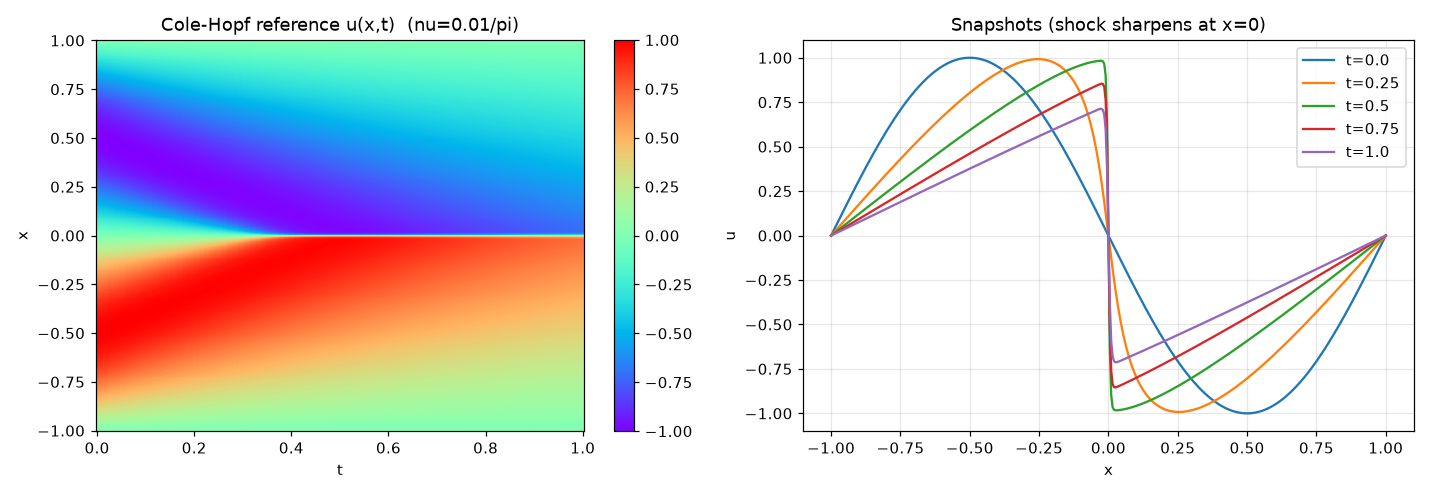
\includegraphics[width=\textwidth]{reference/burgers_reference.png}
\caption{\textbf{Exact Cole--Hopf reference} for Burgers ($\nu=0.01/\pi$): field $u(x,t)$ and snapshots. The shock forms at $x=0$ around $t\approx0.4$. Validated to machine precision (IC error 0, BC $\sim$1e-16, quadrature $\sim$1e-15). This is the ground truth every relative-$L_2$ is measured against.}
\end{figure}


\clearpage
\section{The XAI suite (five dimensions + dynamic monitoring)}
\emph{Full reference: \texttt{report/xai\_methods.md}.} Every method runs identically on
the cPINN and the QAPINN, so the two are comparable.
\begin{enumerate}[nosep]
\item \textbf{Spectral} (\texttt{spectrum.py}): realized per-harmonic magnitude vs
reference; per-harmonic error; \textbf{F-principle} (iteration at which each harmonic's
error halves --- low-before-high). The mechanistic core: does the VQC change the order?
\item \textbf{Neurons} (\texttt{neurons.py}): each classical neuron's receptive field
over $(x,t)$; its dominant spatial frequency; \emph{effective rank} (entropy-based count
of distinct features). More diverse features would be mechanistic support for parameter
reduction.
\item \textbf{VQC internals} (\texttt{vqc\_internals.py}): per-qubit
$\langle Z\rangle(x,t)$; von Neumann \emph{entanglement entropy} across the domain
(validated: entanglement=none $\to$ entropy $\approx0$). The literature skips this.
\item \textbf{Loss landscape} (\texttt{landscape.py}): filter-normalized 2-D slice
around the minimum (Li et al.\ 2018); flat/wide vs sharp.
\item \textbf{Generalization} (\texttt{generalization.py}): relative $L_2$ vs $t$ beyond
the training window --- does the Fourier prior extrapolate (quasi-)periodically?
\end{enumerate}
Dynamic monitoring records the spectrum build-up and per-tensor gradient variance
during training (barren-plateau / black-hole signal).

\clearpage
\section{Pipeline verification (the 8/8 audit)}
Before drawing any conclusion, every load-bearing computation was checked against an
external ground truth.
\begin{center}\small\begin{tabular}{lll}\toprule
Check & Method & Result \\ \midrule
Burgers residual & vs analytic & 1.2e-7 \\
Heat residual & exact $\to$ residual & 6.0e-8 \\
Autograd $u_x$ & vs finite differences & match \\
\textbf{VQC $=$ Fourier, max freq $=$ depth} & $L{=}2{\to}2$, $L{=}4{\to}4$ & \textbf{pass} \\
relative-$L_2$ metric & exact $\to 0$ & 4.0e-8 \\
Matched params & all configs & exact \\
Reproducibility & same seed, two machines & bit-exact \\
Constraint sampler & IC/BC coverage & pass \\
\bottomrule\end{tabular}\end{center}
\textbf{8/8 pass.} The VQC-bandwidth check validates the central premise on our own
implementation; the audit also caught a bug --- in the FFT-sampling \emph{test}, not the
code.

\clearpage
\section{Reading the fields --- observations and inferences}
Before the summary montages, this section works directly from individual run figures.
Each carries an \textbf{Observation} (what is visibly in the figure) and an
\textbf{Inference} (what we conclude from it). This is where the bandwidth thesis stops
being a table and becomes something you can \emph{see}.

\subsection{The clean contrast: same model, same IC, two spectra}
Heat and Burgers share the identical initial condition $u(x,0)=\sin(\pi x)$, the same
domain, the same boundary conditions, and here the \emph{identical} 121-parameter QAPINN
(depth 3, 4 qubits). The only difference is the operator --- and therefore the spectral
content the solution demands.
\begin{figure}[H]\centering
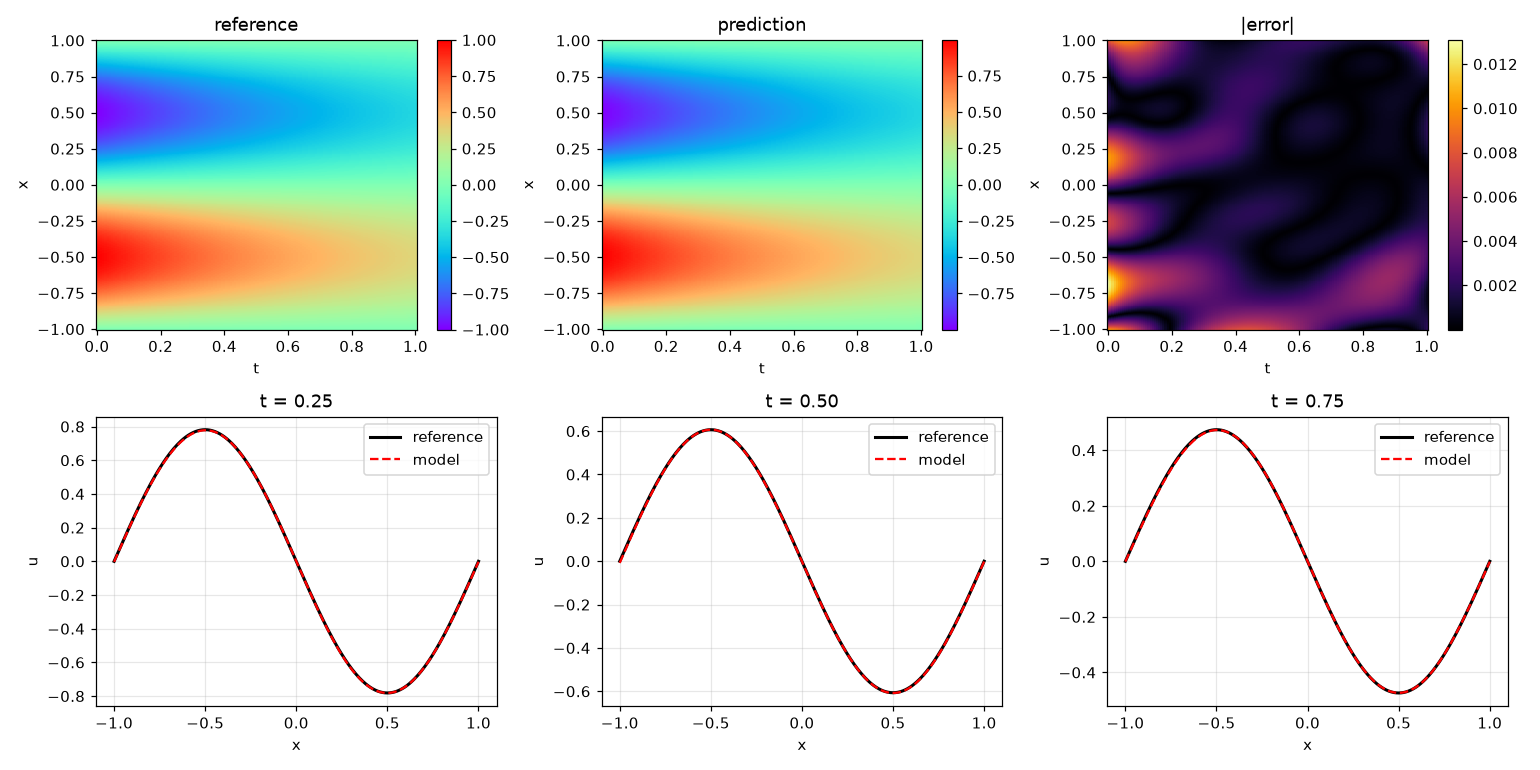
\includegraphics[width=\textwidth]{heat_qapinn/figures/solution.png}
\caption{\textbf{Heat, QAPINN.} Reference and prediction are visually indistinguishable; the error map (right) never exceeds $\sim$0.012 and carries no coherent structure --- just diffuse numerical residue. The $t=0.25/0.50/0.75$ snapshots show the red model curve lying exactly on the black reference.}
\end{figure}

\textbf{Observation.} The heat solution is a single decaying Fourier mode ($k=1$,
amplitude $e^{-t}$). The depth-3 QAPINN reproduces it essentially perfectly
(rel-$L_2 = 5.9\text{e-}3$): the snapshot curves overlap, and the residual is a
featureless ripple two orders of magnitude below the signal.
\begin{figure}[H]\centering
\includegraphics[width=\textwidth]{abl_baseline/figures/solution.png}
\caption{\textbf{Burgers, the same QAPINN.} Now the prediction colour-scale saturates at $\pm0.6$ while the reference spans $\pm1.0$: the model builds a smooth, \emph{amplitude-attenuated} version of the true field. The error (right) is a single bright band pinned to the shock at $x=0$; everywhere else it is dark. In the snapshots the red model tracks the linear ramps away from the shock almost exactly, then rounds the jump and undershoots the extrema ($\sim$0.6 vs 1.0).}
\end{figure}

\textbf{Observation.} Same network, same initialisation, same training budget --- but on
Burgers the identical model lands at rel-$L_2 = 0.47$, an 80$\times$ worse error than on
heat. The failure is spatially localised: away from $x=0$ (the low-frequency region) the
fit is excellent; \emph{all} of the error lives in the shock.

\textbf{Inference.} Accuracy here is not a property of the model --- it is a property of
the \emph{match between the solution's bandwidth and the circuit's band}. The heat
solution lives entirely inside the depth-3 band $\{-3..3\}$, so the model is near-exact;
the Burgers shock needs harmonics far beyond it, so the same model saturates. This single
pair is the strongest visual statement of the thesis: the quantum layer's usefulness is
gated by bandwidth, and bandwidth is set by the physics of the target, not the optimiser.

\subsection{Why, in frequency space}
The solution fields hint at a spectral cutoff; the realized-spectrum plot makes it
explicit.
\begin{figure}[H]\centering
\includegraphics[width=\textwidth]{abl_baseline/figures/spectrum.png}
\caption{\textbf{Realized Fourier spectrum, baseline QAPINN (depth 3).} Grey $=$ exact reference, red $=$ trained model, log-scale magnitude per spatial harmonic $k$. The reference decays only as $\sim1/k$ --- the slow tail of a near-discontinuity, with real power out to $k=20$. The model \emph{matches} the reference at $k=1,2,3$ then falls progressively below it, flattening to a floor $\sim$0.1--0.3 for $k\gtrsim7$.}
\end{figure}

\textbf{Observation.} The crossover from ``model matches'' to ``model undershoots'' sits
right around $k=3\text{--}4$ --- exactly the edge of the depth-3 accessible band. Beyond it
the model retains only a small residual (leaked through the classical post-net's
nonlinearity), one to two orders of magnitude short of the reference.

\textbf{Inference.} This is the mechanism behind the rounded shock, read directly off the
coefficients. A truncated Fourier series cannot represent a jump; it approximates it with
its available harmonics, which both smears the discontinuity and --- because the missing
high-$k$ power also carries amplitude --- pulls down the peak values. The rounded shock and
the amplitude undershoot are not two bugs; they are the \emph{same} band-truncation seen
in space and in frequency. It also confirms Mhiri's caveat operationally: the model
\emph{does} put nonzero coefficients at high $k$, but their \emph{magnitude} is far too
small --- frequency support is not the same as realized coefficient power.

\subsection{Add band, sharpen the shock}
If band-truncation is the mechanism, extending the band (more re-upload depth) should
tighten the shock. It does --- modestly.
\begin{figure}[H]\centering
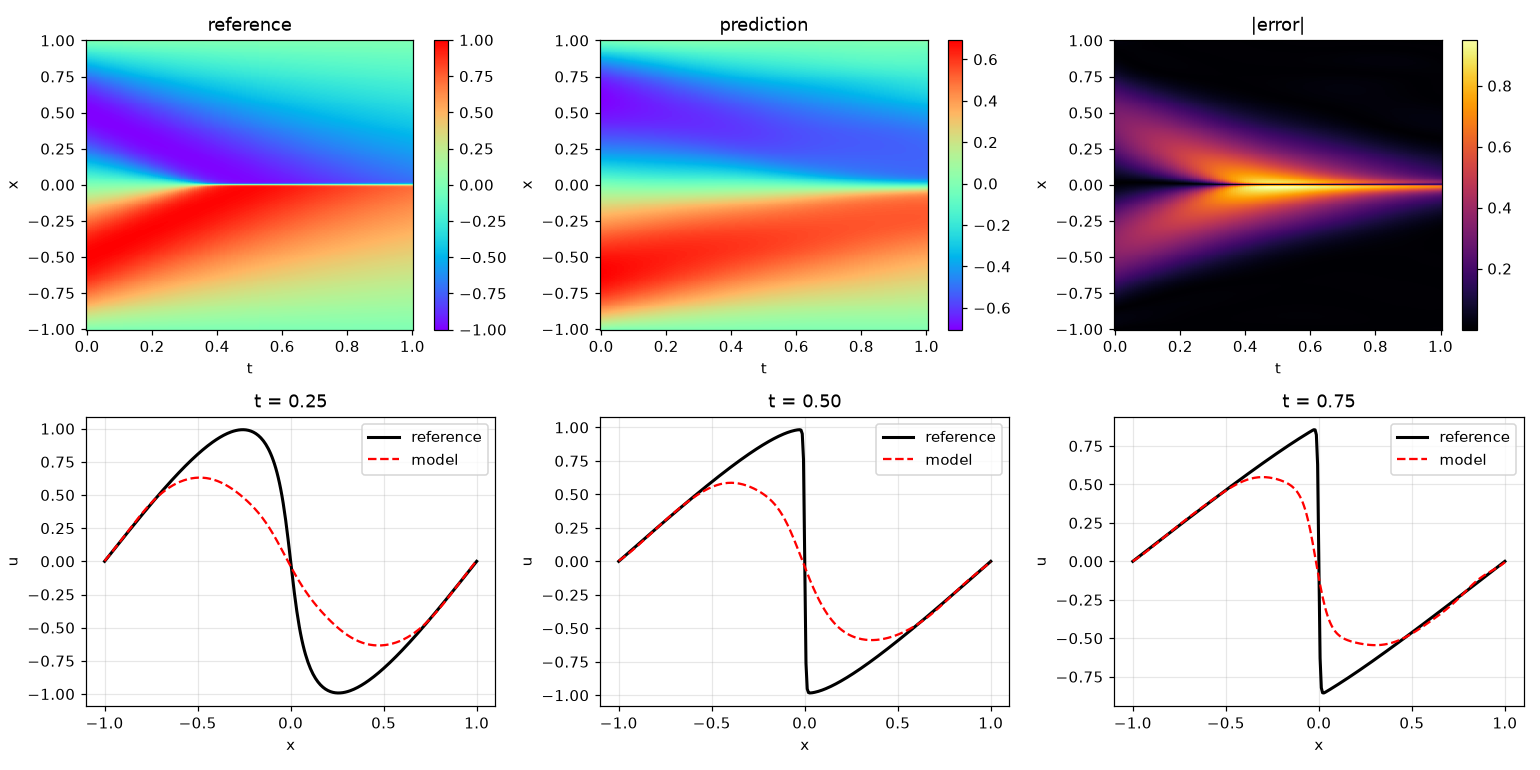
\includegraphics[width=\textwidth]{abl_depth_5/figures/solution.png}
\caption{\textbf{Burgers, depth-5 QAPINN.} Against the depth-3 baseline above, the bright error band at the shock is visibly \emph{narrower} and the snapshot transition through $x=0$ is steeper. The peak amplitude is still capped near $\pm0.6$, but the jump is resolved over a shorter interval.}
\end{figure}

\textbf{Observation.} Two extra re-uploads move rel-$L_2$ from 0.472 to 0.424 --- a real
but undramatic gain --- and the improvement is exactly where theory says it should be:
concentrated at the shock, sharpening the transition rather than lifting the whole field.

\textbf{Inference.} The advantage of depth is spectral and \emph{local}: it buys the
harmonics that live at the discontinuity, nothing else. This is why the depth sweep is
monotonic and physically legible while entanglement (below) is not --- depth changes what
the model \emph{can} represent, at the precise place it was failing.

\subsection{Push the encoding too hard: the black-hole collapse}
Bandwidth knobs help --- until trainability gives out. The encoding-scale sweep exposes the
ceiling in the most dramatic figure in the project.
\begin{figure}[H]\centering
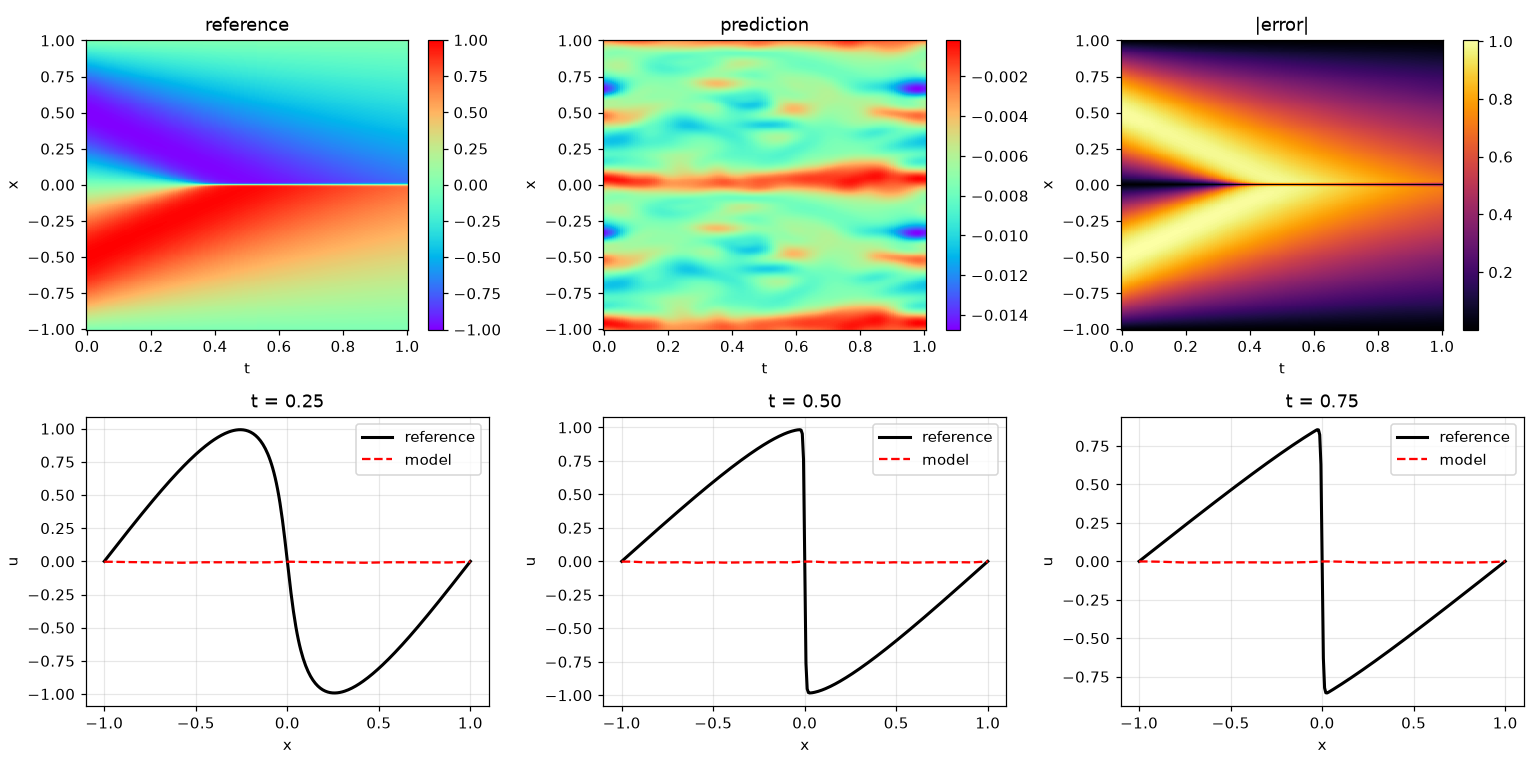
\includegraphics[width=\textwidth]{abl_scale_2pi/figures/solution.png}
\caption{\textbf{Burgers, input\_scale $=2\pi$.} The prediction colour-scale now reads $-0.014$ to $-0.002$: the entire field has collapsed to $u\approx0$, with only faint high-frequency speckle. In every snapshot the red model is a flat line at zero while the reference sweeps $\pm1$. The error is $\approx$1 everywhere except the $x=0$ line (where the true solution is itself zero).}
\end{figure}

\textbf{Observation.} At scale 1 the model reaches rel-$L_2$ 0.47; at scale $2\pi$ it is
1.00 --- a total collapse to the trivial solution. The transition is not gradual
degradation but a fall into a different basin: the network satisfies the homogeneous
boundary conditions and abandons the initial condition entirely.

\textbf{Inference.} This is the literature's ``black-hole'' collapse (Chen et al.\ 2026)
reproduced on demand. At $2\pi$ the encoding wraps the input across a full period, so
neighbouring collocation points map to widely separated circuit states; the loss surface
around the true solution flattens and the optimiser slides into the zero basin. The
practical lesson for the design methodology is sharp: \textbf{encoding scale is not a free
hyperparameter} --- there is an optimum near 1 and a hard cliff past it, and a
circuit-sizing recipe must respect that cliff or it will silently recommend an untrainable
model.

\subsection{The circuit works hard internally --- and it barely matters}
The quantum-internal views let us watch the circuit's own state, not just its output. They
deliver the study's most counter-intuitive observation.
\begin{figure}[H]\centering
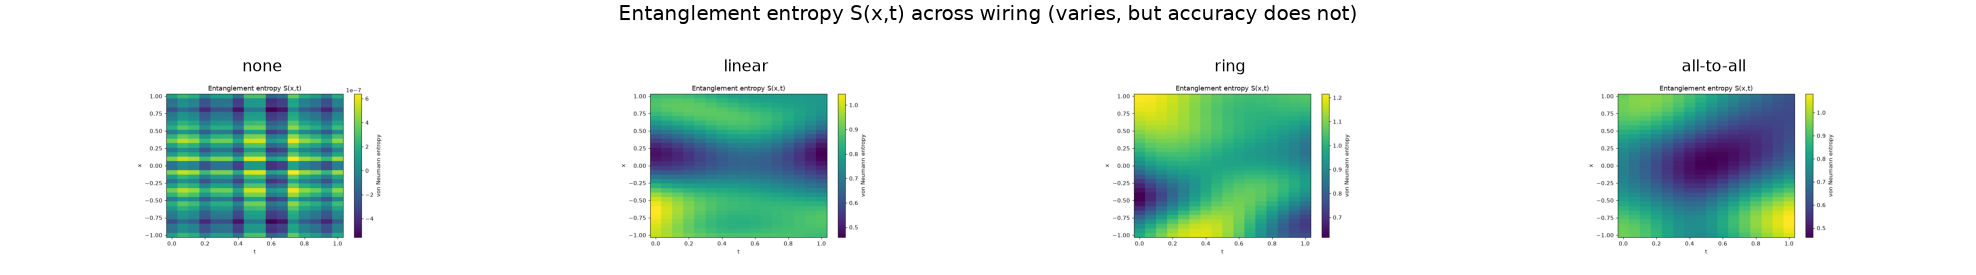
\includegraphics[width=\textwidth]{ablation_summary/ent_entropy_fields.png}
\caption{\textbf{Von Neumann entanglement entropy $S(x,t)$ across wiring.} \emph{none}: the scale is $10^{-7}$ --- numerically zero, exactly as an unentangled circuit must be (a clean sanity check). \emph{linear/ring/all-to-all}: entropy climbs to $\sim$1.0--1.2 nats with rich spatial structure --- the ring case shows a diagonal high-entropy ridge that follows the shock's space--time trajectory.}
\end{figure}

\textbf{Observation.} Internally these four circuits are doing wildly different things: the
entangled variants generate up-to-$>$1-nat, spatially-structured entanglement whose pattern
tracks the physics, while the unentangled one sits at machine-zero. Yet across seven seeds
their accuracies are statistically indistinguishable (none $0.459\pm0.011$, linear
$0.448\pm0.022$, ring $0.474\pm0.014$, all-to-all $0.462\pm0.014$).

\textbf{Inference.} Internal quantum complexity is, in this regime, \emph{decoupled} from
task performance. The binding constraint is the band --- already saturated at depth 3 ---
so redistributing which coefficients are reachable (what entanglement does) moves the
answer within noise. This is a genuinely deflationary result for the field's favourite
heuristic (``entanglement-driven expressibility''): here you can dial entanglement from
zero to strongly-structured and the PINN does not care. The honest reading is not
``entanglement is useless'' but ``once the band is the bottleneck, the coefficient
machinery is not what is limiting you'' --- and diagnosing \emph{which} regime you are in is
the useful contribution.

\subsection{It is bandwidth, not capacity --- the classical controls prove it}
A natural objection to the whole bandwidth story: maybe the shock is just hard, and any
model --- quantum or classical --- would fix it with \emph{more parameters}. Reading all
eleven matched classical controls (29 to 217 parameters) refutes that directly. Shock
quality is \emph{non-monotonic} in parameter count.
\begin{figure}[H]\centering
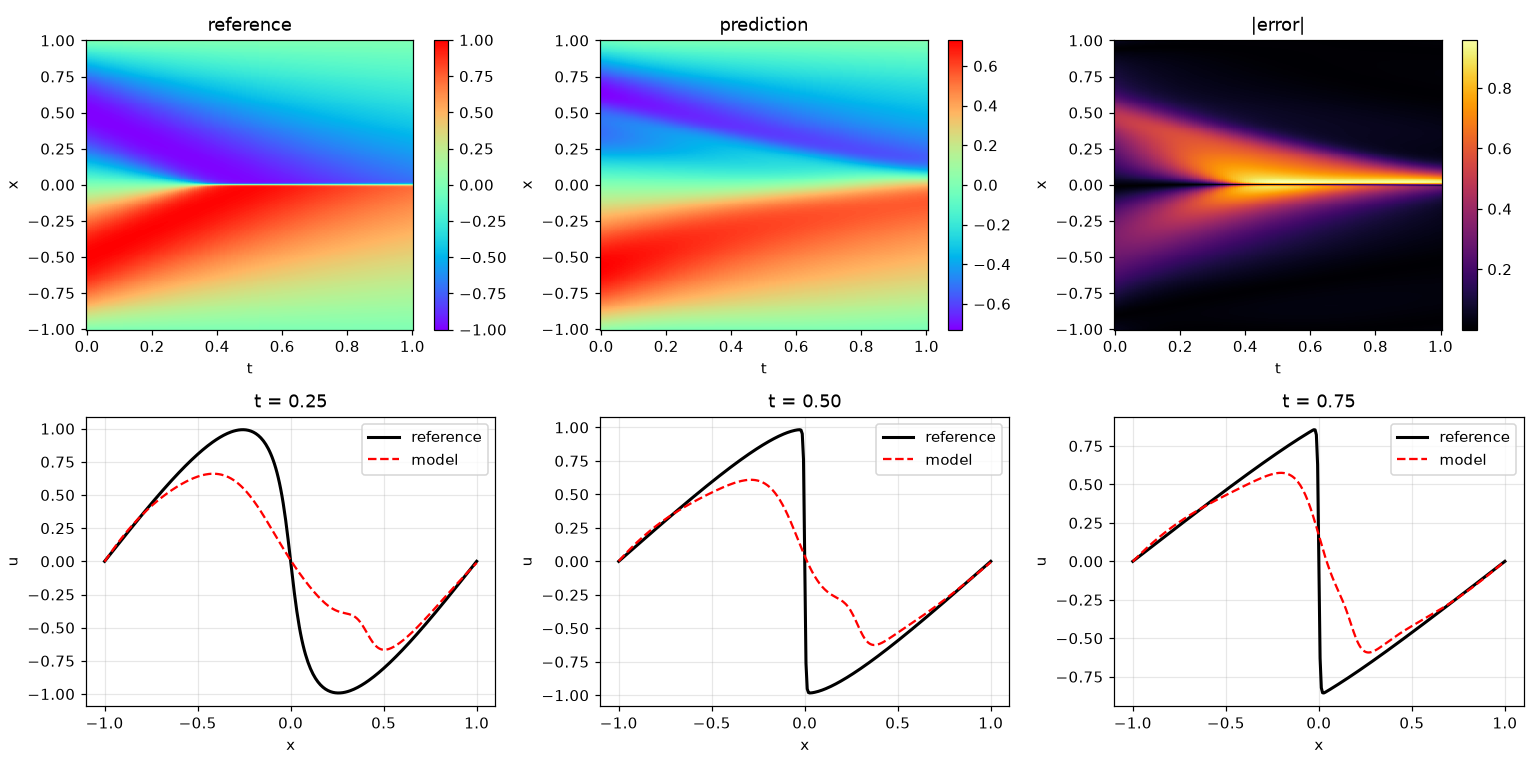
\includegraphics[width=\textwidth]{abl_cls_165/figures/solution.png}
\caption{\textbf{Classical, 165 params --- the best shock of the sweep.} The front is visibly tilted and steepened with a slight overshoot near $x\approx0.3$--0.5, the closest any matched classical net comes to the reference discontinuity; peak $\sim$0.68 and the error band is the tightest of the eleven.}
\end{figure}
\begin{figure}[H]\centering
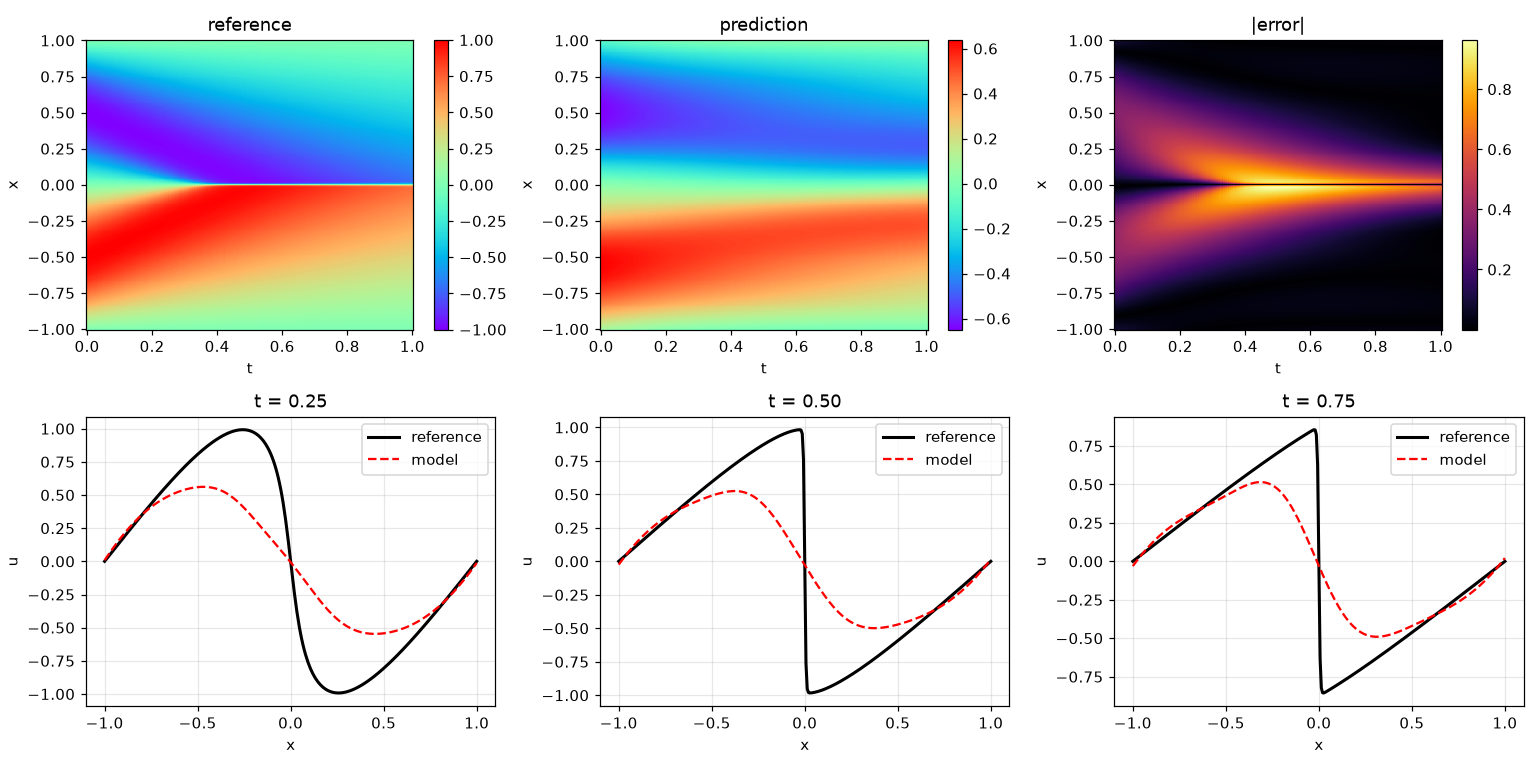
\includegraphics[width=\textwidth]{abl_cls_217/figures/solution.png}
\caption{\textbf{Classical, 217 params --- the largest net, and mediocre.} Nearly twice the capacity of the 165-param net, yet the shock is rounded into a smooth curve with no steepening (peak $\sim$0.57) and a broader error plume. More parameters did not buy a sharper shock.}
\end{figure}

\textbf{Observation.} Across the eleven controls the sharpest shocks come from
\emph{mid-sized} nets (165 params $\sim$0.68, 99 params $\sim$0.73), while the
\emph{largest} (217) is unremarkable ($\sim$0.57) and one larger net (143) collapses to a
near-static underfit ($\sim$0.46). All eleven round the shock and cap amplitude; none
approach the reference's $\pm1.0$ jump; and every one matches only $k=1$ before falling a
half-to-full decade below the reference for $k\gtrsim4$.

\textbf{Inference.} Capacity is \emph{not} the limiting factor for shock resolution ---
this is spectral bias (the F-principle), not an under-parameterisation. That reframes what
the quantum layer is even competing on: the question was never ``can more parameters fix
the shock'' (they cannot, reliably) but ``can a different \emph{basis} reach the missing
high harmonics''. It is why the honest comparison is bandwidth-for-bandwidth (depth,
qubits) against a \emph{structurally} matched control, not parameter-for-parameter against
an arbitrary MLP --- and why the depth axis, which literally extends the band, is the only
knob that improves the shock monotonically.

\clearpage
\section{Results --- comparative figures (montages)}
The following montages place classical and QAPINN side by side across the whole XAI
suite. Per-run originals for every model are in the gallery (Part~II).
\begin{figure}[H]\centering
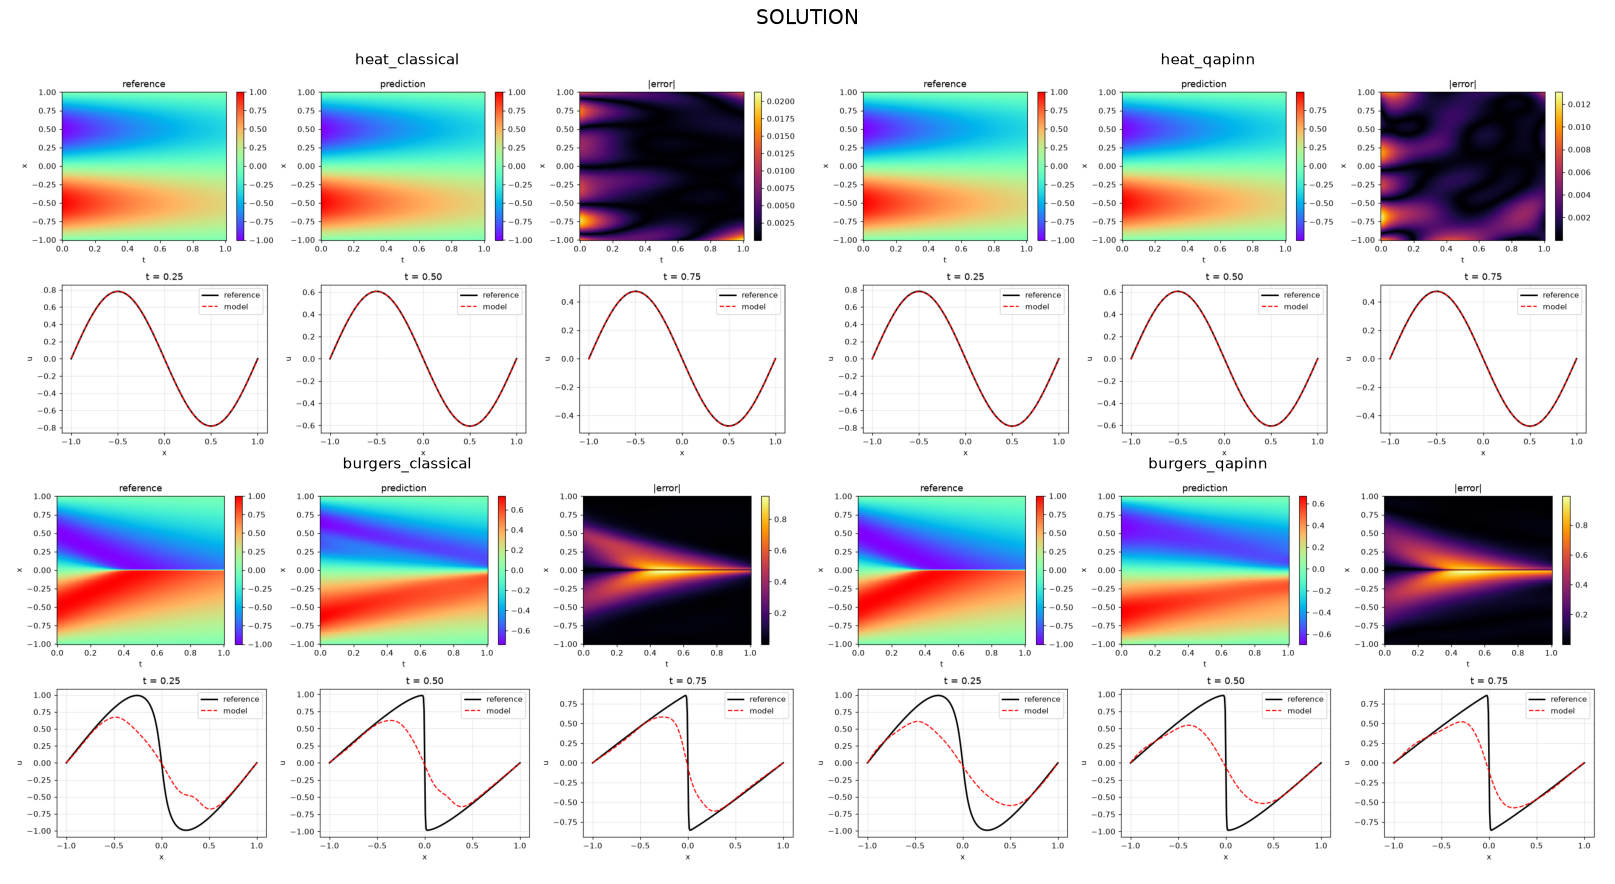
\includegraphics[width=\textwidth]{_montage/solution.png}
\caption{\textbf{Solution fields.} Heat (top): both fit near-perfectly. Burgers (bottom): both round the shock --- the depth-3 band is capped near $k\approx3$.}
\end{figure}

\begin{figure}[H]\centering
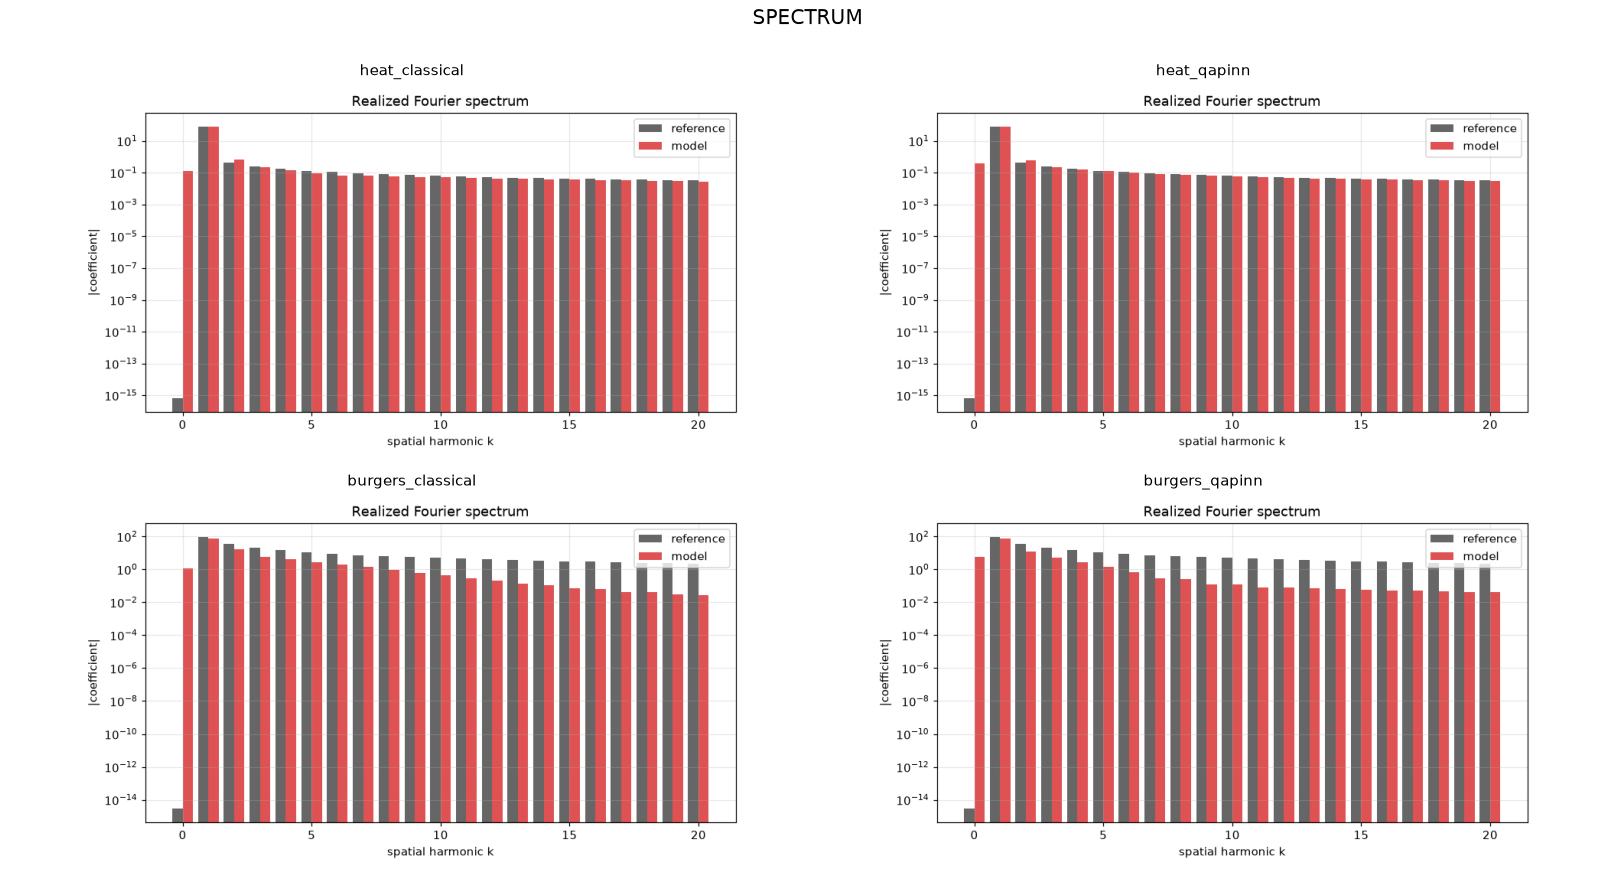
\includegraphics[width=\textwidth]{_montage/spectrum.png}
\caption{\textbf{Realized spectra.} Heat: single mode both capture. Burgers: reference is broadband; both models undershoot the high-frequency shock tail.}
\end{figure}

\begin{figure}[H]\centering
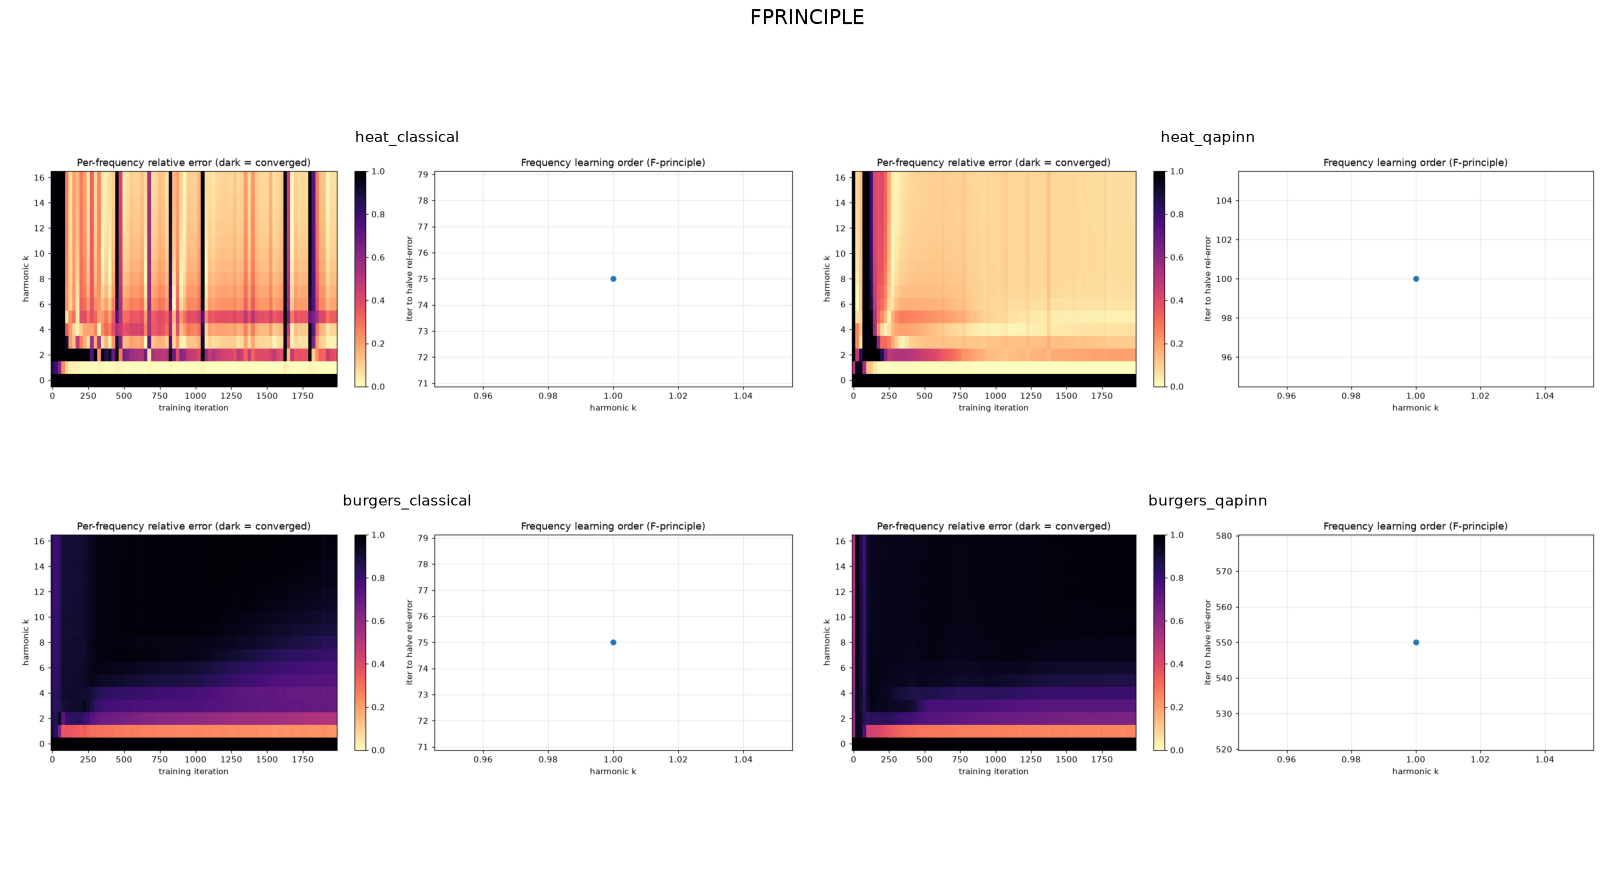
\includegraphics[width=\textwidth]{_montage/fprinciple.png}
\caption{\textbf{F-principle.} The error-reduction wave sweeps from low $k$ upward --- low frequencies converge first, in both models.}
\end{figure}

\begin{figure}[H]\centering
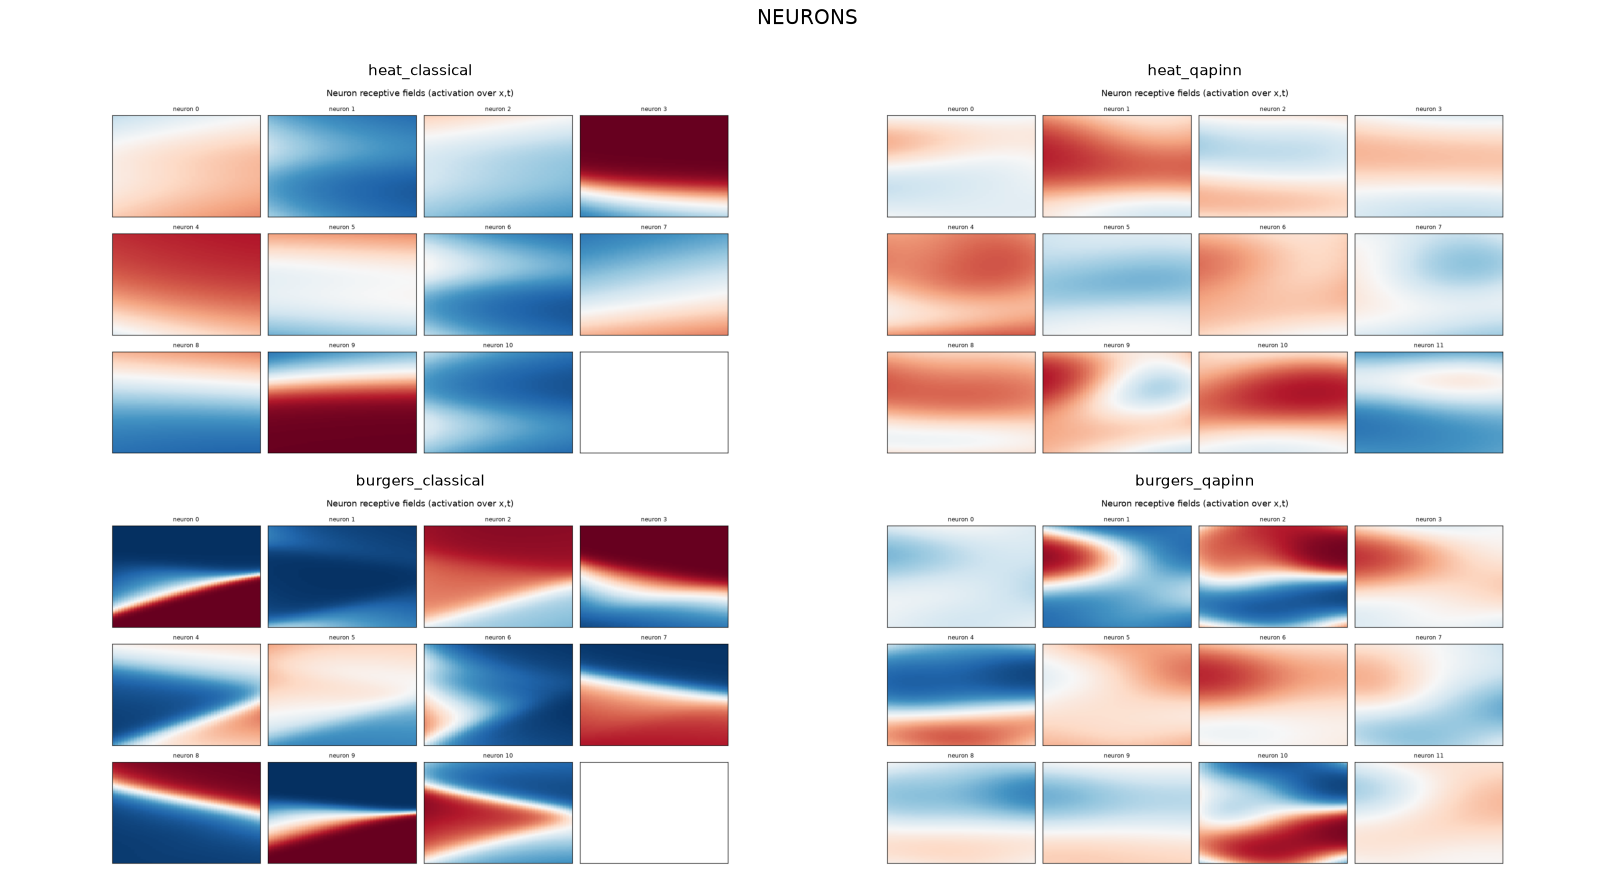
\includegraphics[width=\textwidth]{_montage/neurons.png}
\caption{\textbf{Classical neurons.} Receptive fields and dominant-frequency histograms, classical vs QAPINN post-net.}
\end{figure}

\begin{figure}[H]\centering
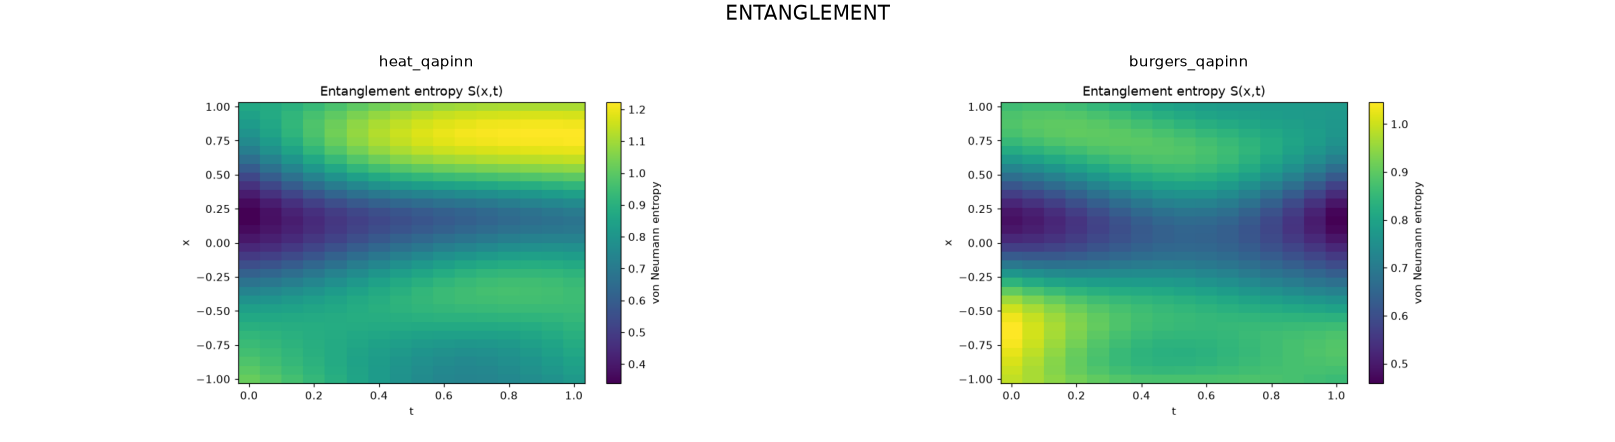
\includegraphics[width=\textwidth]{_montage/entanglement.png}
\caption{\textbf{Entanglement entropy $S(x,t)$} (QAPINN): the state entangles differently per problem.}
\end{figure}

\begin{figure}[H]\centering
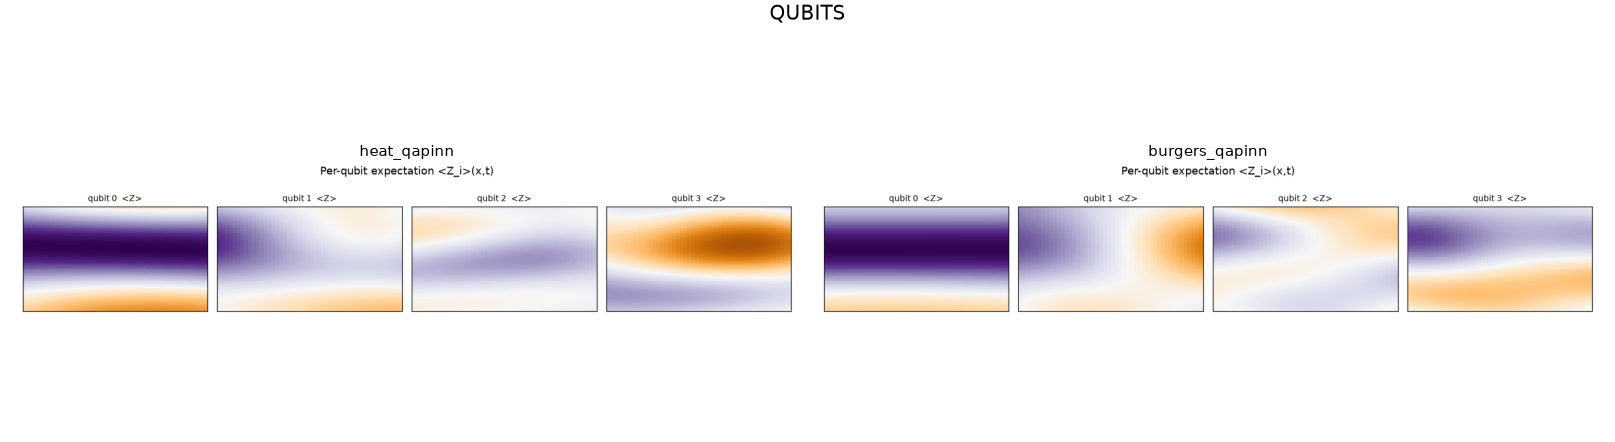
\includegraphics[width=\textwidth]{_montage/qubits.png}
\caption{\textbf{Per-qubit $\langle Z\rangle$ fields}: what feature each qubit specializes in.}
\end{figure}

\begin{figure}[H]\centering
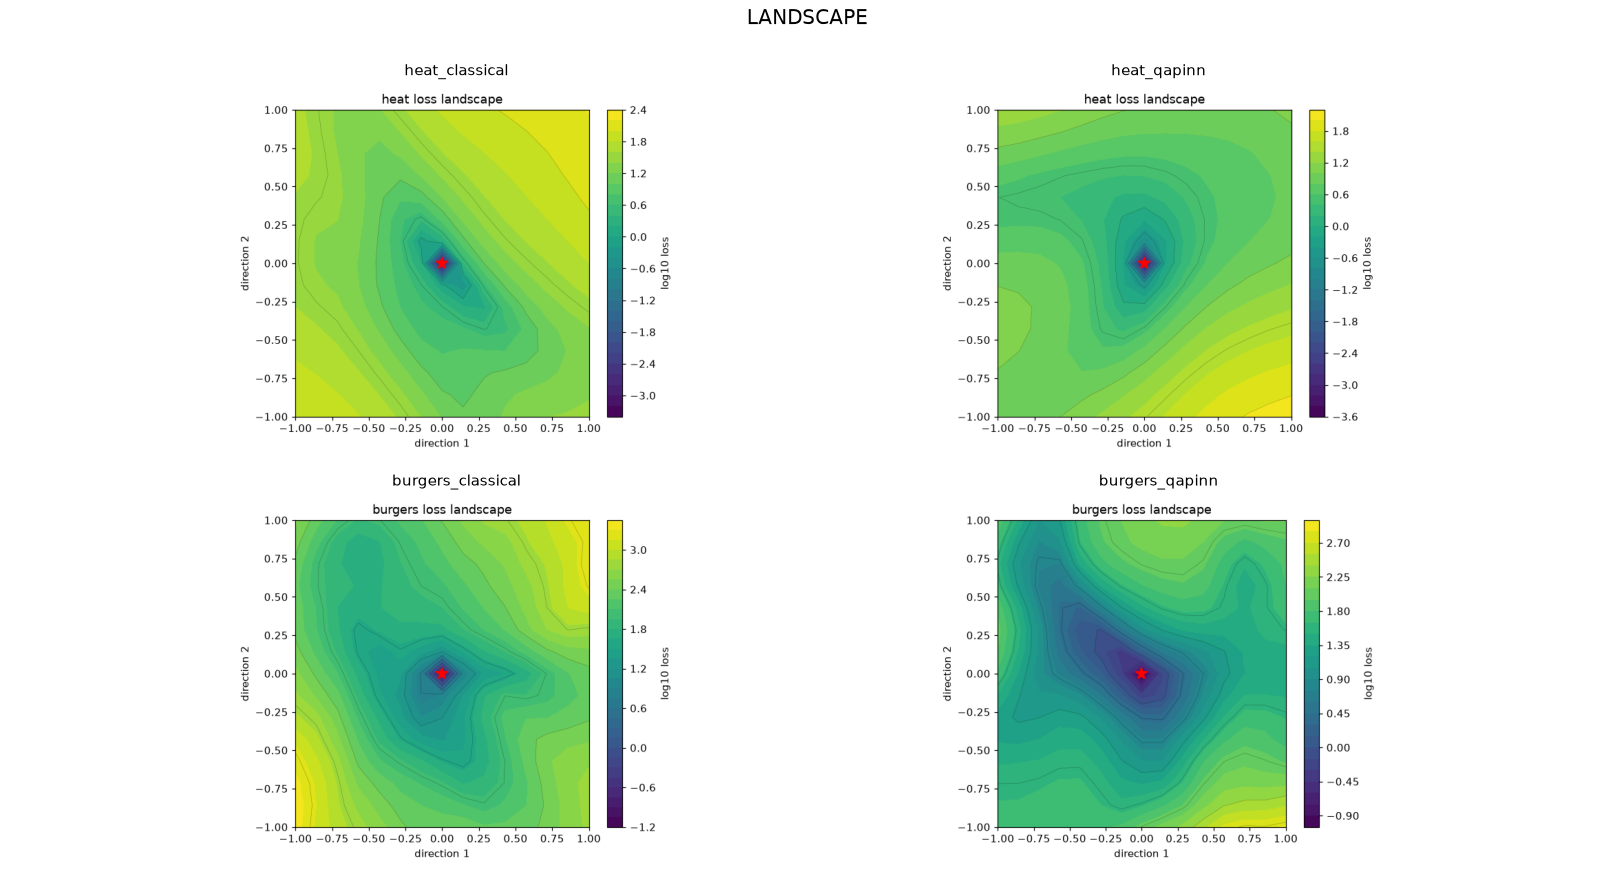
\includegraphics[width=\textwidth]{_montage/landscape.png}
\caption{\textbf{Loss landscapes} around the minimum, classical vs QAPINN.}
\end{figure}

\begin{figure}[H]\centering
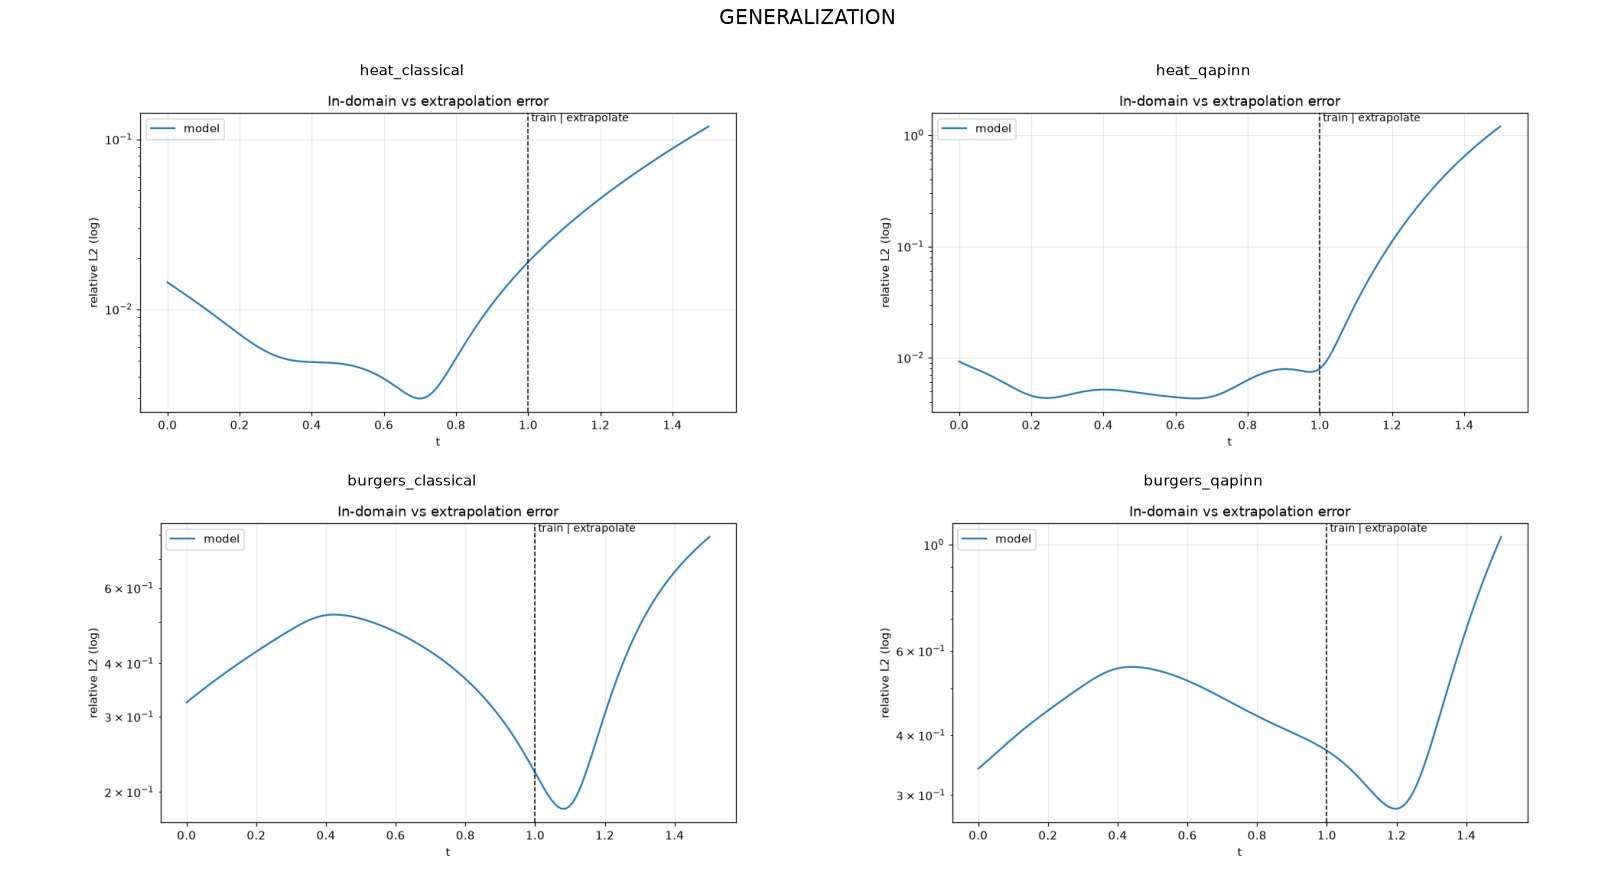
\includegraphics[width=\textwidth]{_montage/generalization.png}
\caption{\textbf{Generalization}: relative $L_2$ vs $t$ past the training window.}
\end{figure}

\begin{figure}[H]\centering
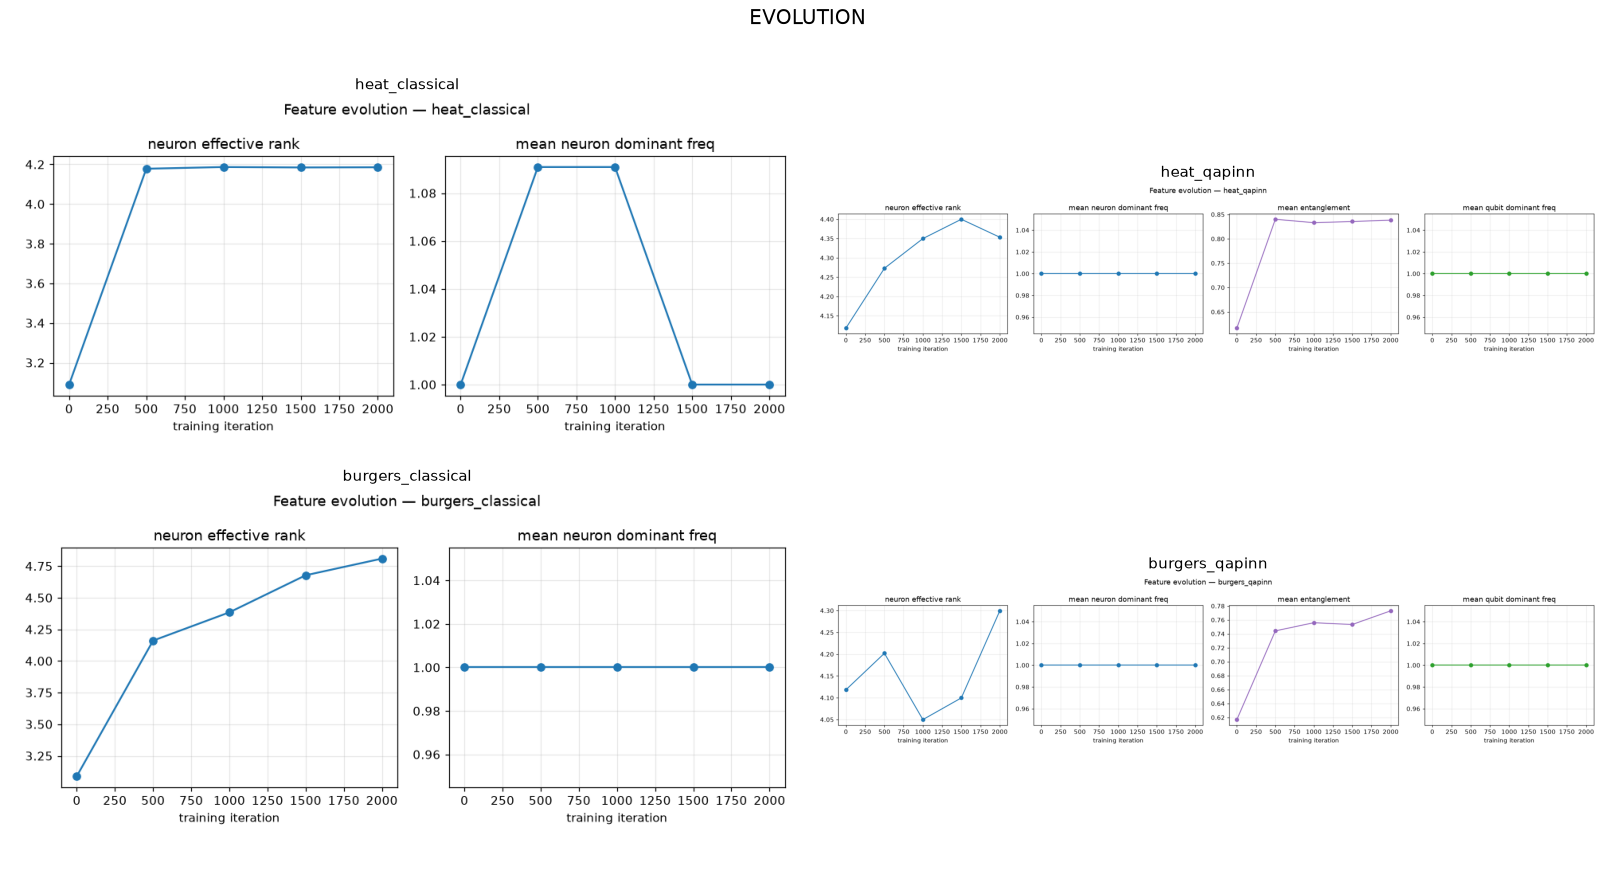
\includegraphics[width=\textwidth]{_montage/evolution.png}
\caption{\textbf{Solution evolution} snapshots over time.}
\end{figure}

\begin{figure}[H]\centering
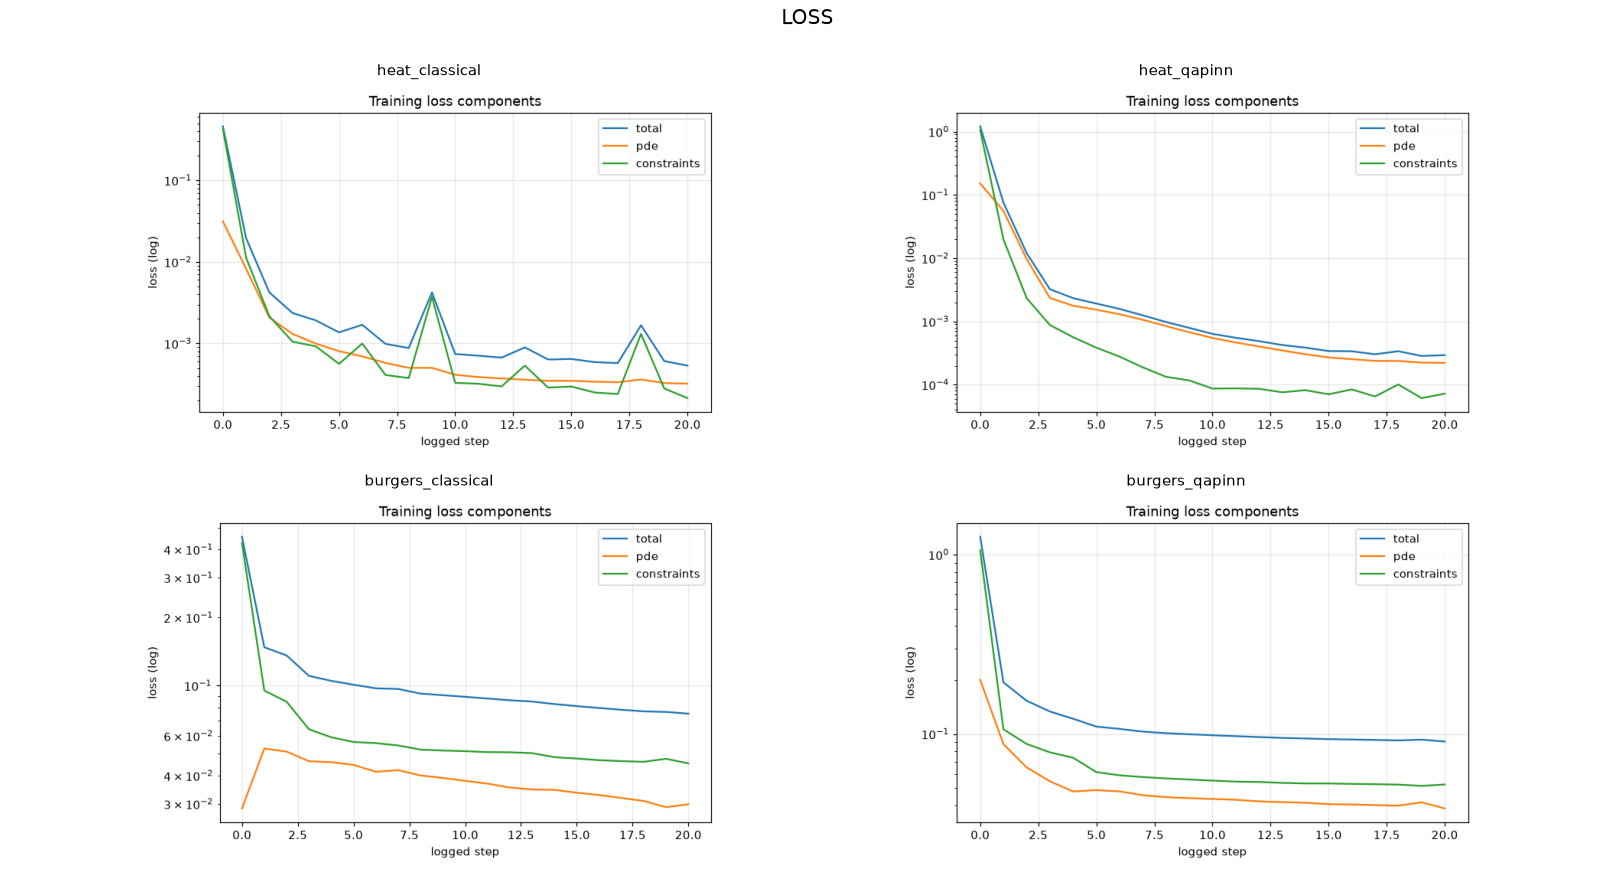
\includegraphics[width=\textwidth]{_montage/loss.png}
\caption{\textbf{Training-loss histories}, classical vs QAPINN.}
\end{figure}


\clearpage
\section{Ablation results --- summary panels}
One knob at a time; each QAPINN paired with a param-matched classical control.
\begin{figure}[H]\centering
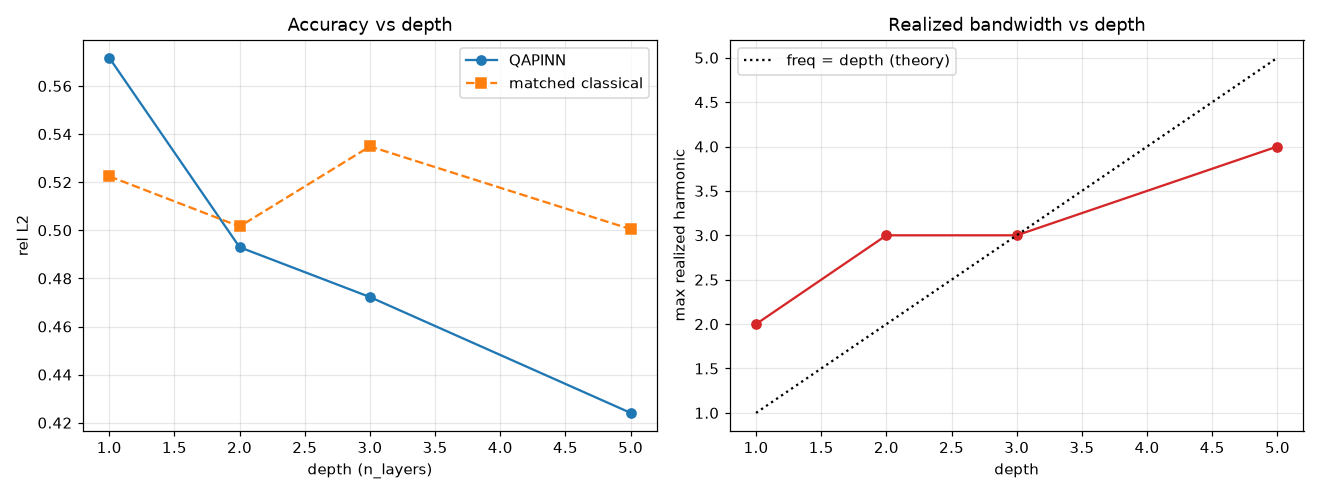
\includegraphics[width=\textwidth]{ablation_summary/depth_sweep.png}
\caption{\textbf{Depth sweep.} QAPINN accuracy and realized bandwidth grow with re-upload depth; overtakes the matched classical at depth $\geq3$. \emph{Robust, physically grounded.}}
\end{figure}

\begin{figure}[H]\centering
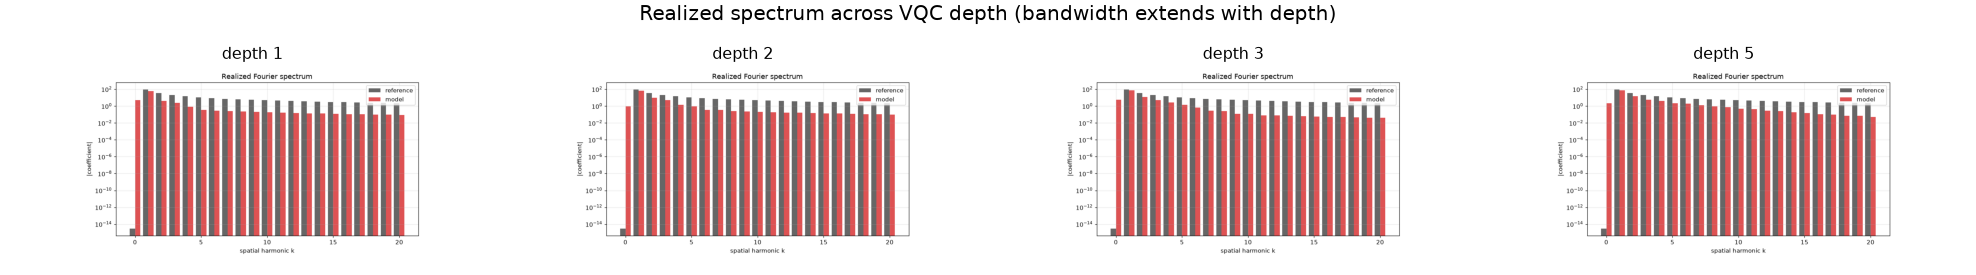
\includegraphics[width=\textwidth]{ablation_summary/depth_spectra.png}
\caption{\textbf{Realized spectrum across depth} --- more of the high-frequency shock tail is captured as depth grows.}
\end{figure}

\begin{figure}[H]\centering
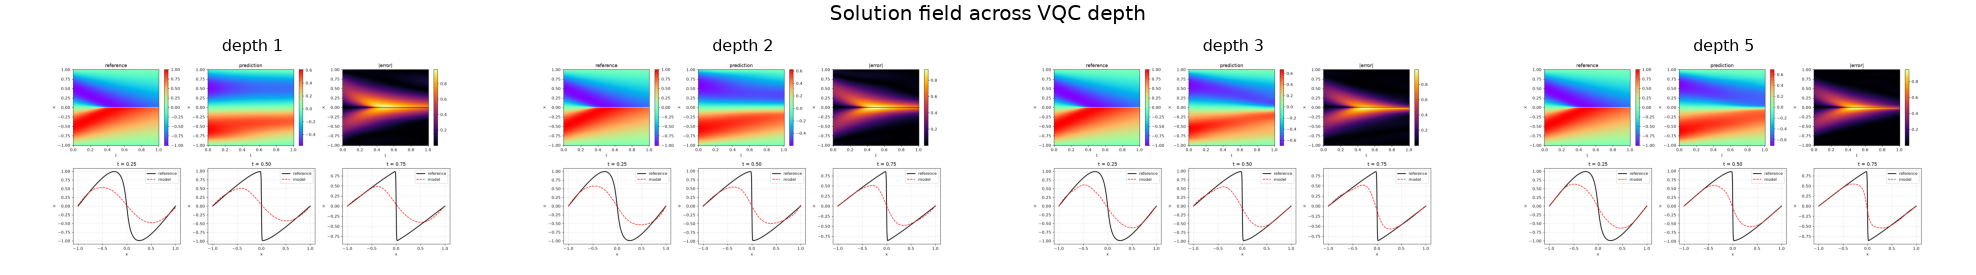
\includegraphics[width=\textwidth]{ablation_summary/depth_solutions.png}
\caption{\textbf{Solution field across depth.}}
\end{figure}

\begin{figure}[H]\centering
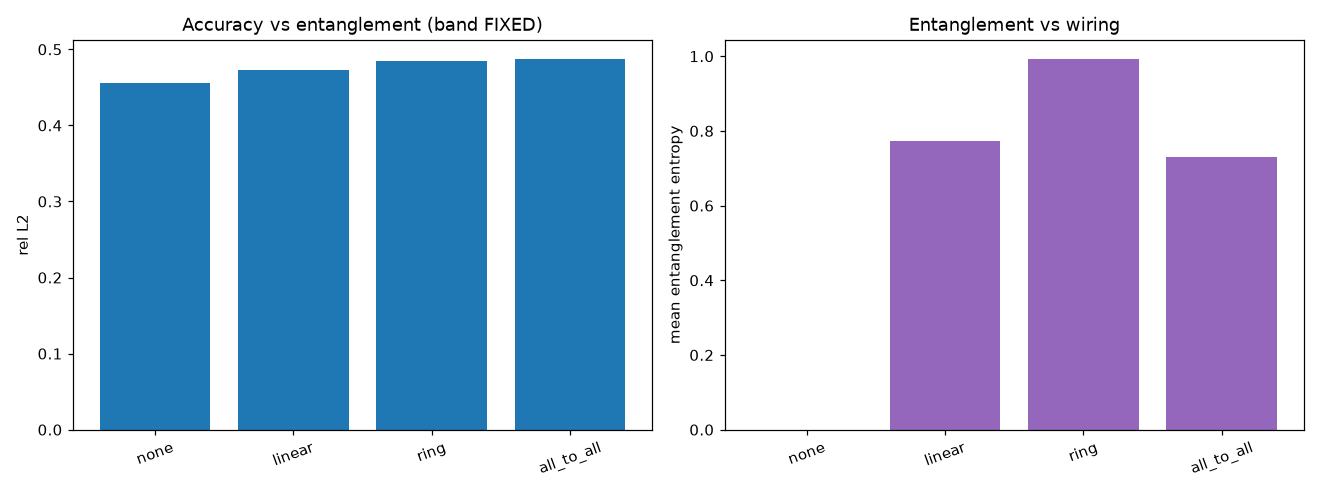
\includegraphics[width=\textwidth]{ablation_summary/entanglement_sweep.png}
\caption{\textbf{Entanglement (band fixed).} Accuracy barely moves while entropy swings widely --- \emph{single-seed}; later found within noise (see seeds).}
\end{figure}

\begin{figure}[H]\centering
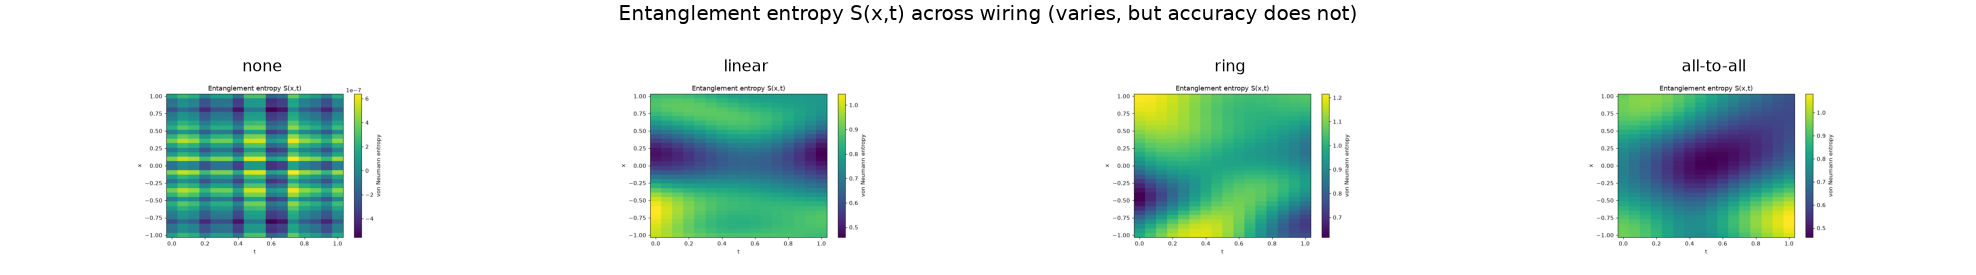
\includegraphics[width=\textwidth]{ablation_summary/ent_entropy_fields.png}
\caption{\textbf{Entanglement-entropy fields} across wiring: entropy varies strongly even as accuracy does not.}
\end{figure}

\begin{figure}[H]\centering
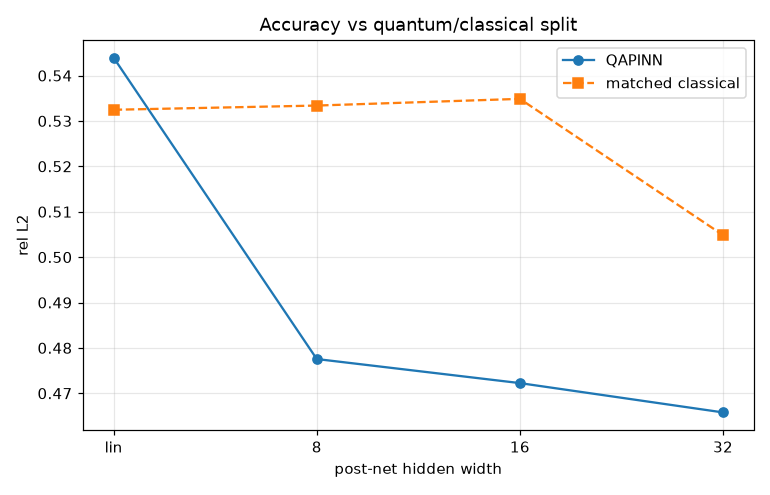
\includegraphics[width=\textwidth]{ablation_summary/post_sweep.png}
\caption{\textbf{Post-net width.} The VQC needs a small readout but beats the matched classical for any post-net $\geq[8]$.}
\end{figure}

\begin{figure}[H]\centering
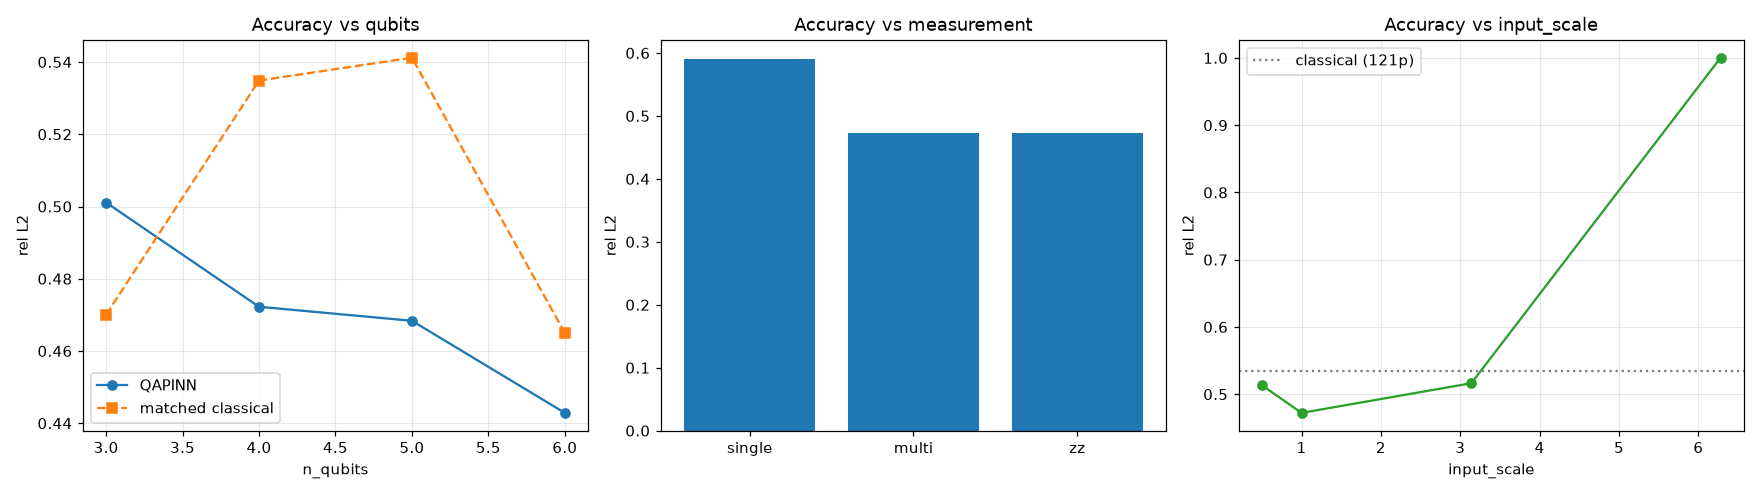
\includegraphics[width=\textwidth]{ablation_summary/tier3_sweeps.png}
\caption{\textbf{Tier-3 sweeps.} Qubits behave like depth (bandwidth). Single-$Z$ readout bottlenecks; multi $=$ $ZZ$. Encoding scale has an optimum near 1 and \emph{collapses} at $2\pi$ (black-hole).}
\end{figure}

\begin{figure}[H]\centering
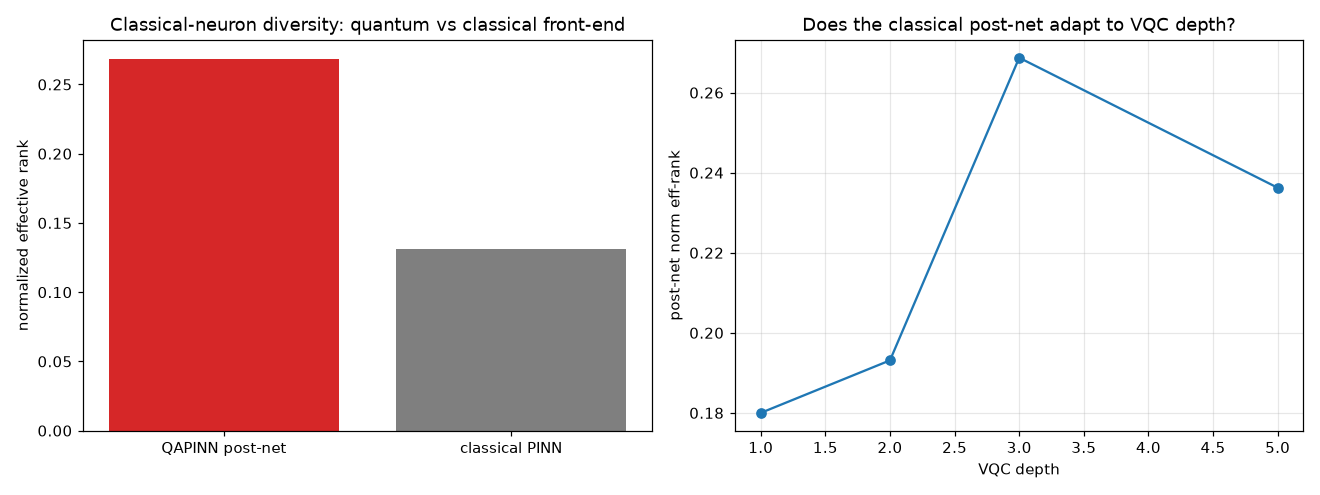
\includegraphics[width=\textwidth]{ablation_summary/classical_response.png}
\caption{\textbf{Classical-side response} (first pass, vs a plain PINN).}
\end{figure}

\begin{figure}[H]\centering
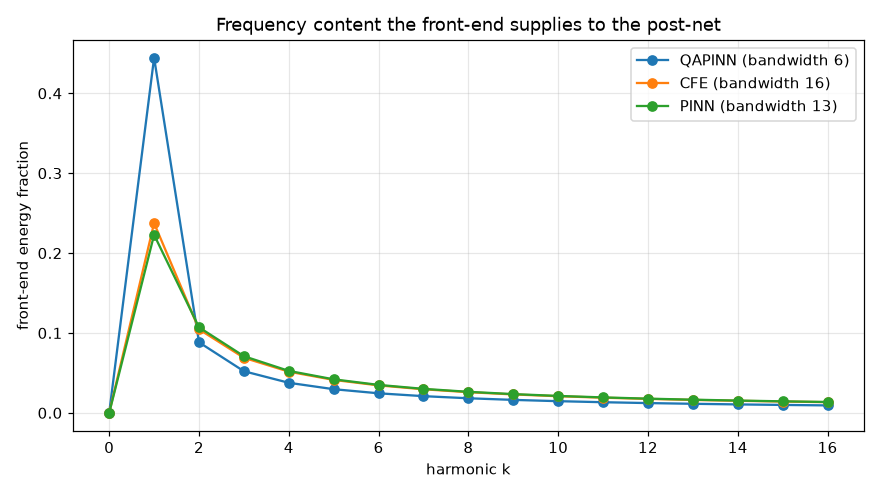
\includegraphics[width=\textwidth]{ablation_summary/frontend_spectra.png}
\caption{\textbf{Front-end spectra}: what the VQC vs a classical front-end feed into the identical post-net.}
\end{figure}

\begin{figure}[H]\centering
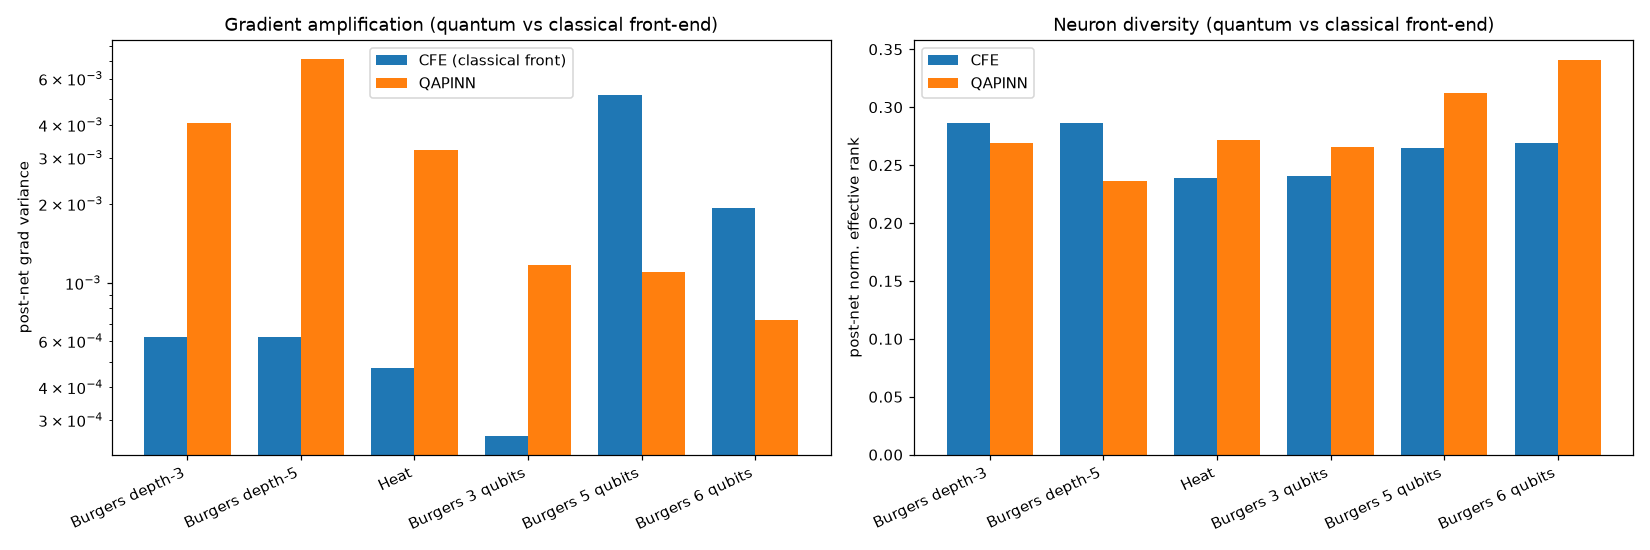
\includegraphics[width=\textwidth]{ablation_summary/cfe_comparison.png}
\caption{\textbf{The decisive fair control.} Quantum vs classical front-end on the \emph{identical} post-net. Gradient amplification and neuron diversity are \emph{neither} robust across knobs --- this refuted the classical-side-diversity claim.}
\end{figure}

\begin{figure}[H]\centering
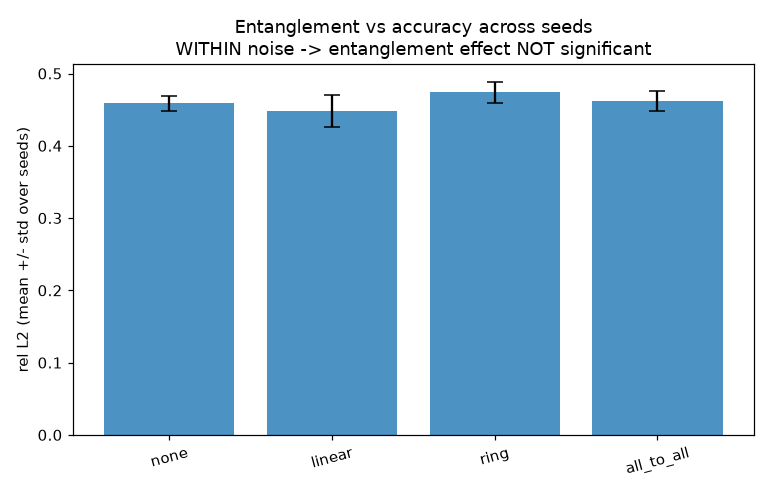
\includegraphics[width=\textwidth]{ablation_summary/entanglement_seeds.png}
\caption{\textbf{Entanglement across 7 seeds} with error bars: the differences are within seed noise --- \emph{entanglement effect NOT significant at 2000 iters}.}
\end{figure}


\clearpage
\section{Deflation --- the classical-side mechanism, and its fair control}
\textbf{Hypothesis.} The VQC ``offloads'' basis construction, so the downstream classical
neurons become more diverse and are driven with larger gradients.

Against a \emph{plain PINN} this looked true ($\sim$2$\times$ diversity, $\sim$4$\times$
gradient variance). But the plain PINN differs from the QAPINN in \emph{two} ways (front
end \emph{and} depth), so the attribution was confounded. We built the \textbf{CFE}: the
identical post-net fed by a classical $\mathrm{Linear}(2\!\to\!w)+\tanh$ --- same
structure, classical front end. Against \emph{that} fair control:
\begin{center}\small\begin{tabular}{lccc}\toprule
Comparison & rel-$L_2$ (Q/C) & diversity (Q/C) & grad-var $\times10^{-3}$ (Q/C) \\ \midrule
Burgers depth-3 & 0.472 / 0.474 & 0.269 / \textbf{0.286} & \textbf{4.1} / 0.62 \\
Burgers depth-5 & \textbf{0.424} / 0.474 & 0.236 / \textbf{0.286} & \textbf{7.1} / 0.62 \\
Heat & \textbf{0.006} / 0.013 & \textbf{0.272} / 0.239 & \textbf{3.2} / 0.47 \\
3 qubits & 0.501 / 0.496 & \textbf{0.266} / 0.241 & \textbf{1.2} / 0.26 \\
5 qubits & 0.468 / 0.464 & \textbf{0.312} / 0.265 & 1.1 / \textbf{5.2} \\
6 qubits & \textbf{0.443} / 0.467 & \textbf{0.341} / 0.269 & 0.72 / \textbf{1.9} \\
\bottomrule\end{tabular}\end{center}
\verdict{The mechanism deflated.} (i) Diversity is \emph{inconsistent} --- the classical
front end is \emph{more} diverse on the depth axis; the ``2$\times$'' was an artifact of
the mismatched plain-PINN control. (ii) Gradient amplification \emph{reverses} at 5--6
qubits, where the QAPINN's gradient variance \emph{shrinks} with qubit count --- a
\textbf{barren-plateau signature}. (iii) Accuracy is \emph{bandwidth-gated}: ties the
fair control at low depth/qubits, wins only at depth 5 / 6 qubits / heat. We removed the
false claim from the reports.
\begin{figure}[H]\centering
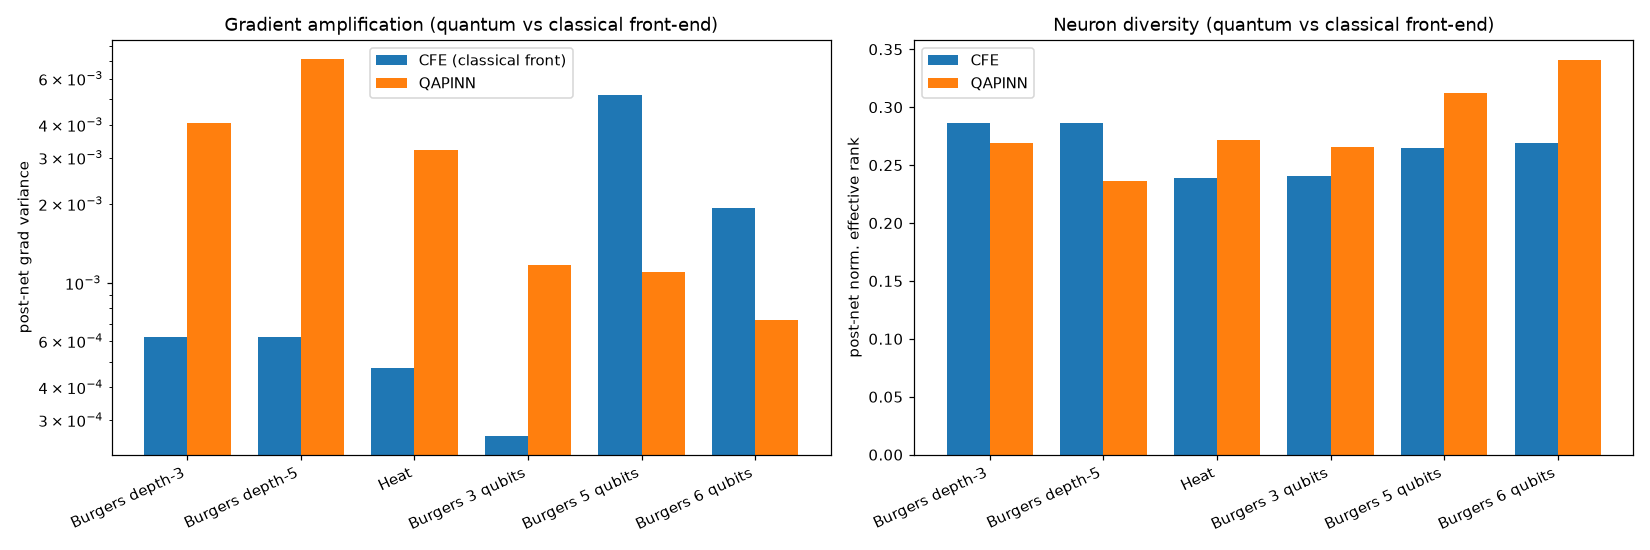
\includegraphics[width=\textwidth]{ablation_summary/cfe_comparison.png}
\caption{\textbf{The fair control, read directly.} Left --- post-net gradient variance: QAPINN (orange) exceeds the classical front-end (blue) at depth-3, depth-5, heat and 3 qubits, but the bars \emph{cross} at 5 and 6 qubits, where the classical control is now higher. The QAPINN's own gradient variance falls monotonically along the qubit axis (4q $\approx$ 4e-3 $\to$ 5q $\approx$ 1.1e-3 $\to$ 6q $\approx$ 7e-4, a $\sim$6$\times$ drop). Right --- neuron effective rank: the classical front-end is \emph{more} diverse on the depth axis, the QAPINN more diverse on the qubit axis --- no consistent winner.}
\end{figure}

\textbf{Observation.} Neither claimed mechanism survives as a clean effect. Gradient
``amplification'' is real only at low qubit count and \emph{inverts} by 5--6 qubits;
neuron ``diversification'' has no consistent sign against the fair control.

\textbf{Inference.} The monotone fall of the QAPINN's gradient variance as qubits grow
(4$\to$6) --- while the equal-width classical control holds roughly flat --- is the textbook
fingerprint of a \textbf{barren plateau} opening as the Hilbert space enlarges. So the
qubit axis carries two \emph{opposing} effects at once: more band (helps accuracy) and
vanishing gradients (hurts trainability). That tension, not a monotone ``more qubits =
better'', is the honest picture --- and it is exactly why a design methodology must trade
band against trainability rather than maximise either. The earlier ``$2\times$ diversity /
$4\times$ gradients'' story was an \emph{attribution error}: the plain-PINN control differed
from the QAPINN in two ways at once (front end \emph{and} architecture), so it credited to
``quantum'' what was partly just ``different network''. The CFE isolates the front end, and
the effect dissolves. Building the right control was worth more than any single number it
produced.

\clearpage
\section{Convergence and seeds --- the statistics}
\textbf{Convergence (single seed):}
\begin{center}\small\begin{tabular}{lcc}\toprule
 & 2000 iters & 8000 iters \\ \midrule
QAPINN entanglement=none & 0.456 & \textbf{0.261} \\
QAPINN entanglement=linear & 0.472 & 0.437 \\
classical (121p) & 0.535 & 0.376 \\
\bottomrule\end{tabular}\end{center}
\textbf{Seeds (7 seeds, 2000 iters):}
\begin{center}\small\begin{tabular}{lc}\toprule
entanglement & rel-$L_2$ (mean $\pm$ std) \\ \midrule
none & 0.459 $\pm$ 0.011 \\ linear & 0.448 $\pm$ 0.022 \\
ring & 0.474 $\pm$ 0.014 \\ all-to-all & 0.462 $\pm$ 0.014 \\
\bottomrule\end{tabular}\quad (spread 0.026 $<$ 2$\times$std 0.030)\end{center}
\verdict{Entanglement is NOT significant at 2000 iters (7 seeds).} The single-seed
``entanglement doesn't help'' was noise at that budget. \emph{However}, at
\emph{convergence} (8000 iters, single seed) a large effect appears: entanglement=none
(0.261) beats classical while entanglement=linear (0.437) loses. So the effect, if real,
is \emph{training-dependent} and currently rests on one seed at convergence --- an
\textbf{open lead}, not a claim. Convergence itself matters: 4$\times$ training reorders
the models.

\textbf{Inference.} The reordering under longer training is a methodological warning with
teeth: at 2000 iterations the classical control is \emph{worst} of the three (0.535); at
8000 it is \emph{best-but-one} (0.376), overtaking the entangled QAPINN. A benchmark that
stopped at 2000 iterations --- as many in the literature effectively do --- would have
reported the opposite ranking to the converged one. This is precisely how non-converged,
single-budget comparisons manufacture ``quantum advantage'' (or erase it): the models sit
at different points on their loss curves, and whoever is compared mid-descent wins by
accident. Our takeaway is not the 8000-iter numbers themselves (one seed) but the
structural point --- \emph{any} accuracy claim without a convergence check and error bars is
a claim about training budget, not about the model.

\textbf{Observation (from the 8000-iter figures).} Reading the three converged runs
side by side makes the entanglement lead vivid, not just numeric. The
\emph{no-entanglement} QAPINN (\texttt{conv\_qapinn\_entnone}, entropy $\sim$10$^{-7}$)
develops a genuinely \emph{crisp} shock: a near-vertical transition at $x=0$ whose
residual is a razor-thin line, and a realized spectrum that matches the reference
\emph{bar-for-bar out to $k=20$} --- the high-$k$ coefficients are $\sim$2, versus
$\sim$0.04 for the entangled run. The \emph{entangled} QAPINN
(\texttt{conv\_qapinn\_base}) carries real, structured entanglement ($S\sim0.5$--$1.1$)
yet, even at 4$\times$ training, keeps a smooth ramp (peak $\sim$0.65) and a band-limited
spectrum. The classical net (\texttt{conv\_cls\_121}) also sharpens the shock (peak
$\sim$0.78) but with visible Gibbs ringing.

\textbf{Inference.} At convergence the ordering is \emph{no-entanglement QAPINN}
$\approx$ \emph{classical} $\gg$ \emph{entangled QAPINN} on the very thing that matters
here --- high-frequency shock content. So the entangling layers are not neutral at this
budget; they appear to \emph{cost} high-$k$ expressivity, plausibly by tangling the
optimization (the barren-plateau tendency seen on the qubit axis). This is the study's
sharpest open lead: it says the field's default ``add entanglement for expressibility''
instinct can be exactly backwards for stiff, high-frequency PDE targets. It rests on one
seed at convergence and must be repeated across seeds before it is a claim --- but it is
now a lead grounded in a spectrum you can read, not a single scalar.

\clearpage
\section{The $\nu$-sweep --- bandwidth sufficiency}
\textbf{Hypothesis.} If bandwidth is a \emph{sufficient statistic} for advantage, then
tuning $\nu$ (which continuously changes solution bandwidth) plus the heat point should
collapse the advantage onto one curve of advantage-vs-bandwidth. The $\nu\to$bandwidth
map is already verified ($\nu{=}0.1{\to}$bw 3, $\nu{=}0.003{\to}$bw 22, heat$\to$1), and
is itself the core of the design methodology: cheap physics proxy $\to$ bandwidth $\to$
depth.

\textbf{Observation (from the completed, corrected sweep).} Both models' error rises
\emph{monotonically} with solution bandwidth --- but the \emph{advantage} does not collapse
onto a clean curve. The full table (heat is the bandwidth-1 anchor; ``base'' is the
original $\nu=0.01/\pi$):
\begin{center}\small\begin{tabular}{lcccccc}\toprule
label & heat & $\nu{=}0.1$ & $\nu{=}0.05$ & $\nu{=}0.02$ & $\nu{=}0.01$ & base \\
solution bandwidth & 1 & 3 & 5 & 10 & 15 & 22 \\ \midrule
classical rel-$L_2$ & 0.008 & 0.018 & 0.032 & 0.069 & 0.141 & 0.535 \\
QAPINN (depth 3) rel-$L_2$ & 0.006 & 0.049 & 0.077 & 0.165 & 0.354 & 0.472 \\
advantage (cls$-$QAP) & $+$0.00 & $-$0.03 & $-$0.05 & $-$0.10 & $-$0.21 & $+$0.06 \\
\bottomrule\end{tabular}\end{center}
\begin{figure}[H]\centering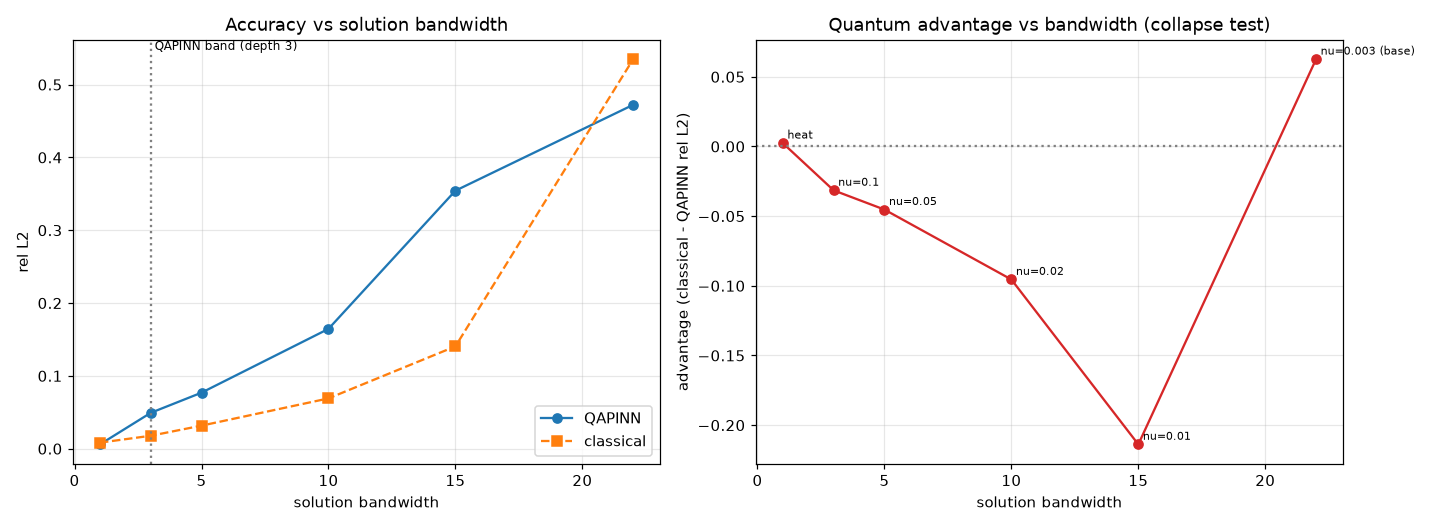
\includegraphics[width=\textwidth]{ablation_summary/nusweep.png}
\caption{\textbf{The collapse test.} Left: both curves rise with bandwidth; the matched
classical (orange) is \emph{below} (better than) the depth-3 QAPINN (blue) everywhere up
to bandwidth $\sim$15, then the two \emph{cross} near bandwidth 20. Right: the advantage
is \textbf{V-shaped} --- near zero at heat, going negative (QAPINN worse) and bottoming at
$-0.21$ at bandwidth 15, then flipping positive ($+0.06$) only at the extreme bandwidth 22
where \emph{both} models are failing ($\sim$0.5).}\end{figure}
\textbf{Inference.} \verdict{The sufficiency hypothesis is not confirmed.} Bandwidth
cleanly predicts each model's \emph{error} (both curves are monotone), but it does
\emph{not} collapse the \emph{advantage} onto a single function --- the sign of the
advantage is regime-dependent. For the fixed depth-3 band the QAPINN \emph{loses} to its
matched classical control across almost the whole family (advantage negative from
bandwidth 3 to 15), worst exactly where the band is most out-run (bandwidth 15), and only
edges ahead at bandwidth 22 where both models have essentially failed and the Fourier
prior degrades slightly more gracefully. This is a genuine (and honest) deflation of the
neat ``bandwidth is a sufficient statistic'' story: bandwidth is the right \emph{axis} for
error, but advantage also depends on how the band compares to the target and on
which model breaks first. The usable methodology lesson survives in a weaker,
truer form --- $\nu$ (or Reynolds number, or a coarse solve) is a cheap proxy for the
\emph{band you must cover}, and if you cannot cover it, the quantum layer is not a
substitute for the missing depth.

\textbf{A bug we caught doing this.} While inspecting every figure we found that the
per-run \emph{solution} plots for the $\nu$-sweep had been drawn against the
\emph{default}-viscosity reference (the figure code called \texttt{get\_pde(pde)} without
the run's \texttt{pde\_params}), even though the reported rel-$L_2$ used the correct
per-$\nu$ reference. The smooth-$\nu$ runs therefore \emph{looked} like bad fits against a
sharp reference they were never trained on. We fixed the one-line defect in
\texttt{run.py} and regenerated the affected figures (now shown); the numbers above were
always correct. It is a small bug, but a clean illustration of why we read every figure
rather than trusting the montage.

\emph{The collapse plot (\texttt{results/ablation\_summary/nusweep.png}) populates on
\texttt{run\_nusweep.py aggregate} once the last QAPINN point finishes.}

\clearpage
\section{What survived vs what deflated (honest summary)}
\begin{center}\small\begin{tabular}{lll}\toprule
Finding & Status & Why \\ \midrule
Depth/qubits/scale help (bandwidth) & \textbf{robust} & monotonic, physically grounded, verified \\
VQC $=$ Fourier, band $=$ depth & \textbf{robust} & proven [1] + verified on our code \\
input\_scale $2\pi$ collapse & \textbf{robust} & clean; reproduces the black-hole pathology \\
Barren-plateau in qubit count & \textbf{plausible} & grad-var shrinks with qubits (CFE) \\
Advantage bandwidth-gated & \textbf{plausible} & fair control ties at low bandwidth \\
Entanglement doesn't help & \verdict{not sig.\ @2000i} & within 7-seed noise \\
Entanglement harmful @convergence & \emph{open lead} & large effect, single seed \\
Quantum diversifies classical neurons & \verdict{refuted} & died under the fair CFE control \\
2$\times$ diversity / 4$\times$ gradients & \verdict{artifact} & mismatched plain-PINN control \\
Capacity (not band) fixes the shock & \verdict{refuted} & classical error non-monotonic in params \\
Error rises monotonically with bandwidth ($\nu$) & \textbf{robust} & clean curve, both models \\
Depth-3 QAPINN beats classical on $\nu$-sweep & \verdict{no} & ties/loses at every $\nu$ (band too low) \\
\bottomrule\end{tabular}\end{center}
\textbf{Methodological contributions (independent of the findings):} a \emph{verified}
(8/8) pipeline; \emph{matched-parameter} and \emph{structurally-matched} controls;
\emph{multi-seed} statistics; full reproducibility. Most of the QAPINN literature has
none of these.

\clearpage
\part*{Part II --- Complete run gallery (all 77 runs, every figure)}
\addcontentsline{toc}{section}{Part II --- Complete run gallery}
Every training run in \texttt{results/}, with its metadata and \emph{all} of its
per-run figures at full width. Nothing curated out. Figure order per run: solution,
spectrum, F-principle, neurons, per-qubit $\langle Z\rangle$, entanglement, landscape,
generalization, evolution, loss (whichever exist for that model).

\section{Reference run --- abl\_baseline (the canonical QAPINN)}
The depth-3, 4-qubit, linear-entanglement, multi-$Z$, scale-1 configuration that every
Tier-1/Tier-3 sweep varies one knob from, and the reference point in the ablation
tables.

\subsection{abl\_baseline}
\noindent\small \textbf{rel-$L_2$}: 0.4722  \textbf{params}: 121  \textbf{PDE}: burgers  \textbf{Adam iters}: 2000  \textbf{seed}: 0  \textbf{model}: qapinn  \textbf{final PDE loss}: 3.85e-02  \textbf{wall time (s)}: 1684  \textbf{VQC}: 4q x3L ent=linear meas=multi scale=1.0\normalsize

\noindent\textbf{Observation.} Identical to burgers\_qapinn (same figures): smeared shock, amplitude capped \textasciitilde{}0.65, |error| bowtie about x=0 peaking \textasciitilde{}0.9. Spectrum matches k=1-2 then falls below the reference from k\textasciitilde{}3, \textasciitilde{}1.5 decades low by k=20. Entanglement S spans \textasciitilde{}0.45 to \textasciitilde{}1.05 with the bright corner at bottom-left (x\textless{}-0.5, t\textless{}0.2) and a dark band near x=0; qubit 0 shows the strong horizontal x-band. Inference: this is the reference depth configuration and it sits at the moderate-entanglement, shock-limited operating point that the depth ablations vary around.

\begin{figure}[H]\centering
\includegraphics[width=\textwidth]{abl_baseline/figures/solution.png}
\caption{\textbf{abl\_baseline} --- Predicted field $u(x,t)$ vs.\ exact reference, with the pointwise error map. The shock ($x\!=\!0$) is where a smooth network struggles.}
\end{figure}
\begin{figure}[H]\centering
\includegraphics[width=\textwidth]{abl_baseline/figures/spectrum.png}
\caption{\textbf{abl\_baseline} --- Realized spatial spectrum (per-harmonic magnitude) vs.\ reference. Tests whether the model captures the high-$k$ shock tail or only low frequencies.}
\end{figure}
\begin{figure}[H]\centering
\includegraphics[width=\textwidth]{abl_baseline/figures/fprinciple.png}
\caption{\textbf{abl\_baseline} --- F-principle heat-map: iteration at which each harmonic's relative error halves. Low harmonics converging first is the F-principle signature.}
\end{figure}
\begin{figure}[H]\centering
\includegraphics[width=\textwidth]{abl_baseline/figures/neurons.png}
\caption{\textbf{abl\_baseline} --- Classical post-net neurons: receptive fields over $(x,t)$ and each neuron's dominant spatial frequency / effective rank.}
\end{figure}
\begin{figure}[H]\centering
\includegraphics[width=\textwidth]{abl_baseline/figures/qubits.png}
\caption{\textbf{abl\_baseline} --- Per-qubit $\langle Z\rangle$ receptive fields --- what feature each qubit computes over the domain (quantum models only).}
\end{figure}
\begin{figure}[H]\centering
\includegraphics[width=\textwidth]{abl_baseline/figures/entanglement.png}
\caption{\textbf{abl\_baseline} --- Von Neumann entanglement entropy $S(x,t)$ of a qubit bipartition across the domain (quantum models only).}
\end{figure}
\begin{figure}[H]\centering
\includegraphics[width=\textwidth]{abl_baseline/figures/landscape.png}
\caption{\textbf{abl\_baseline} --- Filter-normalized 2-D loss landscape around the trained minimum (Li et al.\ 2018). Flat/wide vs.\ sharp basin.}
\end{figure}
\begin{figure}[H]\centering
\includegraphics[width=\textwidth]{abl_baseline/figures/generalization.png}
\caption{\textbf{abl\_baseline} --- Extrapolation: relative $L_2$ vs.\ $t$ beyond the $t\in[0,1]$ training window --- the off-domain penalty.}
\end{figure}
\begin{figure}[H]\centering
\includegraphics[width=\textwidth]{abl_baseline/figures/loss.png}
\caption{\textbf{abl\_baseline} --- Training loss history (total, PDE-residual, and constraint terms).}
\end{figure}
\clearpage
\section{Base comparison --- heat \& Burgers, classical vs.\ QAPINN}
Four runs at matched 121 parameters, identical training. The clean spectral contrast: heat stays a single Fourier mode, Burgers spreads to high harmonics.

\subsection{heat\_classical}
\noindent\small \textbf{rel-$L_2$}: 0.0083  \textbf{params}: 121  \textbf{PDE}: heat  \textbf{Adam iters}: 2000  \textbf{seed}: 0  \textbf{model}: classical  \textbf{final PDE loss}: 3.21e-04  \textbf{wall time (s)}: 19\normalsize

\noindent\textbf{Observation.} Prediction matches the reference diffusion field almost exactly; the t=0.25/0.50/0.75 snapshots show the red model dashes sitting on top of the black reference with no visible amplitude cap (peaks \textasciitilde{}0.8, 0.6, 0.47 all reproduced). |error| stays under \textasciitilde{}0.021 and is concentrated in thin bands at the top and bottom edges near x=+/-0.75 to +/-1.0 (worst spot lower-left near t=0, x=-0.8). The Fourier spectrum tracks the reference bar-for-bar all the way to k=20 with only tiny per-harmonic deviations, and the only mismatch is k=0 where the model shows a small \textasciitilde{}0.1 offset vs the reference near-zero mean. Inference: a smooth low-frequency heat solution is fit essentially perfectly by the classical PINN with no spectral-bias cutoff.

\begin{figure}[H]\centering
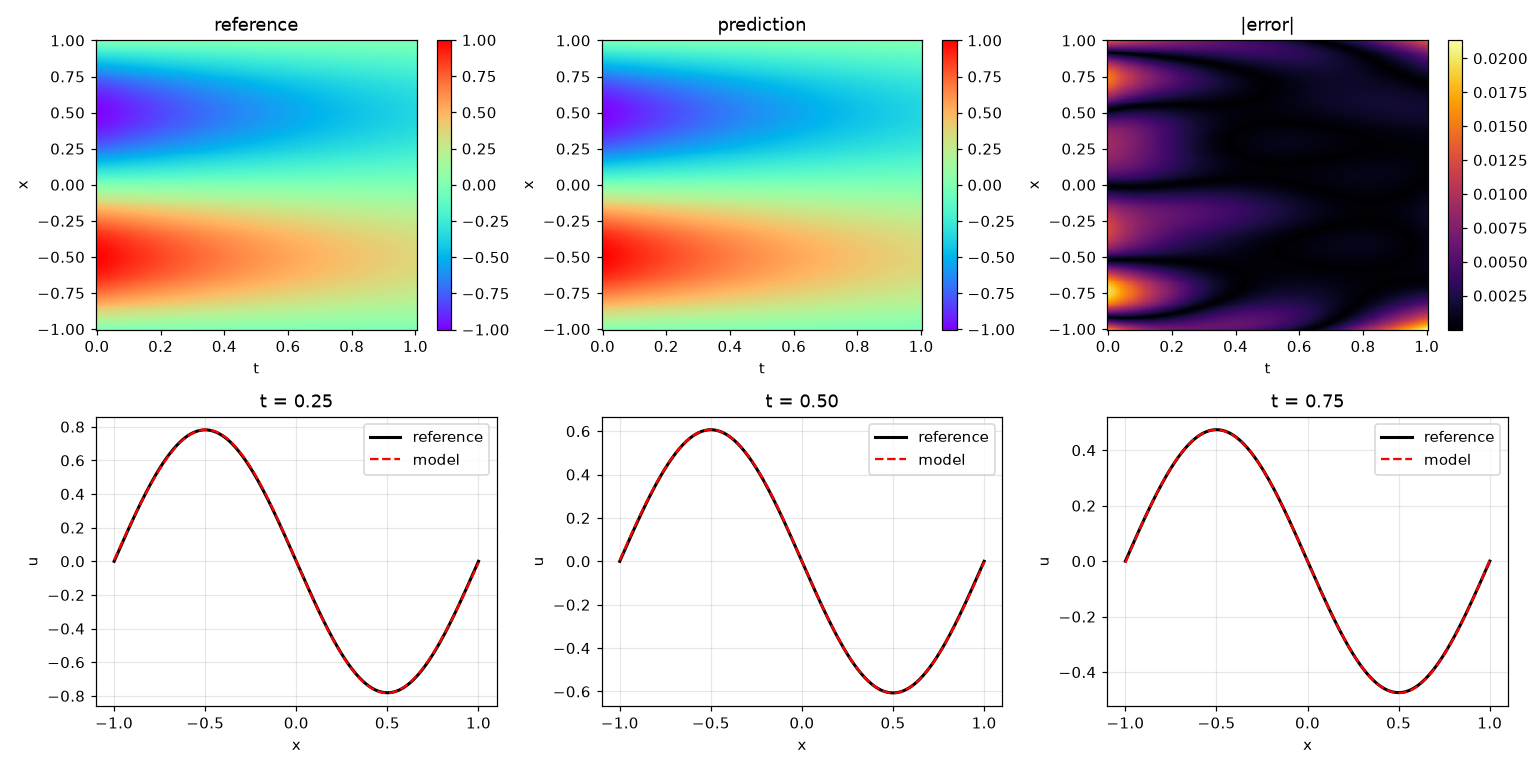
\includegraphics[width=\textwidth]{heat_classical/figures/solution.png}
\caption{\textbf{heat\_classical} --- Predicted field $u(x,t)$ vs.\ exact reference, with the pointwise error map. The shock ($x\!=\!0$) is where a smooth network struggles.}
\end{figure}
\begin{figure}[H]\centering
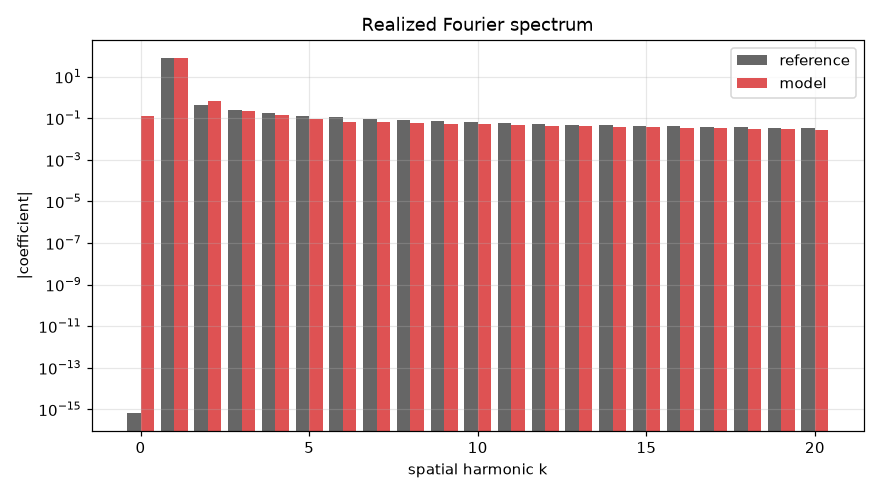
\includegraphics[width=\textwidth]{heat_classical/figures/spectrum.png}
\caption{\textbf{heat\_classical} --- Realized spatial spectrum (per-harmonic magnitude) vs.\ reference. Tests whether the model captures the high-$k$ shock tail or only low frequencies.}
\end{figure}
\begin{figure}[H]\centering
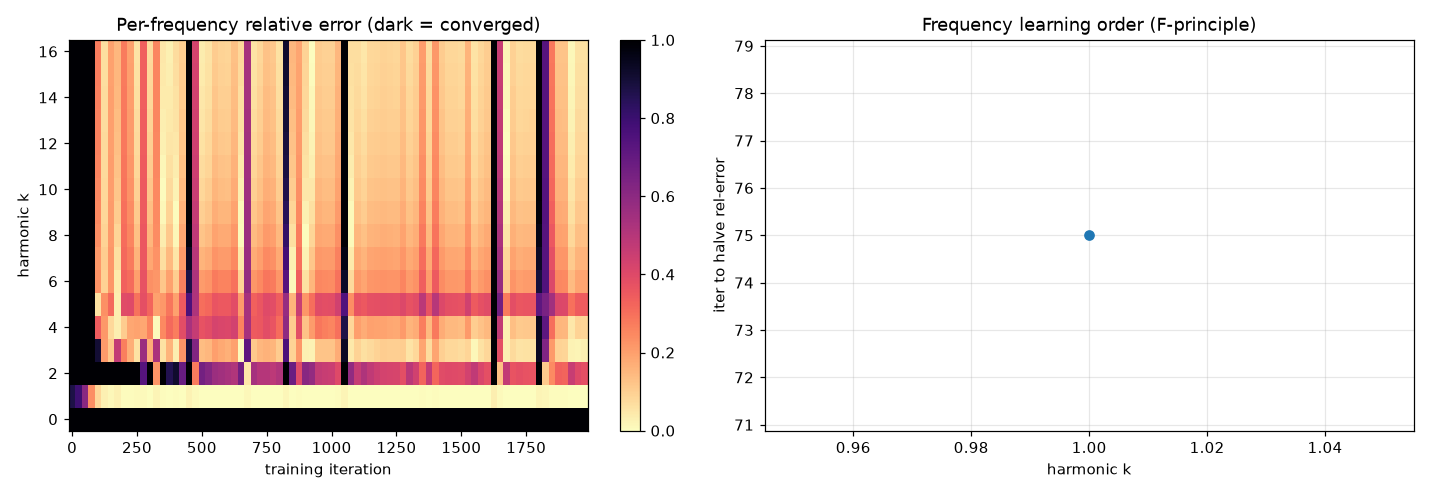
\includegraphics[width=\textwidth]{heat_classical/figures/fprinciple.png}
\caption{\textbf{heat\_classical} --- F-principle heat-map: iteration at which each harmonic's relative error halves. Low harmonics converging first is the F-principle signature.}
\end{figure}
\begin{figure}[H]\centering
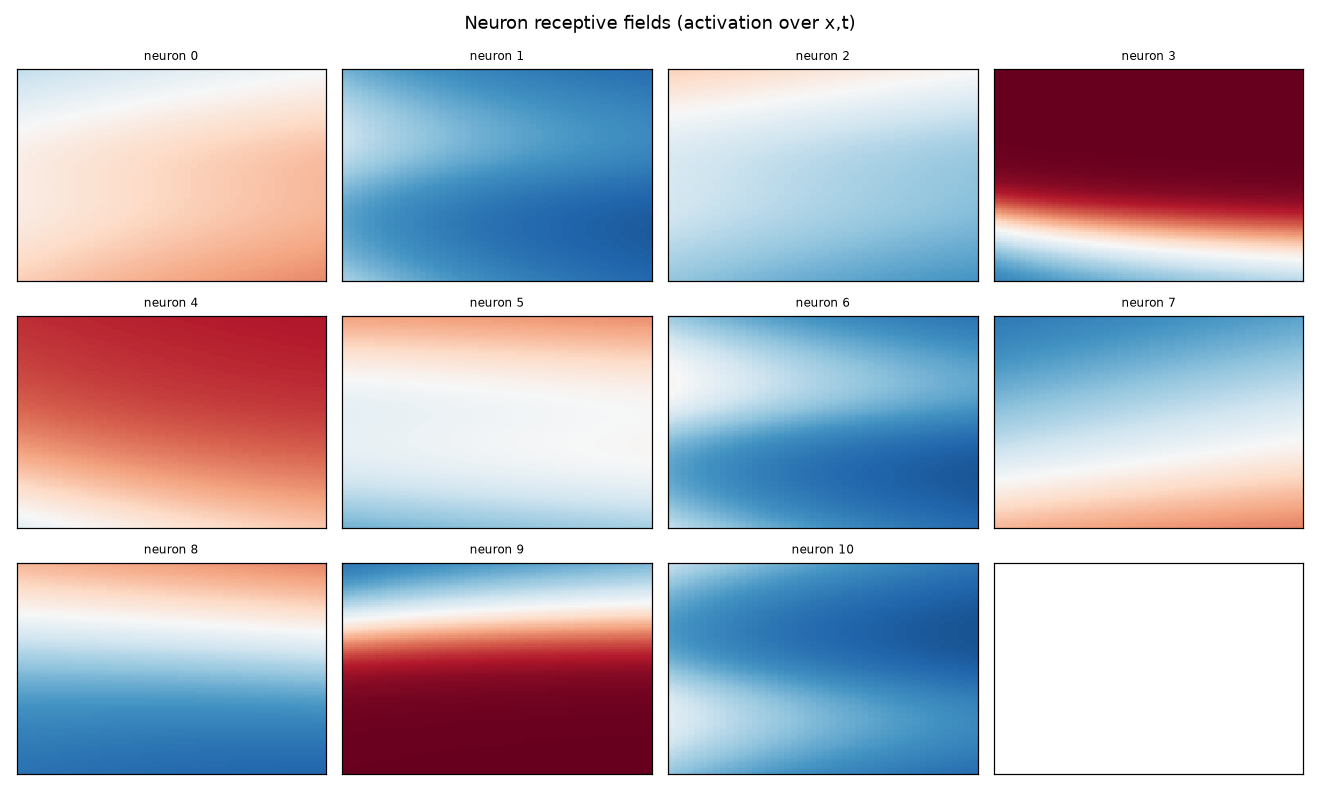
\includegraphics[width=\textwidth]{heat_classical/figures/neurons.png}
\caption{\textbf{heat\_classical} --- Classical post-net neurons: receptive fields over $(x,t)$ and each neuron's dominant spatial frequency / effective rank.}
\end{figure}
\begin{figure}[H]\centering
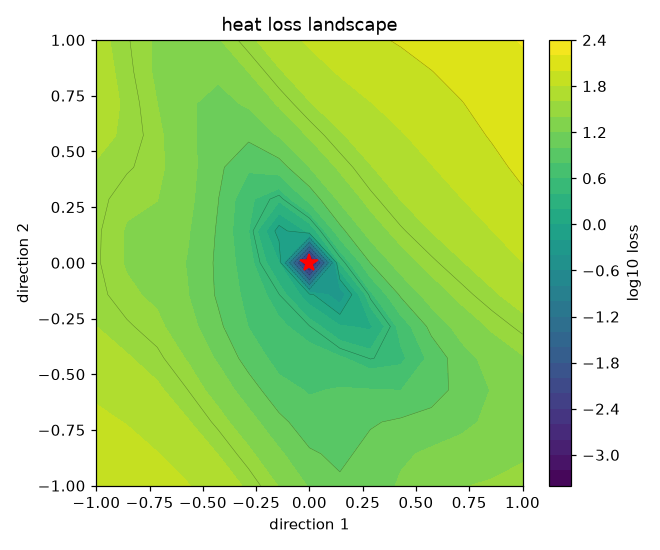
\includegraphics[width=\textwidth]{heat_classical/figures/landscape.png}
\caption{\textbf{heat\_classical} --- Filter-normalized 2-D loss landscape around the trained minimum (Li et al.\ 2018). Flat/wide vs.\ sharp basin.}
\end{figure}
\begin{figure}[H]\centering
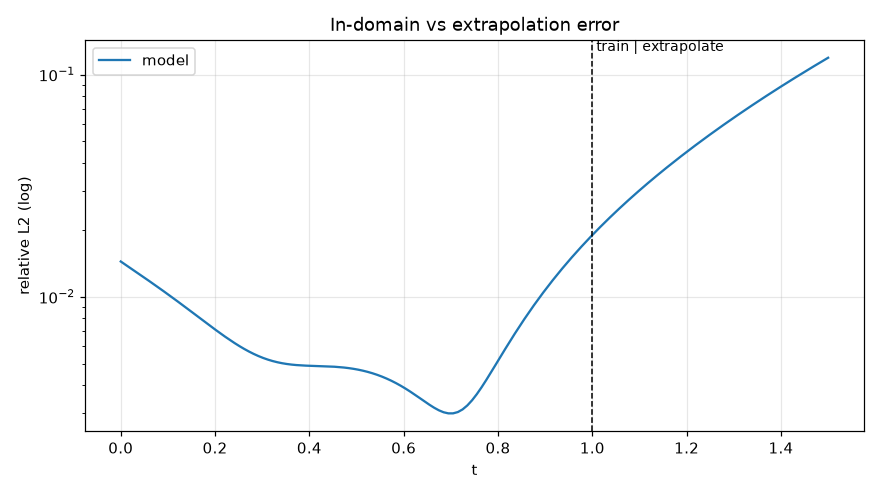
\includegraphics[width=\textwidth]{heat_classical/figures/generalization.png}
\caption{\textbf{heat\_classical} --- Extrapolation: relative $L_2$ vs.\ $t$ beyond the $t\in[0,1]$ training window --- the off-domain penalty.}
\end{figure}
\begin{figure}[H]\centering
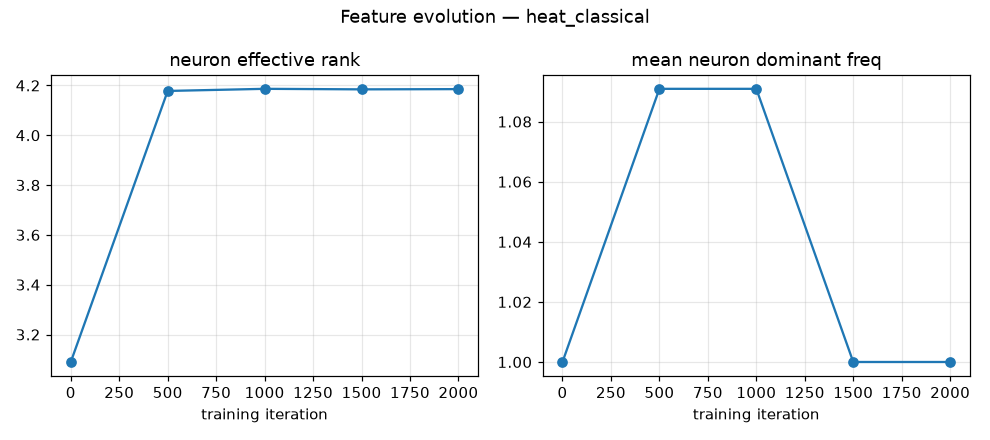
\includegraphics[width=\textwidth]{heat_classical/figures/evolution.png}
\caption{\textbf{heat\_classical} --- Solution evolution: snapshots of $u(x,\cdot)$ across time.}
\end{figure}
\begin{figure}[H]\centering
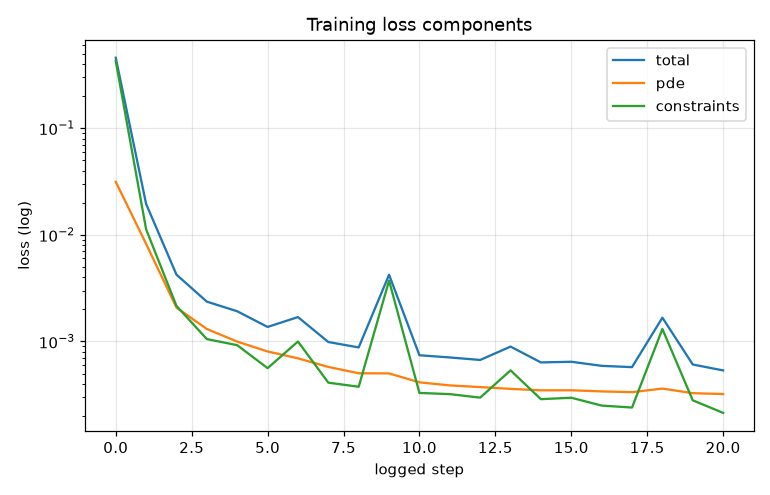
\includegraphics[width=\textwidth]{heat_classical/figures/loss.png}
\caption{\textbf{heat\_classical} --- Training loss history (total, PDE-residual, and constraint terms).}
\end{figure}
\clearpage
\subsection{heat\_qapinn}
\noindent\small \textbf{rel-$L_2$}: 0.0059  \textbf{params}: 121  \textbf{PDE}: heat  \textbf{Adam iters}: 2000  \textbf{seed}: 0  \textbf{model}: qapinn  \textbf{final PDE loss}: 2.21e-04  \textbf{wall time (s)}: 2107  \textbf{VQC}: 4q x3L ent=linear meas=multi scale=1.0\normalsize

\noindent\textbf{Observation.} Quantum model reproduces the smooth heat field well; snapshot dashes overlie the reference with only a hair of amplitude softening (prediction colorbar tops \textasciitilde{}0.86 vs reference 1.0 at the t=0 initial peak). |error| peaks \textasciitilde{}0.013 (lower than the classical run's 0.02) and forms swirled patches on the left edge near t=0, strongest around x=-0.85. Spectrum matches the reference through k=20 with a spurious k=0 bar (\textasciitilde{}0.1) as the only real defect. Entanglement S(x,t) is smooth, ranging \textasciitilde{}0.35 (dark trough near x=0.1, t=0.1) to \textasciitilde{}1.2 (bright upper-right, x\textgreater{}0.5 and t\textgreater{}0.5), and the four \textless{}Z\textgreater{} qubit maps are clean low-frequency receptive fields (qubit 0 a strong horizontal x-band). Inference: on an easy smooth problem the QAPINN matches or slightly beats the classical PINN while using low, spatially-structured entanglement.

\begin{figure}[H]\centering
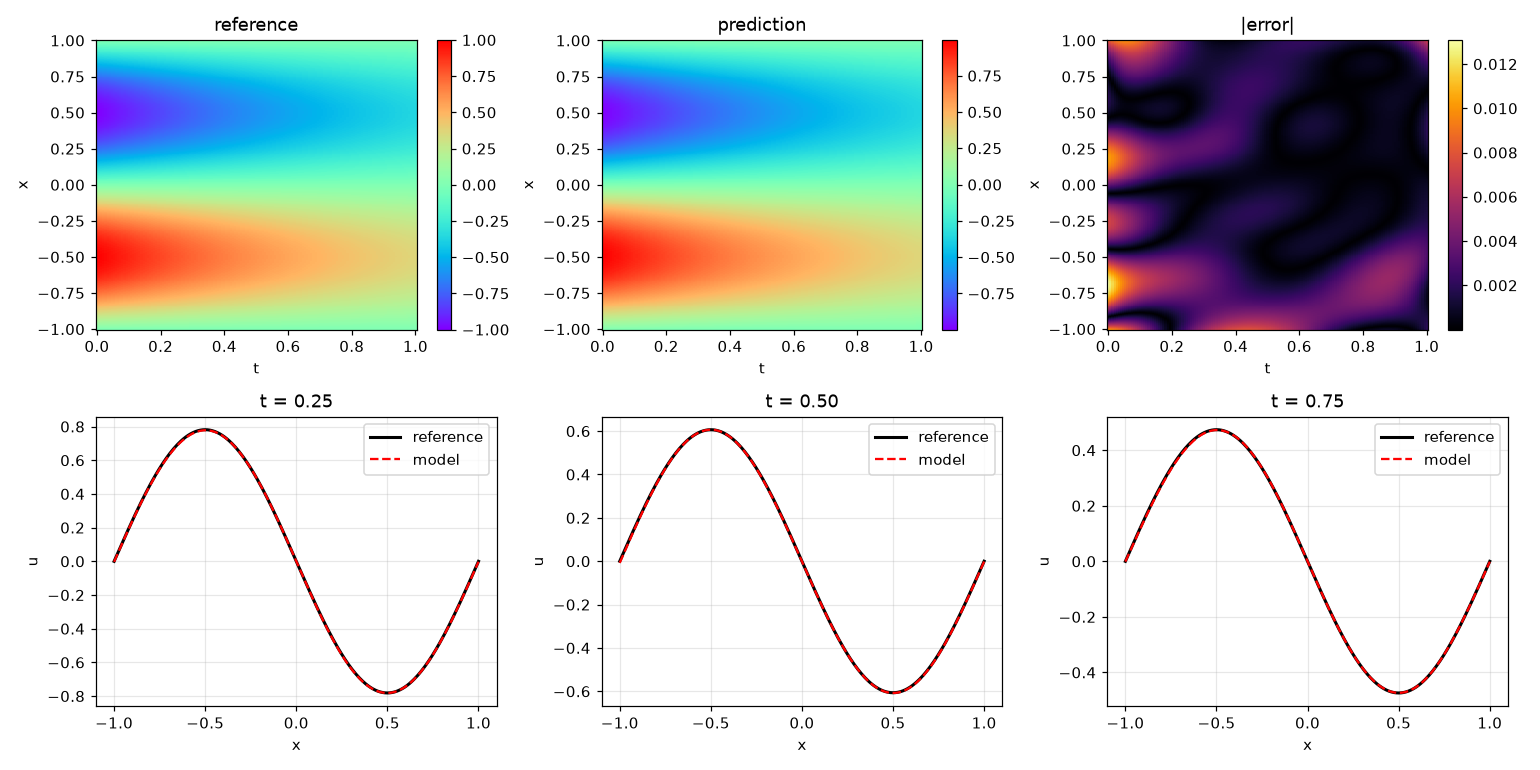
\includegraphics[width=\textwidth]{heat_qapinn/figures/solution.png}
\caption{\textbf{heat\_qapinn} --- Predicted field $u(x,t)$ vs.\ exact reference, with the pointwise error map. The shock ($x\!=\!0$) is where a smooth network struggles.}
\end{figure}
\begin{figure}[H]\centering
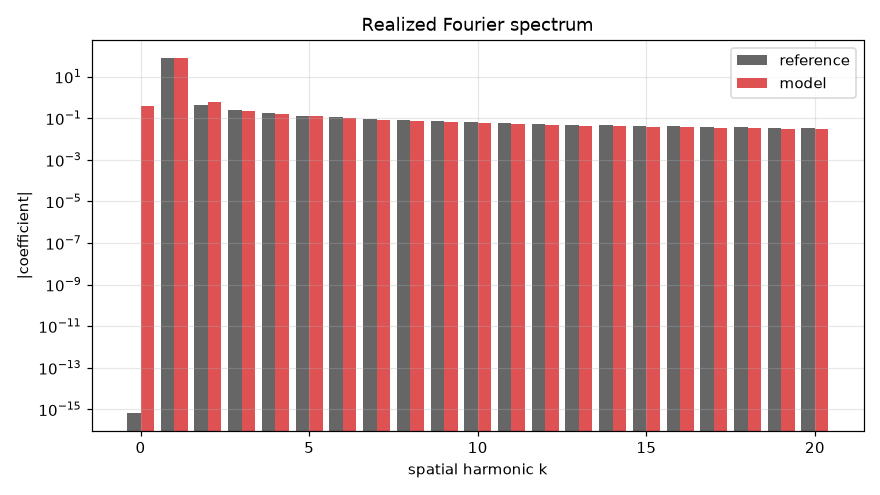
\includegraphics[width=\textwidth]{heat_qapinn/figures/spectrum.png}
\caption{\textbf{heat\_qapinn} --- Realized spatial spectrum (per-harmonic magnitude) vs.\ reference. Tests whether the model captures the high-$k$ shock tail or only low frequencies.}
\end{figure}
\begin{figure}[H]\centering
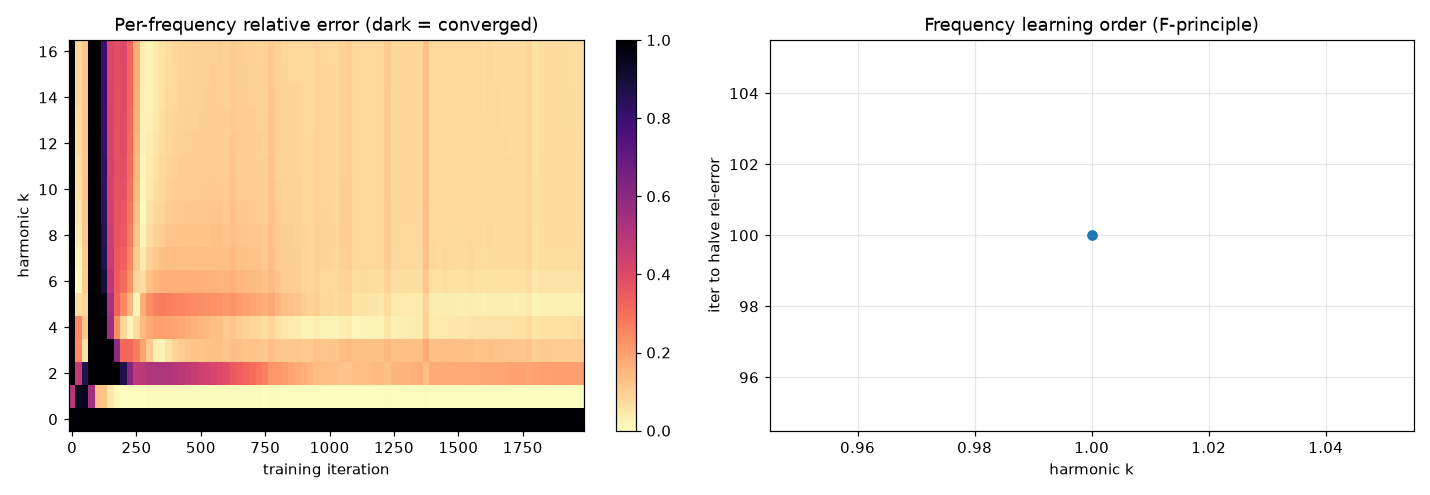
\includegraphics[width=\textwidth]{heat_qapinn/figures/fprinciple.png}
\caption{\textbf{heat\_qapinn} --- F-principle heat-map: iteration at which each harmonic's relative error halves. Low harmonics converging first is the F-principle signature.}
\end{figure}
\begin{figure}[H]\centering
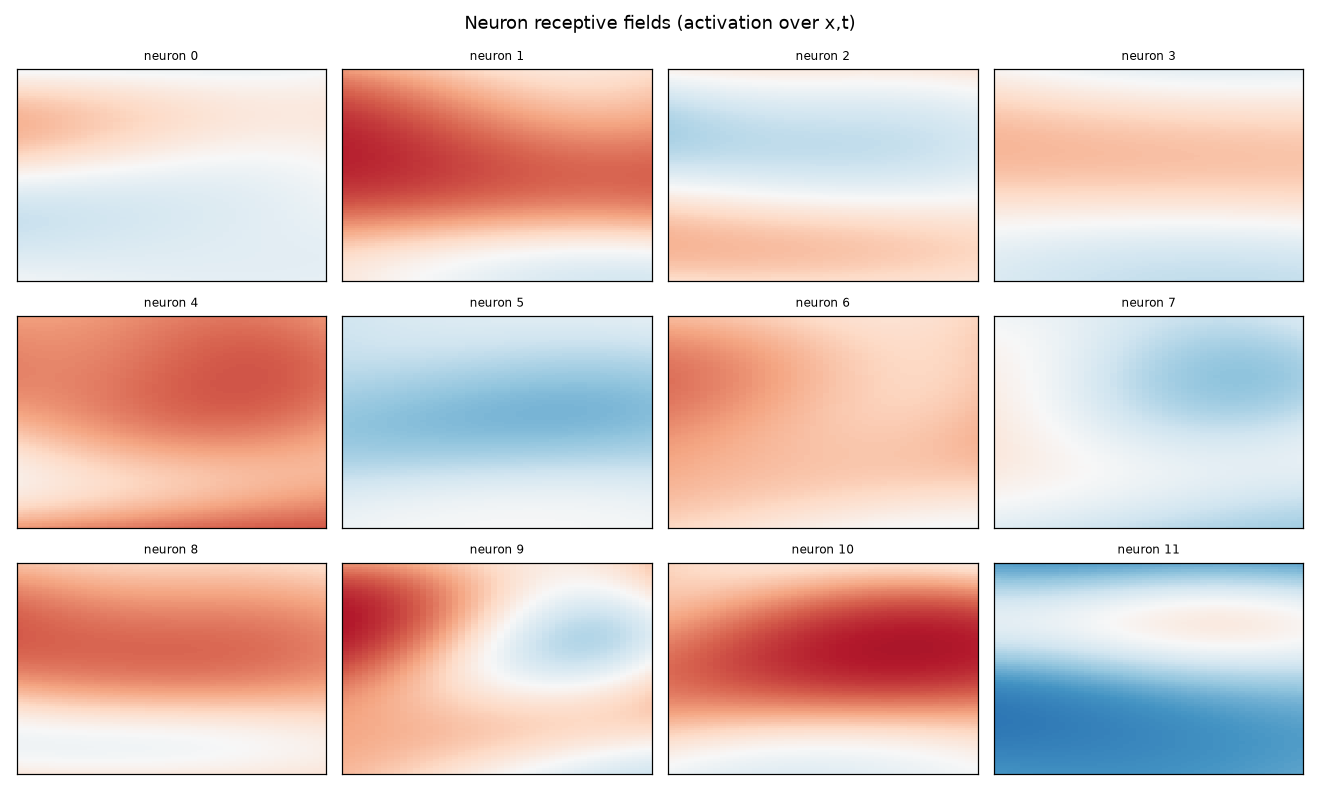
\includegraphics[width=\textwidth]{heat_qapinn/figures/neurons.png}
\caption{\textbf{heat\_qapinn} --- Classical post-net neurons: receptive fields over $(x,t)$ and each neuron's dominant spatial frequency / effective rank.}
\end{figure}
\begin{figure}[H]\centering
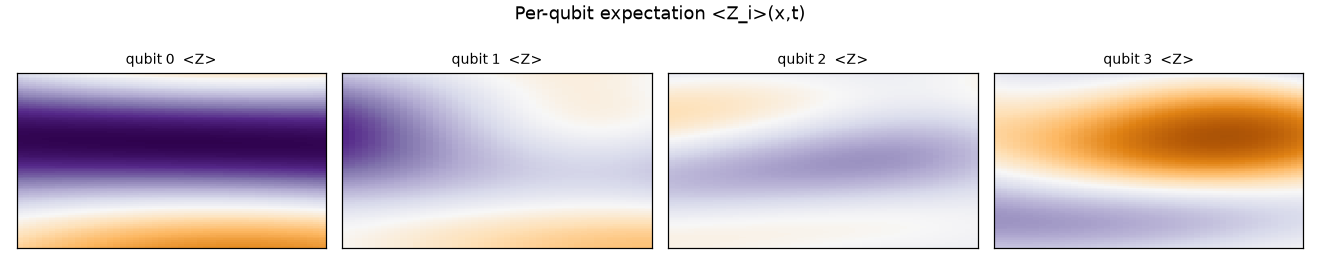
\includegraphics[width=\textwidth]{heat_qapinn/figures/qubits.png}
\caption{\textbf{heat\_qapinn} --- Per-qubit $\langle Z\rangle$ receptive fields --- what feature each qubit computes over the domain (quantum models only).}
\end{figure}
\begin{figure}[H]\centering
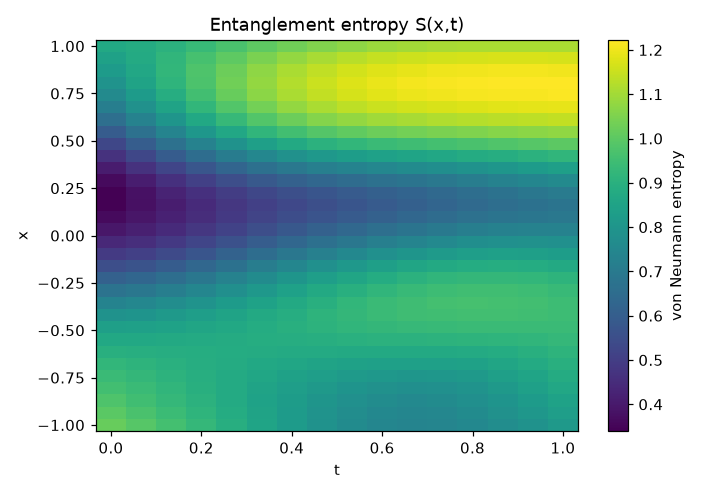
\includegraphics[width=\textwidth]{heat_qapinn/figures/entanglement.png}
\caption{\textbf{heat\_qapinn} --- Von Neumann entanglement entropy $S(x,t)$ of a qubit bipartition across the domain (quantum models only).}
\end{figure}
\begin{figure}[H]\centering
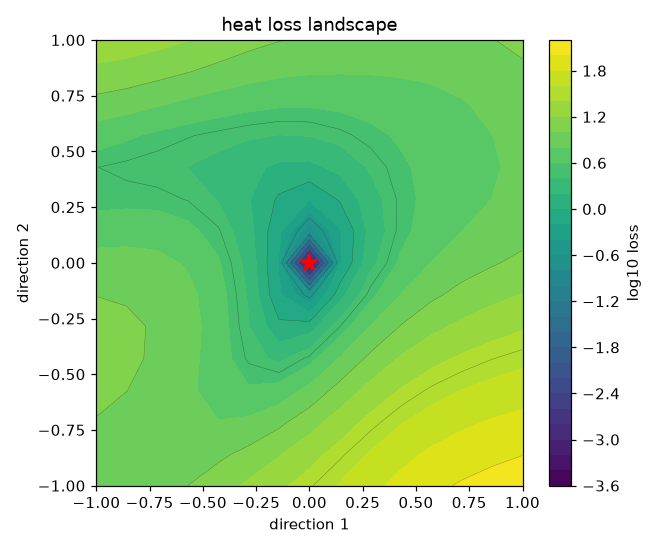
\includegraphics[width=\textwidth]{heat_qapinn/figures/landscape.png}
\caption{\textbf{heat\_qapinn} --- Filter-normalized 2-D loss landscape around the trained minimum (Li et al.\ 2018). Flat/wide vs.\ sharp basin.}
\end{figure}
\begin{figure}[H]\centering
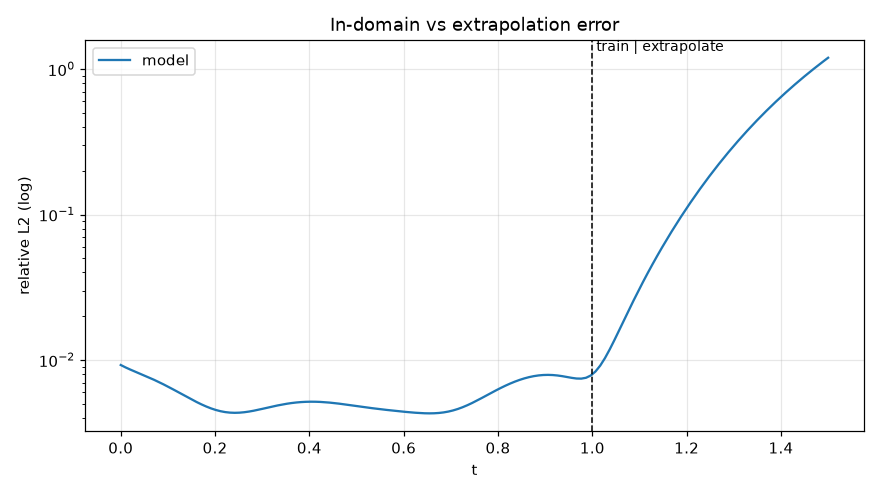
\includegraphics[width=\textwidth]{heat_qapinn/figures/generalization.png}
\caption{\textbf{heat\_qapinn} --- Extrapolation: relative $L_2$ vs.\ $t$ beyond the $t\in[0,1]$ training window --- the off-domain penalty.}
\end{figure}
\begin{figure}[H]\centering
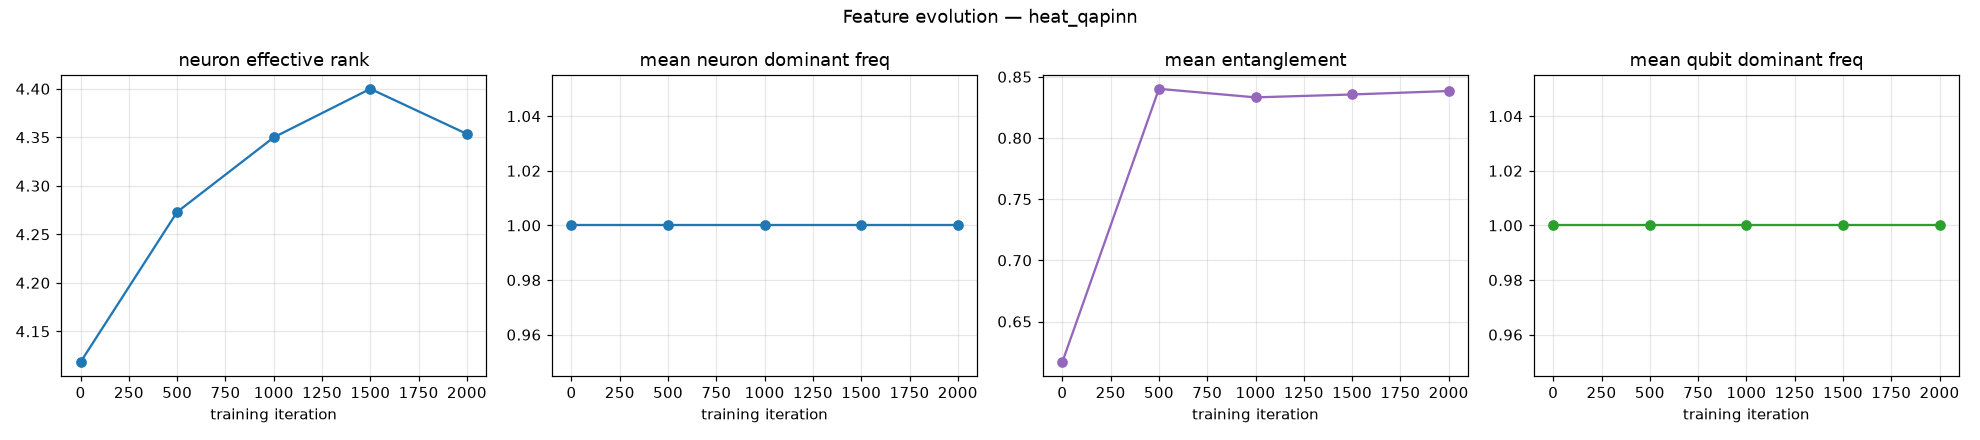
\includegraphics[width=\textwidth]{heat_qapinn/figures/evolution.png}
\caption{\textbf{heat\_qapinn} --- Solution evolution: snapshots of $u(x,\cdot)$ across time.}
\end{figure}
\begin{figure}[H]\centering
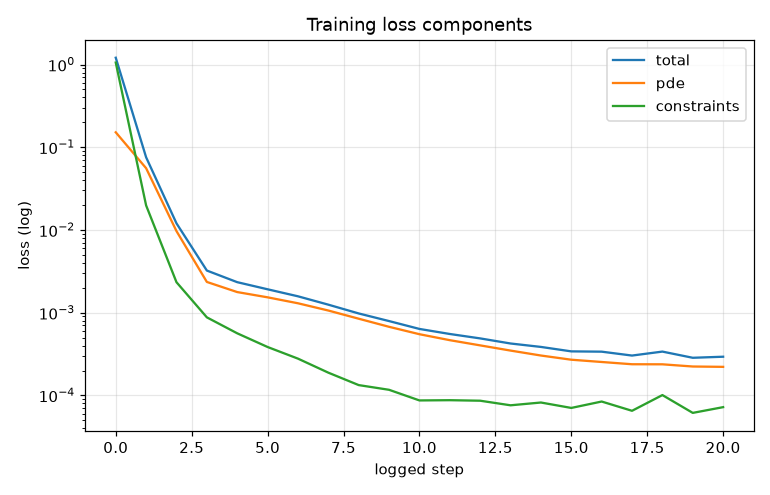
\includegraphics[width=\textwidth]{heat_qapinn/figures/loss.png}
\caption{\textbf{heat\_qapinn} --- Training loss history (total, PDE-residual, and constraint terms).}
\end{figure}
\clearpage
\subsection{burgers\_classical}
\noindent\small \textbf{rel-$L_2$}: 0.4326  \textbf{params}: 121  \textbf{PDE}: burgers  \textbf{Adam iters}: 2000  \textbf{seed}: 0  \textbf{model}: classical  \textbf{final PDE loss}: 2.99e-02  \textbf{wall time (s)}: 19\normalsize

\noindent\textbf{Observation.} The model completely fails to capture the Burgers shock at x=0: the prediction is a smooth sawtooth with amplitude capped at \textasciitilde{}0.7 (colorbar max \textasciitilde{}0.68) versus the reference's sharp +/-1.0 jump. Snapshots show the red model rounding off the steep gradient and undershooting both lobes (e.g. t=0.5 model peak \textasciitilde{}0.6 vs reference \textasciitilde{}1.0), and |error| forms a bright bowtie straddling x=0 that reaches \textasciitilde{}0.9. The spectrum matches only k=1-2, then the model falls progressively below the reference from k\textasciitilde{}3 onward, ending roughly 1.5-2 decades low by k=20 (model \textasciitilde{}1e-2 vs reference \textasciitilde{}1). Inference: classic spectral bias, the smooth network cannot represent the high-harmonic content of the discontinuity.

\begin{figure}[H]\centering
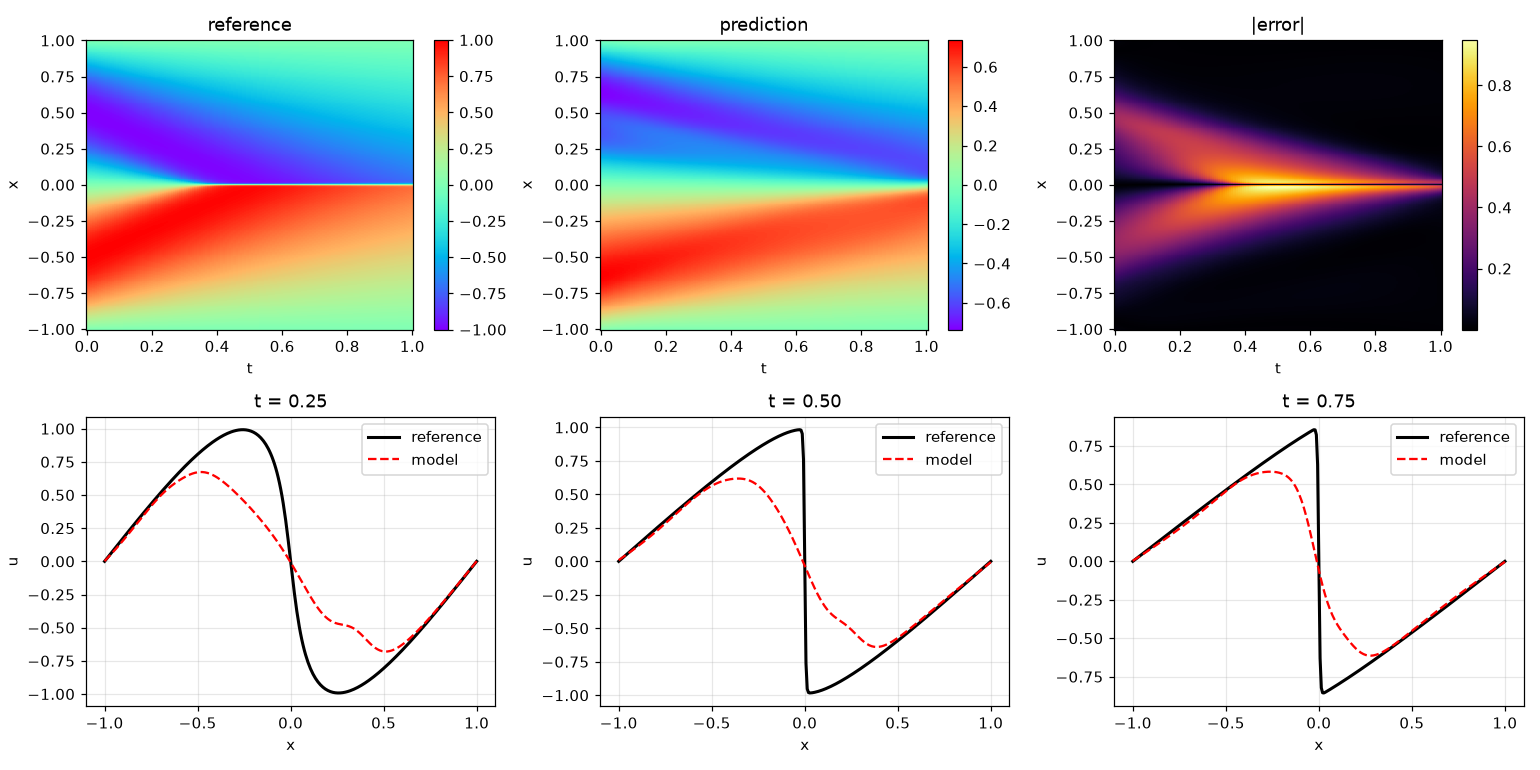
\includegraphics[width=\textwidth]{burgers_classical/figures/solution.png}
\caption{\textbf{burgers\_classical} --- Predicted field $u(x,t)$ vs.\ exact reference, with the pointwise error map. The shock ($x\!=\!0$) is where a smooth network struggles.}
\end{figure}
\begin{figure}[H]\centering
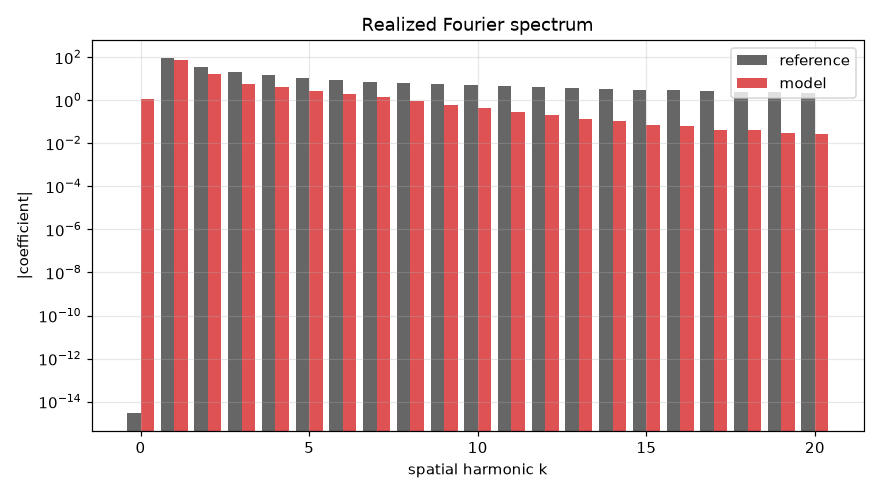
\includegraphics[width=\textwidth]{burgers_classical/figures/spectrum.png}
\caption{\textbf{burgers\_classical} --- Realized spatial spectrum (per-harmonic magnitude) vs.\ reference. Tests whether the model captures the high-$k$ shock tail or only low frequencies.}
\end{figure}
\begin{figure}[H]\centering
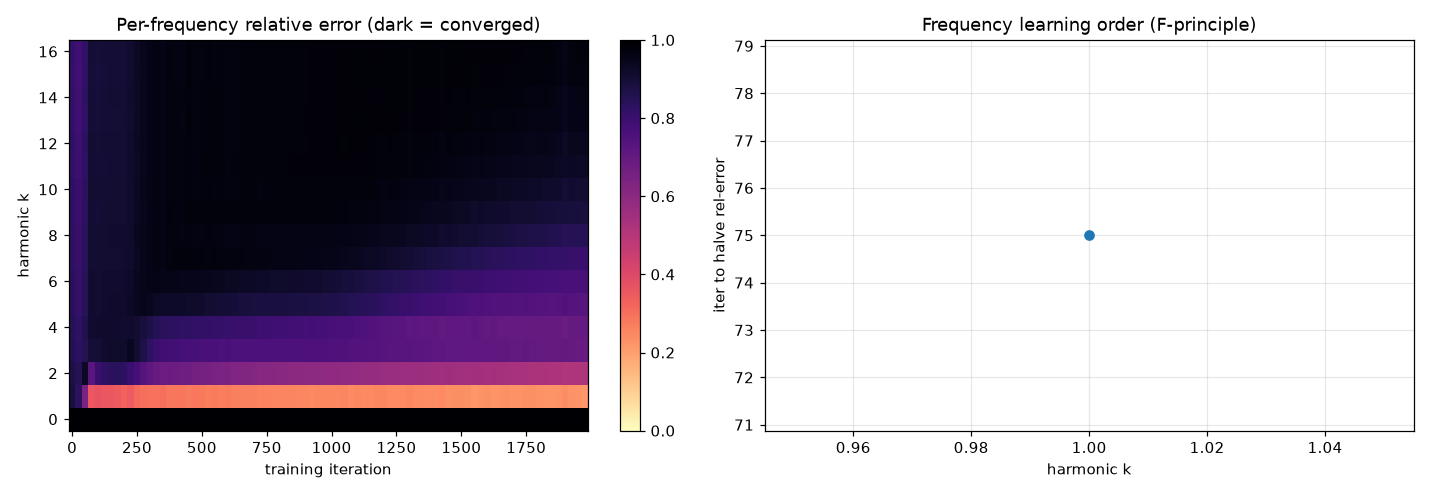
\includegraphics[width=\textwidth]{burgers_classical/figures/fprinciple.png}
\caption{\textbf{burgers\_classical} --- F-principle heat-map: iteration at which each harmonic's relative error halves. Low harmonics converging first is the F-principle signature.}
\end{figure}
\begin{figure}[H]\centering
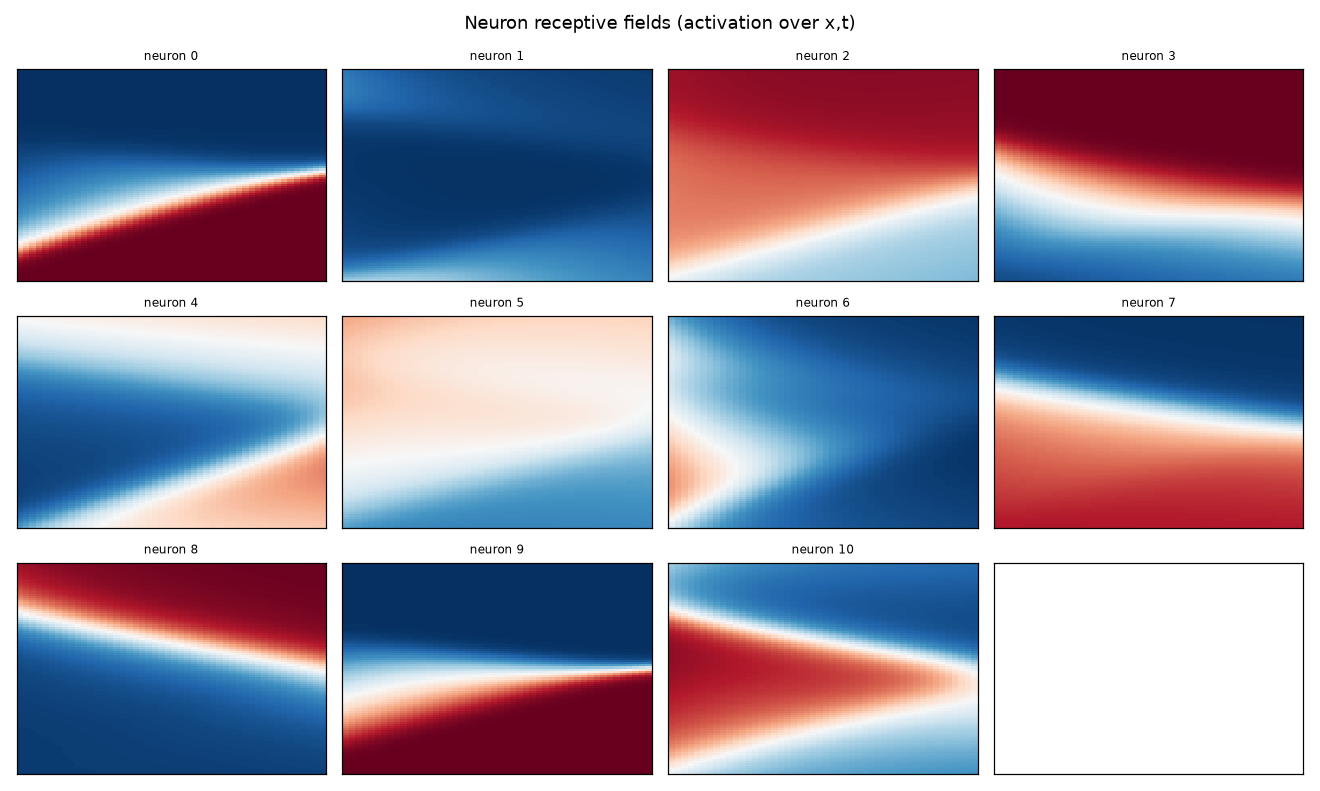
\includegraphics[width=\textwidth]{burgers_classical/figures/neurons.png}
\caption{\textbf{burgers\_classical} --- Classical post-net neurons: receptive fields over $(x,t)$ and each neuron's dominant spatial frequency / effective rank.}
\end{figure}
\begin{figure}[H]\centering
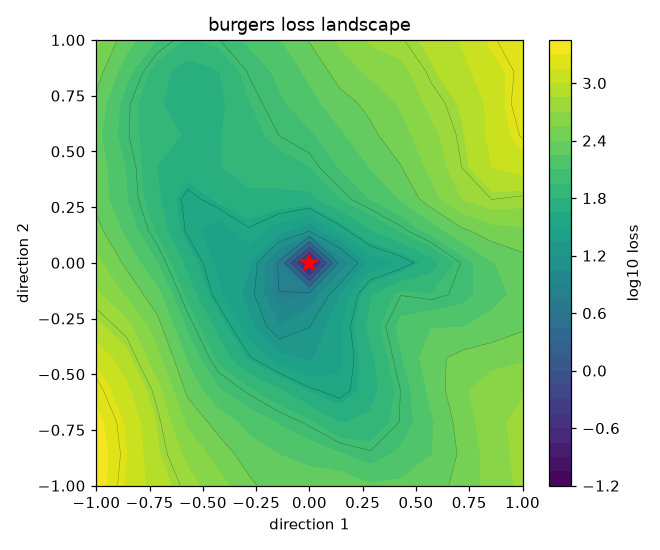
\includegraphics[width=\textwidth]{burgers_classical/figures/landscape.png}
\caption{\textbf{burgers\_classical} --- Filter-normalized 2-D loss landscape around the trained minimum (Li et al.\ 2018). Flat/wide vs.\ sharp basin.}
\end{figure}
\begin{figure}[H]\centering
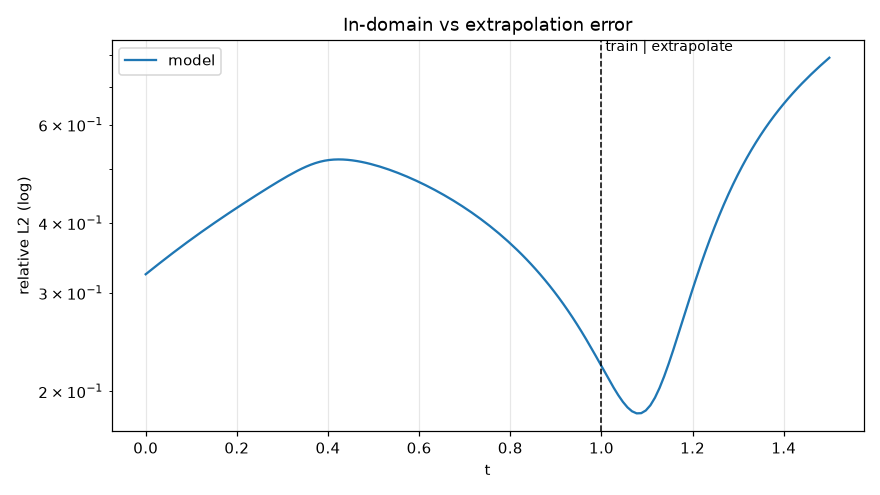
\includegraphics[width=\textwidth]{burgers_classical/figures/generalization.png}
\caption{\textbf{burgers\_classical} --- Extrapolation: relative $L_2$ vs.\ $t$ beyond the $t\in[0,1]$ training window --- the off-domain penalty.}
\end{figure}
\begin{figure}[H]\centering
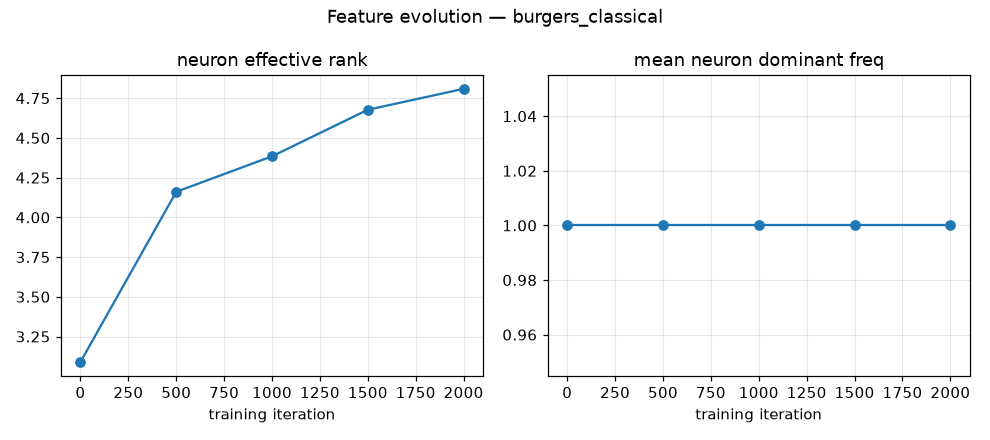
\includegraphics[width=\textwidth]{burgers_classical/figures/evolution.png}
\caption{\textbf{burgers\_classical} --- Solution evolution: snapshots of $u(x,\cdot)$ across time.}
\end{figure}
\begin{figure}[H]\centering
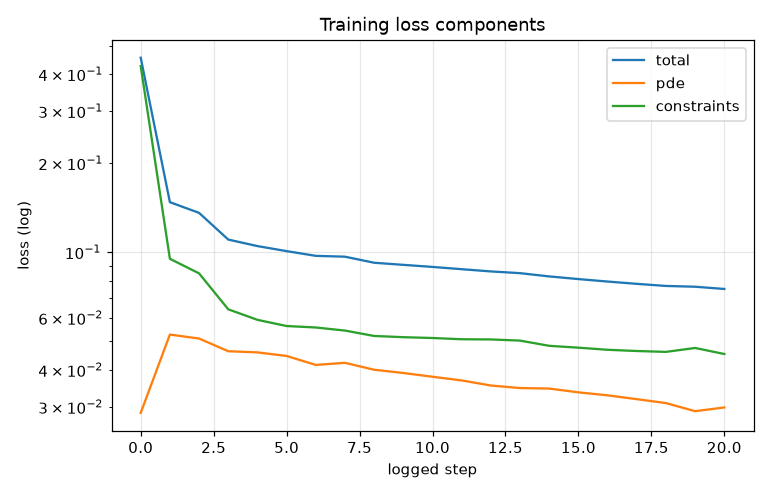
\includegraphics[width=\textwidth]{burgers_classical/figures/loss.png}
\caption{\textbf{burgers\_classical} --- Training loss history (total, PDE-residual, and constraint terms).}
\end{figure}
\clearpage
\subsection{burgers\_qapinn}
\noindent\small \textbf{rel-$L_2$}: 0.4722  \textbf{params}: 121  \textbf{PDE}: burgers  \textbf{Adam iters}: 2000  \textbf{seed}: 0  \textbf{model}: qapinn  \textbf{final PDE loss}: 3.85e-02  \textbf{wall time (s)}: 2010  \textbf{VQC}: 4q x3L ent=linear meas=multi scale=1.0\normalsize

\noindent\textbf{Observation.} Behaves almost identically to the classical Burgers run: shock at x=0 is smeared into a rounded sawtooth with amplitude capped at \textasciitilde{}0.65 (colorbar \textasciitilde{}0.66), and |error| shows the same bright bowtie about x=0 peaking \textasciitilde{}0.9. Spectrum agrees at k=1-2 then drops below the reference from k\textasciitilde{}3, reaching about 1.5 decades low at k=20 (model \textasciitilde{}0.04 vs \textasciitilde{}1). Entanglement S ranges \textasciitilde{}0.45 (dark band near x=0-0.25) to \textasciitilde{}1.05 (bright bottom-left corner x\textless{}-0.5,t\textless{}0.2), and qubit 0 again carries a dominant horizontal band while qubits 1-3 show milder diagonal structure. Inference: quantum embedding does not overcome the shock/spectral-bias limitation, matching the classical PINN's failure mode almost exactly.

\begin{figure}[H]\centering
\includegraphics[width=\textwidth]{burgers_qapinn/figures/solution.png}
\caption{\textbf{burgers\_qapinn} --- Predicted field $u(x,t)$ vs.\ exact reference, with the pointwise error map. The shock ($x\!=\!0$) is where a smooth network struggles.}
\end{figure}
\begin{figure}[H]\centering
\includegraphics[width=\textwidth]{burgers_qapinn/figures/spectrum.png}
\caption{\textbf{burgers\_qapinn} --- Realized spatial spectrum (per-harmonic magnitude) vs.\ reference. Tests whether the model captures the high-$k$ shock tail or only low frequencies.}
\end{figure}
\begin{figure}[H]\centering
\includegraphics[width=\textwidth]{burgers_qapinn/figures/fprinciple.png}
\caption{\textbf{burgers\_qapinn} --- F-principle heat-map: iteration at which each harmonic's relative error halves. Low harmonics converging first is the F-principle signature.}
\end{figure}
\begin{figure}[H]\centering
\includegraphics[width=\textwidth]{burgers_qapinn/figures/neurons.png}
\caption{\textbf{burgers\_qapinn} --- Classical post-net neurons: receptive fields over $(x,t)$ and each neuron's dominant spatial frequency / effective rank.}
\end{figure}
\begin{figure}[H]\centering
\includegraphics[width=\textwidth]{burgers_qapinn/figures/qubits.png}
\caption{\textbf{burgers\_qapinn} --- Per-qubit $\langle Z\rangle$ receptive fields --- what feature each qubit computes over the domain (quantum models only).}
\end{figure}
\begin{figure}[H]\centering
\includegraphics[width=\textwidth]{burgers_qapinn/figures/entanglement.png}
\caption{\textbf{burgers\_qapinn} --- Von Neumann entanglement entropy $S(x,t)$ of a qubit bipartition across the domain (quantum models only).}
\end{figure}
\begin{figure}[H]\centering
\includegraphics[width=\textwidth]{burgers_qapinn/figures/landscape.png}
\caption{\textbf{burgers\_qapinn} --- Filter-normalized 2-D loss landscape around the trained minimum (Li et al.\ 2018). Flat/wide vs.\ sharp basin.}
\end{figure}
\begin{figure}[H]\centering
\includegraphics[width=\textwidth]{burgers_qapinn/figures/generalization.png}
\caption{\textbf{burgers\_qapinn} --- Extrapolation: relative $L_2$ vs.\ $t$ beyond the $t\in[0,1]$ training window --- the off-domain penalty.}
\end{figure}
\begin{figure}[H]\centering
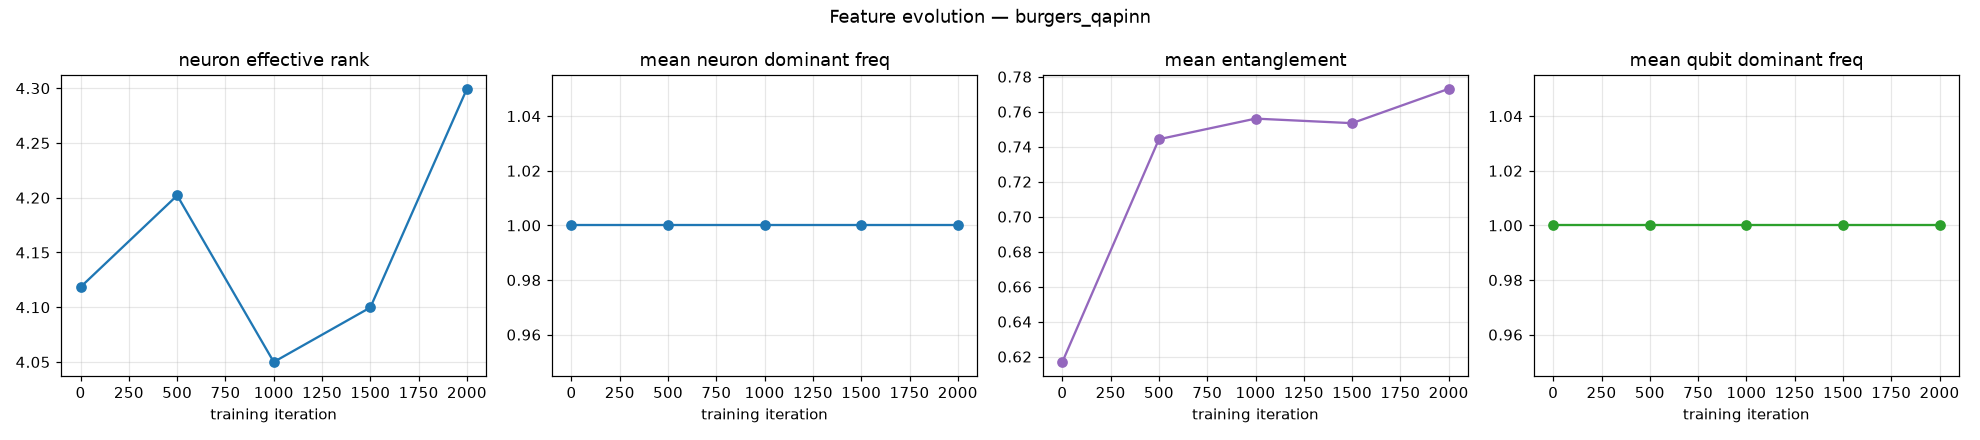
\includegraphics[width=\textwidth]{burgers_qapinn/figures/evolution.png}
\caption{\textbf{burgers\_qapinn} --- Solution evolution: snapshots of $u(x,\cdot)$ across time.}
\end{figure}
\begin{figure}[H]\centering
\includegraphics[width=\textwidth]{burgers_qapinn/figures/loss.png}
\caption{\textbf{burgers\_qapinn} --- Training loss history (total, PDE-residual, and constraint terms).}
\end{figure}
\clearpage
\section{Tier-1 ablation --- re-upload depth (the bandwidth axis)}
Depth sets the VQC's accessible Fourier band $\{-L..L\}$. Prediction: accuracy and realized bandwidth grow with depth. The depth-3 point is the reference run.

\subsection{abl\_depth\_1}
\noindent\small \textbf{rel-$L_2$}: 0.5717  \textbf{params}: 105  \textbf{PDE}: burgers  \textbf{Adam iters}: 2000  \textbf{seed}: 0  \textbf{model}: qapinn  \textbf{final PDE loss}: 5.76e-02  \textbf{wall time (s)}: 624  \textbf{VQC}: 4q x1L ent=linear meas=multi scale=1.0\normalsize

\noindent\textbf{Observation.} Shallowest circuit and the weakest fit: prediction amplitude is capped hardest at \textasciitilde{}0.6 (colorbar \textasciitilde{}0.6) and the sawtooth is the most rounded of the set, with the |error| bowtie about x=0 still reaching \textasciitilde{}0.9. Spectrum tracks k=1-2 then drops below reference from k\textasciitilde{}2-3 with the model bars flattening to \textasciitilde{}0.06-0.08 by k=20. Most notably the entanglement collapses to a low range S \textasciitilde{}0.05-0.55 (far below baseline's \textasciitilde{}1.05), concentrated only in the upper-right corner (x\textgreater{}0.5, t\textgreater{}0.8); the \textless{}Z\textgreater{} maps are simple monotone gradients with little structure. Inference: too few layers starves the model of entanglement/expressivity, giving the lowest amplitude and flattest high-k response.

\begin{figure}[H]\centering
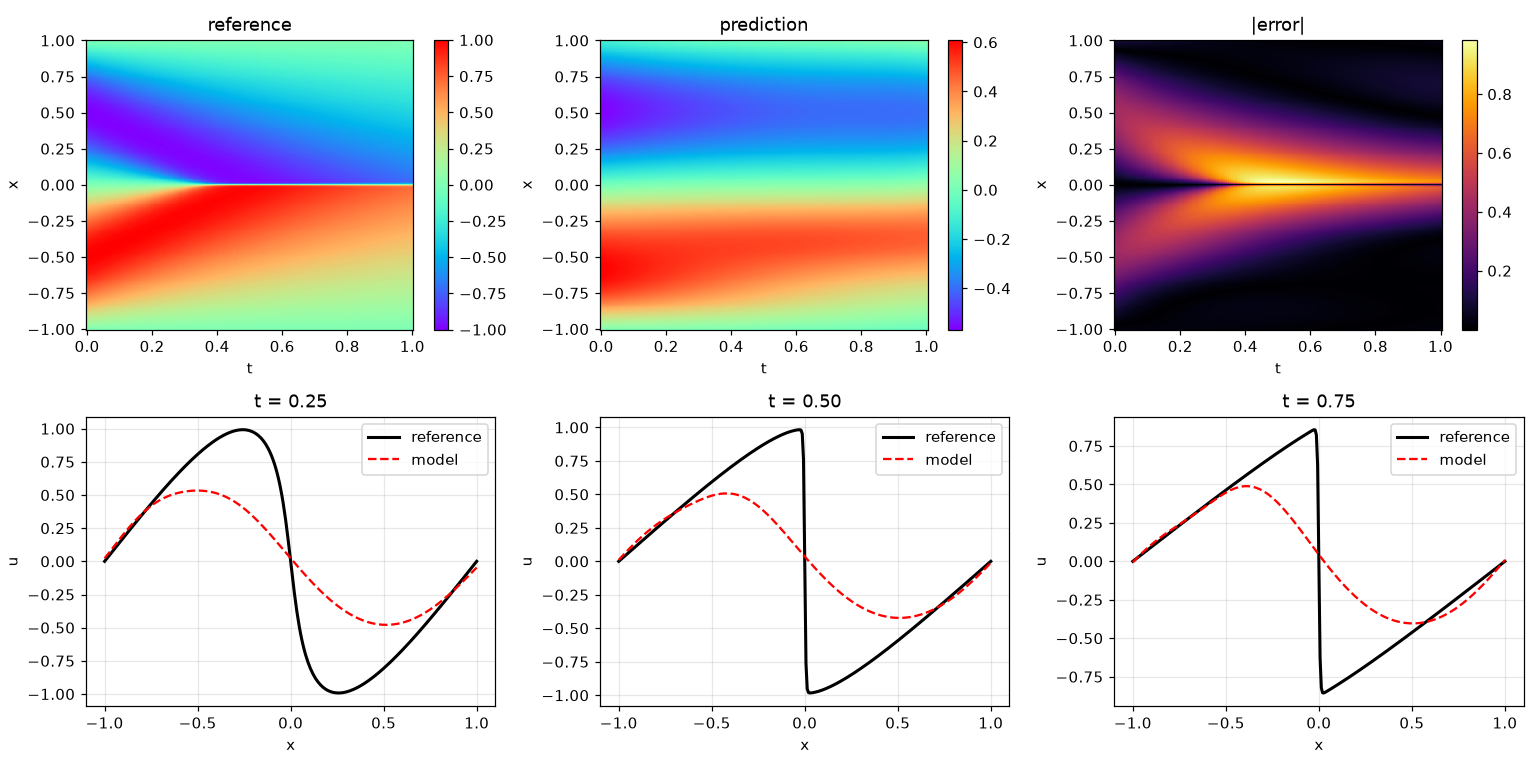
\includegraphics[width=\textwidth]{abl_depth_1/figures/solution.png}
\caption{\textbf{abl\_depth\_1} --- Predicted field $u(x,t)$ vs.\ exact reference, with the pointwise error map. The shock ($x\!=\!0$) is where a smooth network struggles.}
\end{figure}
\begin{figure}[H]\centering
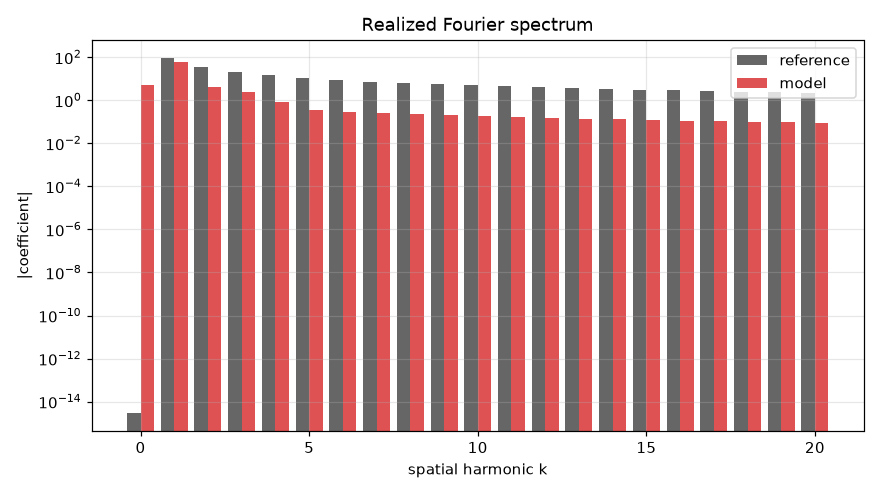
\includegraphics[width=\textwidth]{abl_depth_1/figures/spectrum.png}
\caption{\textbf{abl\_depth\_1} --- Realized spatial spectrum (per-harmonic magnitude) vs.\ reference. Tests whether the model captures the high-$k$ shock tail or only low frequencies.}
\end{figure}
\begin{figure}[H]\centering
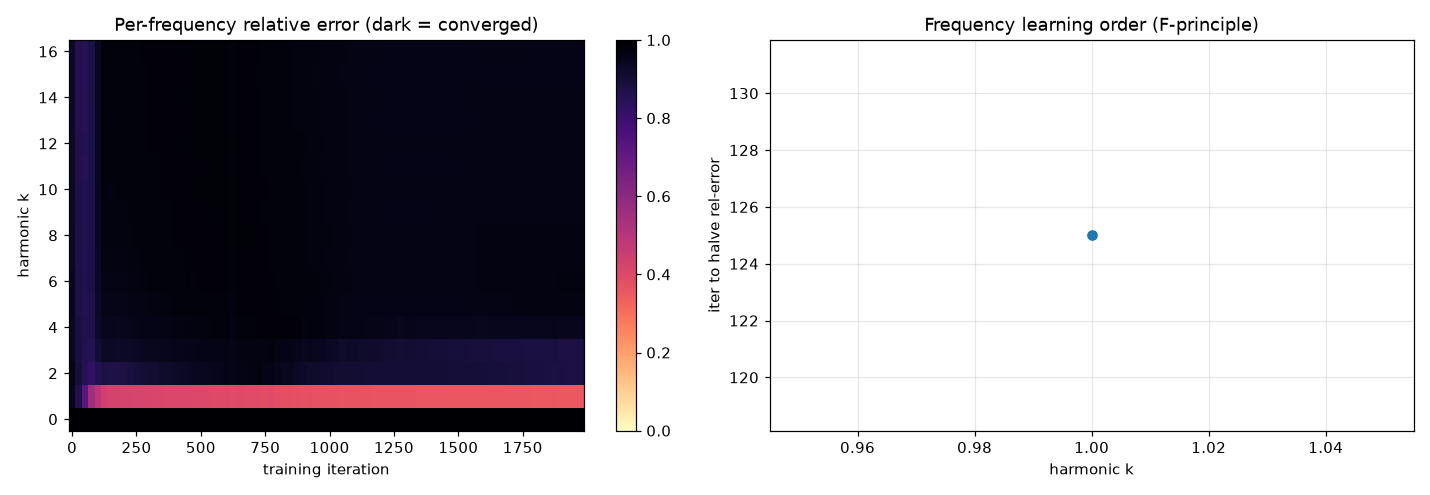
\includegraphics[width=\textwidth]{abl_depth_1/figures/fprinciple.png}
\caption{\textbf{abl\_depth\_1} --- F-principle heat-map: iteration at which each harmonic's relative error halves. Low harmonics converging first is the F-principle signature.}
\end{figure}
\begin{figure}[H]\centering
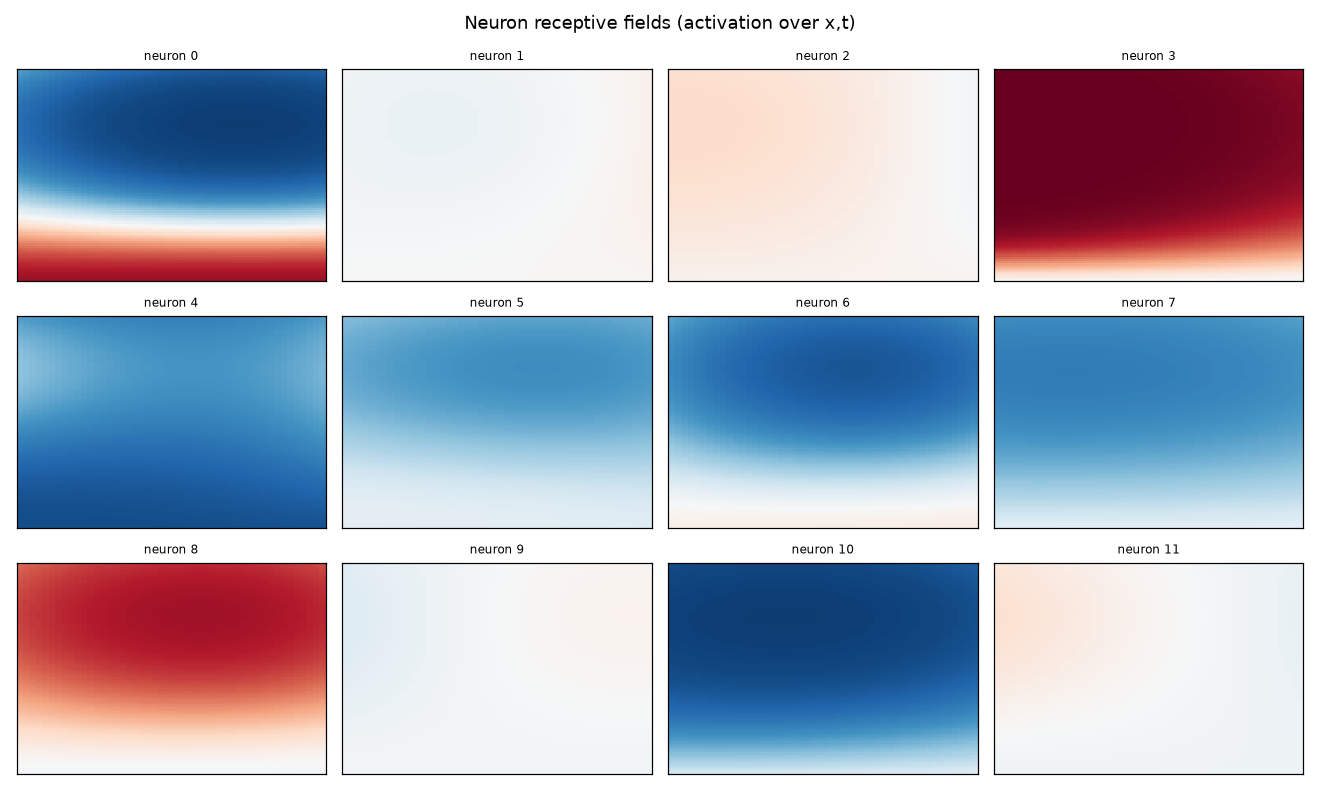
\includegraphics[width=\textwidth]{abl_depth_1/figures/neurons.png}
\caption{\textbf{abl\_depth\_1} --- Classical post-net neurons: receptive fields over $(x,t)$ and each neuron's dominant spatial frequency / effective rank.}
\end{figure}
\begin{figure}[H]\centering
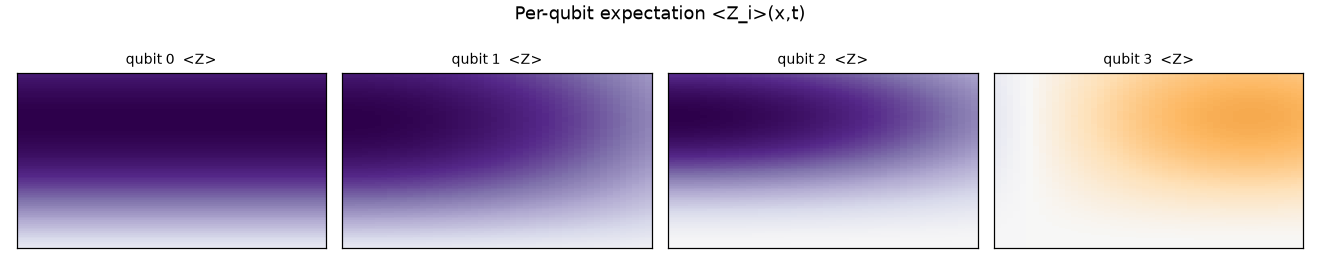
\includegraphics[width=\textwidth]{abl_depth_1/figures/qubits.png}
\caption{\textbf{abl\_depth\_1} --- Per-qubit $\langle Z\rangle$ receptive fields --- what feature each qubit computes over the domain (quantum models only).}
\end{figure}
\begin{figure}[H]\centering
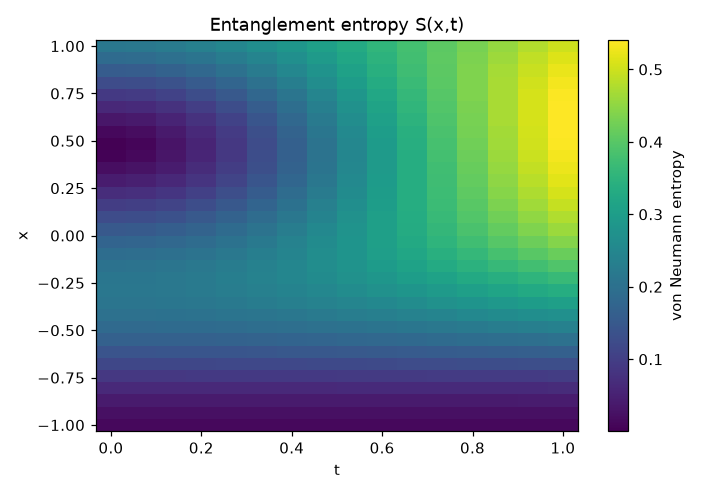
\includegraphics[width=\textwidth]{abl_depth_1/figures/entanglement.png}
\caption{\textbf{abl\_depth\_1} --- Von Neumann entanglement entropy $S(x,t)$ of a qubit bipartition across the domain (quantum models only).}
\end{figure}
\begin{figure}[H]\centering
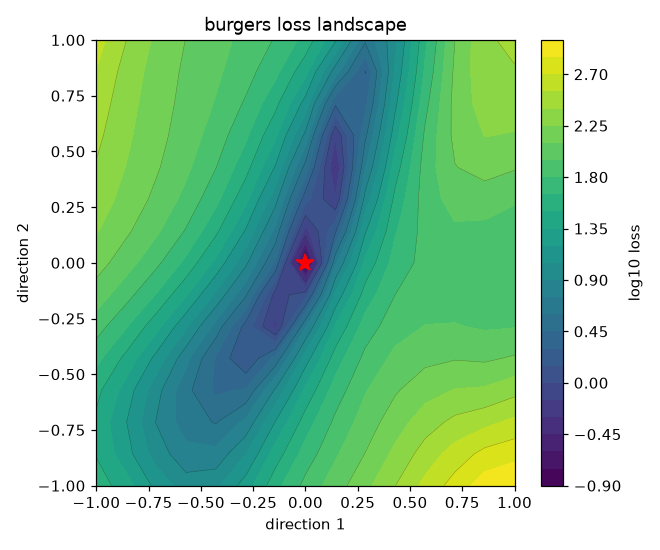
\includegraphics[width=\textwidth]{abl_depth_1/figures/landscape.png}
\caption{\textbf{abl\_depth\_1} --- Filter-normalized 2-D loss landscape around the trained minimum (Li et al.\ 2018). Flat/wide vs.\ sharp basin.}
\end{figure}
\begin{figure}[H]\centering
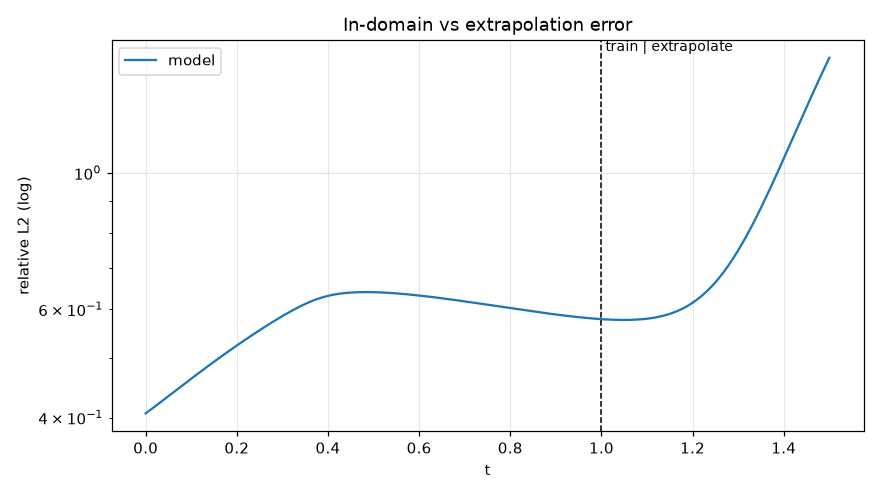
\includegraphics[width=\textwidth]{abl_depth_1/figures/generalization.png}
\caption{\textbf{abl\_depth\_1} --- Extrapolation: relative $L_2$ vs.\ $t$ beyond the $t\in[0,1]$ training window --- the off-domain penalty.}
\end{figure}
\begin{figure}[H]\centering
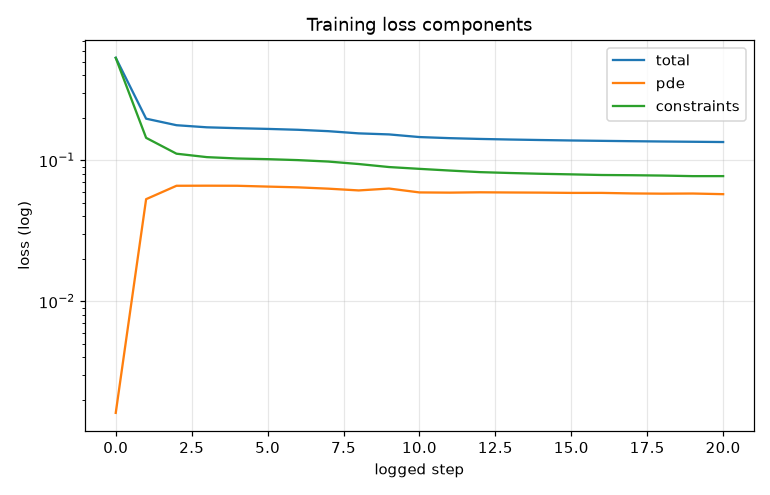
\includegraphics[width=\textwidth]{abl_depth_1/figures/loss.png}
\caption{\textbf{abl\_depth\_1} --- Training loss history (total, PDE-residual, and constraint terms).}
\end{figure}
\clearpage
\subsection{abl\_depth\_2}
\noindent\small \textbf{rel-$L_2$}: 0.4930  \textbf{params}: 113  \textbf{PDE}: burgers  \textbf{Adam iters}: 2000  \textbf{seed}: 0  \textbf{model}: qapinn  \textbf{final PDE loss}: 4.60e-02  \textbf{wall time (s)}: 1157  \textbf{VQC}: 4q x2L ent=linear meas=multi scale=1.0\normalsize

\noindent\textbf{Observation.} Intermediate depth: prediction still amplitude-capped \textasciitilde{}0.6 with the same smeared shock and \textasciitilde{}0.9 |error| bowtie about x=0, so solution quality is barely changed from depth 1. Spectrum matches k=1-2 then falls below reference from k\textasciitilde{}3, similar to baseline. Entanglement recovers to a mid range S \textasciitilde{}0.35-0.98 (bright peak in the top-right corner, dark patch bottom-right), sitting between depth\_1 (\textasciitilde{}0.55 max) and baseline (\textasciitilde{}1.05 max); qubits 0-1 show antisymmetric horizontal bands while qubits 2-3 are fainter. Inference: added depth mainly raises entanglement capacity but yields only marginal gains in the realized shock solution.

\begin{figure}[H]\centering
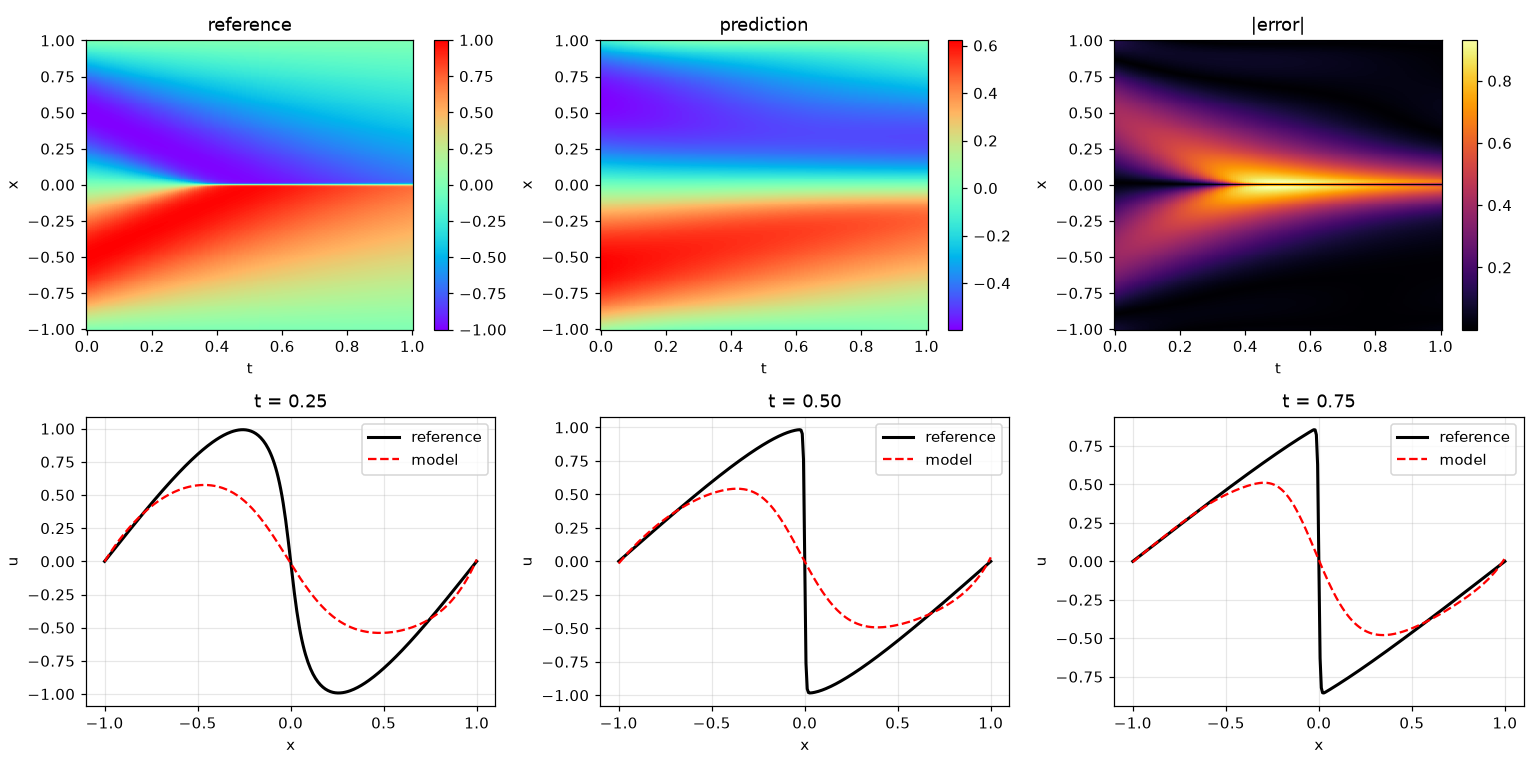
\includegraphics[width=\textwidth]{abl_depth_2/figures/solution.png}
\caption{\textbf{abl\_depth\_2} --- Predicted field $u(x,t)$ vs.\ exact reference, with the pointwise error map. The shock ($x\!=\!0$) is where a smooth network struggles.}
\end{figure}
\begin{figure}[H]\centering
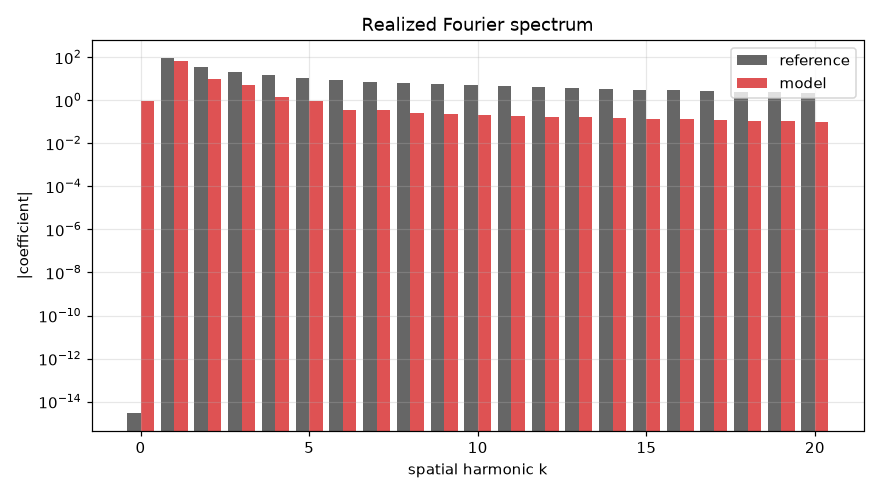
\includegraphics[width=\textwidth]{abl_depth_2/figures/spectrum.png}
\caption{\textbf{abl\_depth\_2} --- Realized spatial spectrum (per-harmonic magnitude) vs.\ reference. Tests whether the model captures the high-$k$ shock tail or only low frequencies.}
\end{figure}
\begin{figure}[H]\centering
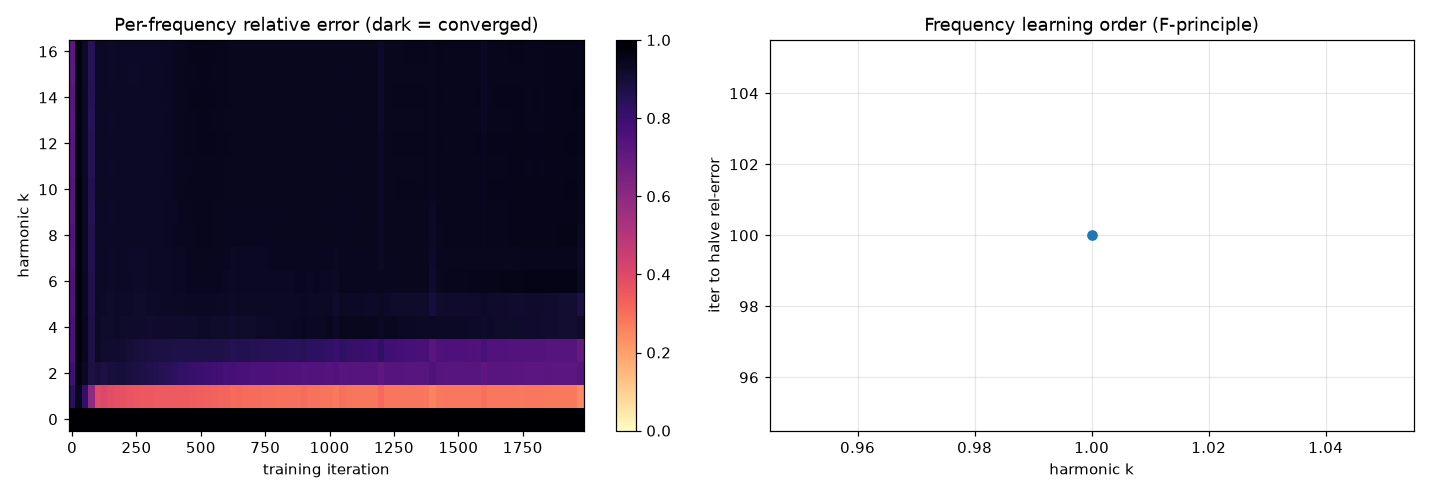
\includegraphics[width=\textwidth]{abl_depth_2/figures/fprinciple.png}
\caption{\textbf{abl\_depth\_2} --- F-principle heat-map: iteration at which each harmonic's relative error halves. Low harmonics converging first is the F-principle signature.}
\end{figure}
\begin{figure}[H]\centering
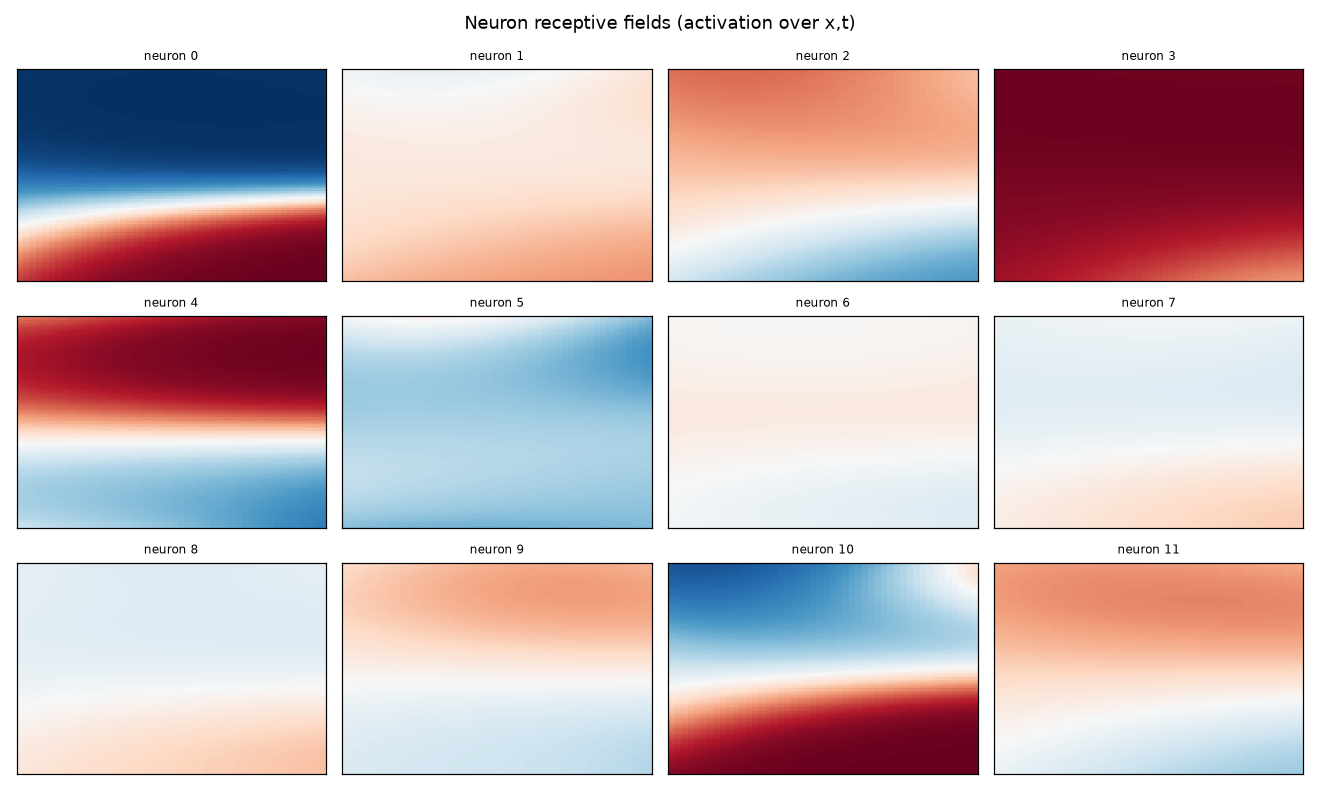
\includegraphics[width=\textwidth]{abl_depth_2/figures/neurons.png}
\caption{\textbf{abl\_depth\_2} --- Classical post-net neurons: receptive fields over $(x,t)$ and each neuron's dominant spatial frequency / effective rank.}
\end{figure}
\begin{figure}[H]\centering
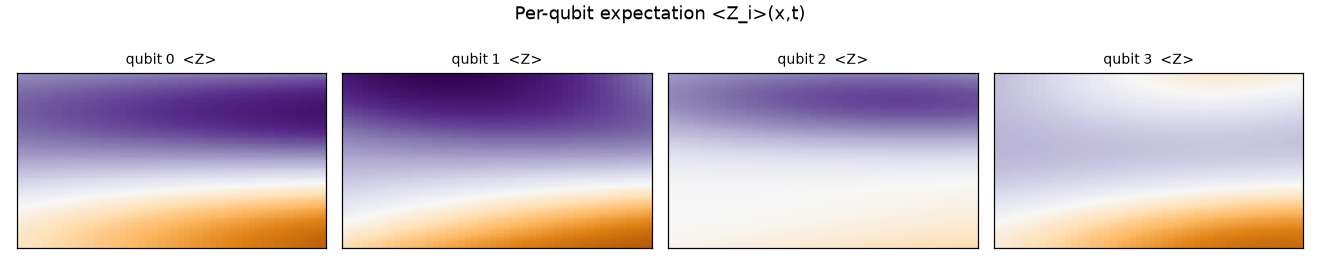
\includegraphics[width=\textwidth]{abl_depth_2/figures/qubits.png}
\caption{\textbf{abl\_depth\_2} --- Per-qubit $\langle Z\rangle$ receptive fields --- what feature each qubit computes over the domain (quantum models only).}
\end{figure}
\begin{figure}[H]\centering
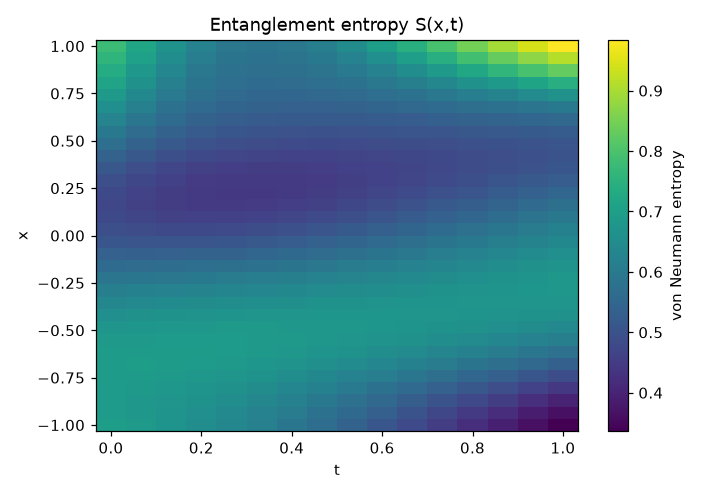
\includegraphics[width=\textwidth]{abl_depth_2/figures/entanglement.png}
\caption{\textbf{abl\_depth\_2} --- Von Neumann entanglement entropy $S(x,t)$ of a qubit bipartition across the domain (quantum models only).}
\end{figure}
\begin{figure}[H]\centering
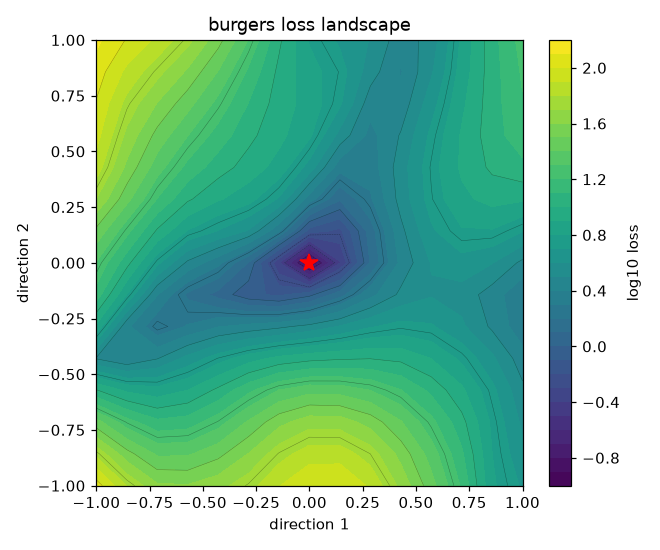
\includegraphics[width=\textwidth]{abl_depth_2/figures/landscape.png}
\caption{\textbf{abl\_depth\_2} --- Filter-normalized 2-D loss landscape around the trained minimum (Li et al.\ 2018). Flat/wide vs.\ sharp basin.}
\end{figure}
\begin{figure}[H]\centering
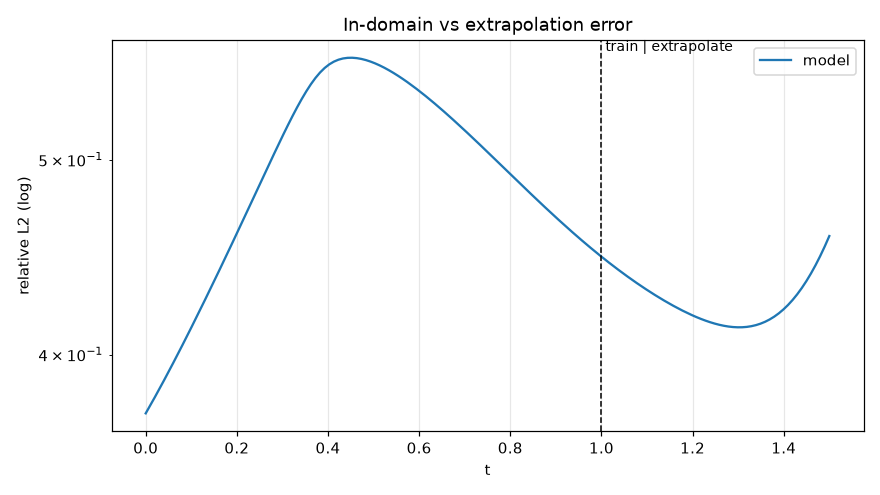
\includegraphics[width=\textwidth]{abl_depth_2/figures/generalization.png}
\caption{\textbf{abl\_depth\_2} --- Extrapolation: relative $L_2$ vs.\ $t$ beyond the $t\in[0,1]$ training window --- the off-domain penalty.}
\end{figure}
\begin{figure}[H]\centering
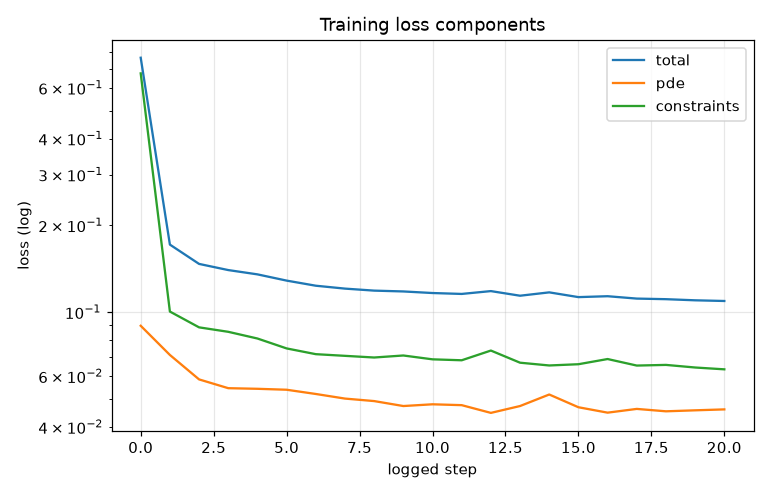
\includegraphics[width=\textwidth]{abl_depth_2/figures/loss.png}
\caption{\textbf{abl\_depth\_2} --- Training loss history (total, PDE-residual, and constraint terms).}
\end{figure}
\clearpage
\subsection{abl\_depth\_5}
\noindent\small \textbf{rel-$L_2$}: 0.4241  \textbf{params}: 137  \textbf{PDE}: burgers  \textbf{Adam iters}: 2000  \textbf{seed}: 0  \textbf{model}: qapinn  \textbf{final PDE loss}: 3.44e-02  \textbf{wall time (s)}: 2778  \textbf{VQC}: 4q x5L ent=linear meas=multi scale=1.0\normalsize

\noindent\textbf{Observation.} Deepest circuit and marginally the best of the Burgers/ablation set: prediction amplitude recovers to \textasciitilde{}0.65 and the sawtooth is slightly sharper, though the shock is still smoothed and the |error| bowtie about x=0 remains \textasciitilde{}0.9. Spectrum holds a hair closer to the reference through mid-k but still falls off from k\textasciitilde{}3, ending \textasciitilde{}0.05 at k=20. Entanglement is the highest and most structured, S \textasciitilde{}0.6-1.2, with a distinct bright blob at x\textasciitilde{}0,t\textasciitilde{}0.3 (\textasciitilde{}1.2) and a dark trough near x=-0.5,t\textasciitilde{}0.7 (\textasciitilde{}0.6); the \textless{}Z\textgreater{} qubit maps are visibly more oscillatory with sign changes across qubits. Inference: more layers monotonically increase entanglement (0.55 -\textgreater{} 0.98 -\textgreater{} 1.05 -\textgreater{} 1.2 across depths 1/2/baseline/5) and richer qubit features, but only modestly improve the shock fit, confirming depth helps expressivity more than it cures spectral bias.

\begin{figure}[H]\centering
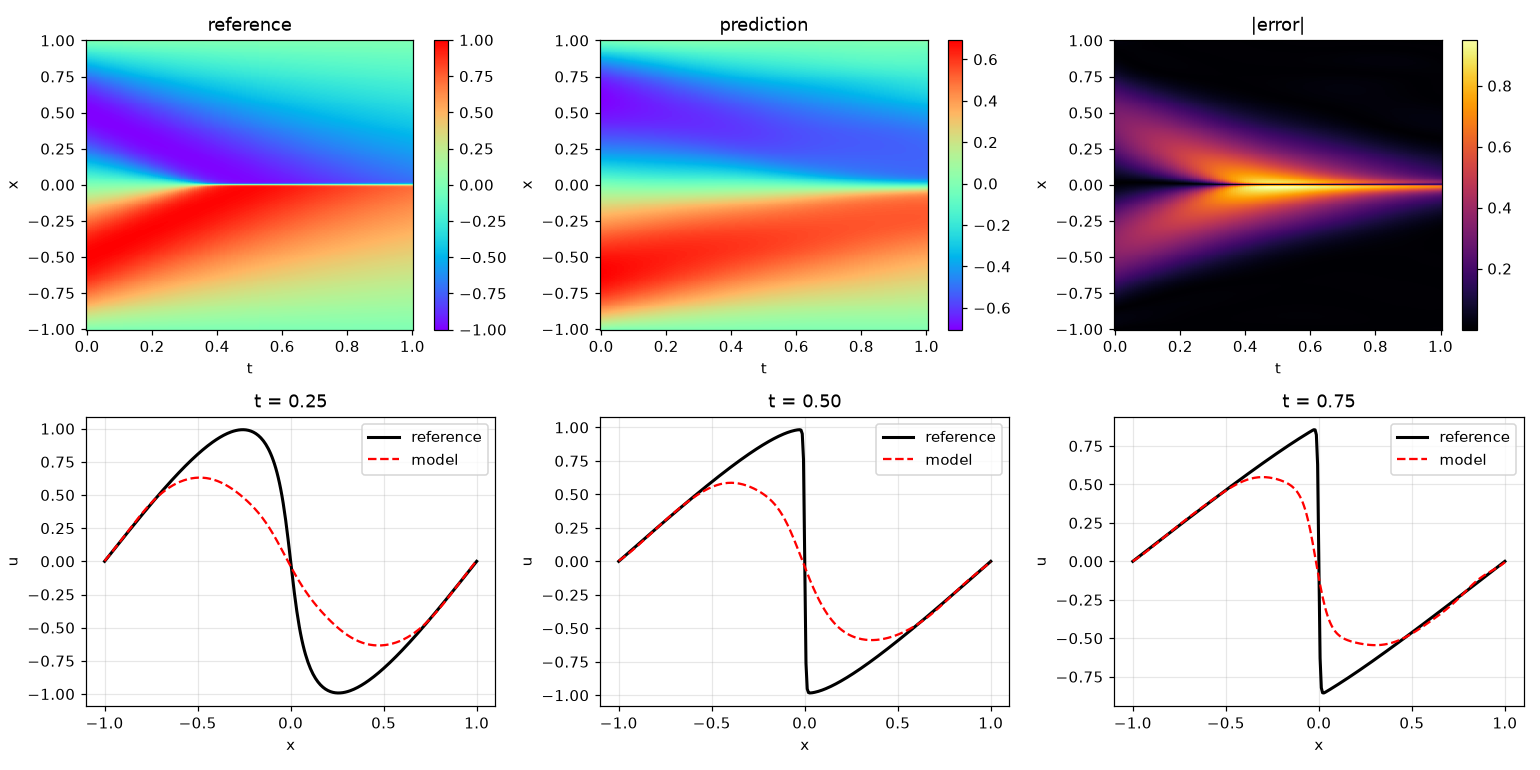
\includegraphics[width=\textwidth]{abl_depth_5/figures/solution.png}
\caption{\textbf{abl\_depth\_5} --- Predicted field $u(x,t)$ vs.\ exact reference, with the pointwise error map. The shock ($x\!=\!0$) is where a smooth network struggles.}
\end{figure}
\begin{figure}[H]\centering
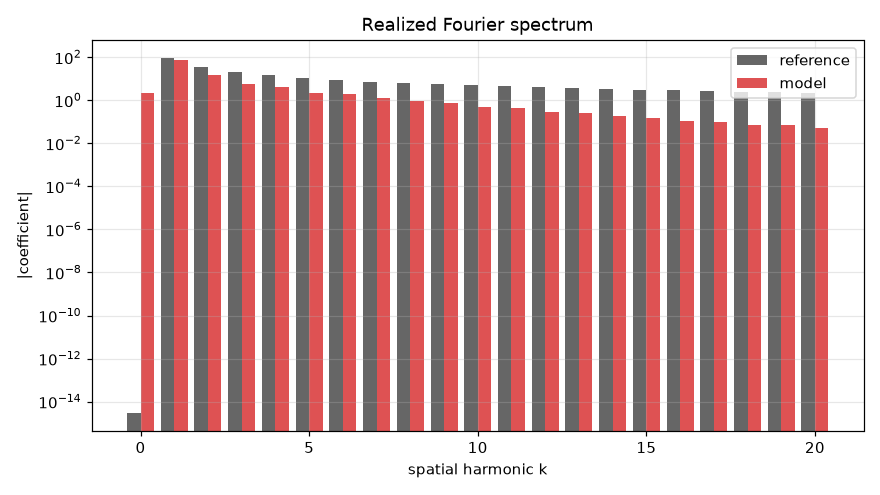
\includegraphics[width=\textwidth]{abl_depth_5/figures/spectrum.png}
\caption{\textbf{abl\_depth\_5} --- Realized spatial spectrum (per-harmonic magnitude) vs.\ reference. Tests whether the model captures the high-$k$ shock tail or only low frequencies.}
\end{figure}
\begin{figure}[H]\centering
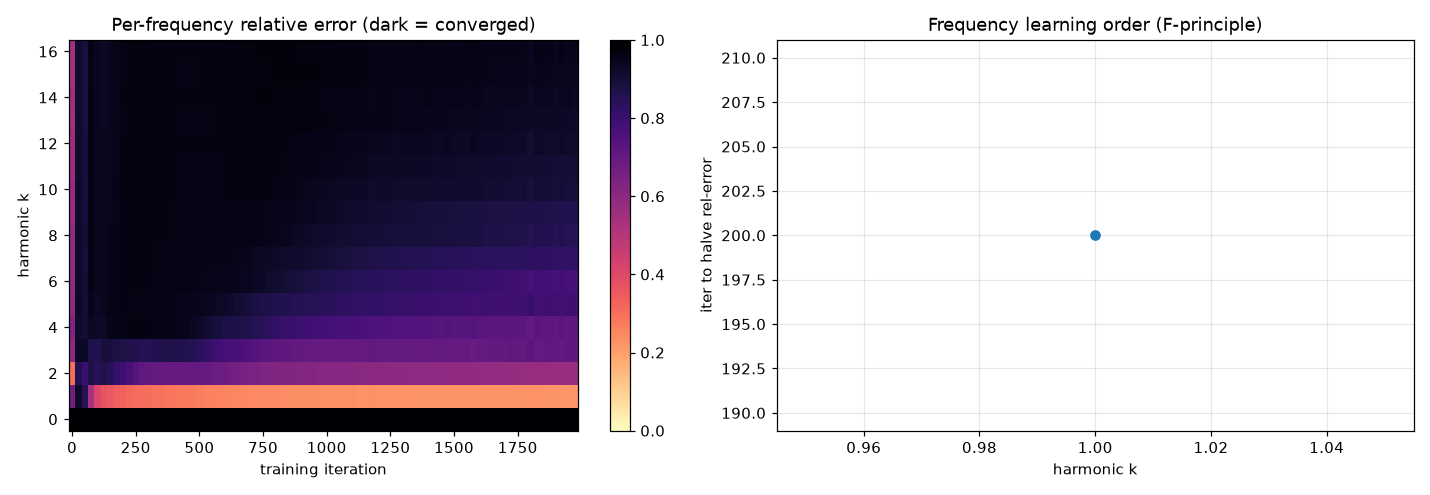
\includegraphics[width=\textwidth]{abl_depth_5/figures/fprinciple.png}
\caption{\textbf{abl\_depth\_5} --- F-principle heat-map: iteration at which each harmonic's relative error halves. Low harmonics converging first is the F-principle signature.}
\end{figure}
\begin{figure}[H]\centering
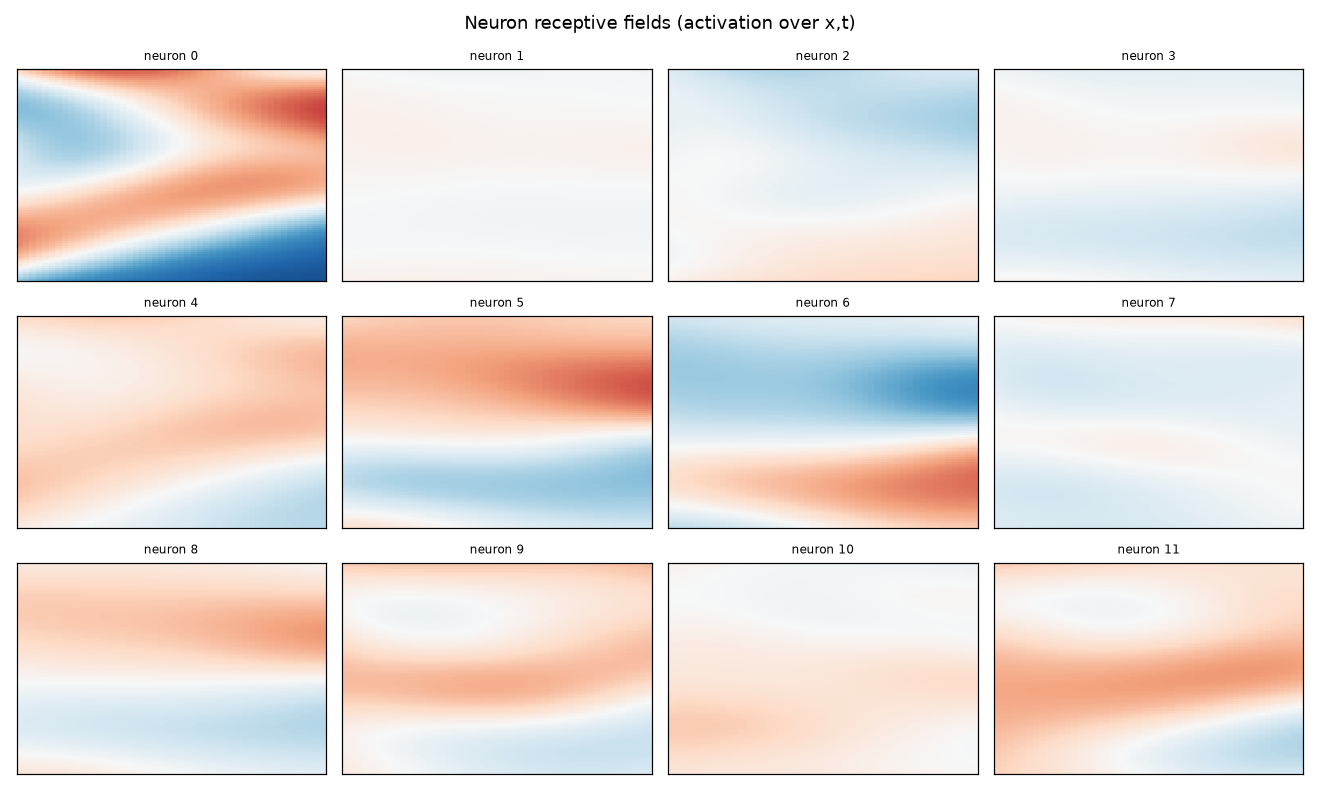
\includegraphics[width=\textwidth]{abl_depth_5/figures/neurons.png}
\caption{\textbf{abl\_depth\_5} --- Classical post-net neurons: receptive fields over $(x,t)$ and each neuron's dominant spatial frequency / effective rank.}
\end{figure}
\begin{figure}[H]\centering
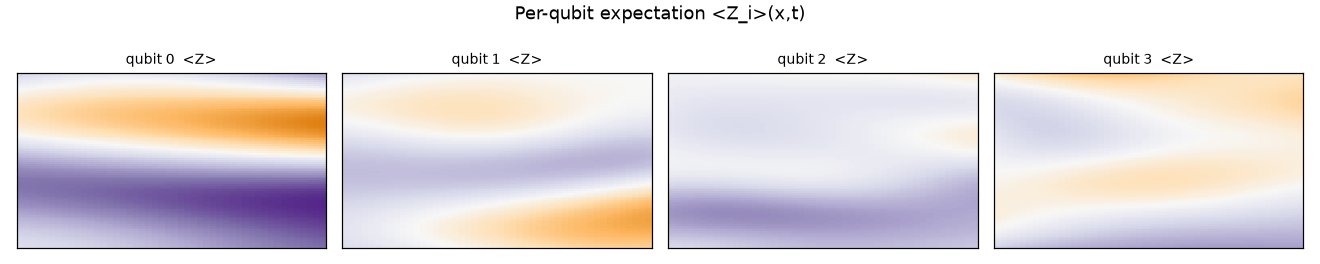
\includegraphics[width=\textwidth]{abl_depth_5/figures/qubits.png}
\caption{\textbf{abl\_depth\_5} --- Per-qubit $\langle Z\rangle$ receptive fields --- what feature each qubit computes over the domain (quantum models only).}
\end{figure}
\begin{figure}[H]\centering
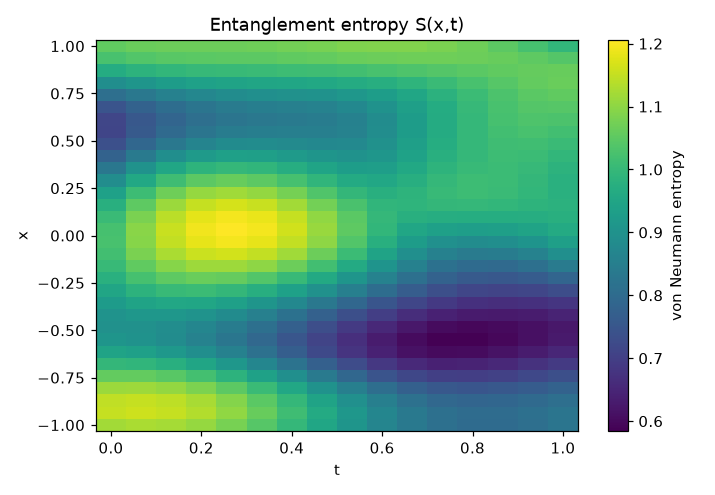
\includegraphics[width=\textwidth]{abl_depth_5/figures/entanglement.png}
\caption{\textbf{abl\_depth\_5} --- Von Neumann entanglement entropy $S(x,t)$ of a qubit bipartition across the domain (quantum models only).}
\end{figure}
\begin{figure}[H]\centering
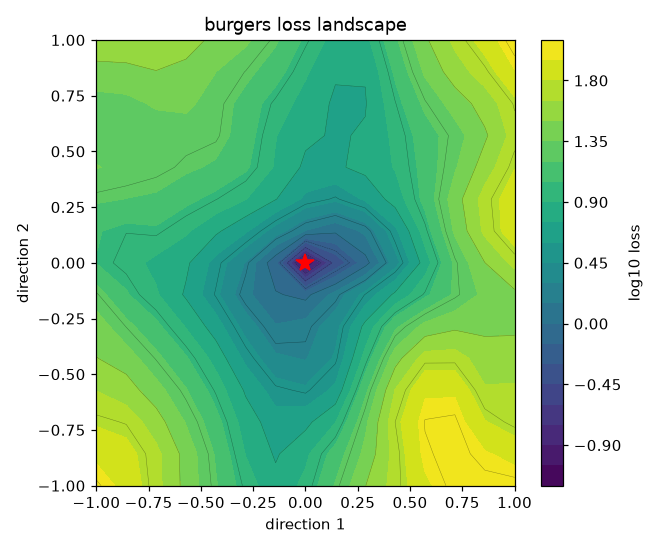
\includegraphics[width=\textwidth]{abl_depth_5/figures/landscape.png}
\caption{\textbf{abl\_depth\_5} --- Filter-normalized 2-D loss landscape around the trained minimum (Li et al.\ 2018). Flat/wide vs.\ sharp basin.}
\end{figure}
\begin{figure}[H]\centering
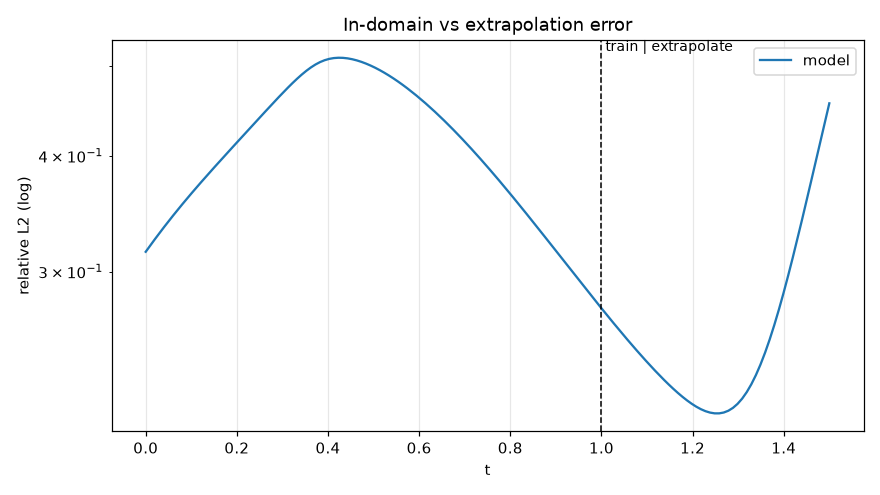
\includegraphics[width=\textwidth]{abl_depth_5/figures/generalization.png}
\caption{\textbf{abl\_depth\_5} --- Extrapolation: relative $L_2$ vs.\ $t$ beyond the $t\in[0,1]$ training window --- the off-domain penalty.}
\end{figure}
\begin{figure}[H]\centering
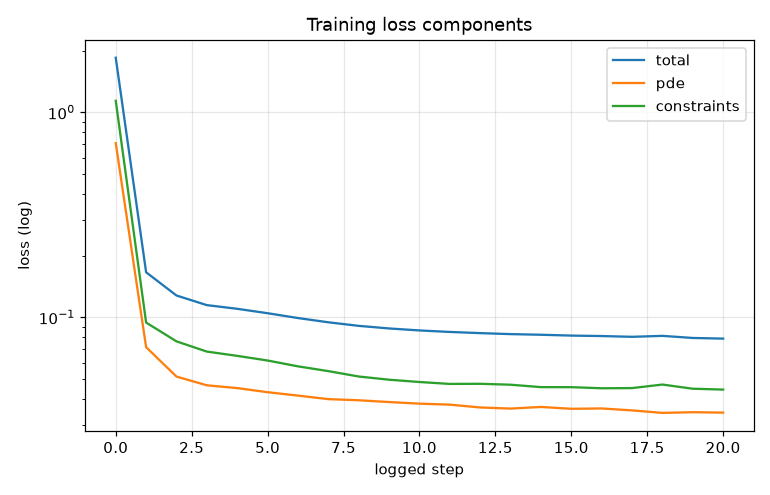
\includegraphics[width=\textwidth]{abl_depth_5/figures/loss.png}
\caption{\textbf{abl\_depth\_5} --- Training loss history (total, PDE-residual, and constraint terms).}
\end{figure}
\clearpage
\section{Tier-1 ablation --- entanglement structure (band fixed)}
Band held fixed; only the wiring changes (none/linear/ring/all-to-all). Tests whether entanglement (a coefficient/reachability knob) moves the advantage. Linear is the reference run.

\subsection{abl\_ent\_none}
\noindent\small \textbf{rel-$L_2$}: 0.4562  \textbf{params}: 121  \textbf{PDE}: burgers  \textbf{Adam iters}: 2000  \textbf{seed}: 0  \textbf{model}: qapinn  \textbf{final PDE loss}: 3.88e-02  \textbf{wall time (s)}: 1634  \textbf{VQC}: 4q x3L ent=none meas=multi scale=1.0\normalsize

\noindent\textbf{Observation.} Prediction amplitude caps at \textasciitilde{}+/-0.6 vs the reference +/-1.0, so the model reproduces the smooth sinusoidal ramps but rounds off both peaks; the |error| map (peaking \textasciitilde{}0.9) concentrates in a bright horizontal band at the x=0 shock, widening toward t\textasciitilde{}0.4-0.6, and the t=0.25/0.50/0.75 slices show the red model curve completely failing to capture the steepening jump at x=0. The realized Fourier spectrum tracks the reference for k=1-2 but the model bars fall progressively below reference from about k=4 onward and drop roughly an order of magnitude by k\textasciitilde{}11-12. Entanglement entropy is essentially zero (colorbar scale 1e-7, values within +/-6e-7, just numerical noise in a faint checkerboard), confirming the product-state/no-entangler wiring; per-qubit \textless{}Z\textgreater{} maps show clean, well-differentiated structure (qubits 0 and 2 horizontal x-banded, qubits 1 and 3 vertical t-gradients). Inference: with entanglement disabled the circuit still fits low harmonics via the classical net but cannot represent the shock, so this run behaves like a purely classical PINN with the QC layer contributing nothing.

\begin{figure}[H]\centering
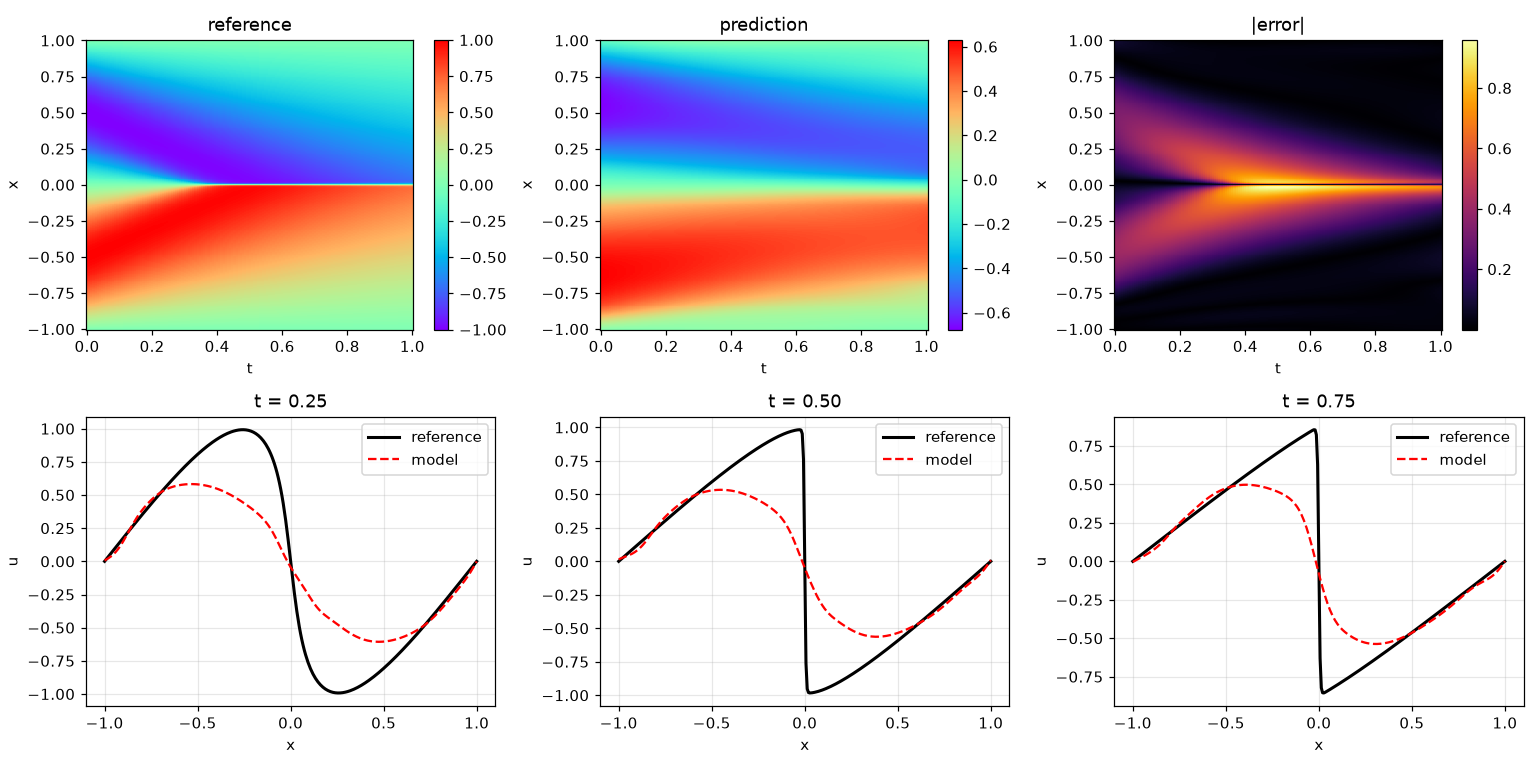
\includegraphics[width=\textwidth]{abl_ent_none/figures/solution.png}
\caption{\textbf{abl\_ent\_none} --- Predicted field $u(x,t)$ vs.\ exact reference, with the pointwise error map. The shock ($x\!=\!0$) is where a smooth network struggles.}
\end{figure}
\begin{figure}[H]\centering
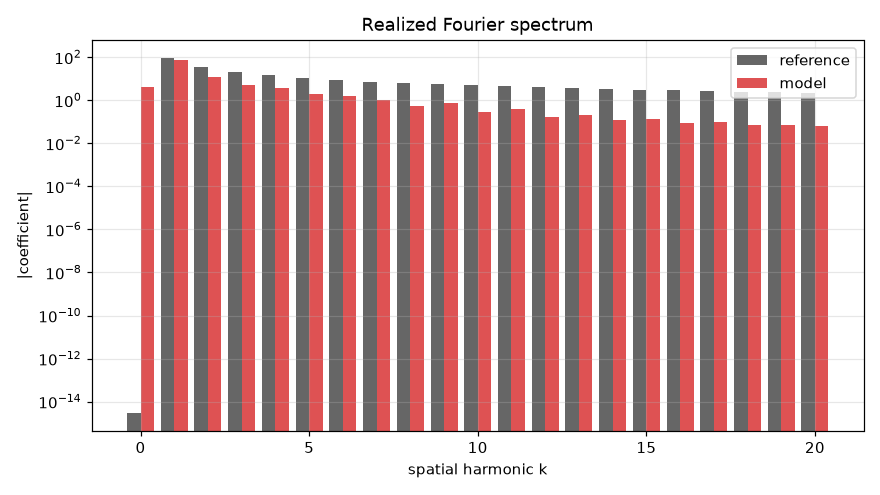
\includegraphics[width=\textwidth]{abl_ent_none/figures/spectrum.png}
\caption{\textbf{abl\_ent\_none} --- Realized spatial spectrum (per-harmonic magnitude) vs.\ reference. Tests whether the model captures the high-$k$ shock tail or only low frequencies.}
\end{figure}
\begin{figure}[H]\centering
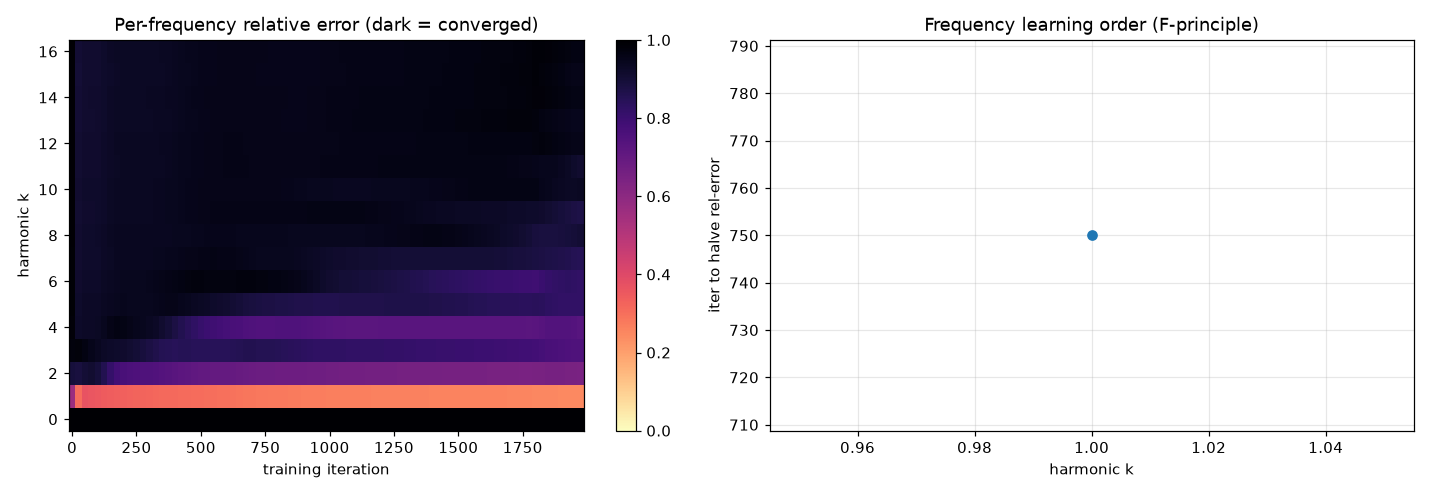
\includegraphics[width=\textwidth]{abl_ent_none/figures/fprinciple.png}
\caption{\textbf{abl\_ent\_none} --- F-principle heat-map: iteration at which each harmonic's relative error halves. Low harmonics converging first is the F-principle signature.}
\end{figure}
\begin{figure}[H]\centering
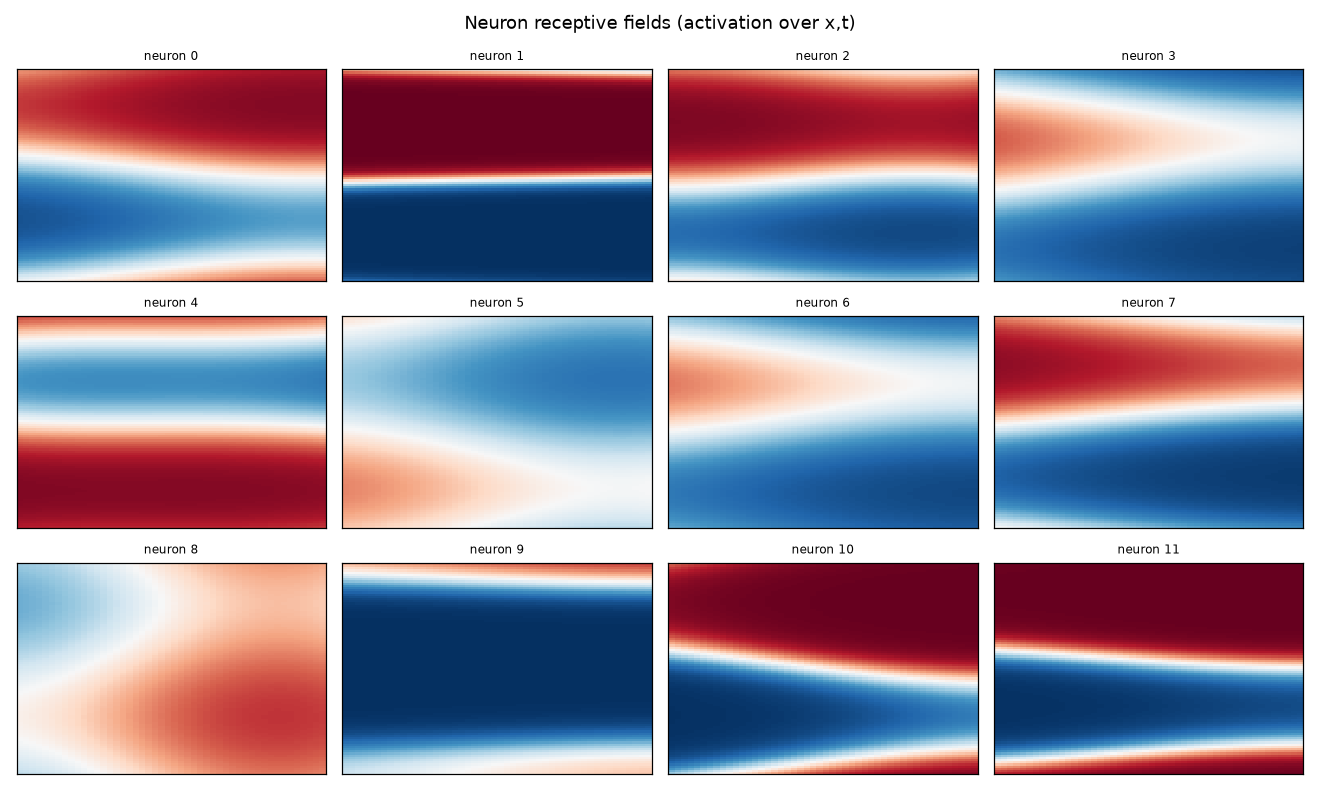
\includegraphics[width=\textwidth]{abl_ent_none/figures/neurons.png}
\caption{\textbf{abl\_ent\_none} --- Classical post-net neurons: receptive fields over $(x,t)$ and each neuron's dominant spatial frequency / effective rank.}
\end{figure}
\begin{figure}[H]\centering
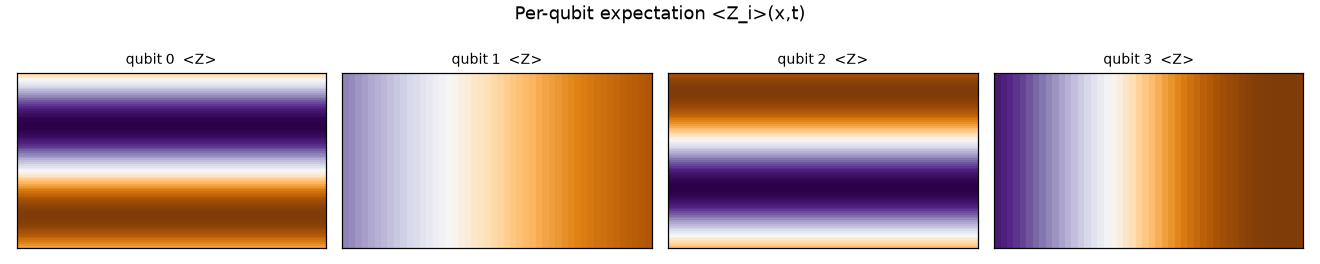
\includegraphics[width=\textwidth]{abl_ent_none/figures/qubits.png}
\caption{\textbf{abl\_ent\_none} --- Per-qubit $\langle Z\rangle$ receptive fields --- what feature each qubit computes over the domain (quantum models only).}
\end{figure}
\begin{figure}[H]\centering
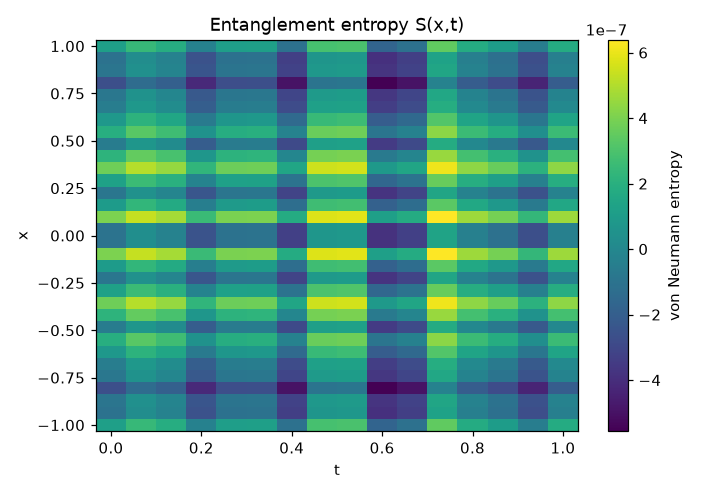
\includegraphics[width=\textwidth]{abl_ent_none/figures/entanglement.png}
\caption{\textbf{abl\_ent\_none} --- Von Neumann entanglement entropy $S(x,t)$ of a qubit bipartition across the domain (quantum models only).}
\end{figure}
\begin{figure}[H]\centering
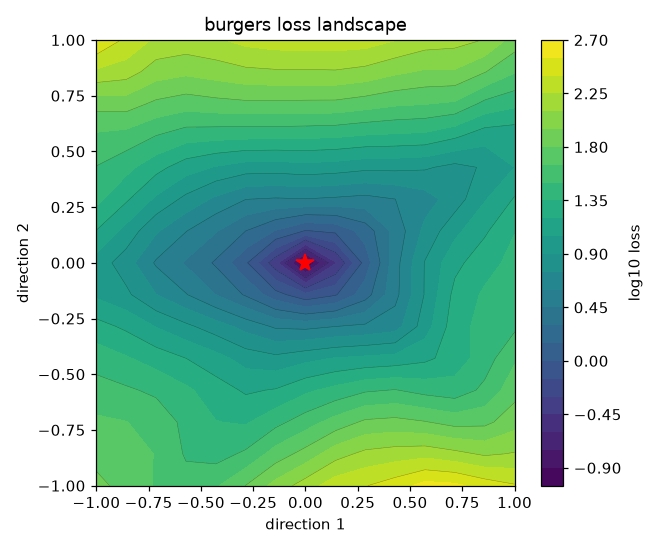
\includegraphics[width=\textwidth]{abl_ent_none/figures/landscape.png}
\caption{\textbf{abl\_ent\_none} --- Filter-normalized 2-D loss landscape around the trained minimum (Li et al.\ 2018). Flat/wide vs.\ sharp basin.}
\end{figure}
\begin{figure}[H]\centering
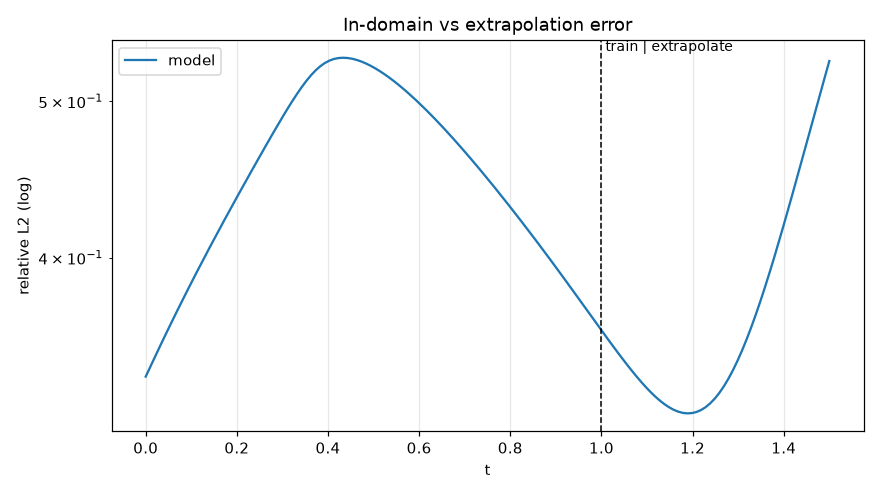
\includegraphics[width=\textwidth]{abl_ent_none/figures/generalization.png}
\caption{\textbf{abl\_ent\_none} --- Extrapolation: relative $L_2$ vs.\ $t$ beyond the $t\in[0,1]$ training window --- the off-domain penalty.}
\end{figure}
\begin{figure}[H]\centering
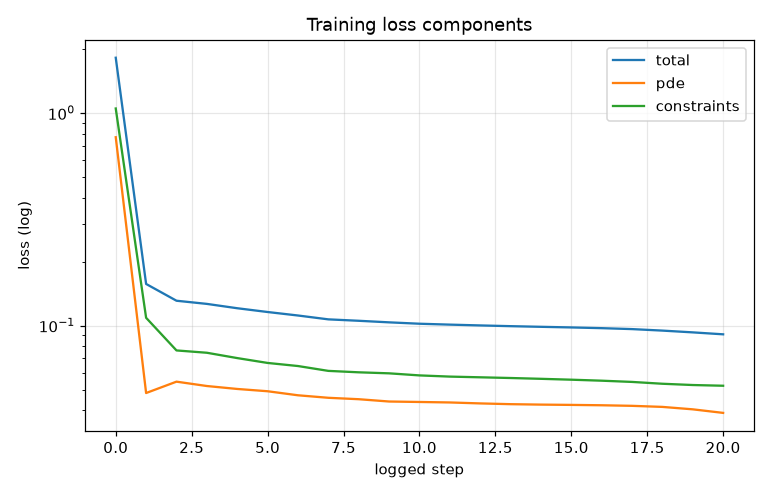
\includegraphics[width=\textwidth]{abl_ent_none/figures/loss.png}
\caption{\textbf{abl\_ent\_none} --- Training loss history (total, PDE-residual, and constraint terms).}
\end{figure}
\clearpage
\subsection{abl\_ent\_ring}
\noindent\small \textbf{rel-$L_2$}: 0.4851  \textbf{params}: 121  \textbf{PDE}: burgers  \textbf{Adam iters}: 2000  \textbf{seed}: 0  \textbf{model}: qapinn  \textbf{final PDE loss}: 4.16e-02  \textbf{wall time (s)}: 1887  \textbf{VQC}: 4q x3L ent=ring meas=multi scale=1.0\normalsize

\noindent\textbf{Observation.} Prediction again caps near +/-0.6 with the same shock-band error structure (|error| \textasciitilde{}0.9 along x=0), and the slice plots show the smooth model curve missing the sharp jump identically to the none run. Spectrum matches reference at k=1-2 then rolls off, model bars sitting \textasciitilde{}1 order below reference by k\textasciitilde{}10. Critically the entanglement entropy is now substantial and non-trivial, ranging roughly 0.62-1.25 von Neumann units with a smooth spatial pattern (high entropy \textasciitilde{}1.2 in the upper-left x\textgreater{}0.5/t\textless{}0.3 region, a dark low-entropy pocket \textasciitilde{}0.65 near x\textasciitilde{}-0.5/t\textasciitilde{}0). The loss landscape shows a well-defined minimum but with a secondary basin toward the lower-left, and F-principle 'iter to halve' sits at \textasciitilde{}250. Inference: ring entanglement switches the circuit into a genuinely entangled regime (S\textasciitilde{}1), yet the shock fit is essentially unchanged from none, suggesting the entangler adds correlation without improving expressivity for this discontinuity.

\begin{figure}[H]\centering
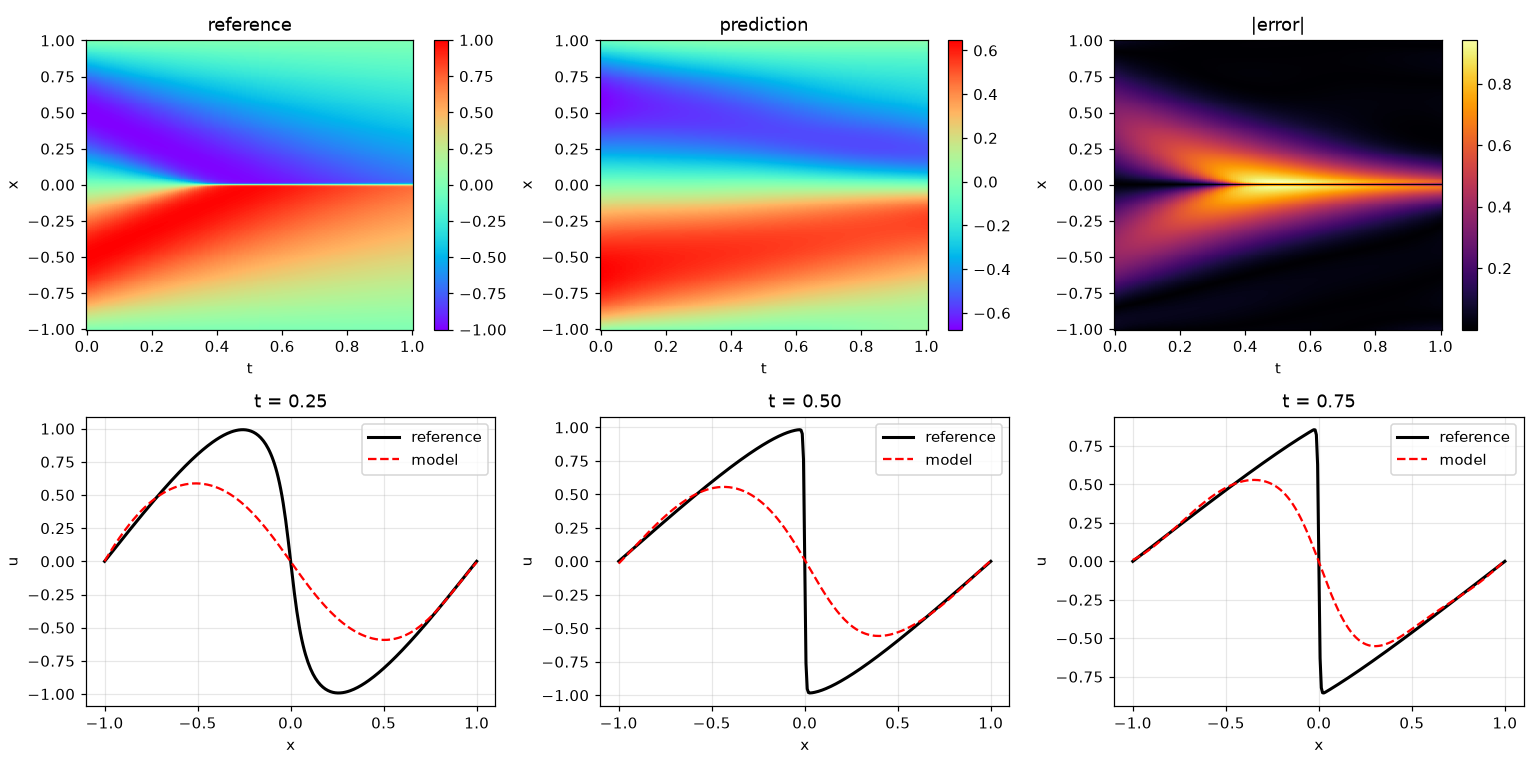
\includegraphics[width=\textwidth]{abl_ent_ring/figures/solution.png}
\caption{\textbf{abl\_ent\_ring} --- Predicted field $u(x,t)$ vs.\ exact reference, with the pointwise error map. The shock ($x\!=\!0$) is where a smooth network struggles.}
\end{figure}
\begin{figure}[H]\centering
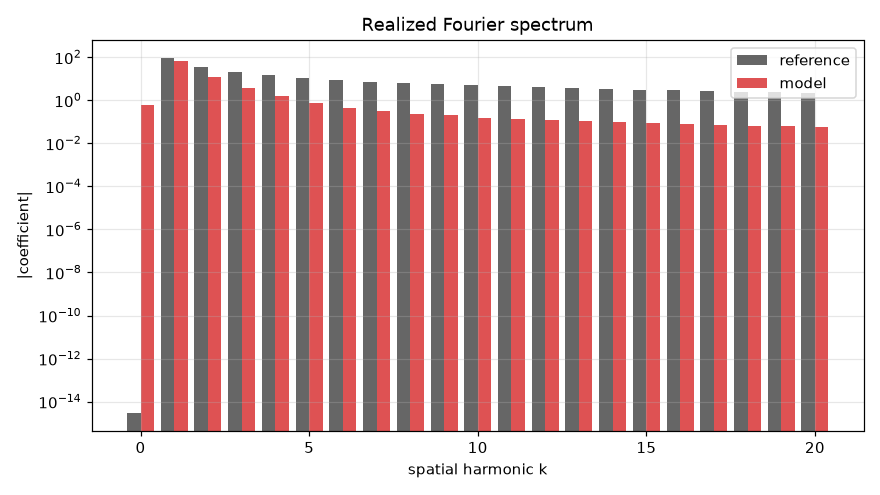
\includegraphics[width=\textwidth]{abl_ent_ring/figures/spectrum.png}
\caption{\textbf{abl\_ent\_ring} --- Realized spatial spectrum (per-harmonic magnitude) vs.\ reference. Tests whether the model captures the high-$k$ shock tail or only low frequencies.}
\end{figure}
\begin{figure}[H]\centering
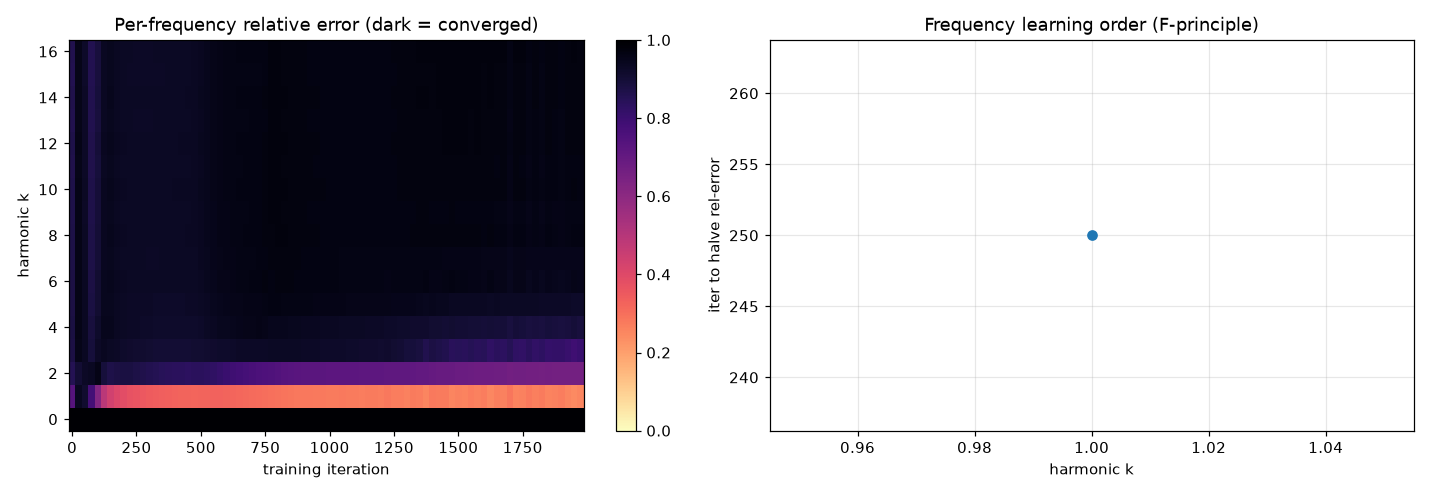
\includegraphics[width=\textwidth]{abl_ent_ring/figures/fprinciple.png}
\caption{\textbf{abl\_ent\_ring} --- F-principle heat-map: iteration at which each harmonic's relative error halves. Low harmonics converging first is the F-principle signature.}
\end{figure}
\begin{figure}[H]\centering
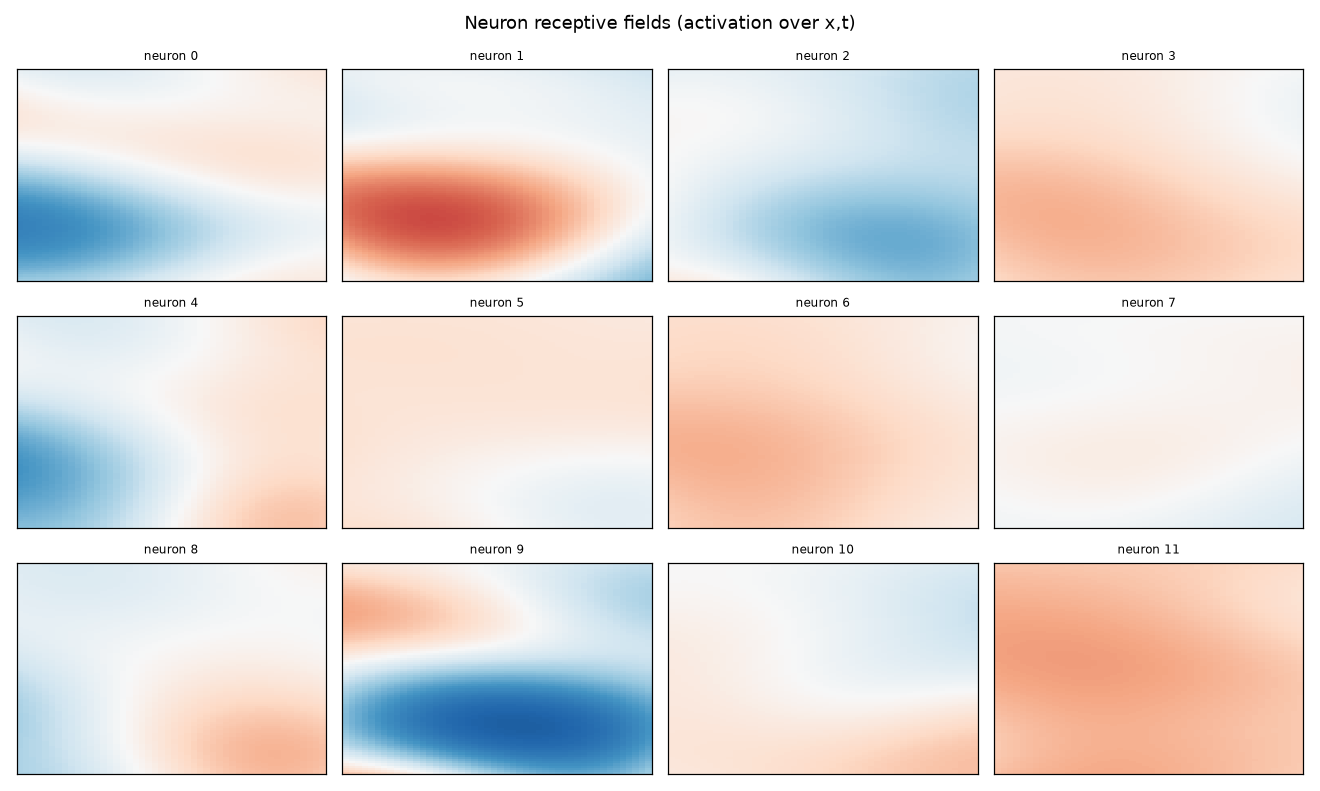
\includegraphics[width=\textwidth]{abl_ent_ring/figures/neurons.png}
\caption{\textbf{abl\_ent\_ring} --- Classical post-net neurons: receptive fields over $(x,t)$ and each neuron's dominant spatial frequency / effective rank.}
\end{figure}
\begin{figure}[H]\centering
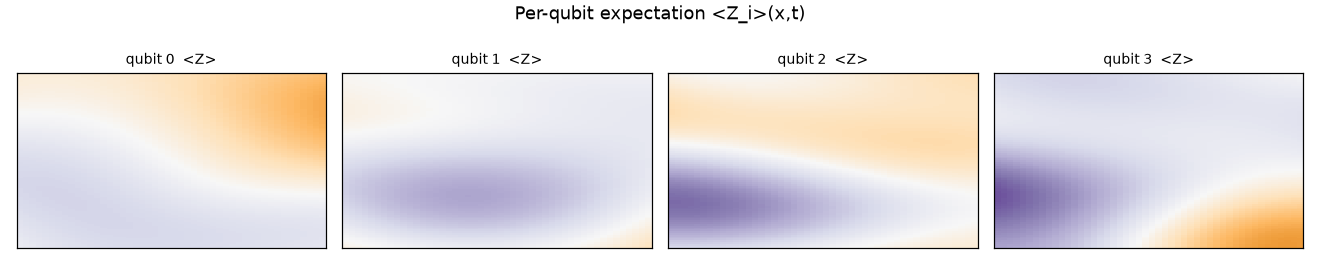
\includegraphics[width=\textwidth]{abl_ent_ring/figures/qubits.png}
\caption{\textbf{abl\_ent\_ring} --- Per-qubit $\langle Z\rangle$ receptive fields --- what feature each qubit computes over the domain (quantum models only).}
\end{figure}
\begin{figure}[H]\centering
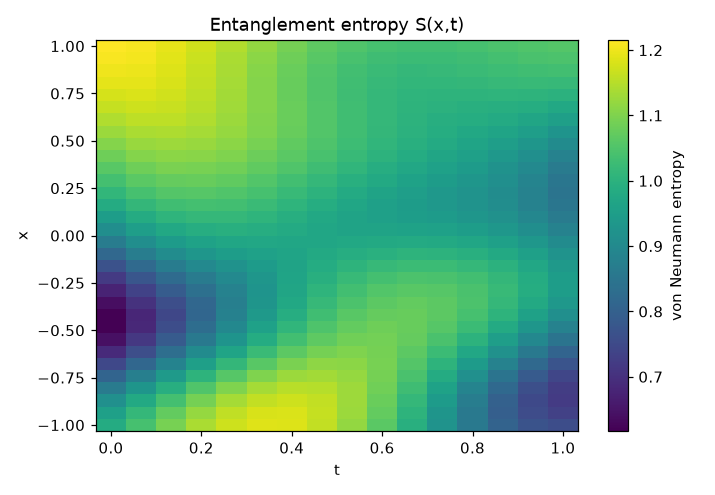
\includegraphics[width=\textwidth]{abl_ent_ring/figures/entanglement.png}
\caption{\textbf{abl\_ent\_ring} --- Von Neumann entanglement entropy $S(x,t)$ of a qubit bipartition across the domain (quantum models only).}
\end{figure}
\begin{figure}[H]\centering
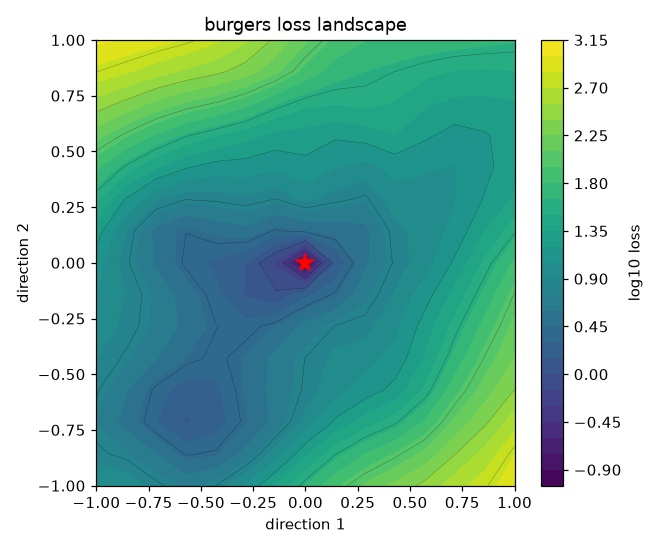
\includegraphics[width=\textwidth]{abl_ent_ring/figures/landscape.png}
\caption{\textbf{abl\_ent\_ring} --- Filter-normalized 2-D loss landscape around the trained minimum (Li et al.\ 2018). Flat/wide vs.\ sharp basin.}
\end{figure}
\begin{figure}[H]\centering
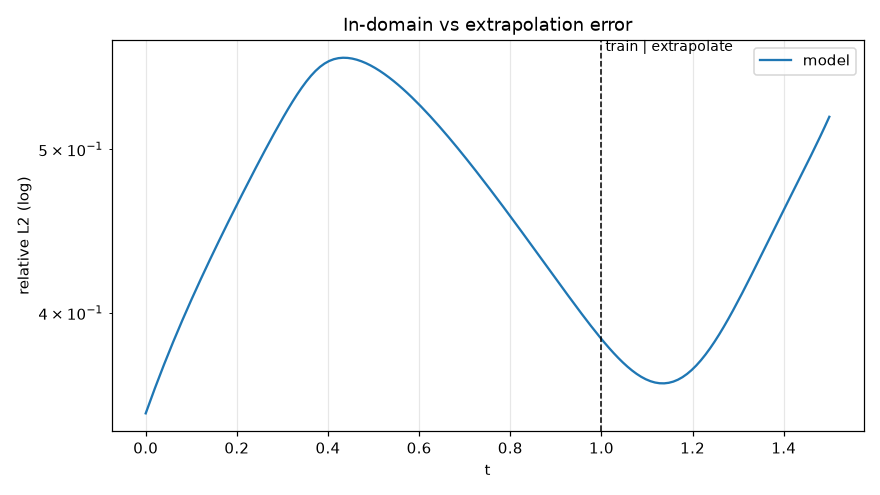
\includegraphics[width=\textwidth]{abl_ent_ring/figures/generalization.png}
\caption{\textbf{abl\_ent\_ring} --- Extrapolation: relative $L_2$ vs.\ $t$ beyond the $t\in[0,1]$ training window --- the off-domain penalty.}
\end{figure}
\begin{figure}[H]\centering
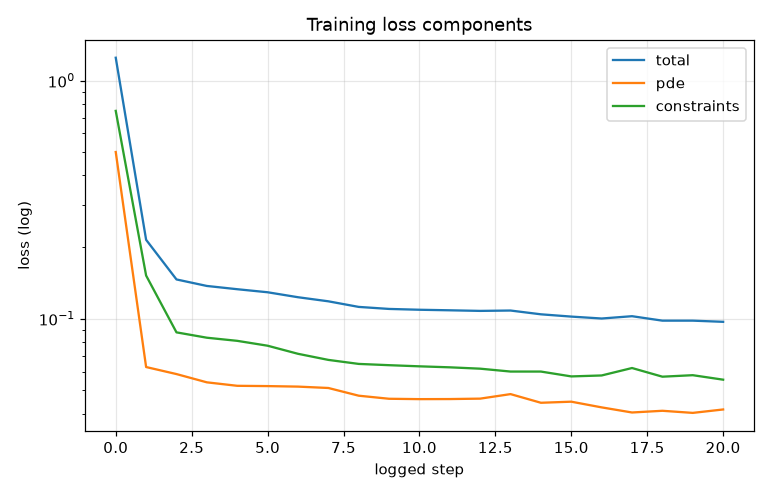
\includegraphics[width=\textwidth]{abl_ent_ring/figures/loss.png}
\caption{\textbf{abl\_ent\_ring} --- Training loss history (total, PDE-residual, and constraint terms).}
\end{figure}
\clearpage
\subsection{abl\_ent\_all\_to\_all}
\noindent\small \textbf{rel-$L_2$}: 0.4879  \textbf{params}: 121  \textbf{PDE}: burgers  \textbf{Adam iters}: 2000  \textbf{seed}: 0  \textbf{model}: qapinn  \textbf{final PDE loss}: 4.20e-02  \textbf{wall time (s)}: 1848  \textbf{VQC}: 4q x3L ent=all\_to\_all meas=multi scale=1.0\normalsize

\noindent\textbf{Observation.} Prediction caps \textasciitilde{}+/-0.65 with the familiar x=0 shock error band (\textasciitilde{}0.9), and slices show the same rounded-peak, no-jump behavior. Spectrum tracks reference to k\textasciitilde{}2 then the model falls below, \textasciitilde{}1 order down by k\textasciitilde{}10. Entanglement entropy is moderate, \textasciitilde{}0.45-1.05, with a distinctive smooth structure: a low-entropy dip (\textasciitilde{}0.45) centered at x\textasciitilde{}0.1/t\textasciitilde{}0.5 and higher entropy (\textasciitilde{}1.0) at the corners/edges (bottom-right t\textasciitilde{}1). Notably the extrapolation curve is the worst of the entanglement set, rising past relative-L2 = 1.0 by t=1.5 (vs \textasciitilde{}0.5-0.6 for none/ring), and F-principle iter-to-halve is highest at \textasciitilde{}575. Inference: full all-to-all connectivity produces the strongest entanglement gradients but the poorest temporal extrapolation and slowest frequency convergence, indicating the denser entangler over-parameterizes/harms generalization without fixing the in-domain shock.

\begin{figure}[H]\centering
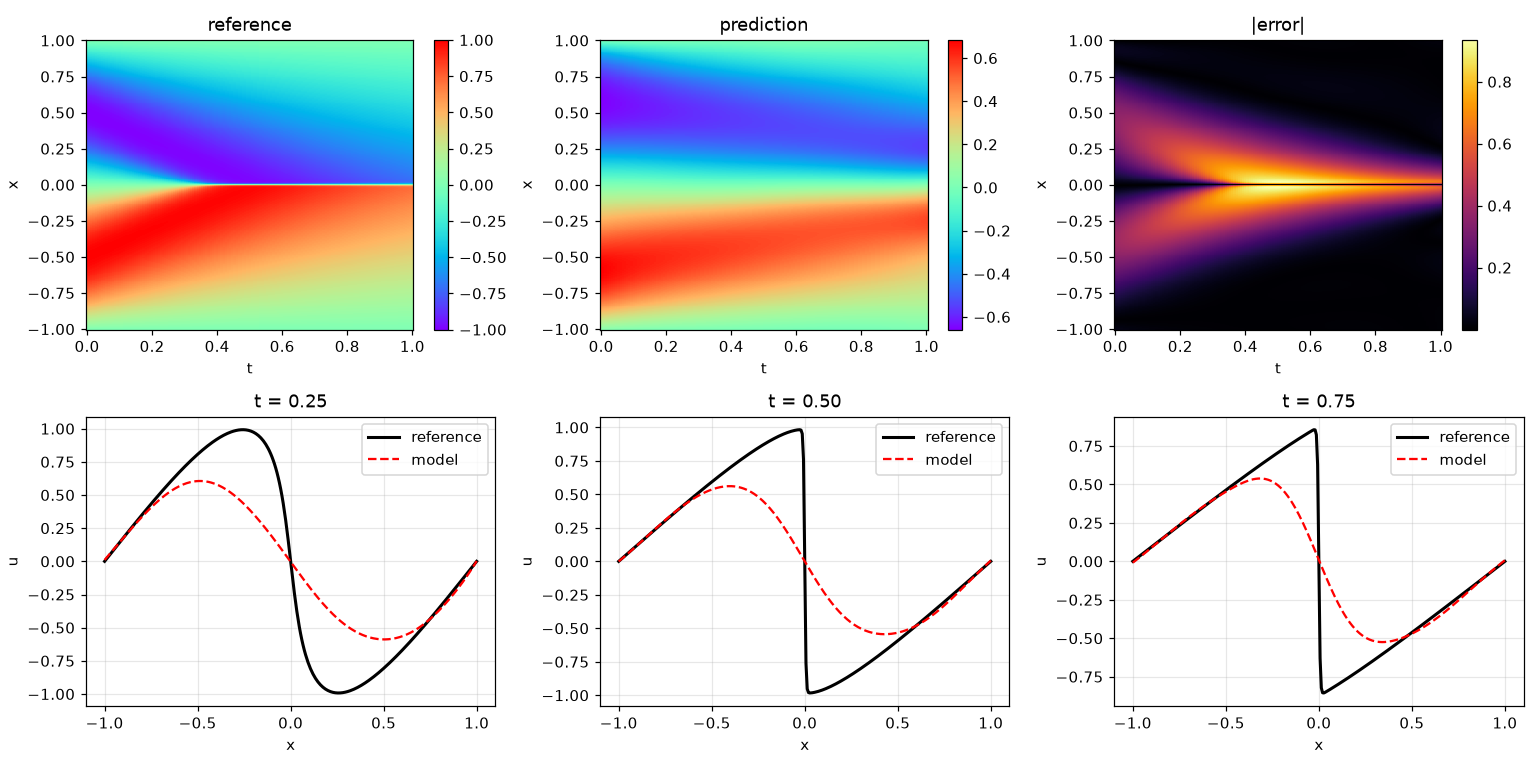
\includegraphics[width=\textwidth]{abl_ent_all_to_all/figures/solution.png}
\caption{\textbf{abl\_ent\_all\_to\_all} --- Predicted field $u(x,t)$ vs.\ exact reference, with the pointwise error map. The shock ($x\!=\!0$) is where a smooth network struggles.}
\end{figure}
\begin{figure}[H]\centering
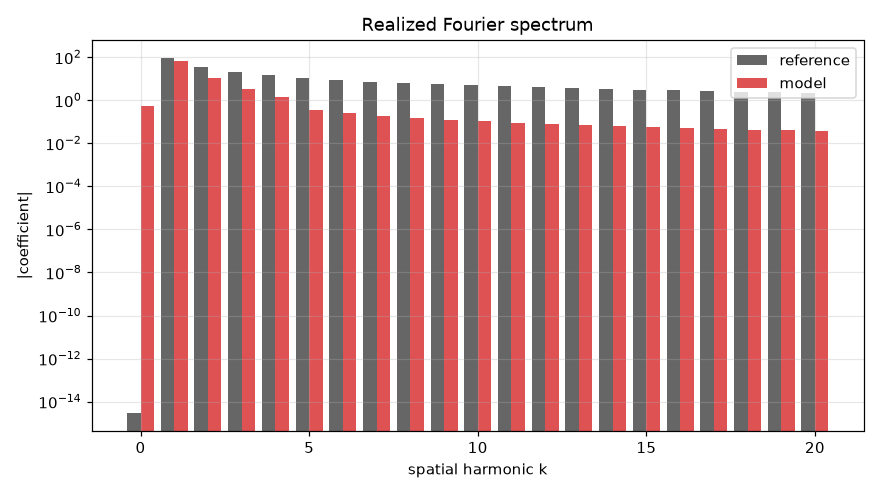
\includegraphics[width=\textwidth]{abl_ent_all_to_all/figures/spectrum.png}
\caption{\textbf{abl\_ent\_all\_to\_all} --- Realized spatial spectrum (per-harmonic magnitude) vs.\ reference. Tests whether the model captures the high-$k$ shock tail or only low frequencies.}
\end{figure}
\begin{figure}[H]\centering
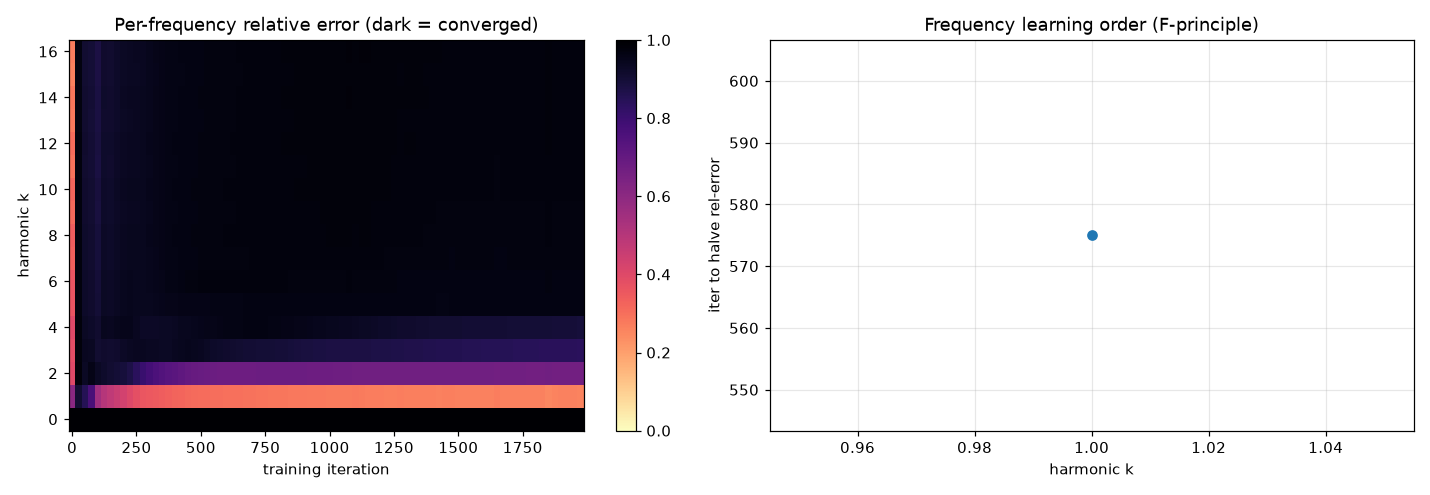
\includegraphics[width=\textwidth]{abl_ent_all_to_all/figures/fprinciple.png}
\caption{\textbf{abl\_ent\_all\_to\_all} --- F-principle heat-map: iteration at which each harmonic's relative error halves. Low harmonics converging first is the F-principle signature.}
\end{figure}
\begin{figure}[H]\centering
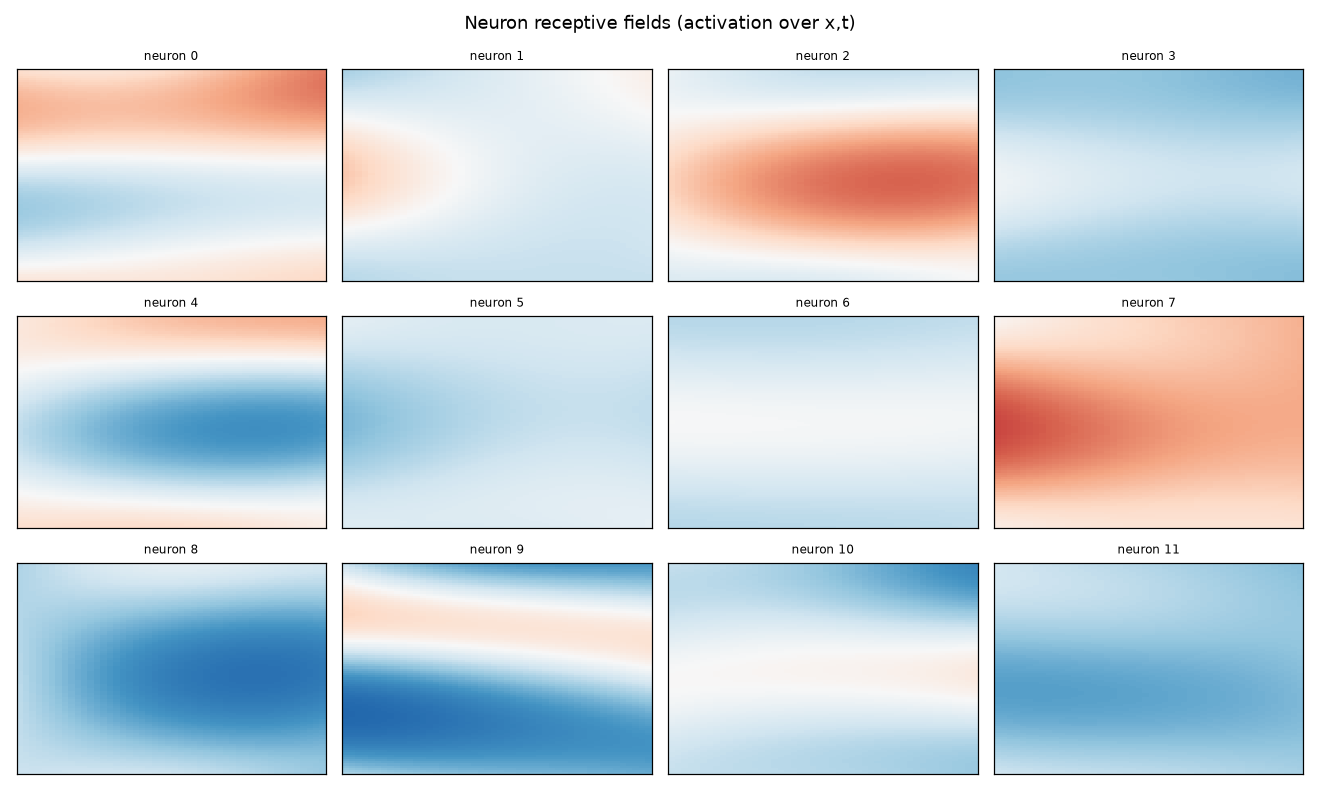
\includegraphics[width=\textwidth]{abl_ent_all_to_all/figures/neurons.png}
\caption{\textbf{abl\_ent\_all\_to\_all} --- Classical post-net neurons: receptive fields over $(x,t)$ and each neuron's dominant spatial frequency / effective rank.}
\end{figure}
\begin{figure}[H]\centering
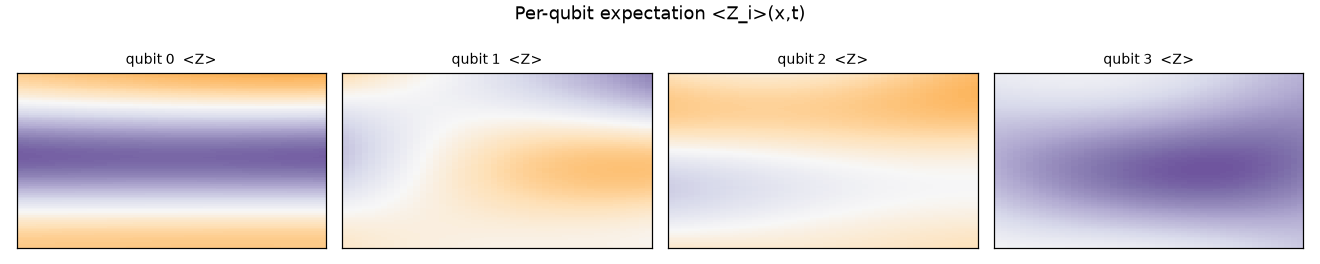
\includegraphics[width=\textwidth]{abl_ent_all_to_all/figures/qubits.png}
\caption{\textbf{abl\_ent\_all\_to\_all} --- Per-qubit $\langle Z\rangle$ receptive fields --- what feature each qubit computes over the domain (quantum models only).}
\end{figure}
\begin{figure}[H]\centering
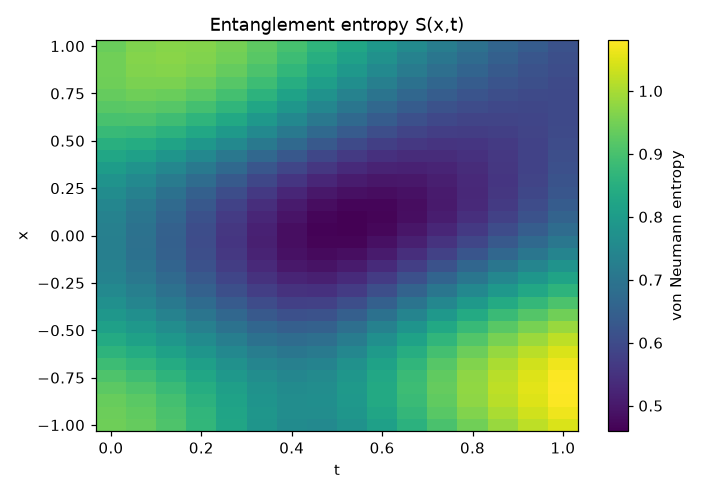
\includegraphics[width=\textwidth]{abl_ent_all_to_all/figures/entanglement.png}
\caption{\textbf{abl\_ent\_all\_to\_all} --- Von Neumann entanglement entropy $S(x,t)$ of a qubit bipartition across the domain (quantum models only).}
\end{figure}
\begin{figure}[H]\centering
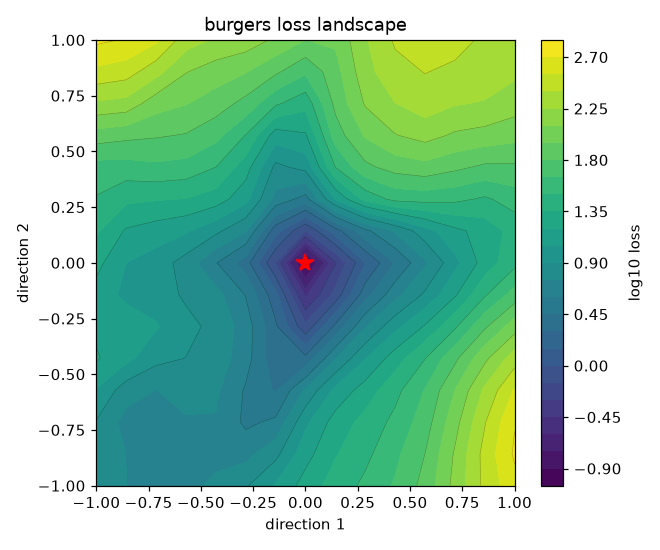
\includegraphics[width=\textwidth]{abl_ent_all_to_all/figures/landscape.png}
\caption{\textbf{abl\_ent\_all\_to\_all} --- Filter-normalized 2-D loss landscape around the trained minimum (Li et al.\ 2018). Flat/wide vs.\ sharp basin.}
\end{figure}
\begin{figure}[H]\centering
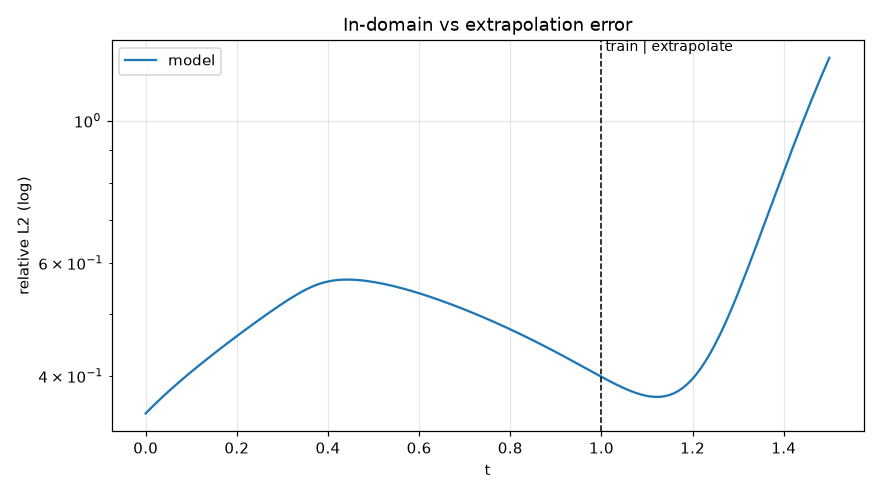
\includegraphics[width=\textwidth]{abl_ent_all_to_all/figures/generalization.png}
\caption{\textbf{abl\_ent\_all\_to\_all} --- Extrapolation: relative $L_2$ vs.\ $t$ beyond the $t\in[0,1]$ training window --- the off-domain penalty.}
\end{figure}
\begin{figure}[H]\centering
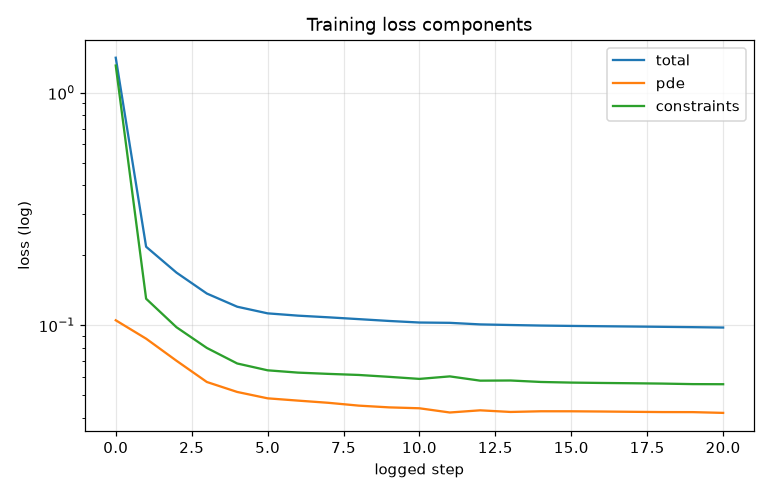
\includegraphics[width=\textwidth]{abl_ent_all_to_all/figures/loss.png}
\caption{\textbf{abl\_ent\_all\_to\_all} --- Training loss history (total, PDE-residual, and constraint terms).}
\end{figure}
\clearpage
\section{Tier-1 ablation --- post-net width}
How much classical readout the VQC needs. $[16]$ is the reference run.

\subsection{abl\_post\_lin}
\noindent\small \textbf{rel-$L_2$}: 0.5439  \textbf{params}: 29  \textbf{PDE}: burgers  \textbf{Adam iters}: 2000  \textbf{seed}: 0  \textbf{model}: qapinn  \textbf{final PDE loss}: 4.97e-02  \textbf{wall time (s)}: 1639  \textbf{VQC}: 4q x3L ent=linear meas=multi scale=1.0\normalsize

\noindent\textbf{Observation.} With no hidden post-net ([]), the prediction cap drops to the lowest \textasciitilde{}+/-0.55 and the error band at x=0 is correspondingly the most pronounced; slices show the flattest, most under-amplitude model curves of the post series. Spectrum matches k=1-2 then rolls off \textasciitilde{}1 order by k\textasciitilde{}10, similar shape to baseline. Entanglement entropy ranges \textasciitilde{}0.6-1.15 with a yellow high-entropy blob at x\textasciitilde{}0.4/t\textasciitilde{}0.9 and a dark low pocket \textasciitilde{}0.6 at x\textasciitilde{}-0.3/t\textasciitilde{}0. The F-principle right panel is EMPTY (no data point plotted, axes autoscaled to +/-0.05), and the per-frequency heatmap shows only k=0-2 with slow red convergence. Inference: removing the classical post-net (linear readout only) yields the weakest amplitude fit, confirming the post-net is what lets the model push output amplitude toward the reference; the missing F-principle marker suggests the halving metric failed/never triggered here.

\begin{figure}[H]\centering
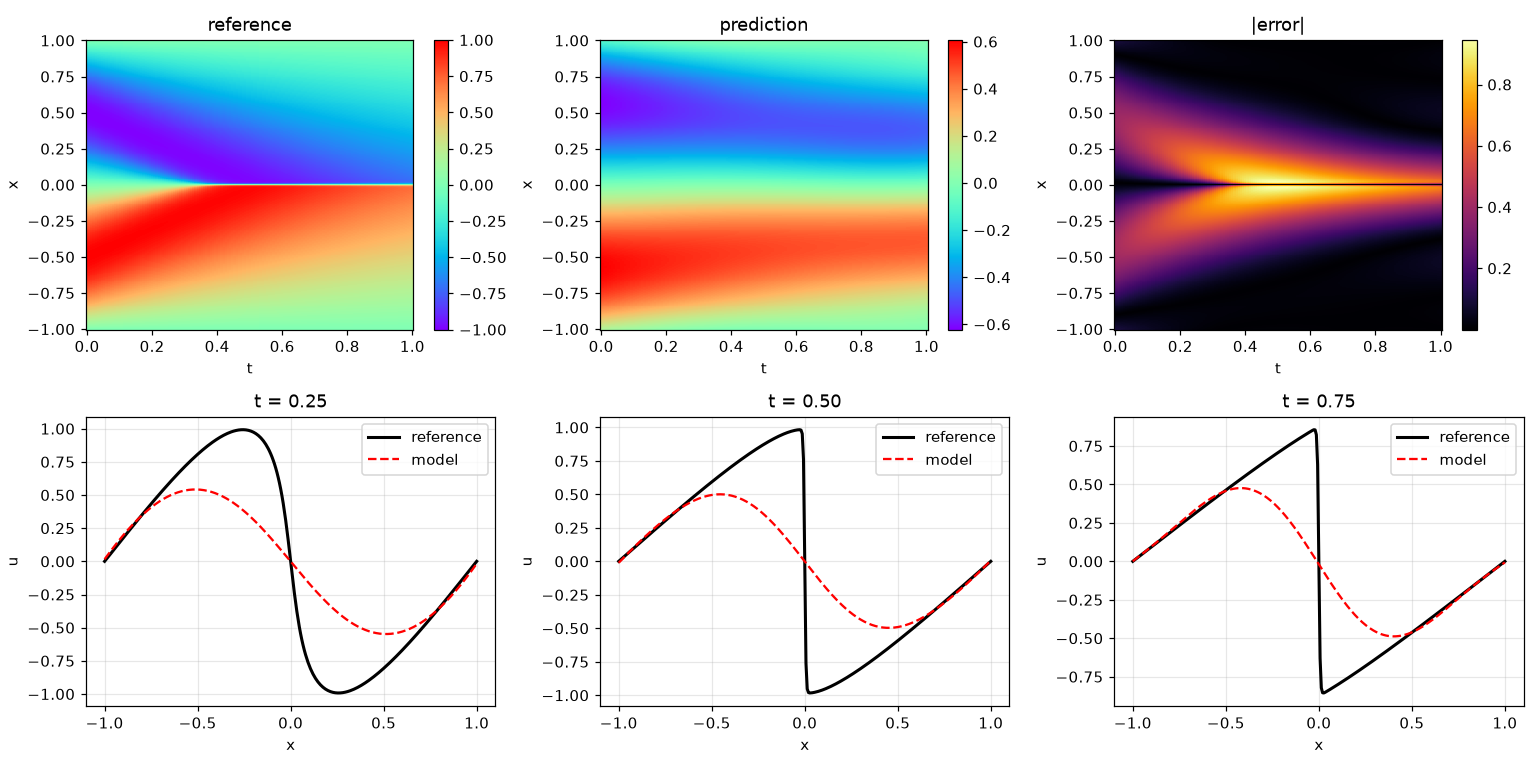
\includegraphics[width=\textwidth]{abl_post_lin/figures/solution.png}
\caption{\textbf{abl\_post\_lin} --- Predicted field $u(x,t)$ vs.\ exact reference, with the pointwise error map. The shock ($x\!=\!0$) is where a smooth network struggles.}
\end{figure}
\begin{figure}[H]\centering
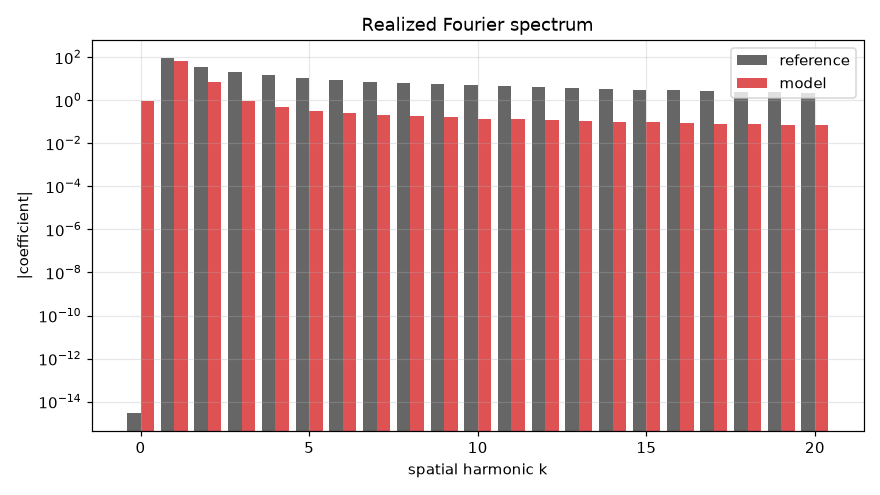
\includegraphics[width=\textwidth]{abl_post_lin/figures/spectrum.png}
\caption{\textbf{abl\_post\_lin} --- Realized spatial spectrum (per-harmonic magnitude) vs.\ reference. Tests whether the model captures the high-$k$ shock tail or only low frequencies.}
\end{figure}
\begin{figure}[H]\centering
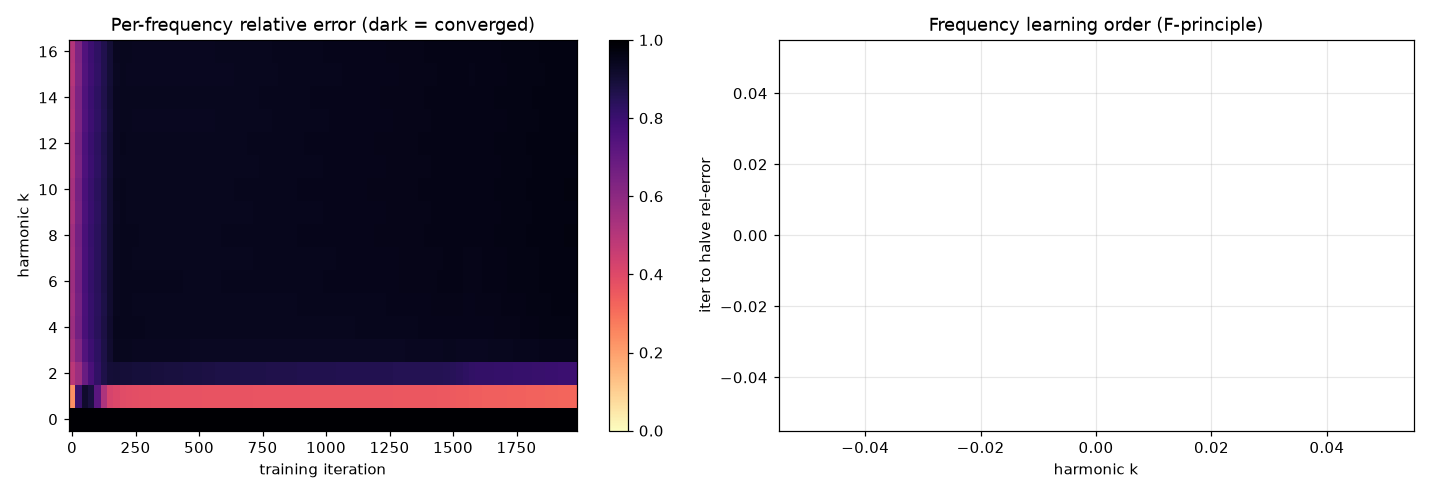
\includegraphics[width=\textwidth]{abl_post_lin/figures/fprinciple.png}
\caption{\textbf{abl\_post\_lin} --- F-principle heat-map: iteration at which each harmonic's relative error halves. Low harmonics converging first is the F-principle signature.}
\end{figure}
\begin{figure}[H]\centering
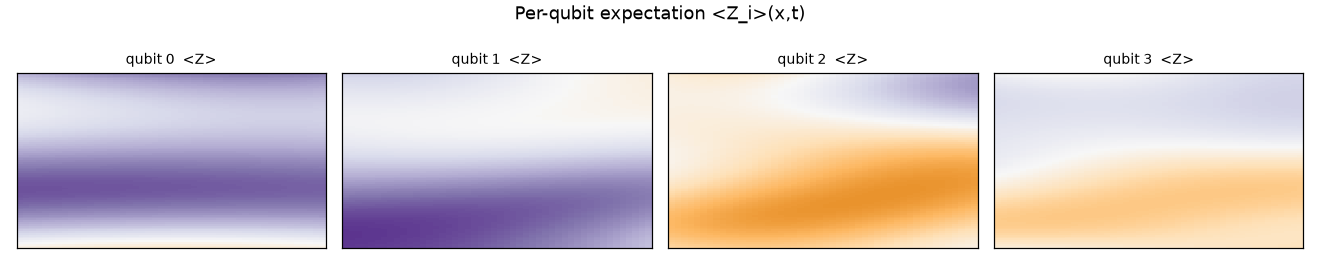
\includegraphics[width=\textwidth]{abl_post_lin/figures/qubits.png}
\caption{\textbf{abl\_post\_lin} --- Per-qubit $\langle Z\rangle$ receptive fields --- what feature each qubit computes over the domain (quantum models only).}
\end{figure}
\begin{figure}[H]\centering
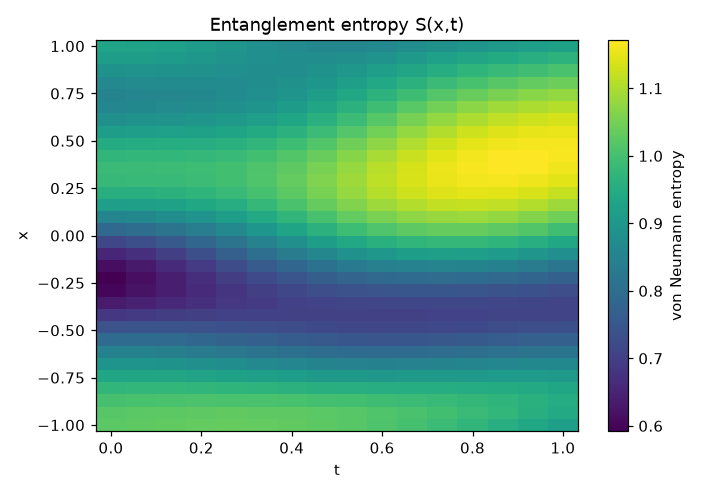
\includegraphics[width=\textwidth]{abl_post_lin/figures/entanglement.png}
\caption{\textbf{abl\_post\_lin} --- Von Neumann entanglement entropy $S(x,t)$ of a qubit bipartition across the domain (quantum models only).}
\end{figure}
\begin{figure}[H]\centering
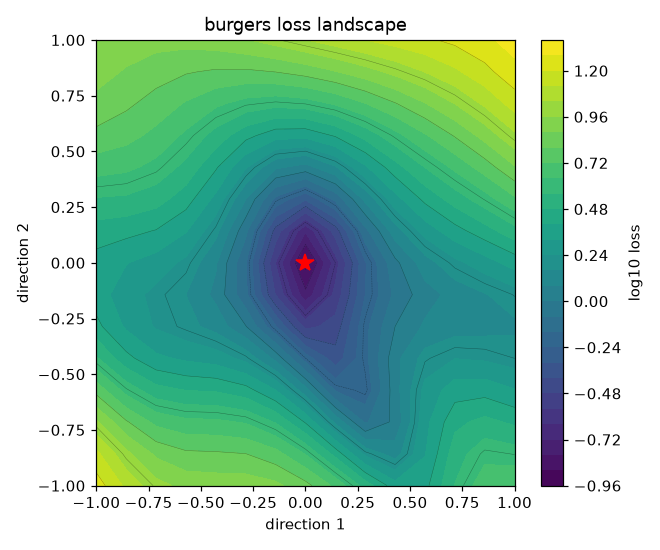
\includegraphics[width=\textwidth]{abl_post_lin/figures/landscape.png}
\caption{\textbf{abl\_post\_lin} --- Filter-normalized 2-D loss landscape around the trained minimum (Li et al.\ 2018). Flat/wide vs.\ sharp basin.}
\end{figure}
\begin{figure}[H]\centering
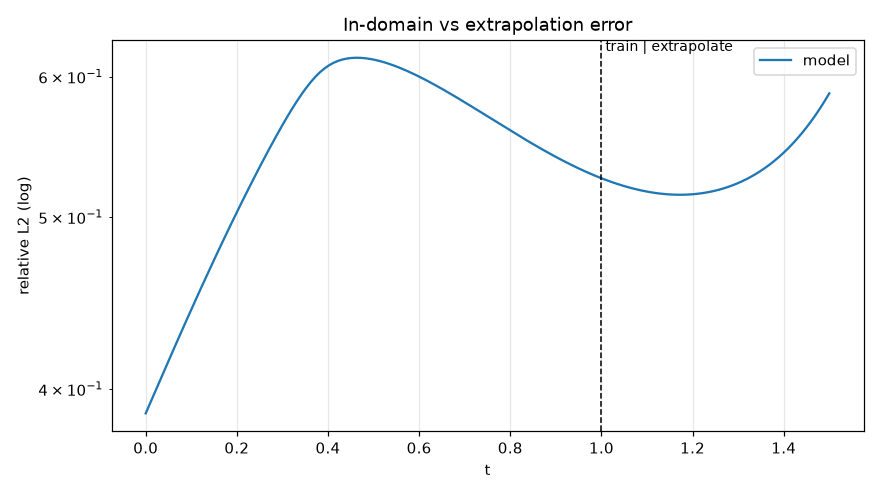
\includegraphics[width=\textwidth]{abl_post_lin/figures/generalization.png}
\caption{\textbf{abl\_post\_lin} --- Extrapolation: relative $L_2$ vs.\ $t$ beyond the $t\in[0,1]$ training window --- the off-domain penalty.}
\end{figure}
\begin{figure}[H]\centering
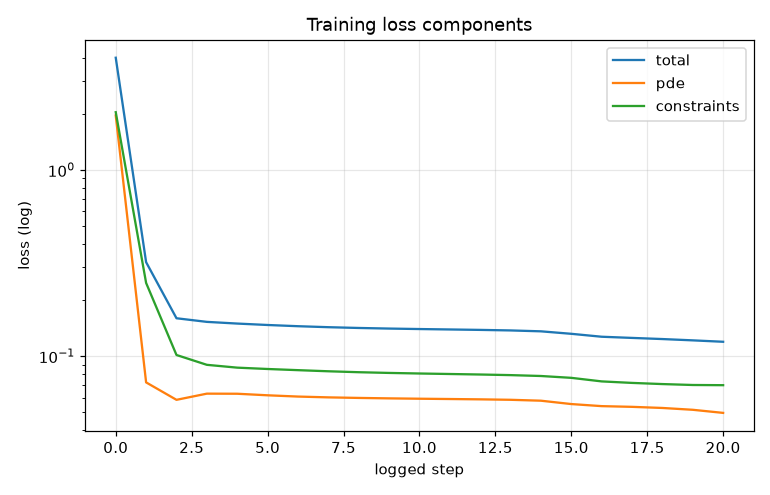
\includegraphics[width=\textwidth]{abl_post_lin/figures/loss.png}
\caption{\textbf{abl\_post\_lin} --- Training loss history (total, PDE-residual, and constraint terms).}
\end{figure}
\clearpage
\subsection{abl\_post\_8}
\noindent\small \textbf{rel-$L_2$}: 0.4775  \textbf{params}: 73  \textbf{PDE}: burgers  \textbf{Adam iters}: 2000  \textbf{seed}: 0  \textbf{model}: qapinn  \textbf{final PDE loss}: 4.13e-02  \textbf{wall time (s)}: 1680  \textbf{VQC}: 4q x3L ent=linear meas=multi scale=1.0\normalsize

\noindent\textbf{Observation.} Prediction cap recovers to \textasciitilde{}+/-0.63 (higher than post\_lin), and the slice fits are visibly the best-amplitude of the series, with the model curve reaching \textasciitilde{}0.63 at t=0.25; error still bands at the x=0 shock (\textasciitilde{}0.9) but in-domain smooth regions fit tightly. Spectrum matches reference through k\textasciitilde{}2 then declines \textasciitilde{}1 order by k\textasciitilde{}10. Entanglement entropy \textasciitilde{}0.55-1.0 with a bright high-entropy lobe (\textasciitilde{}1.0) in the lower-left x\textless{}-0.25/t\textless{}0.4 and a dark low corner (\textasciitilde{}0.55) upper-left. This run shows the best generalization: extrapolation relative-L2 bottoms \textasciitilde{}0.42 right at the train|extrapolate boundary and only rises to \textasciitilde{}0.55 by t=1.5; neurons.png correctly shows 8 receptive fields. The F-principle right panel is again EMPTY. Inference: an 8-wide post-net already restores near-full amplitude and gives the tightest extrapolation, implying the post-net width delivers most of its benefit by width 8.

\begin{figure}[H]\centering
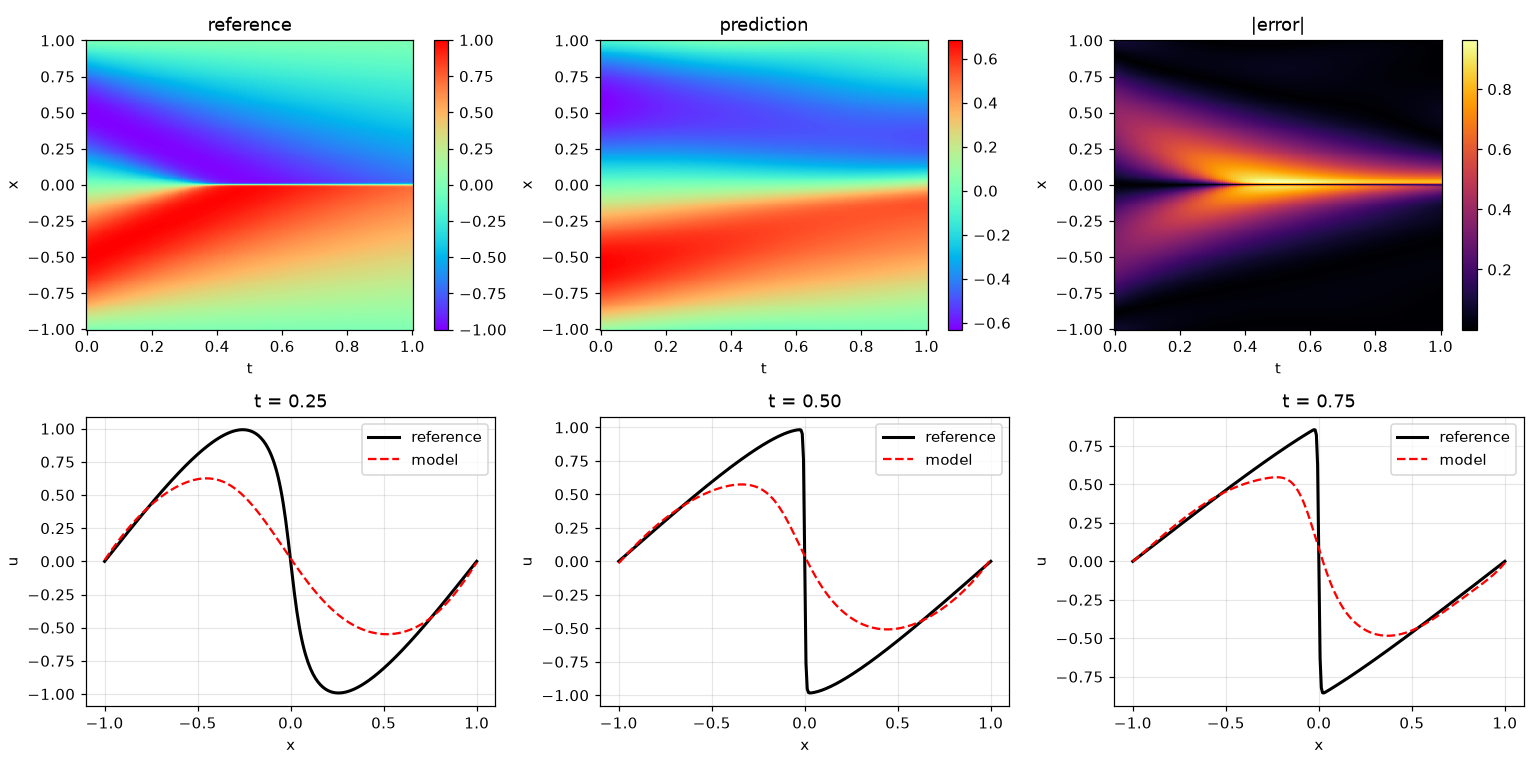
\includegraphics[width=\textwidth]{abl_post_8/figures/solution.png}
\caption{\textbf{abl\_post\_8} --- Predicted field $u(x,t)$ vs.\ exact reference, with the pointwise error map. The shock ($x\!=\!0$) is where a smooth network struggles.}
\end{figure}
\begin{figure}[H]\centering
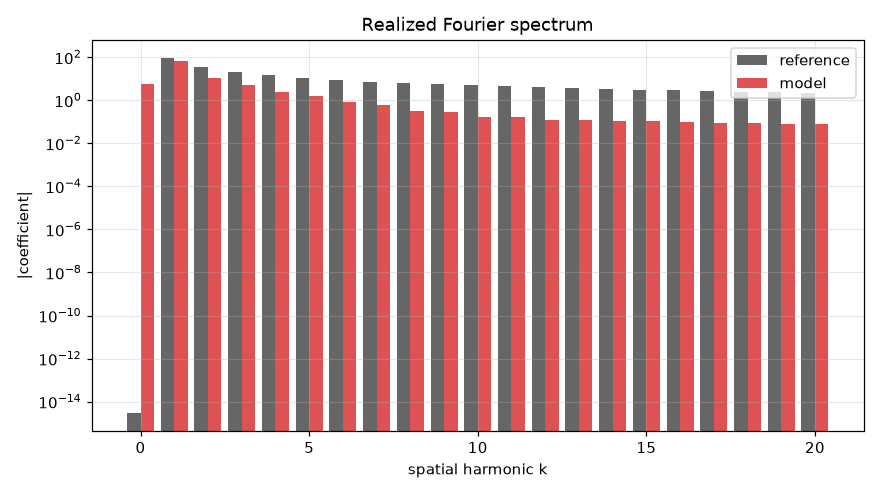
\includegraphics[width=\textwidth]{abl_post_8/figures/spectrum.png}
\caption{\textbf{abl\_post\_8} --- Realized spatial spectrum (per-harmonic magnitude) vs.\ reference. Tests whether the model captures the high-$k$ shock tail or only low frequencies.}
\end{figure}
\begin{figure}[H]\centering
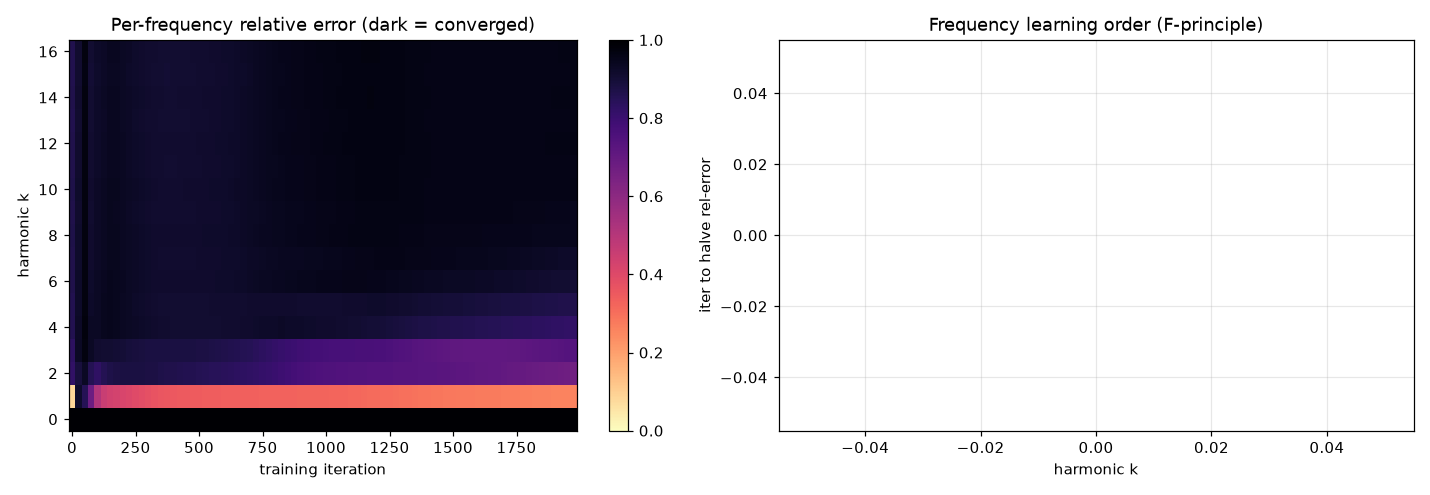
\includegraphics[width=\textwidth]{abl_post_8/figures/fprinciple.png}
\caption{\textbf{abl\_post\_8} --- F-principle heat-map: iteration at which each harmonic's relative error halves. Low harmonics converging first is the F-principle signature.}
\end{figure}
\begin{figure}[H]\centering
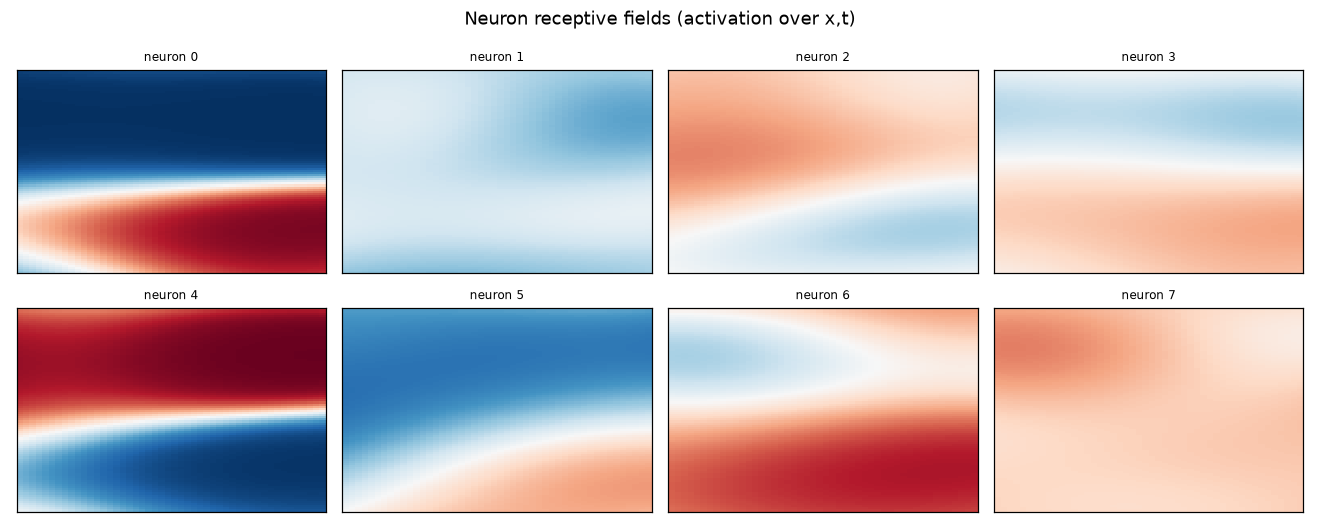
\includegraphics[width=\textwidth]{abl_post_8/figures/neurons.png}
\caption{\textbf{abl\_post\_8} --- Classical post-net neurons: receptive fields over $(x,t)$ and each neuron's dominant spatial frequency / effective rank.}
\end{figure}
\begin{figure}[H]\centering
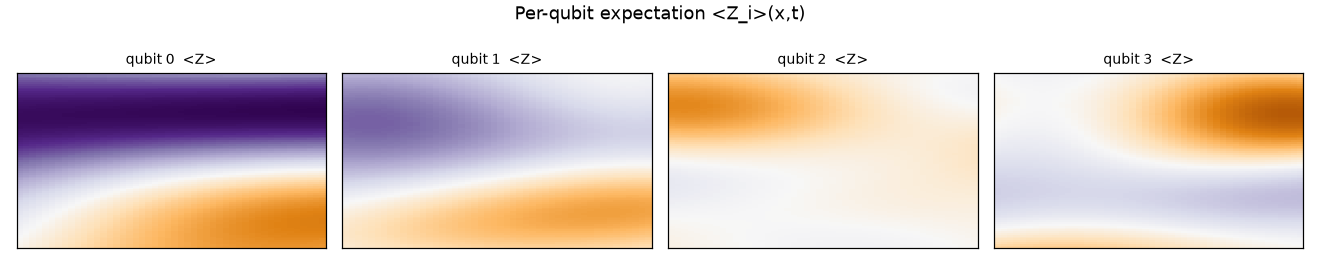
\includegraphics[width=\textwidth]{abl_post_8/figures/qubits.png}
\caption{\textbf{abl\_post\_8} --- Per-qubit $\langle Z\rangle$ receptive fields --- what feature each qubit computes over the domain (quantum models only).}
\end{figure}
\begin{figure}[H]\centering
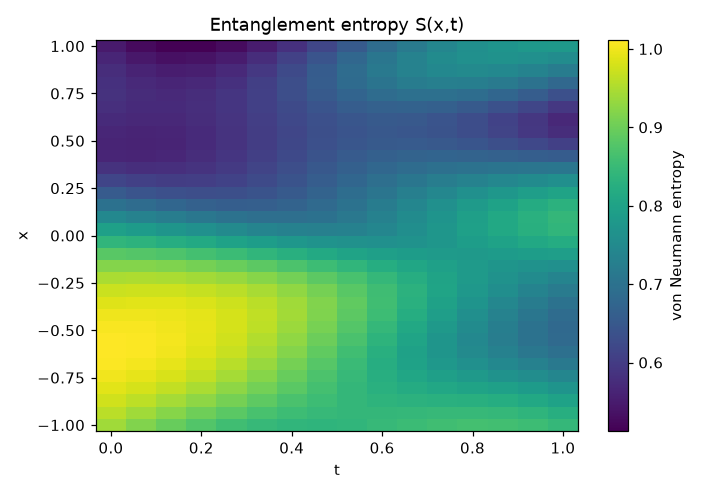
\includegraphics[width=\textwidth]{abl_post_8/figures/entanglement.png}
\caption{\textbf{abl\_post\_8} --- Von Neumann entanglement entropy $S(x,t)$ of a qubit bipartition across the domain (quantum models only).}
\end{figure}
\begin{figure}[H]\centering
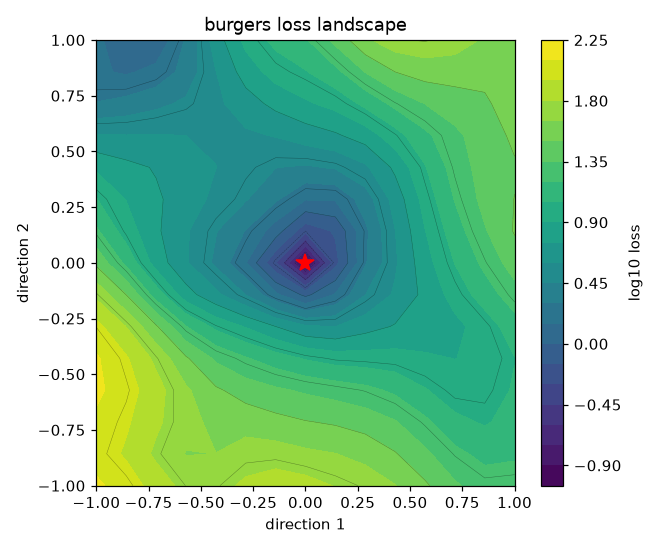
\includegraphics[width=\textwidth]{abl_post_8/figures/landscape.png}
\caption{\textbf{abl\_post\_8} --- Filter-normalized 2-D loss landscape around the trained minimum (Li et al.\ 2018). Flat/wide vs.\ sharp basin.}
\end{figure}
\begin{figure}[H]\centering
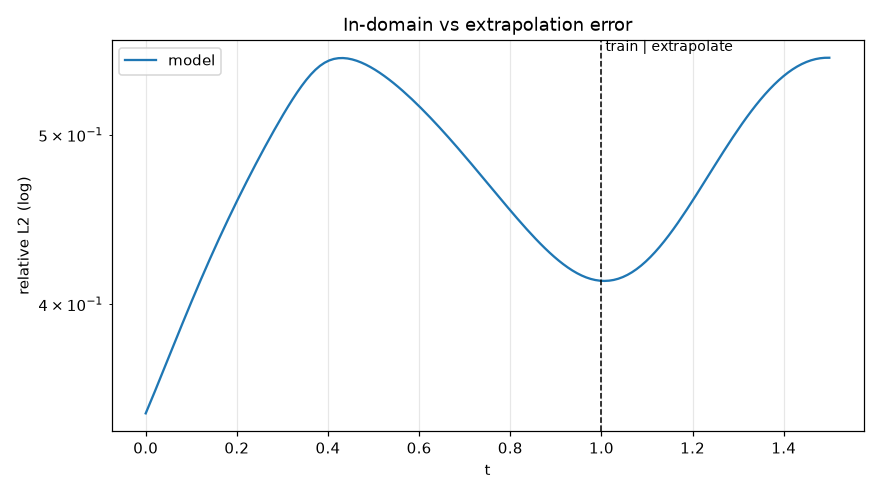
\includegraphics[width=\textwidth]{abl_post_8/figures/generalization.png}
\caption{\textbf{abl\_post\_8} --- Extrapolation: relative $L_2$ vs.\ $t$ beyond the $t\in[0,1]$ training window --- the off-domain penalty.}
\end{figure}
\begin{figure}[H]\centering
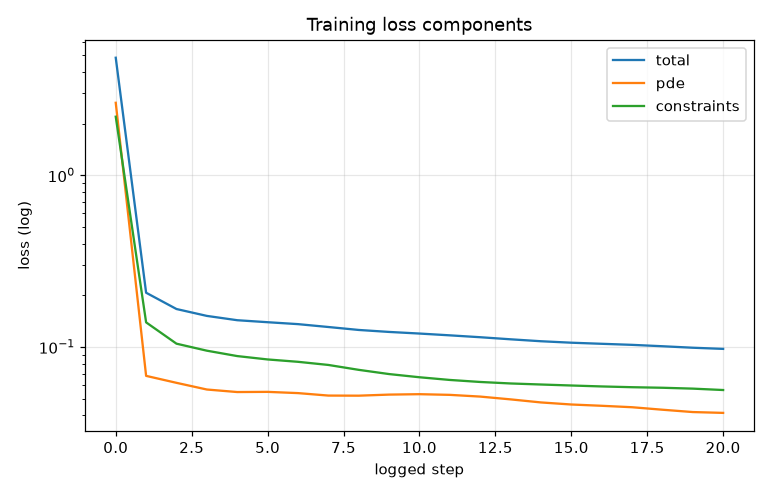
\includegraphics[width=\textwidth]{abl_post_8/figures/loss.png}
\caption{\textbf{abl\_post\_8} --- Training loss history (total, PDE-residual, and constraint terms).}
\end{figure}
\clearpage
\subsection{abl\_post\_32}
\noindent\small \textbf{rel-$L_2$}: 0.4658  \textbf{params}: 217  \textbf{PDE}: burgers  \textbf{Adam iters}: 2000  \textbf{seed}: 0  \textbf{model}: qapinn  \textbf{final PDE loss}: 3.98e-02  \textbf{wall time (s)}: 1707  \textbf{VQC}: 4q x3L ent=linear meas=multi scale=1.0\normalsize

\noindent\textbf{Observation.} Prediction cap \textasciitilde{}+/-0.63, comparable to post\_8 and the baseline, with the same x=0 shock error band (\textasciitilde{}0.9) and rounded-peak slices. Spectrum tracks reference to k\textasciitilde{}2 then rolls off \textasciitilde{}1 order by k\textasciitilde{}10, essentially unchanged from the narrower nets. Entanglement entropy \textasciitilde{}0.45-1.0 with high-entropy ridge (\textasciitilde{}0.95-1.0) across x\textasciitilde{}0-0.25 spanning t, and a dark low-entropy pocket (\textasciitilde{}0.45) at x\textasciitilde{}-0.5/t\textasciitilde{}0.8. Extrapolation dips to \textasciitilde{}0.36 near t=1.1 then climbs to \textasciitilde{}0.55 by t=1.5, similar to post\_8; loss landscape has a clean central minimum with a mild secondary lower basin, and F-principle iter-to-halve \textasciitilde{}375 (fastest of the runs that reported it). Neurons panel shows 12 fields but several (5,7,9,10,11) are very washed-out/low-contrast. Inference: widening the post-net to 32 does not improve amplitude or shock fit beyond width 8 and leaves many neurons near-inactive, indicating the extra width is largely redundant for this problem.

\begin{figure}[H]\centering
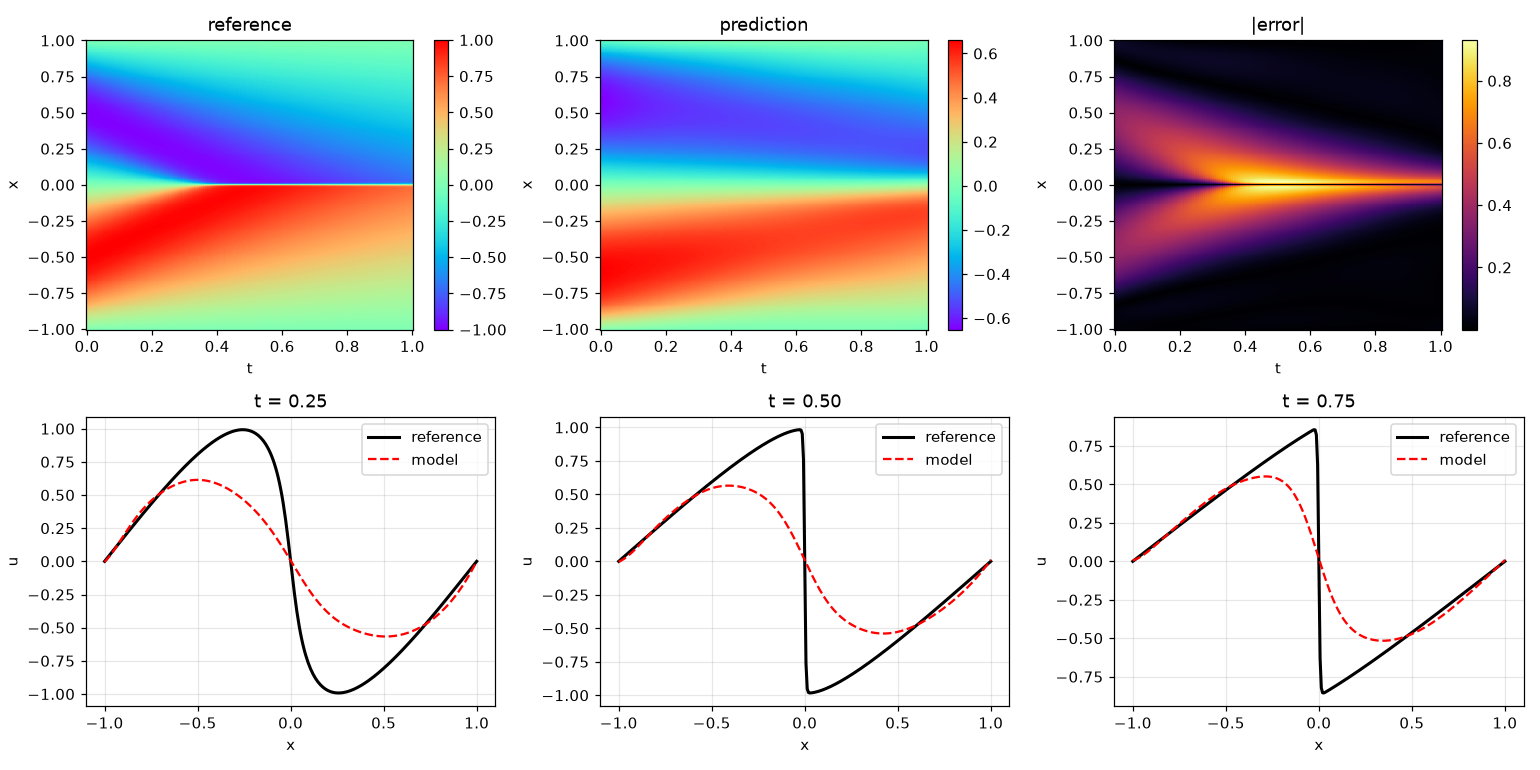
\includegraphics[width=\textwidth]{abl_post_32/figures/solution.png}
\caption{\textbf{abl\_post\_32} --- Predicted field $u(x,t)$ vs.\ exact reference, with the pointwise error map. The shock ($x\!=\!0$) is where a smooth network struggles.}
\end{figure}
\begin{figure}[H]\centering
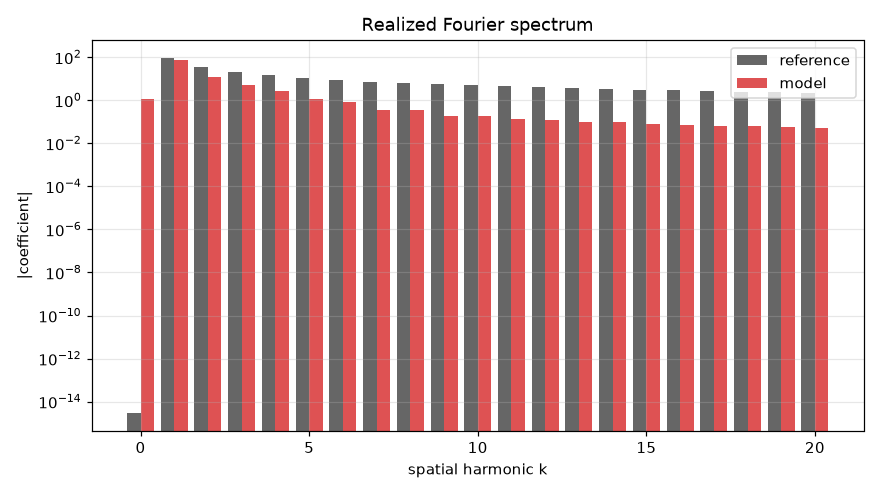
\includegraphics[width=\textwidth]{abl_post_32/figures/spectrum.png}
\caption{\textbf{abl\_post\_32} --- Realized spatial spectrum (per-harmonic magnitude) vs.\ reference. Tests whether the model captures the high-$k$ shock tail or only low frequencies.}
\end{figure}
\begin{figure}[H]\centering
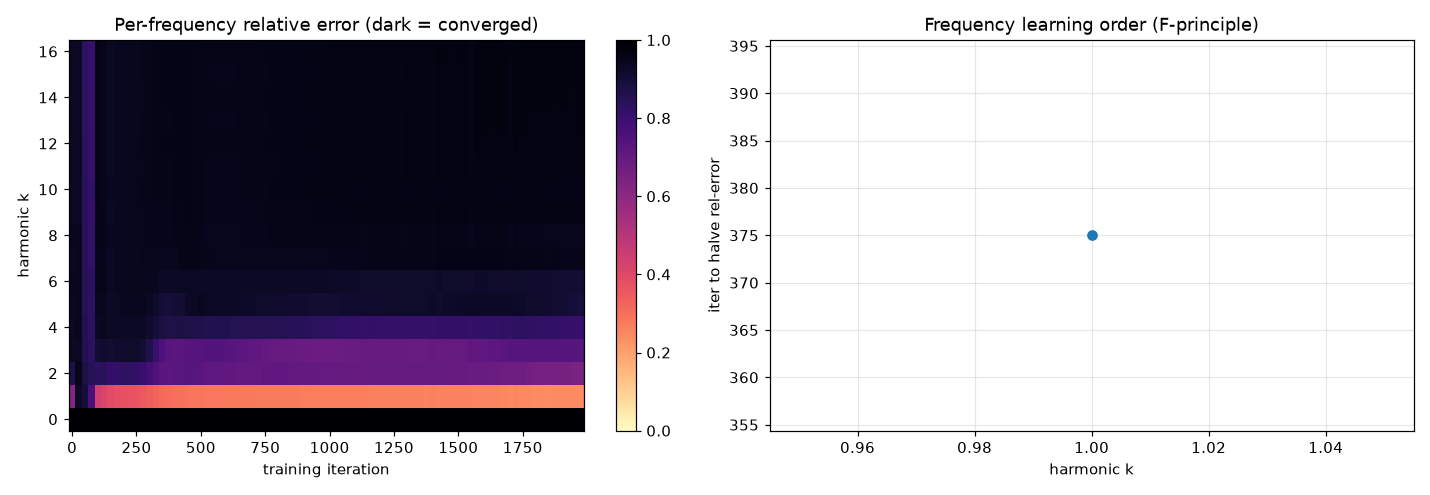
\includegraphics[width=\textwidth]{abl_post_32/figures/fprinciple.png}
\caption{\textbf{abl\_post\_32} --- F-principle heat-map: iteration at which each harmonic's relative error halves. Low harmonics converging first is the F-principle signature.}
\end{figure}
\begin{figure}[H]\centering
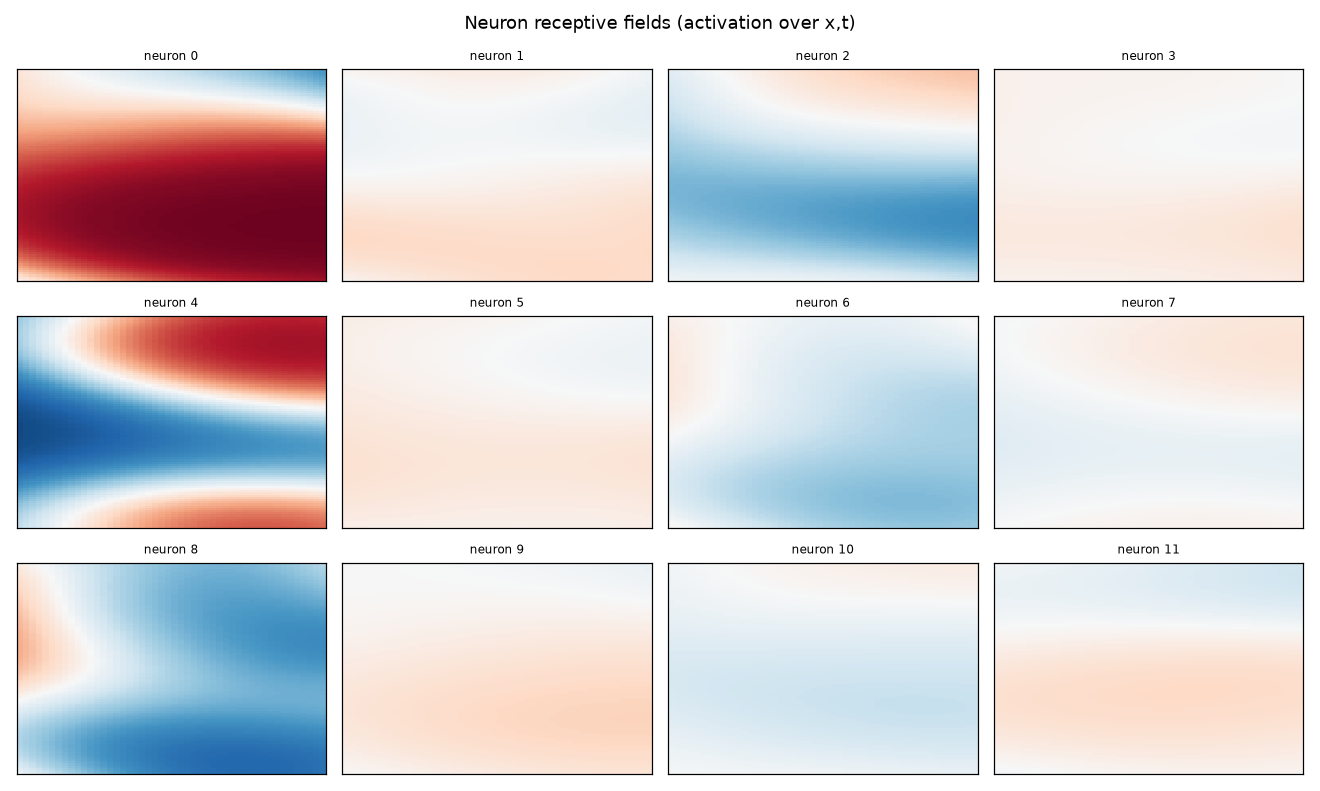
\includegraphics[width=\textwidth]{abl_post_32/figures/neurons.png}
\caption{\textbf{abl\_post\_32} --- Classical post-net neurons: receptive fields over $(x,t)$ and each neuron's dominant spatial frequency / effective rank.}
\end{figure}
\begin{figure}[H]\centering
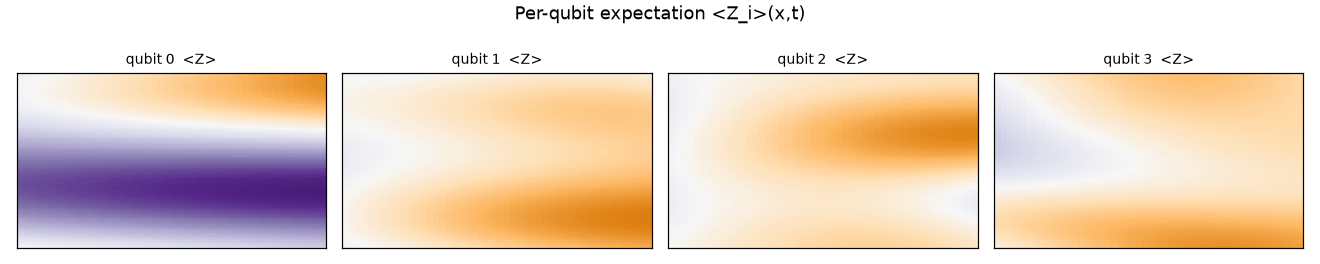
\includegraphics[width=\textwidth]{abl_post_32/figures/qubits.png}
\caption{\textbf{abl\_post\_32} --- Per-qubit $\langle Z\rangle$ receptive fields --- what feature each qubit computes over the domain (quantum models only).}
\end{figure}
\begin{figure}[H]\centering
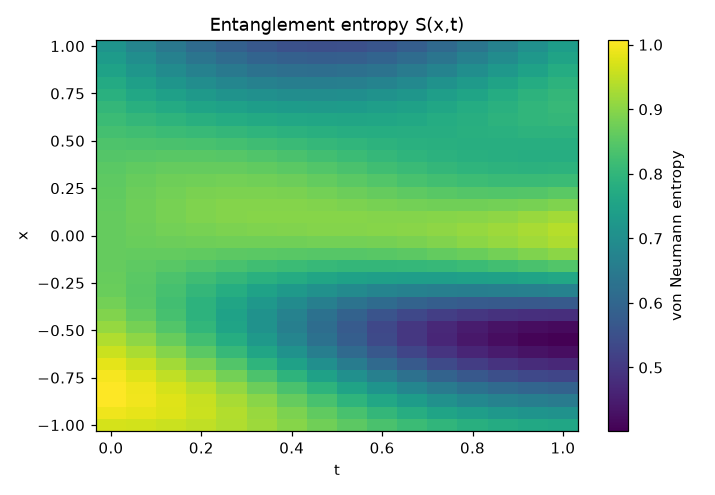
\includegraphics[width=\textwidth]{abl_post_32/figures/entanglement.png}
\caption{\textbf{abl\_post\_32} --- Von Neumann entanglement entropy $S(x,t)$ of a qubit bipartition across the domain (quantum models only).}
\end{figure}
\begin{figure}[H]\centering
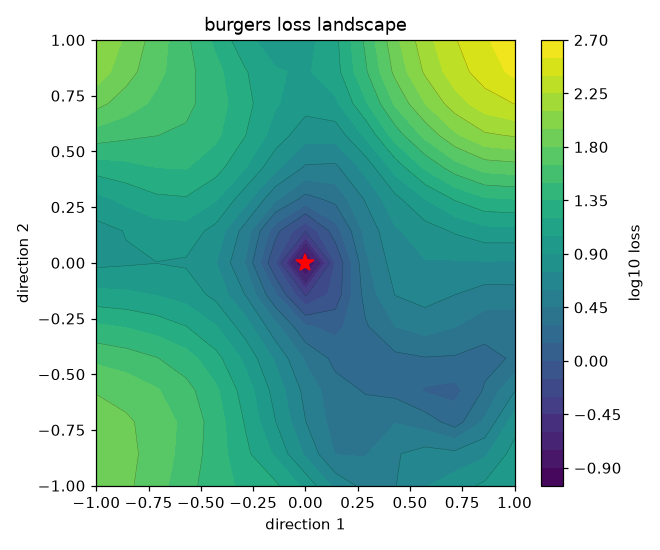
\includegraphics[width=\textwidth]{abl_post_32/figures/landscape.png}
\caption{\textbf{abl\_post\_32} --- Filter-normalized 2-D loss landscape around the trained minimum (Li et al.\ 2018). Flat/wide vs.\ sharp basin.}
\end{figure}
\begin{figure}[H]\centering
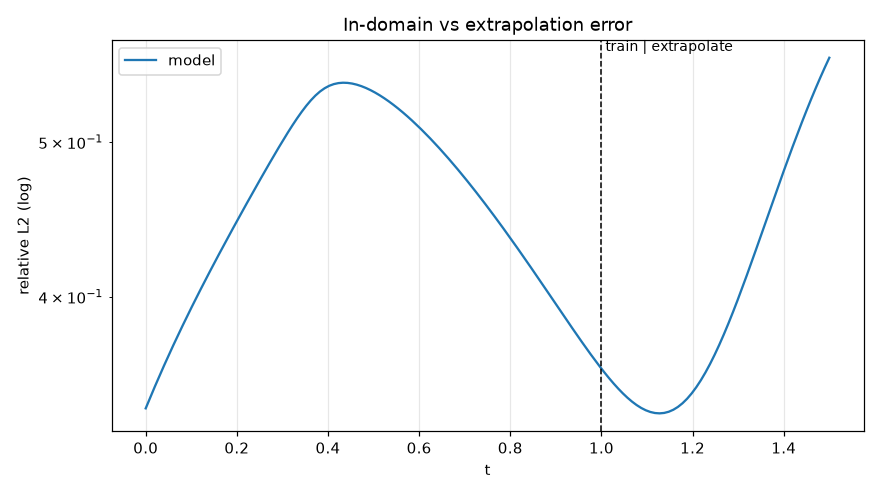
\includegraphics[width=\textwidth]{abl_post_32/figures/generalization.png}
\caption{\textbf{abl\_post\_32} --- Extrapolation: relative $L_2$ vs.\ $t$ beyond the $t\in[0,1]$ training window --- the off-domain penalty.}
\end{figure}
\begin{figure}[H]\centering
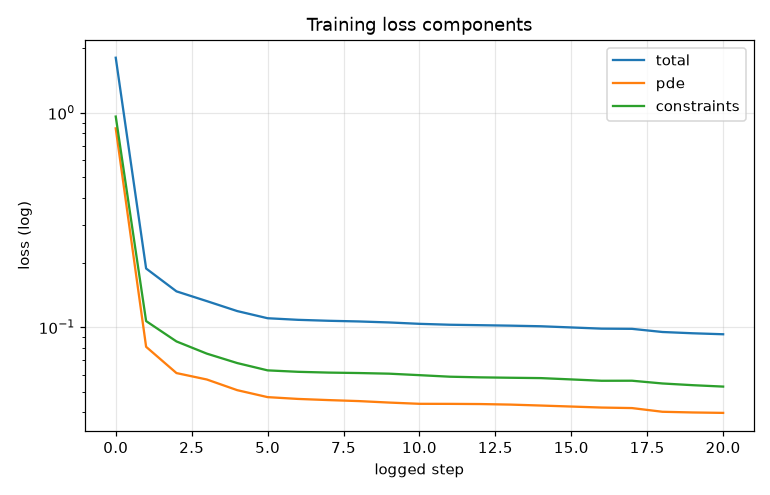
\includegraphics[width=\textwidth]{abl_post_32/figures/loss.png}
\caption{\textbf{abl\_post\_32} --- Training loss history (total, PDE-residual, and constraint terms).}
\end{figure}
\clearpage
\section{Tier-3 ablation --- qubit count}
Another bandwidth knob. Also the axis where a barren-plateau signature appears (gradient variance shrinking with qubits). 4 qubits is the reference run.

\subsection{abl\_qubits\_3}
\noindent\small \textbf{rel-$L_2$}: 0.5011  \textbf{params}: 99  \textbf{PDE}: burgers  \textbf{Adam iters}: 2000  \textbf{seed}: 0  \textbf{model}: qapinn  \textbf{final PDE loss}: 4.42e-02  \textbf{wall time (s)}: 1106  \textbf{VQC}: 3q x3L ent=linear meas=multi scale=1.0\normalsize

\noindent\textbf{Observation.} Prediction colorbar spans about +/-0.6 versus the reference +/-1.0, and the t=0.25/0.50/0.75 snapshots show the red model curve peaking near 0.58 while the black reference reaches 1.0, so the model captures the sinusoidal shape but strongly under-shoots the sawtooth amplitude. The |error| map (colorbar to \textasciitilde{}0.9) is concentrated in a bright fan around the shock at x=0 that widens with t, and the qubits panel shows exactly 3 \textless{}Z\_i\textgreater{} maps; entanglement entropy is low, ranging only \textasciitilde{}0.1 to 0.65 with a dark low-entropy band near x=-0.25. The loss landscape is a clean single convex basin (min log10 loss \textasciitilde{} -0.9 at the red star). Inference: with only 3 qubits the circuit lacks the expressivity/frequency support to resolve the steep shock, so it settles into a smooth amplitude-limited approximation.

\begin{figure}[H]\centering
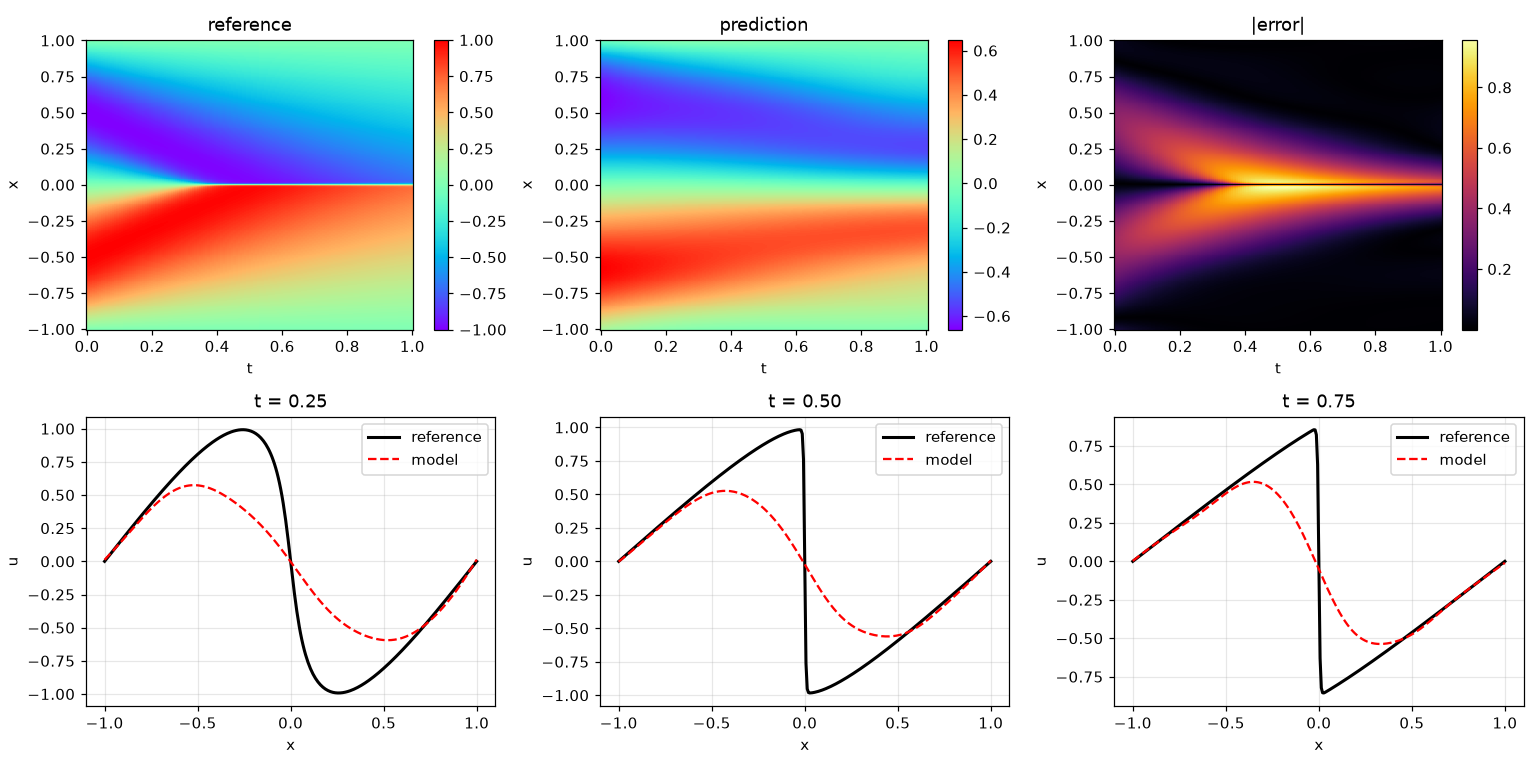
\includegraphics[width=\textwidth]{abl_qubits_3/figures/solution.png}
\caption{\textbf{abl\_qubits\_3} --- Predicted field $u(x,t)$ vs.\ exact reference, with the pointwise error map. The shock ($x\!=\!0$) is where a smooth network struggles.}
\end{figure}
\begin{figure}[H]\centering
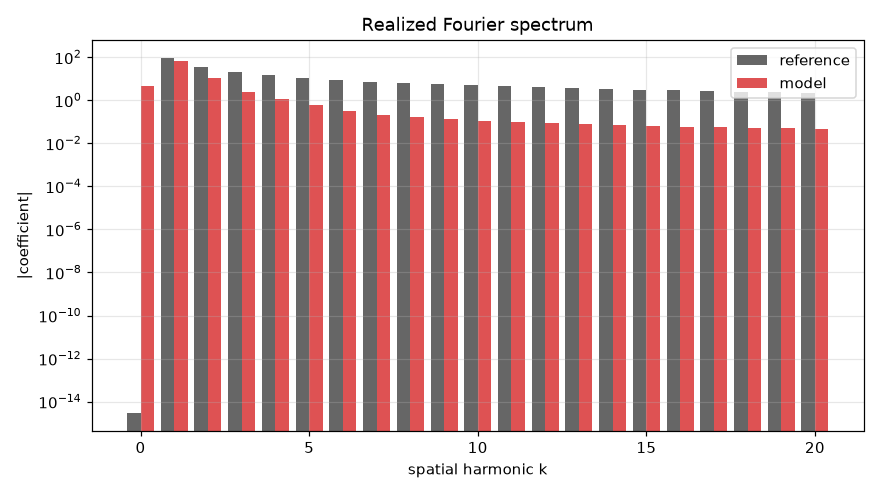
\includegraphics[width=\textwidth]{abl_qubits_3/figures/spectrum.png}
\caption{\textbf{abl\_qubits\_3} --- Realized spatial spectrum (per-harmonic magnitude) vs.\ reference. Tests whether the model captures the high-$k$ shock tail or only low frequencies.}
\end{figure}
\begin{figure}[H]\centering
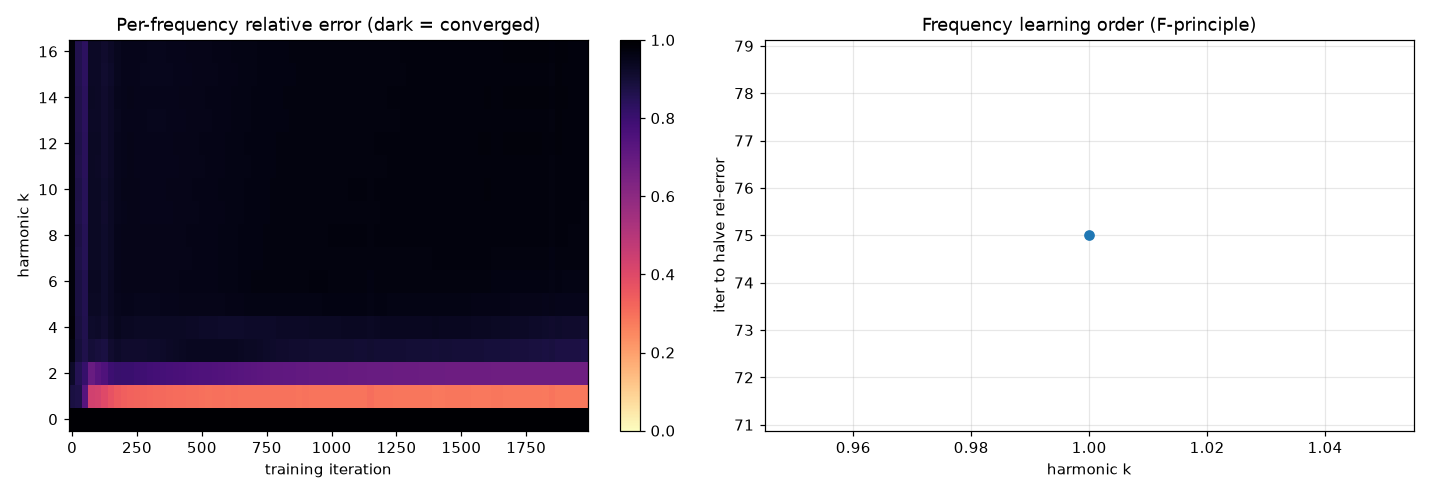
\includegraphics[width=\textwidth]{abl_qubits_3/figures/fprinciple.png}
\caption{\textbf{abl\_qubits\_3} --- F-principle heat-map: iteration at which each harmonic's relative error halves. Low harmonics converging first is the F-principle signature.}
\end{figure}
\begin{figure}[H]\centering
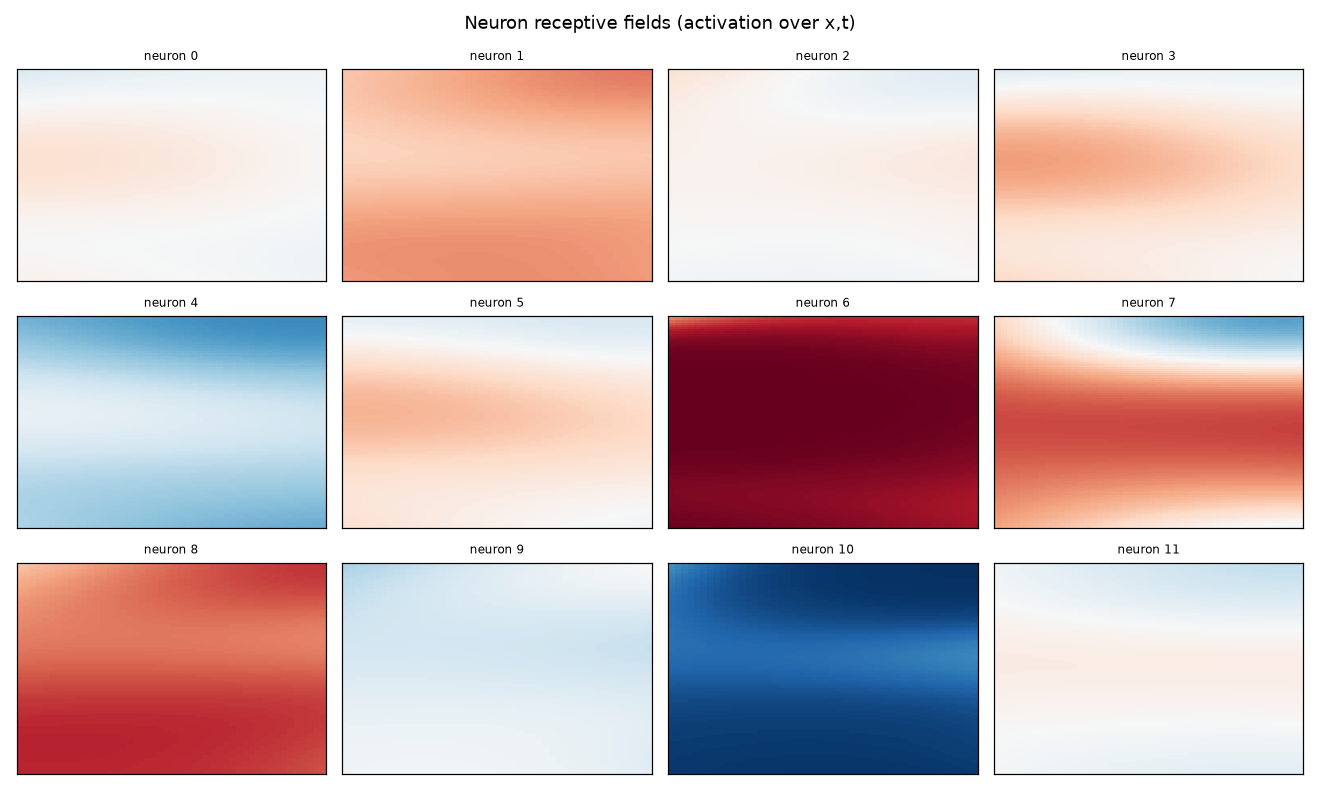
\includegraphics[width=\textwidth]{abl_qubits_3/figures/neurons.png}
\caption{\textbf{abl\_qubits\_3} --- Classical post-net neurons: receptive fields over $(x,t)$ and each neuron's dominant spatial frequency / effective rank.}
\end{figure}
\begin{figure}[H]\centering
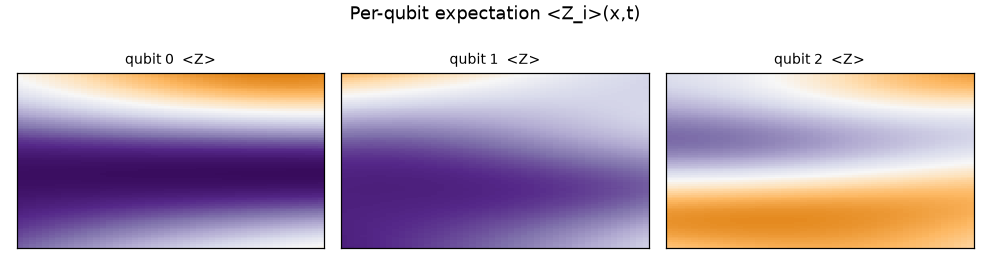
\includegraphics[width=\textwidth]{abl_qubits_3/figures/qubits.png}
\caption{\textbf{abl\_qubits\_3} --- Per-qubit $\langle Z\rangle$ receptive fields --- what feature each qubit computes over the domain (quantum models only).}
\end{figure}
\begin{figure}[H]\centering
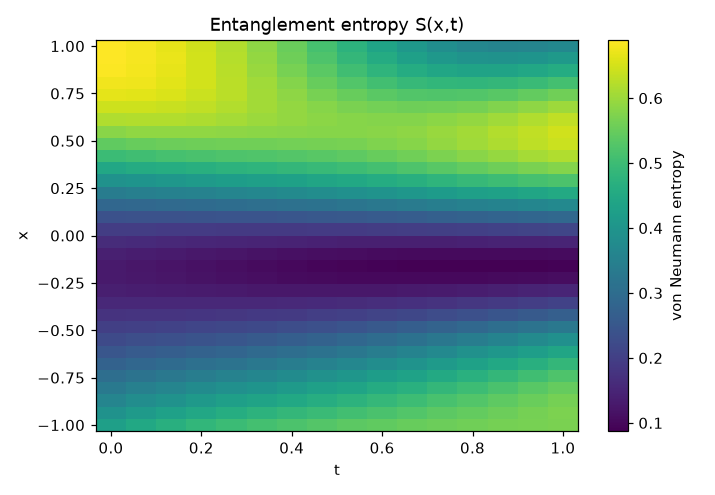
\includegraphics[width=\textwidth]{abl_qubits_3/figures/entanglement.png}
\caption{\textbf{abl\_qubits\_3} --- Von Neumann entanglement entropy $S(x,t)$ of a qubit bipartition across the domain (quantum models only).}
\end{figure}
\begin{figure}[H]\centering
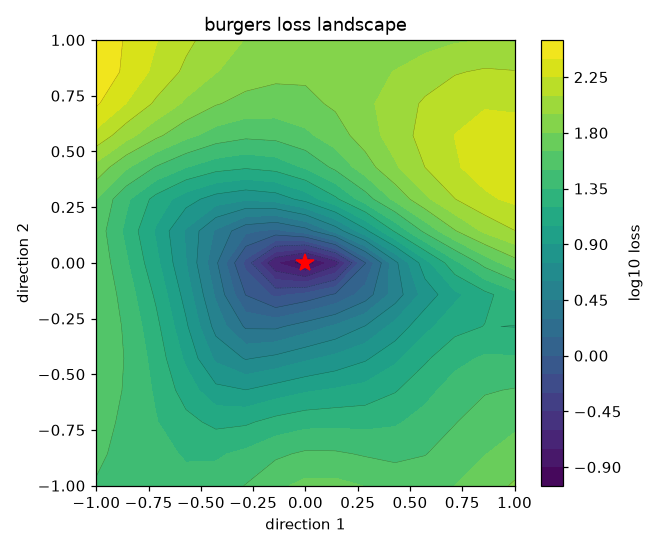
\includegraphics[width=\textwidth]{abl_qubits_3/figures/landscape.png}
\caption{\textbf{abl\_qubits\_3} --- Filter-normalized 2-D loss landscape around the trained minimum (Li et al.\ 2018). Flat/wide vs.\ sharp basin.}
\end{figure}
\begin{figure}[H]\centering
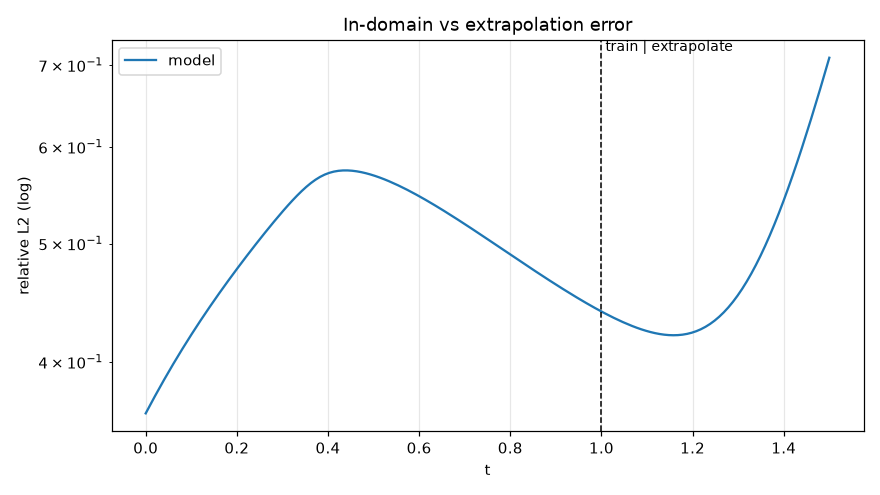
\includegraphics[width=\textwidth]{abl_qubits_3/figures/generalization.png}
\caption{\textbf{abl\_qubits\_3} --- Extrapolation: relative $L_2$ vs.\ $t$ beyond the $t\in[0,1]$ training window --- the off-domain penalty.}
\end{figure}
\begin{figure}[H]\centering
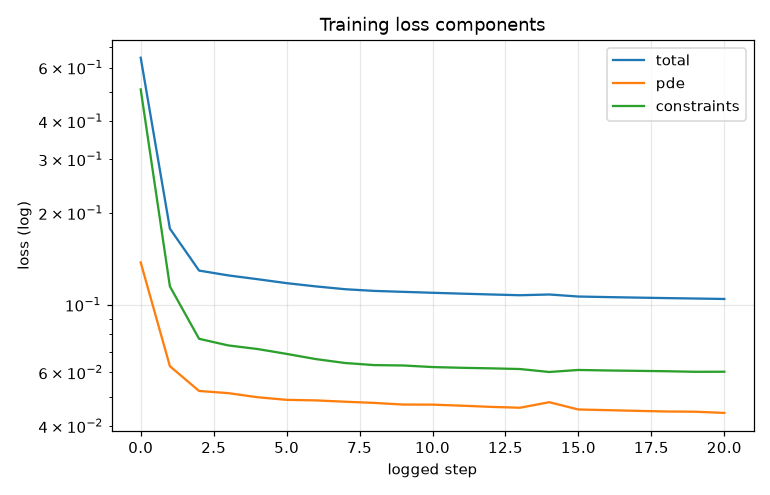
\includegraphics[width=\textwidth]{abl_qubits_3/figures/loss.png}
\caption{\textbf{abl\_qubits\_3} --- Training loss history (total, PDE-residual, and constraint terms).}
\end{figure}
\clearpage
\subsection{abl\_qubits\_5}
\noindent\small \textbf{rel-$L_2$}: 0.4684  \textbf{params}: 143  \textbf{PDE}: burgers  \textbf{Adam iters}: 2000  \textbf{seed}: 0  \textbf{model}: qapinn  \textbf{final PDE loss}: 3.96e-02  \textbf{wall time (s)}: 3651  \textbf{VQC}: 5q x3L ent=linear meas=multi scale=1.0\normalsize

\noindent\textbf{Observation.} Prediction reaches about +/-0.65 and the snapshot model curves peak near 0.60 (still short of the reference 1.0), a modest improvement over the 3-qubit run. The qubits panel now shows 5 \textless{}Z\_i\textgreater{} maps (one full row of 4 plus qubit 4), the error fan at x=0 tops out near 0.9, and entanglement entropy rises to a higher range of \textasciitilde{}0.55 to 1.1 with a low-entropy pocket near (t=0.3, x=-0.3). The generalization curve dips to its minimum (\textasciitilde{}0.42 relative L2) just past the train|extrapolate line at t\textasciitilde{}1.1 before rising to \textasciitilde{}0.65 by t=1.5. Inference: adding qubits increases available entanglement and slightly improves amplitude recovery, confirming a mild capacity benefit without fully resolving the shock.

\begin{figure}[H]\centering
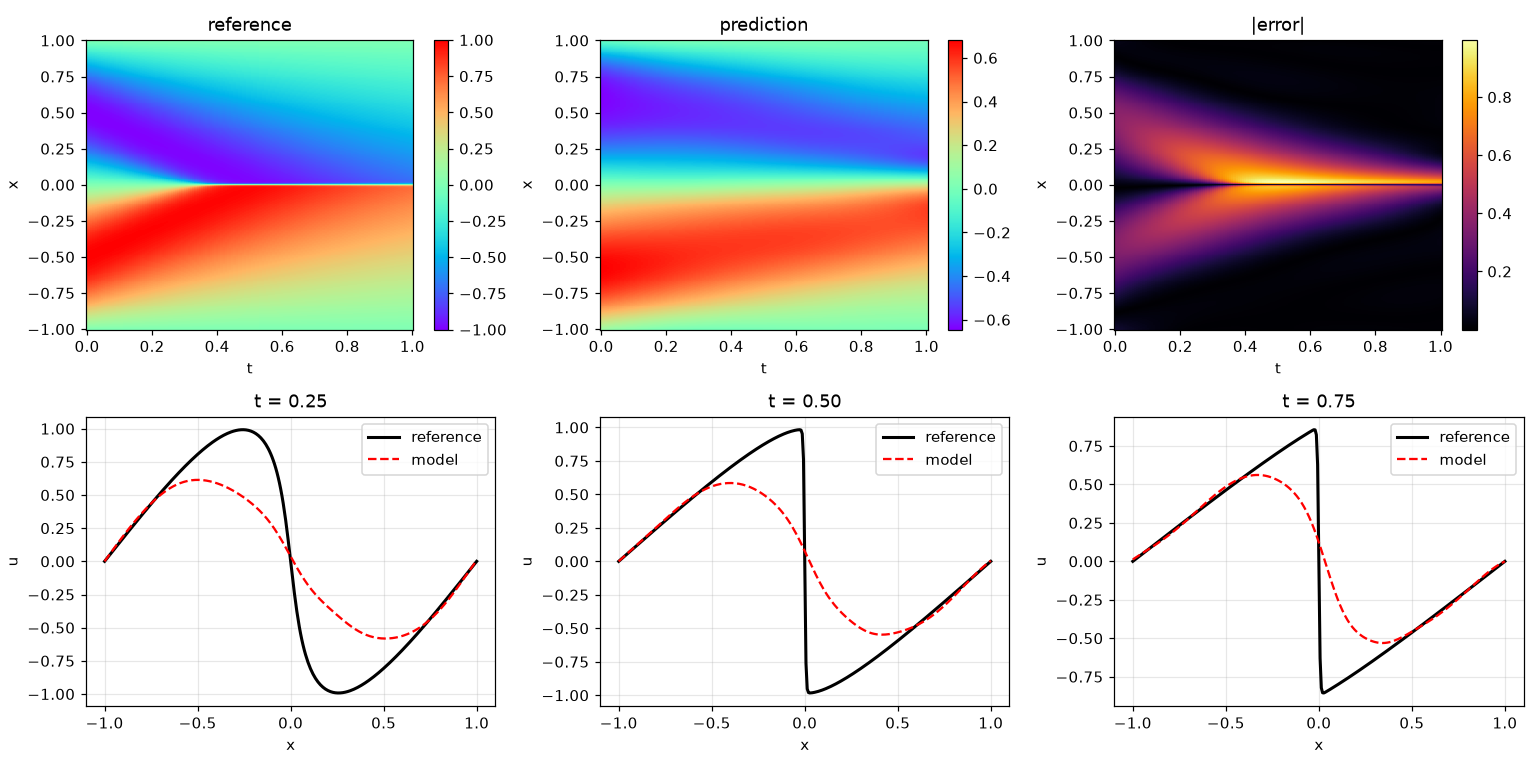
\includegraphics[width=\textwidth]{abl_qubits_5/figures/solution.png}
\caption{\textbf{abl\_qubits\_5} --- Predicted field $u(x,t)$ vs.\ exact reference, with the pointwise error map. The shock ($x\!=\!0$) is where a smooth network struggles.}
\end{figure}
\begin{figure}[H]\centering
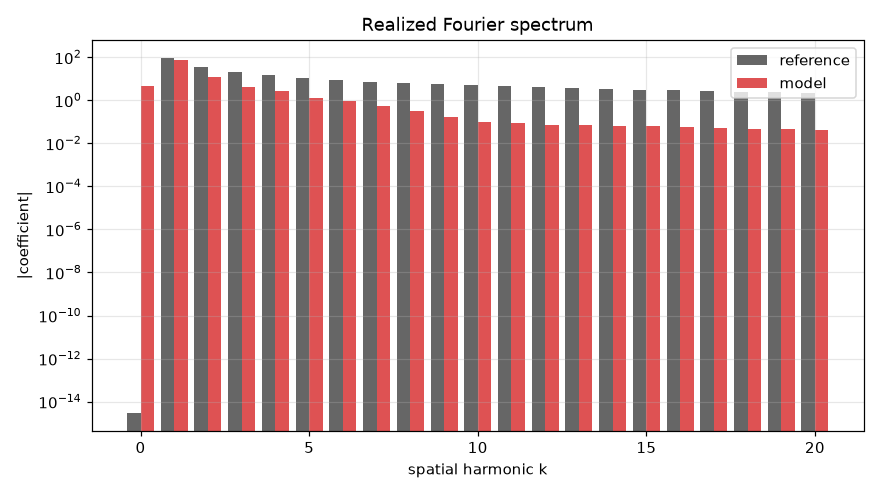
\includegraphics[width=\textwidth]{abl_qubits_5/figures/spectrum.png}
\caption{\textbf{abl\_qubits\_5} --- Realized spatial spectrum (per-harmonic magnitude) vs.\ reference. Tests whether the model captures the high-$k$ shock tail or only low frequencies.}
\end{figure}
\begin{figure}[H]\centering
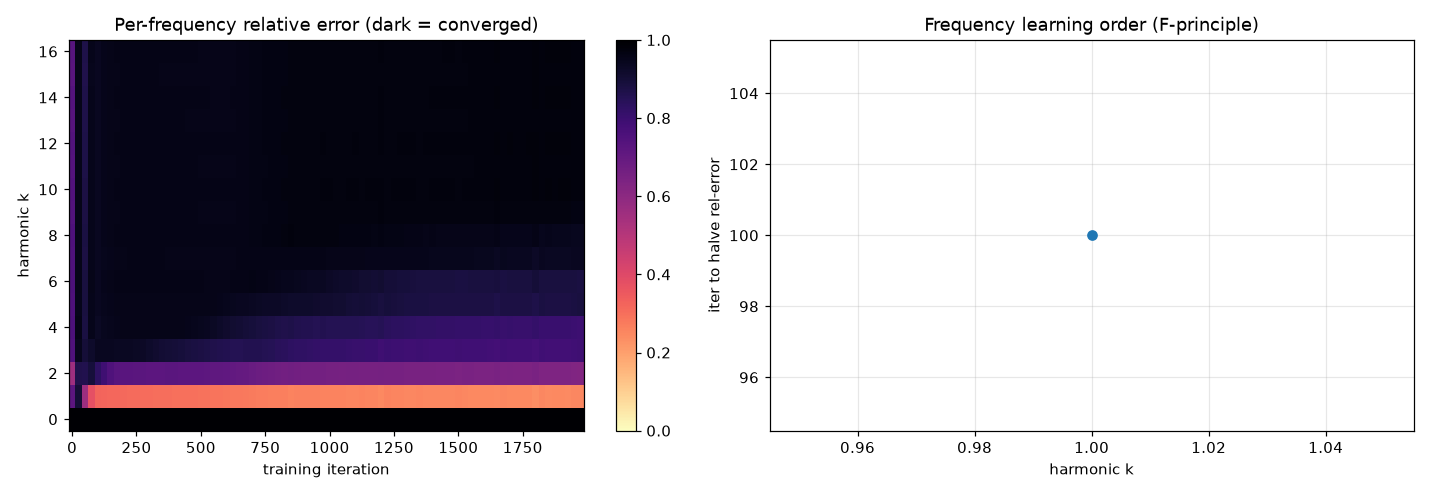
\includegraphics[width=\textwidth]{abl_qubits_5/figures/fprinciple.png}
\caption{\textbf{abl\_qubits\_5} --- F-principle heat-map: iteration at which each harmonic's relative error halves. Low harmonics converging first is the F-principle signature.}
\end{figure}
\begin{figure}[H]\centering
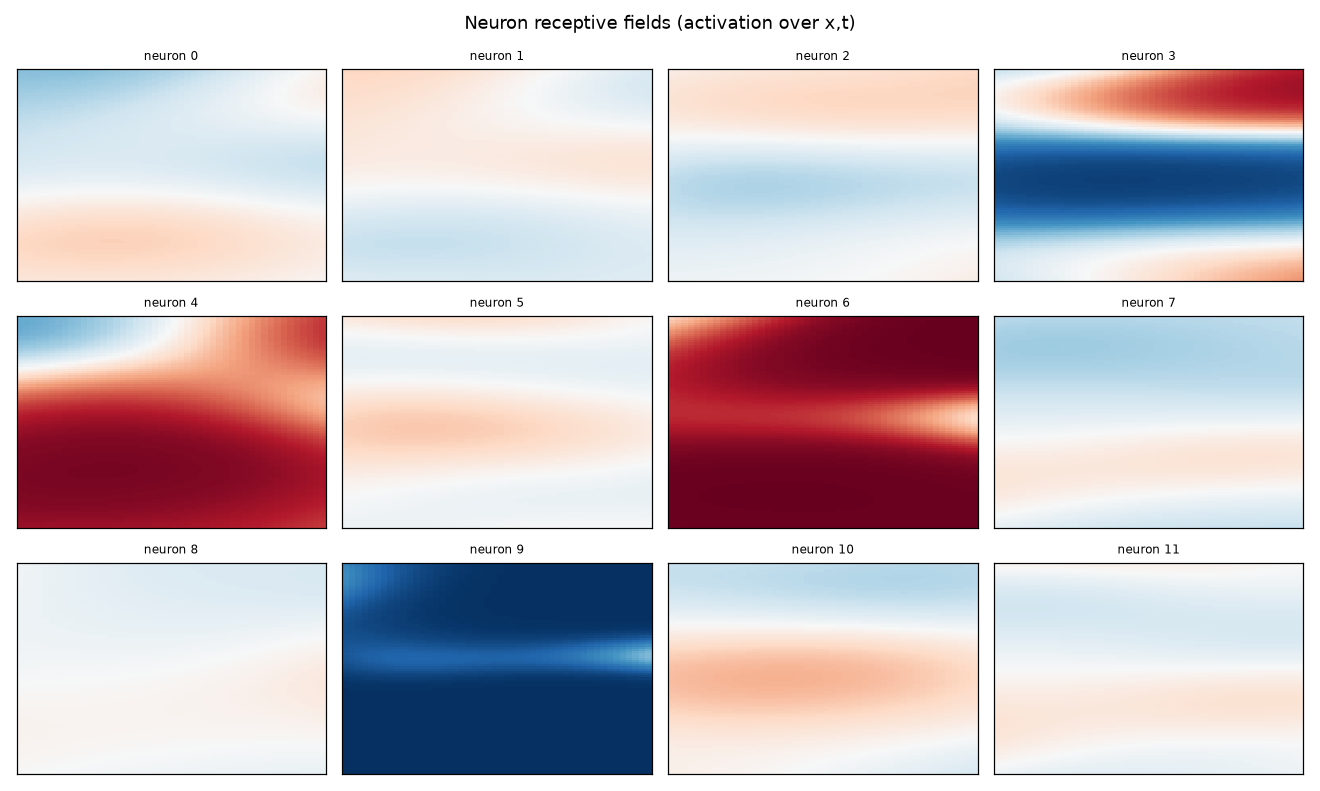
\includegraphics[width=\textwidth]{abl_qubits_5/figures/neurons.png}
\caption{\textbf{abl\_qubits\_5} --- Classical post-net neurons: receptive fields over $(x,t)$ and each neuron's dominant spatial frequency / effective rank.}
\end{figure}
\begin{figure}[H]\centering
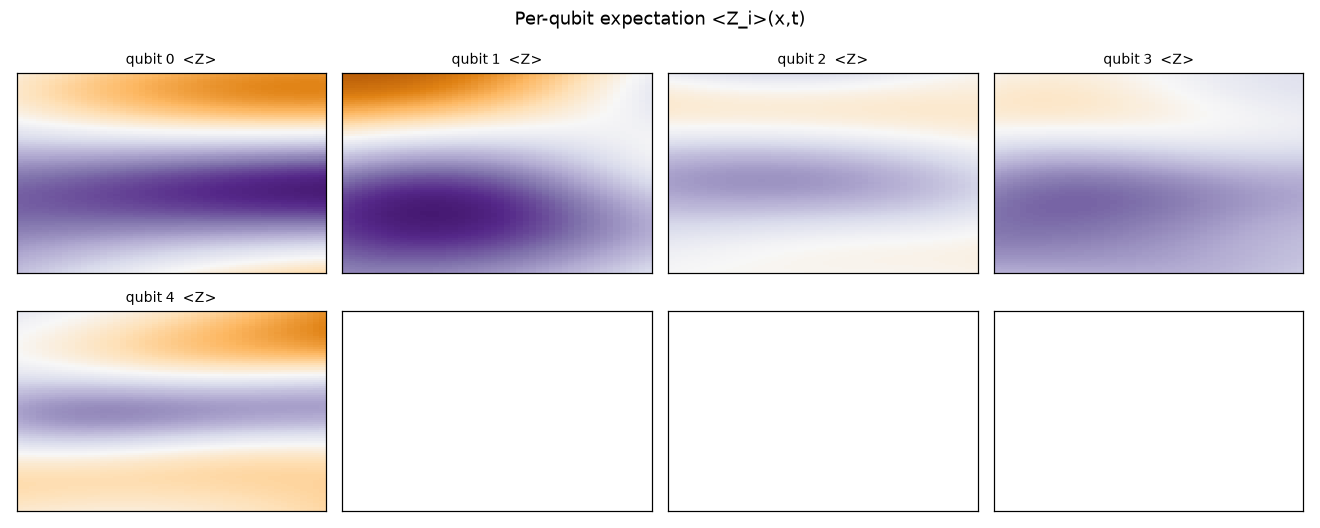
\includegraphics[width=\textwidth]{abl_qubits_5/figures/qubits.png}
\caption{\textbf{abl\_qubits\_5} --- Per-qubit $\langle Z\rangle$ receptive fields --- what feature each qubit computes over the domain (quantum models only).}
\end{figure}
\begin{figure}[H]\centering
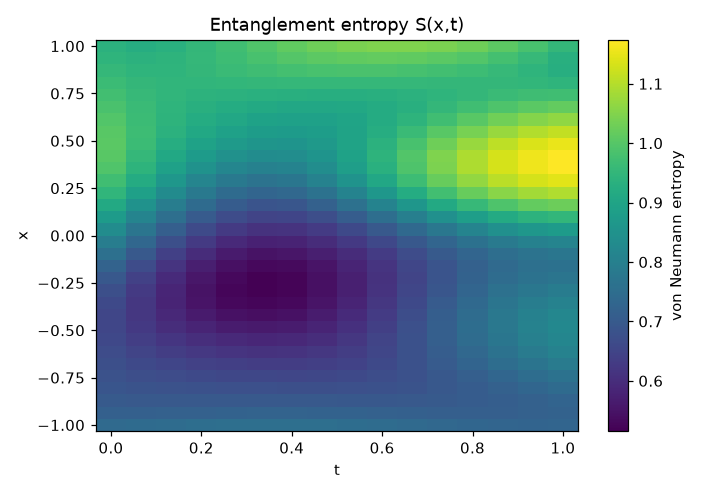
\includegraphics[width=\textwidth]{abl_qubits_5/figures/entanglement.png}
\caption{\textbf{abl\_qubits\_5} --- Von Neumann entanglement entropy $S(x,t)$ of a qubit bipartition across the domain (quantum models only).}
\end{figure}
\begin{figure}[H]\centering
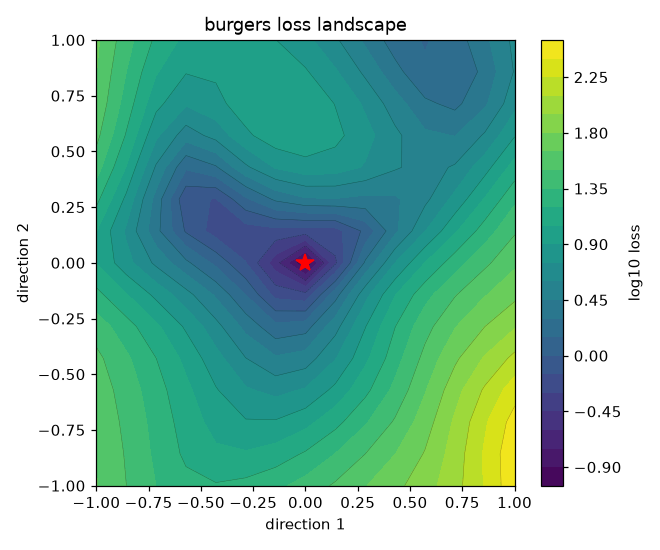
\includegraphics[width=\textwidth]{abl_qubits_5/figures/landscape.png}
\caption{\textbf{abl\_qubits\_5} --- Filter-normalized 2-D loss landscape around the trained minimum (Li et al.\ 2018). Flat/wide vs.\ sharp basin.}
\end{figure}
\begin{figure}[H]\centering
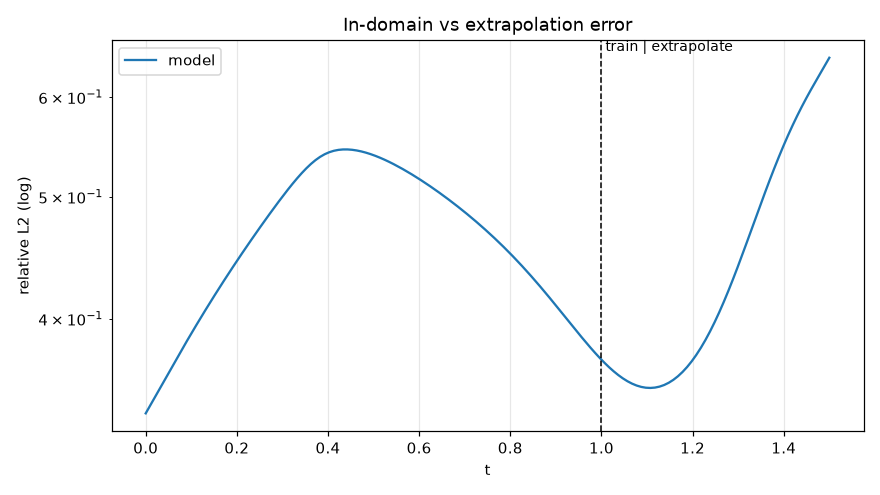
\includegraphics[width=\textwidth]{abl_qubits_5/figures/generalization.png}
\caption{\textbf{abl\_qubits\_5} --- Extrapolation: relative $L_2$ vs.\ $t$ beyond the $t\in[0,1]$ training window --- the off-domain penalty.}
\end{figure}
\begin{figure}[H]\centering
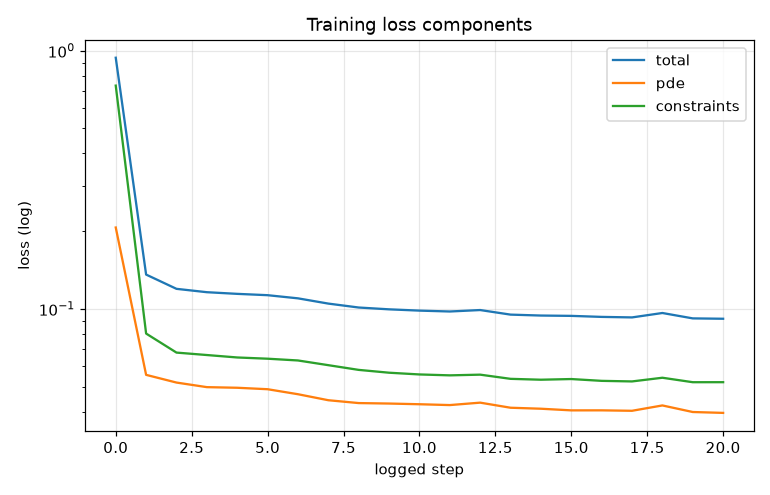
\includegraphics[width=\textwidth]{abl_qubits_5/figures/loss.png}
\caption{\textbf{abl\_qubits\_5} --- Training loss history (total, PDE-residual, and constraint terms).}
\end{figure}
\clearpage
\subsection{abl\_qubits\_6}
\noindent\small \textbf{rel-$L_2$}: 0.4429  \textbf{params}: 165  \textbf{PDE}: burgers  \textbf{Adam iters}: 2000  \textbf{seed}: 0  \textbf{model}: qapinn  \textbf{final PDE loss}: 3.71e-02  \textbf{wall time (s)}: 4691  \textbf{VQC}: 6q x3L ent=linear meas=multi scale=1.0\normalsize

\noindent\textbf{Observation.} Prediction spans roughly +/-0.6 to 0.65 with snapshot peaks near 0.6, comparable to the 5-qubit case, and the |error| colorbar now reaches the full 1.0 in the shock fan at x=0. The qubits panel displays 6 \textless{}Z\_i\textgreater{} maps (4+2), and entanglement entropy is the highest of the qubit sweep, ranging \textasciitilde{}0.65 up to \textasciitilde{}1.35 with a dark low-entropy blob near (t=0.15, x=0.2). The Fourier spectrum tracks the reference through k\textasciitilde{}3 then the model bars fall increasingly below reference for k\textgreater{}4. Inference: entanglement scales monotonically with qubit count (3-\textgreater{}\textasciitilde{}0.65, 5-\textgreater{}\textasciitilde{}1.1, 6-\textgreater{}\textasciitilde{}1.35) yet reconstruction accuracy saturates, indicating diminishing returns beyond \textasciitilde{}5 qubits for this Burgers problem.

\begin{figure}[H]\centering
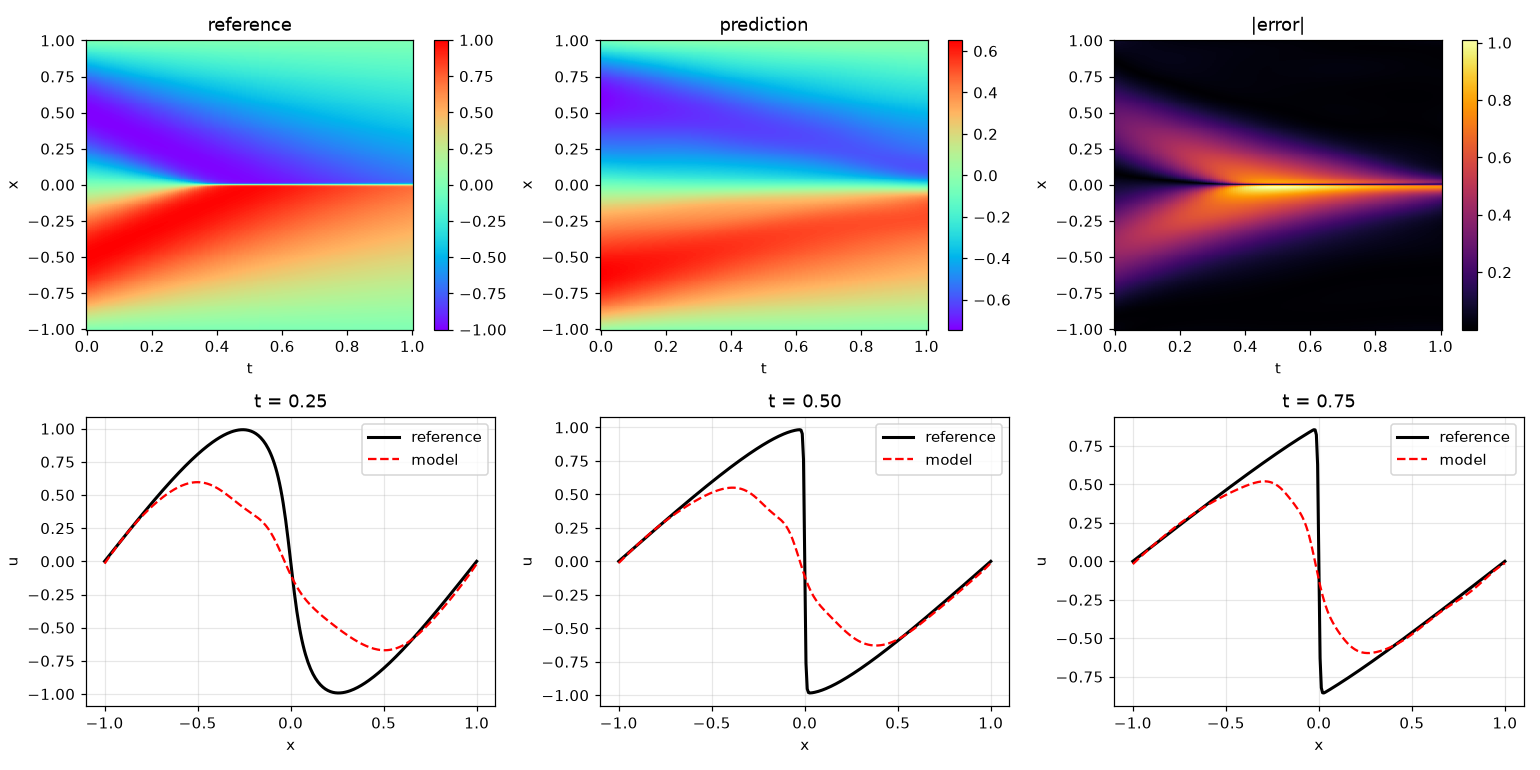
\includegraphics[width=\textwidth]{abl_qubits_6/figures/solution.png}
\caption{\textbf{abl\_qubits\_6} --- Predicted field $u(x,t)$ vs.\ exact reference, with the pointwise error map. The shock ($x\!=\!0$) is where a smooth network struggles.}
\end{figure}
\begin{figure}[H]\centering
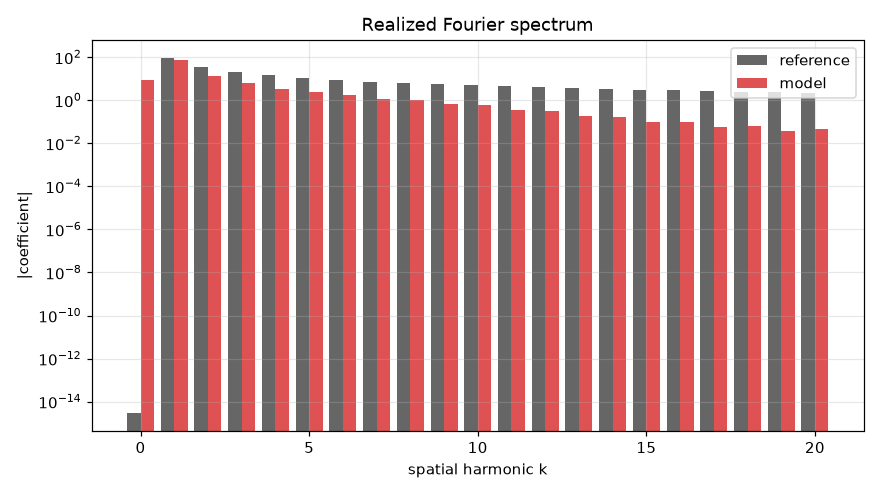
\includegraphics[width=\textwidth]{abl_qubits_6/figures/spectrum.png}
\caption{\textbf{abl\_qubits\_6} --- Realized spatial spectrum (per-harmonic magnitude) vs.\ reference. Tests whether the model captures the high-$k$ shock tail or only low frequencies.}
\end{figure}
\begin{figure}[H]\centering
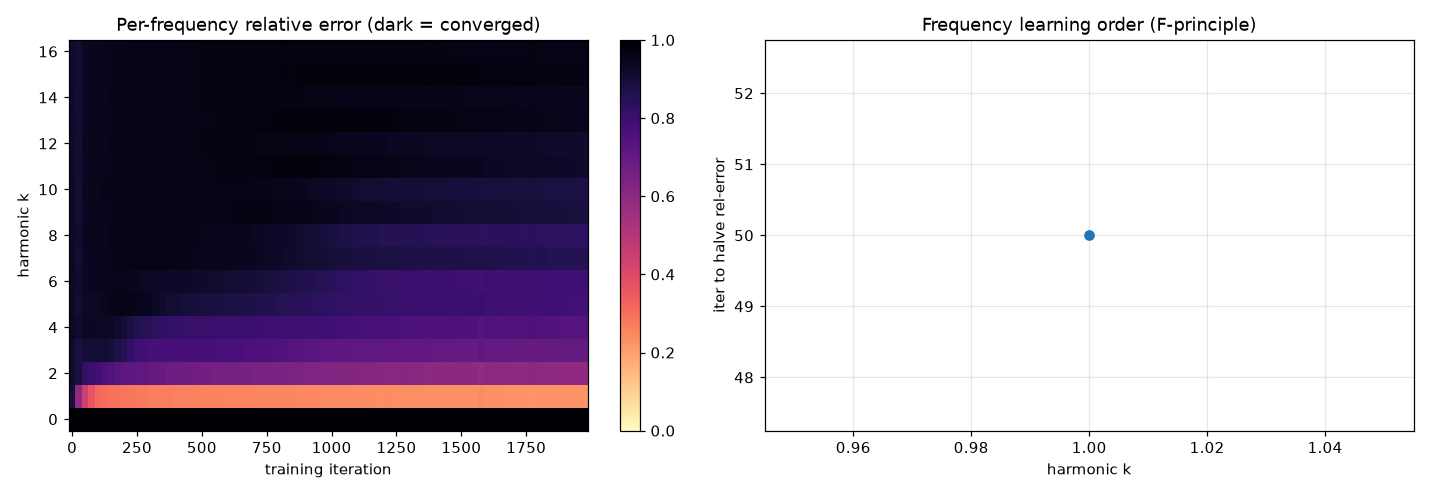
\includegraphics[width=\textwidth]{abl_qubits_6/figures/fprinciple.png}
\caption{\textbf{abl\_qubits\_6} --- F-principle heat-map: iteration at which each harmonic's relative error halves. Low harmonics converging first is the F-principle signature.}
\end{figure}
\begin{figure}[H]\centering
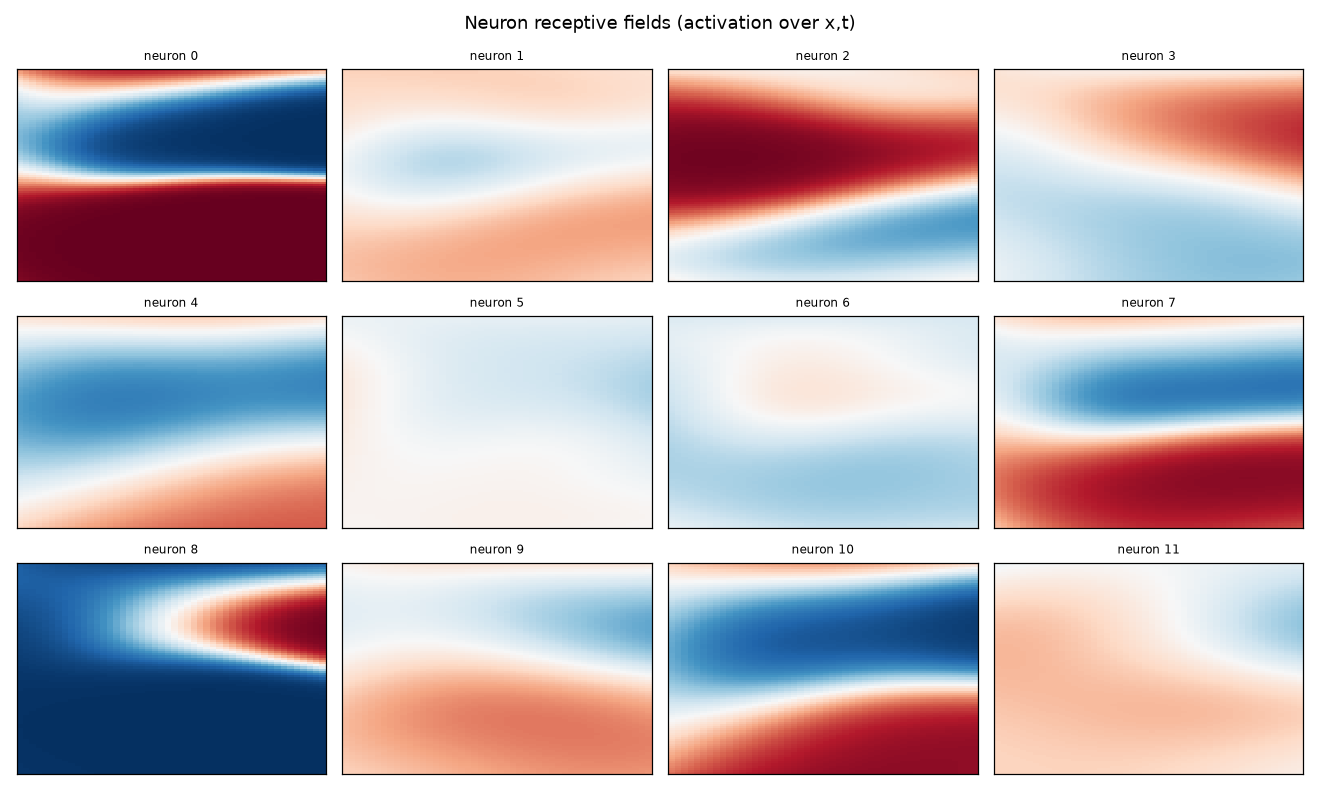
\includegraphics[width=\textwidth]{abl_qubits_6/figures/neurons.png}
\caption{\textbf{abl\_qubits\_6} --- Classical post-net neurons: receptive fields over $(x,t)$ and each neuron's dominant spatial frequency / effective rank.}
\end{figure}
\begin{figure}[H]\centering
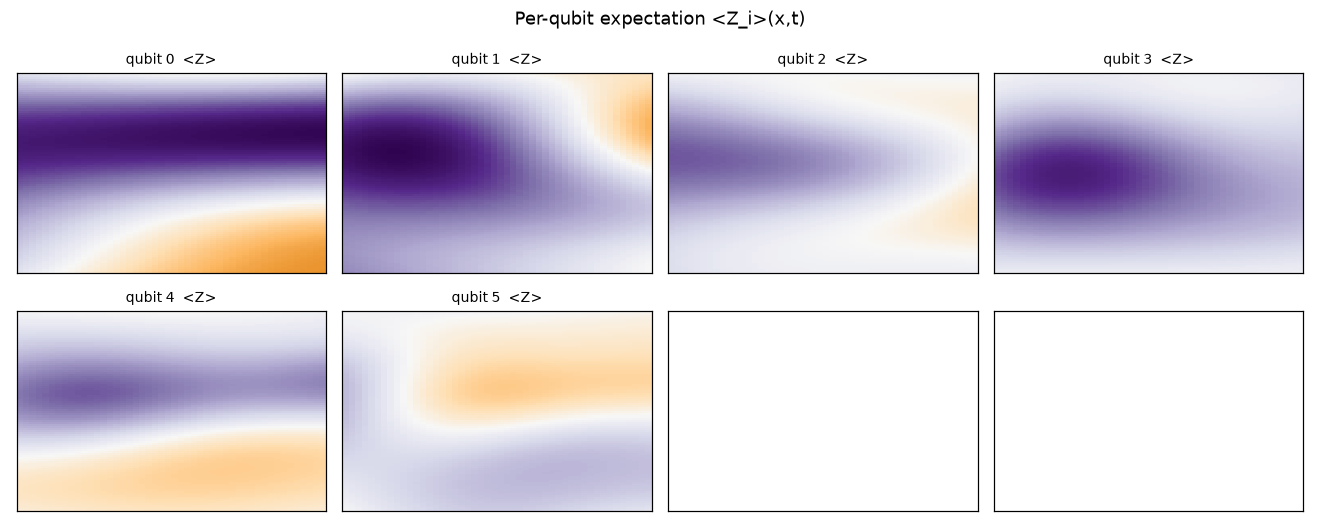
\includegraphics[width=\textwidth]{abl_qubits_6/figures/qubits.png}
\caption{\textbf{abl\_qubits\_6} --- Per-qubit $\langle Z\rangle$ receptive fields --- what feature each qubit computes over the domain (quantum models only).}
\end{figure}
\begin{figure}[H]\centering
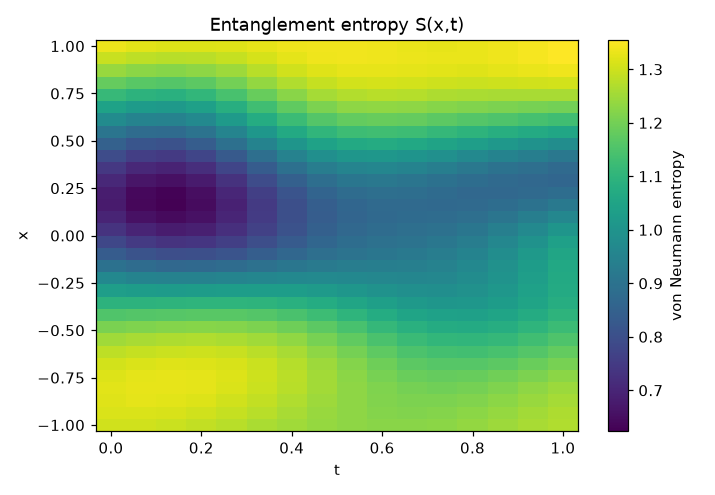
\includegraphics[width=\textwidth]{abl_qubits_6/figures/entanglement.png}
\caption{\textbf{abl\_qubits\_6} --- Von Neumann entanglement entropy $S(x,t)$ of a qubit bipartition across the domain (quantum models only).}
\end{figure}
\begin{figure}[H]\centering
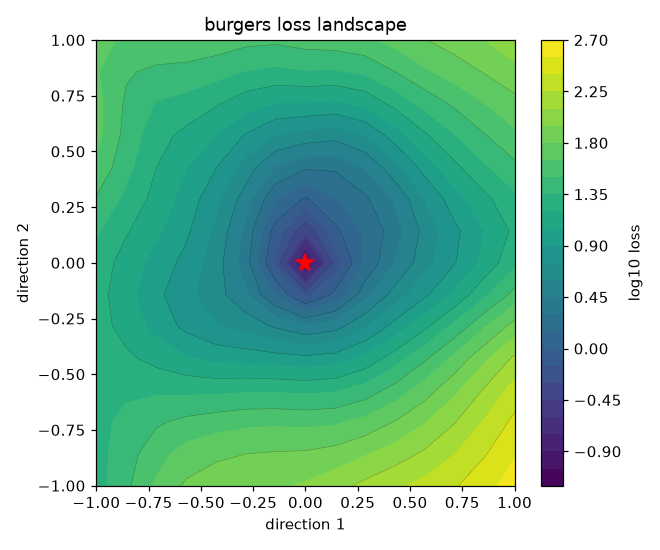
\includegraphics[width=\textwidth]{abl_qubits_6/figures/landscape.png}
\caption{\textbf{abl\_qubits\_6} --- Filter-normalized 2-D loss landscape around the trained minimum (Li et al.\ 2018). Flat/wide vs.\ sharp basin.}
\end{figure}
\begin{figure}[H]\centering
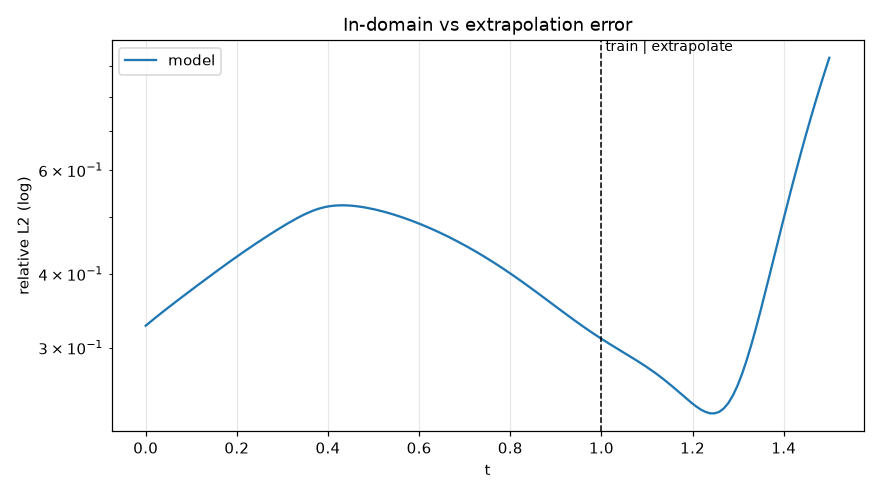
\includegraphics[width=\textwidth]{abl_qubits_6/figures/generalization.png}
\caption{\textbf{abl\_qubits\_6} --- Extrapolation: relative $L_2$ vs.\ $t$ beyond the $t\in[0,1]$ training window --- the off-domain penalty.}
\end{figure}
\begin{figure}[H]\centering
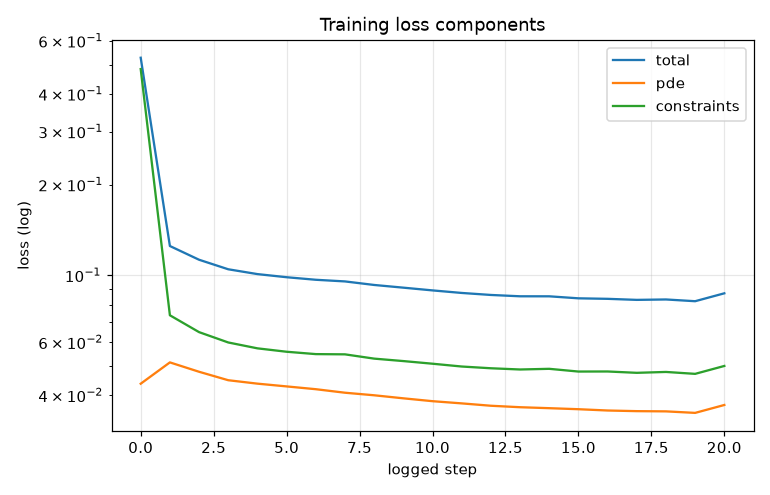
\includegraphics[width=\textwidth]{abl_qubits_6/figures/loss.png}
\caption{\textbf{abl\_qubits\_6} --- Training loss history (total, PDE-residual, and constraint terms).}
\end{figure}
\clearpage
\section{Tier-3 ablation --- measurement operator}
Readout width and correlator type: single-$Z$ vs.\ multi-$Z$ (reference) vs.\ $ZZ$.

\subsection{abl\_meas\_single}
\noindent\small \textbf{rel-$L_2$}: 0.5911  \textbf{params}: 73  \textbf{PDE}: burgers  \textbf{Adam iters}: 2000  \textbf{seed}: 0  \textbf{model}: qapinn  \textbf{final PDE loss}: 5.90e-02  \textbf{wall time (s)}: 1614  \textbf{VQC}: 4q x3L ent=linear meas=single scale=1.0\normalsize

\noindent\textbf{Observation.} Single-Z readout gives the weakest amplitude of the measurement variants: the prediction colorbar is only +/-0.5 and snapshot model peaks reach \textasciitilde{}0.47 versus reference 1.0. The error fan around x=0 brightens to \textasciitilde{}0.9, the qubits panel shows 4 \textless{}Z\_i\textgreater{} maps, and entanglement entropy runs \textasciitilde{}0.68 to 1.05 with a bright high-entropy band in the upper half (x\textgreater{}0.5) and dark pockets at the corners. The realized spectrum matches reference at k=1 but model harmonics for k\textgreater{}=4 sit \textasciitilde{}1 order below reference. Inference: restricting the observable to a single-qubit Z expectation limits the expressible output range, producing the smallest-amplitude fit and confirming the readout choice caps reconstruction fidelity.

\begin{figure}[H]\centering
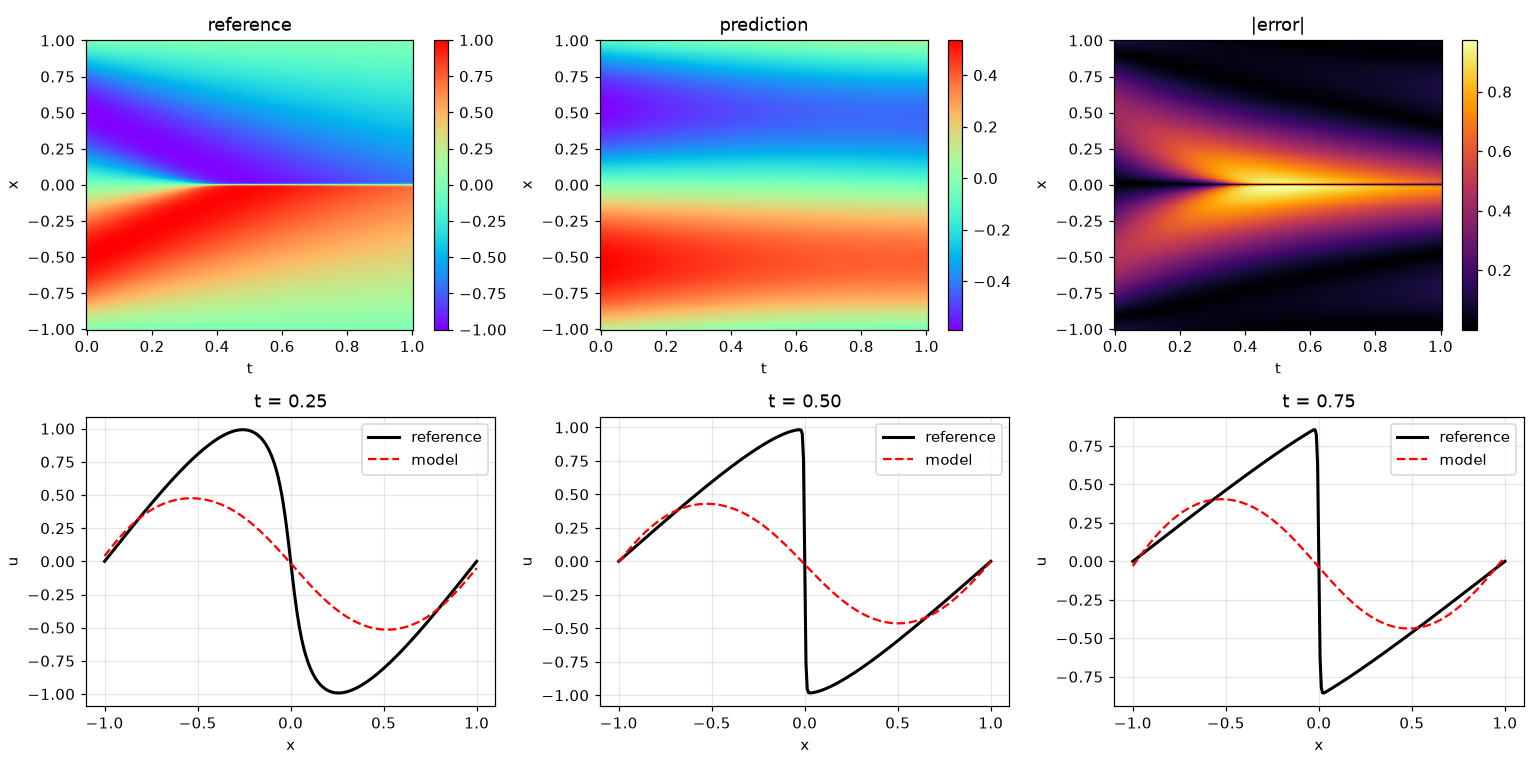
\includegraphics[width=\textwidth]{abl_meas_single/figures/solution.png}
\caption{\textbf{abl\_meas\_single} --- Predicted field $u(x,t)$ vs.\ exact reference, with the pointwise error map. The shock ($x\!=\!0$) is where a smooth network struggles.}
\end{figure}
\begin{figure}[H]\centering
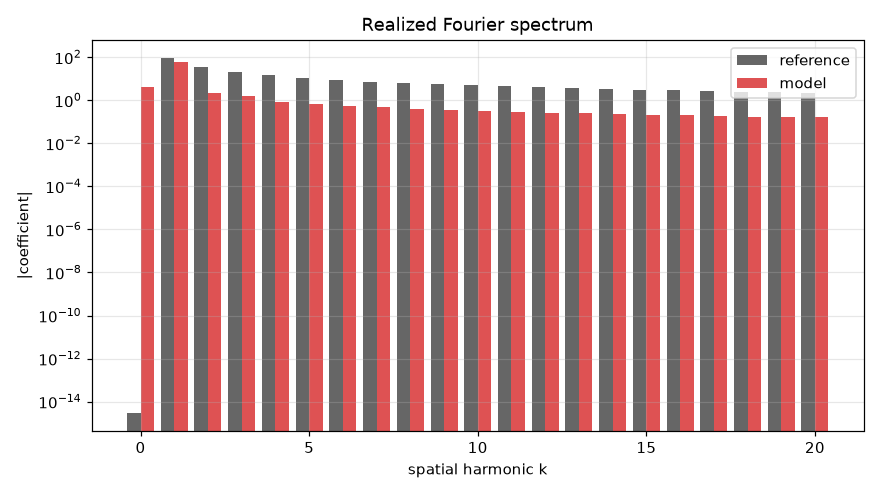
\includegraphics[width=\textwidth]{abl_meas_single/figures/spectrum.png}
\caption{\textbf{abl\_meas\_single} --- Realized spatial spectrum (per-harmonic magnitude) vs.\ reference. Tests whether the model captures the high-$k$ shock tail or only low frequencies.}
\end{figure}
\begin{figure}[H]\centering
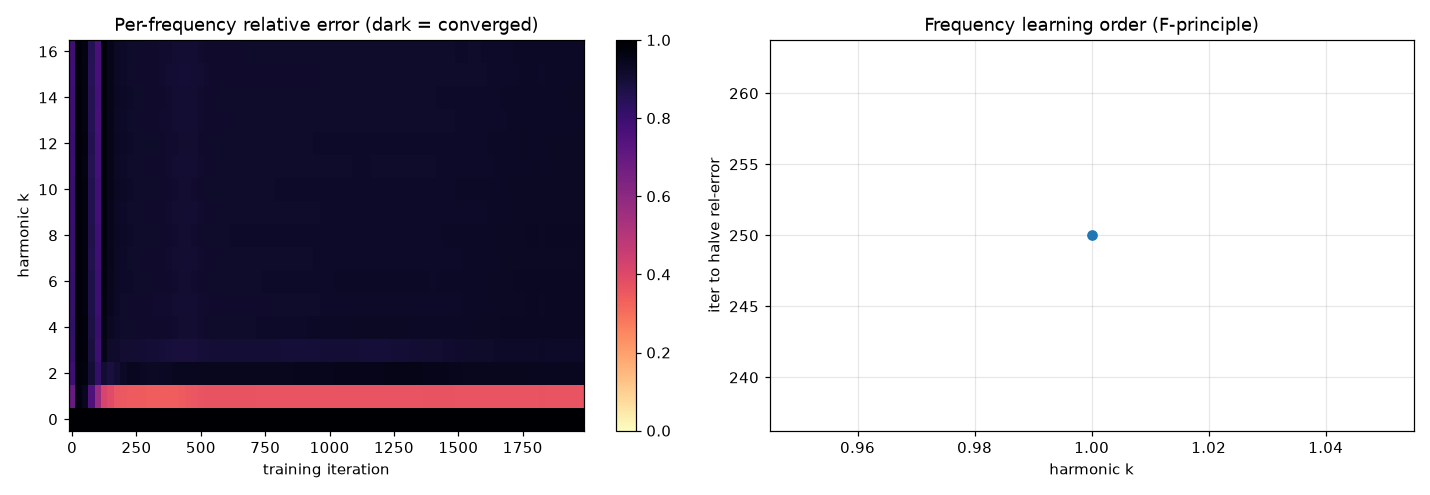
\includegraphics[width=\textwidth]{abl_meas_single/figures/fprinciple.png}
\caption{\textbf{abl\_meas\_single} --- F-principle heat-map: iteration at which each harmonic's relative error halves. Low harmonics converging first is the F-principle signature.}
\end{figure}
\begin{figure}[H]\centering
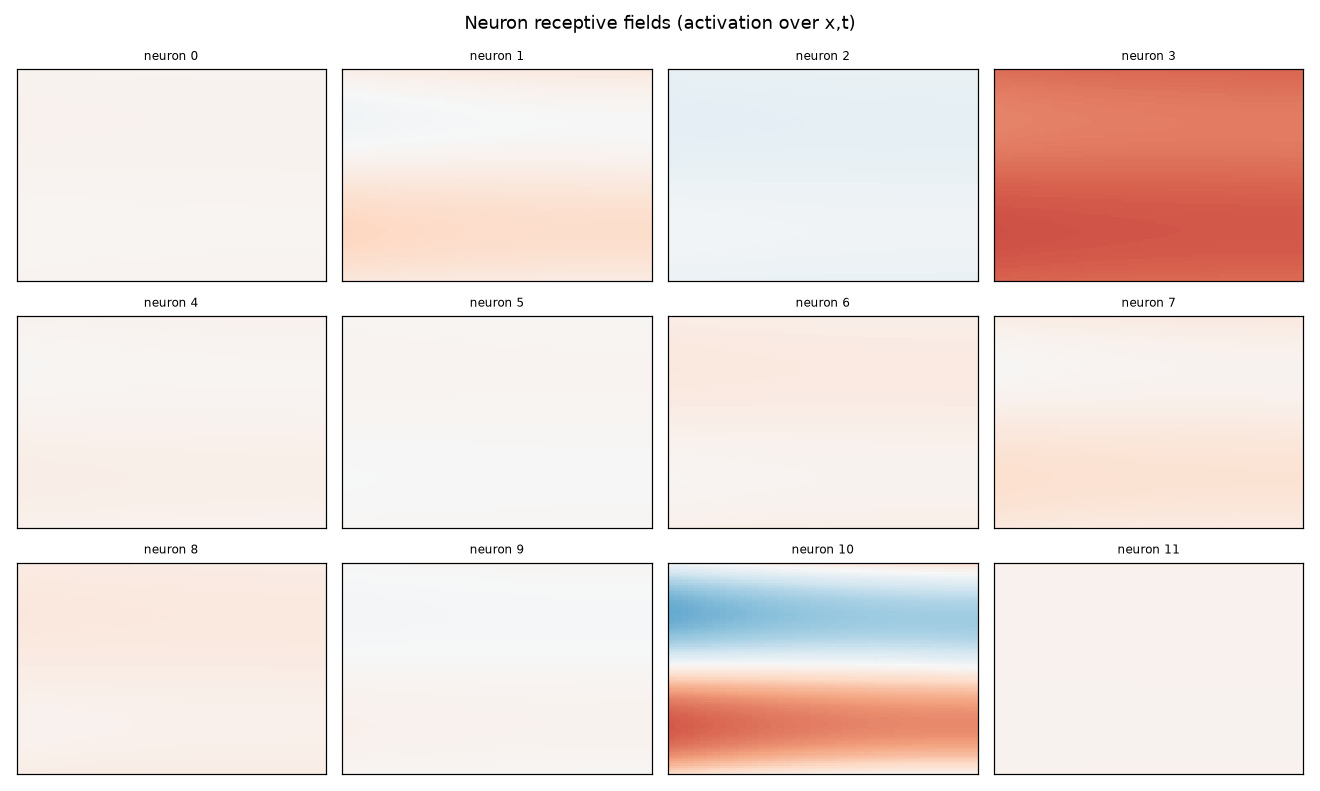
\includegraphics[width=\textwidth]{abl_meas_single/figures/neurons.png}
\caption{\textbf{abl\_meas\_single} --- Classical post-net neurons: receptive fields over $(x,t)$ and each neuron's dominant spatial frequency / effective rank.}
\end{figure}
\begin{figure}[H]\centering
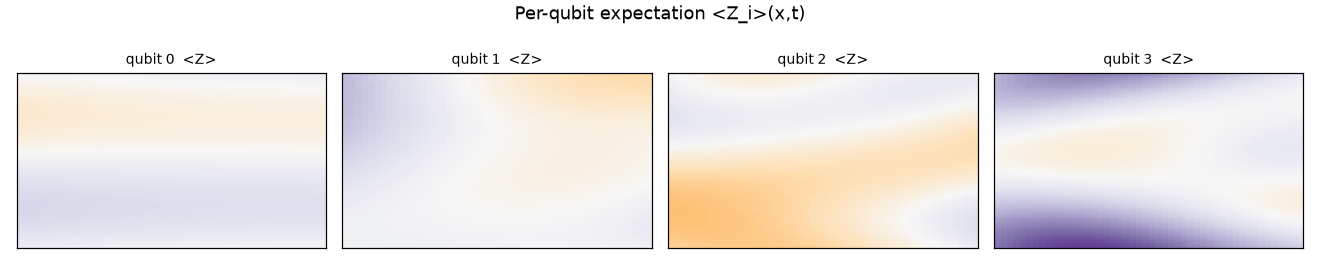
\includegraphics[width=\textwidth]{abl_meas_single/figures/qubits.png}
\caption{\textbf{abl\_meas\_single} --- Per-qubit $\langle Z\rangle$ receptive fields --- what feature each qubit computes over the domain (quantum models only).}
\end{figure}
\begin{figure}[H]\centering
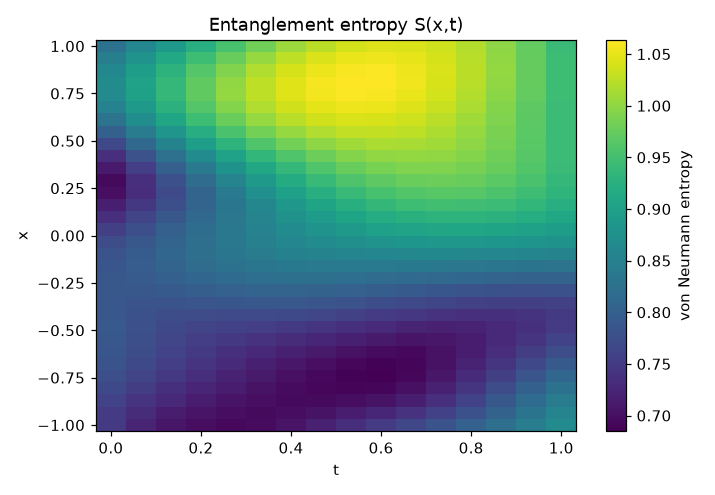
\includegraphics[width=\textwidth]{abl_meas_single/figures/entanglement.png}
\caption{\textbf{abl\_meas\_single} --- Von Neumann entanglement entropy $S(x,t)$ of a qubit bipartition across the domain (quantum models only).}
\end{figure}
\begin{figure}[H]\centering
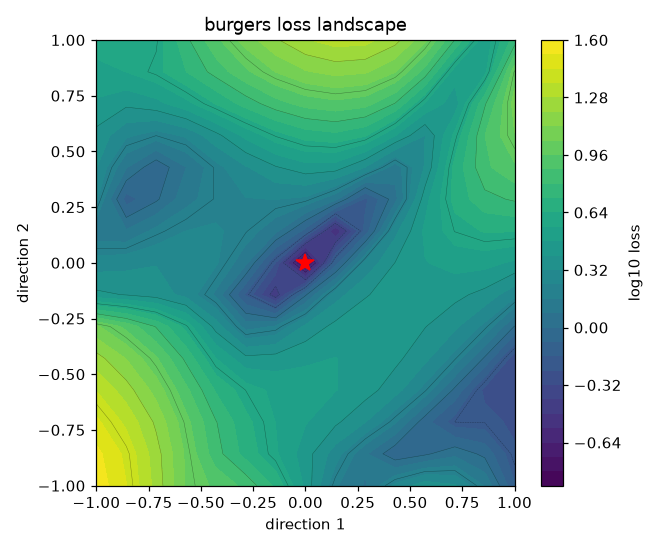
\includegraphics[width=\textwidth]{abl_meas_single/figures/landscape.png}
\caption{\textbf{abl\_meas\_single} --- Filter-normalized 2-D loss landscape around the trained minimum (Li et al.\ 2018). Flat/wide vs.\ sharp basin.}
\end{figure}
\begin{figure}[H]\centering
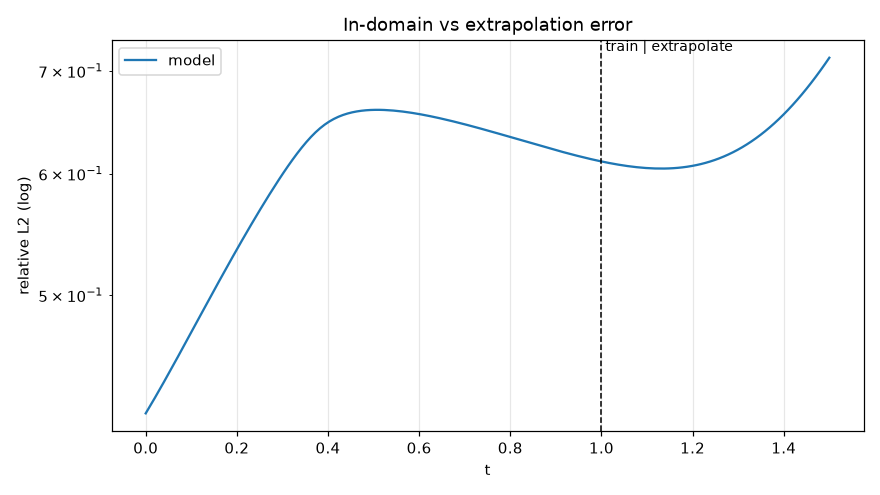
\includegraphics[width=\textwidth]{abl_meas_single/figures/generalization.png}
\caption{\textbf{abl\_meas\_single} --- Extrapolation: relative $L_2$ vs.\ $t$ beyond the $t\in[0,1]$ training window --- the off-domain penalty.}
\end{figure}
\begin{figure}[H]\centering
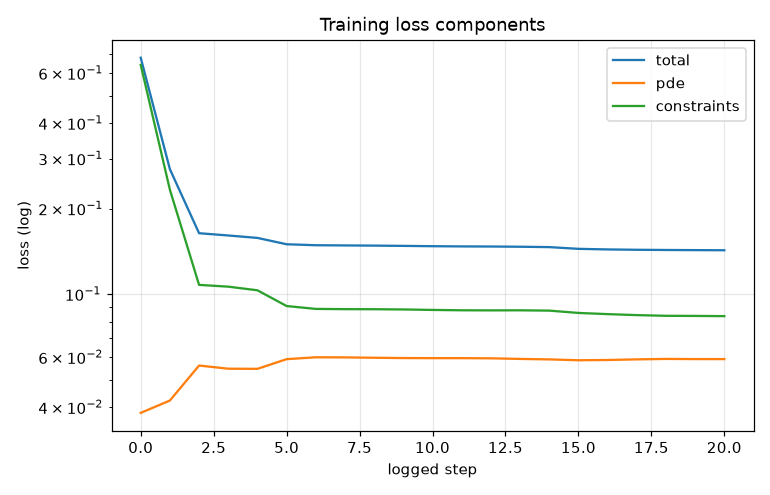
\includegraphics[width=\textwidth]{abl_meas_single/figures/loss.png}
\caption{\textbf{abl\_meas\_single} --- Training loss history (total, PDE-residual, and constraint terms).}
\end{figure}
\clearpage
\subsection{abl\_meas\_zz}
\noindent\small \textbf{rel-$L_2$}: 0.4723  \textbf{params}: 169  \textbf{PDE}: burgers  \textbf{Adam iters}: 2000  \textbf{seed}: 0  \textbf{model}: qapinn  \textbf{final PDE loss}: 4.07e-02  \textbf{wall time (s)}: 1797  \textbf{VQC}: 4q x3L ent=linear meas=zz scale=1.0\normalsize

\noindent\textbf{Observation.} ZZ-correlator readout restores amplitude close to the multi-qubit baseline: prediction spans +/-0.65 and snapshot model peaks reach \textasciitilde{}0.58, clearly better than the single-Z run. The qubits panel shows 4 \textless{}Z\_i\textgreater{} maps, the shock error fan reaches \textasciitilde{}0.9, and entanglement entropy ranges \textasciitilde{}0.45 to 1.2 with a bright high-entropy corner at (t=0, x=0.9) and a dark low-entropy pocket near (t=1.0, x=-0.8). The Fourier spectrum follows the reference through the first several harmonics before the usual high-k roll-off. Inference: two-qubit ZZ observables carry substantially more expressive power than single-Z, recovering near-baseline accuracy and making readout richness more impactful than raw qubit count.

\begin{figure}[H]\centering
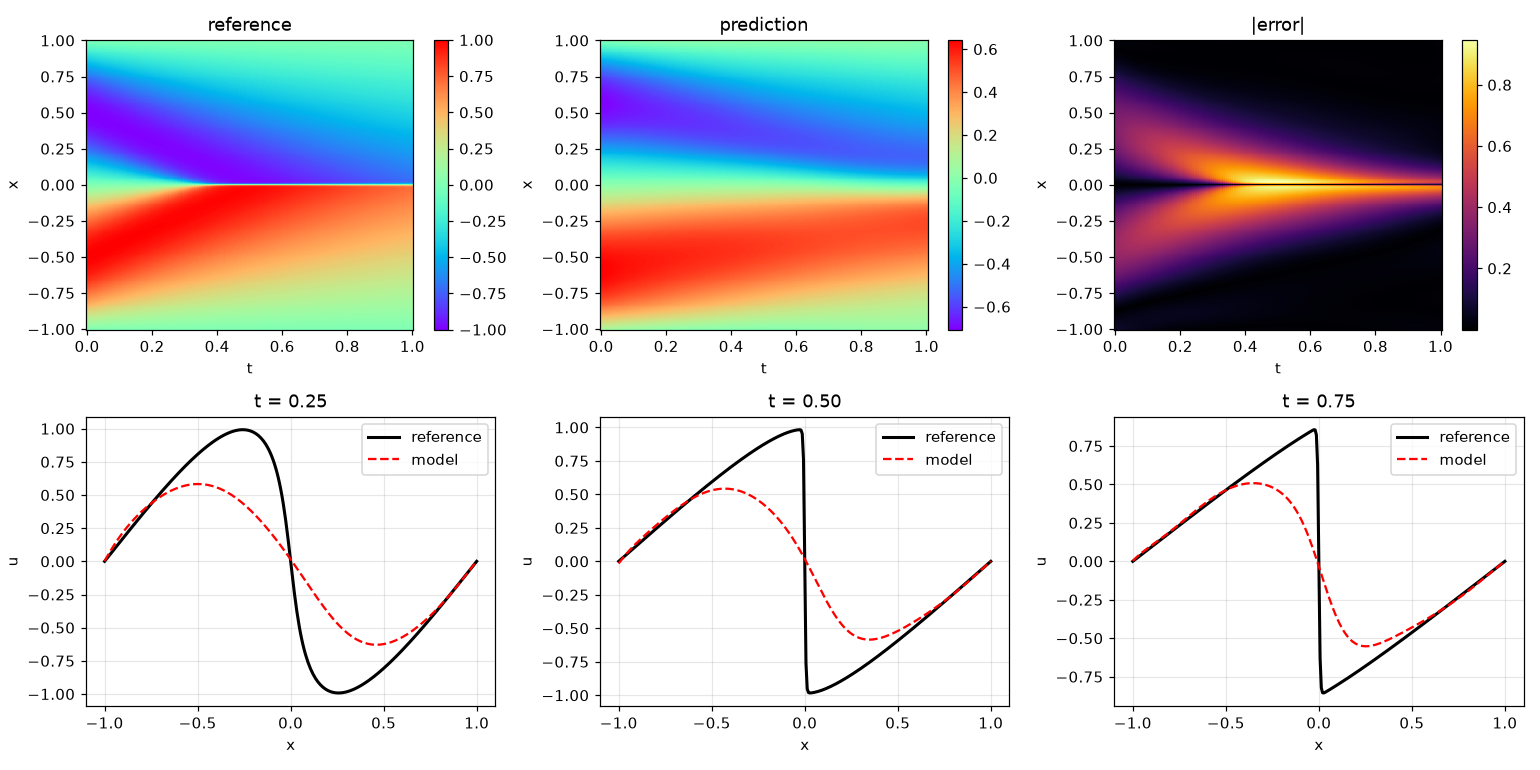
\includegraphics[width=\textwidth]{abl_meas_zz/figures/solution.png}
\caption{\textbf{abl\_meas\_zz} --- Predicted field $u(x,t)$ vs.\ exact reference, with the pointwise error map. The shock ($x\!=\!0$) is where a smooth network struggles.}
\end{figure}
\begin{figure}[H]\centering
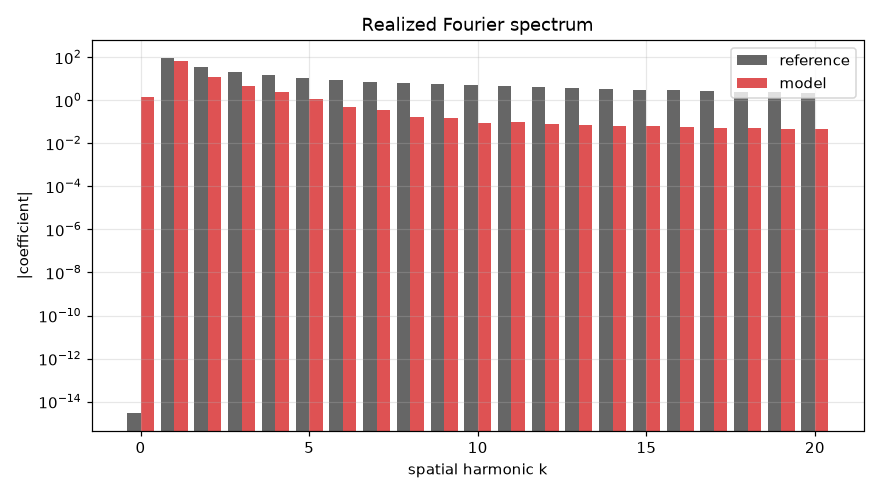
\includegraphics[width=\textwidth]{abl_meas_zz/figures/spectrum.png}
\caption{\textbf{abl\_meas\_zz} --- Realized spatial spectrum (per-harmonic magnitude) vs.\ reference. Tests whether the model captures the high-$k$ shock tail or only low frequencies.}
\end{figure}
\begin{figure}[H]\centering
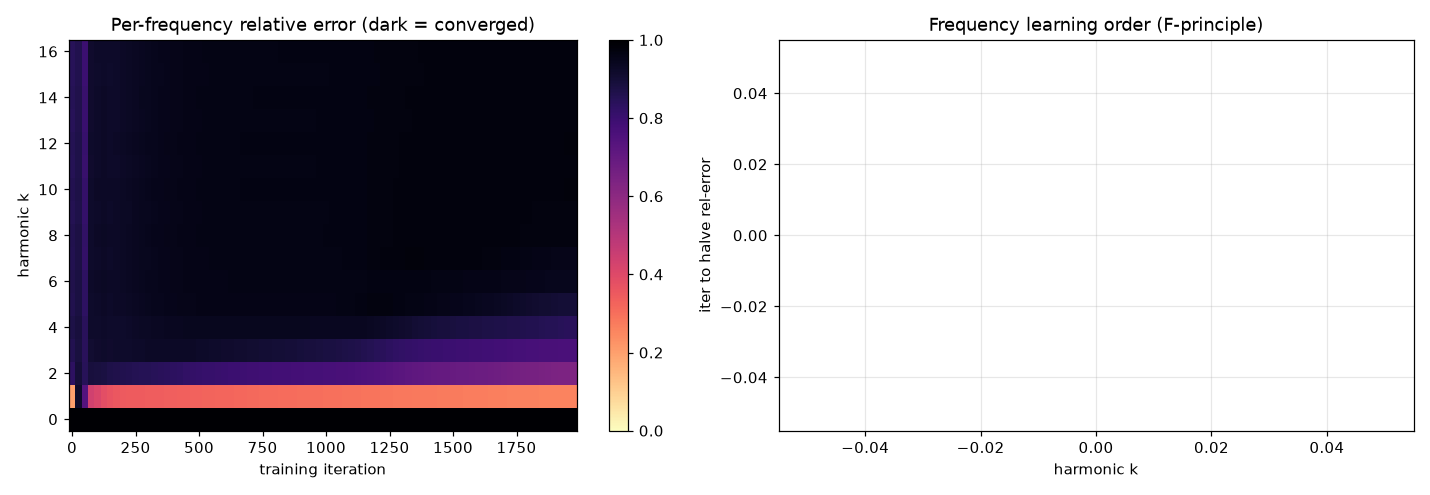
\includegraphics[width=\textwidth]{abl_meas_zz/figures/fprinciple.png}
\caption{\textbf{abl\_meas\_zz} --- F-principle heat-map: iteration at which each harmonic's relative error halves. Low harmonics converging first is the F-principle signature.}
\end{figure}
\begin{figure}[H]\centering
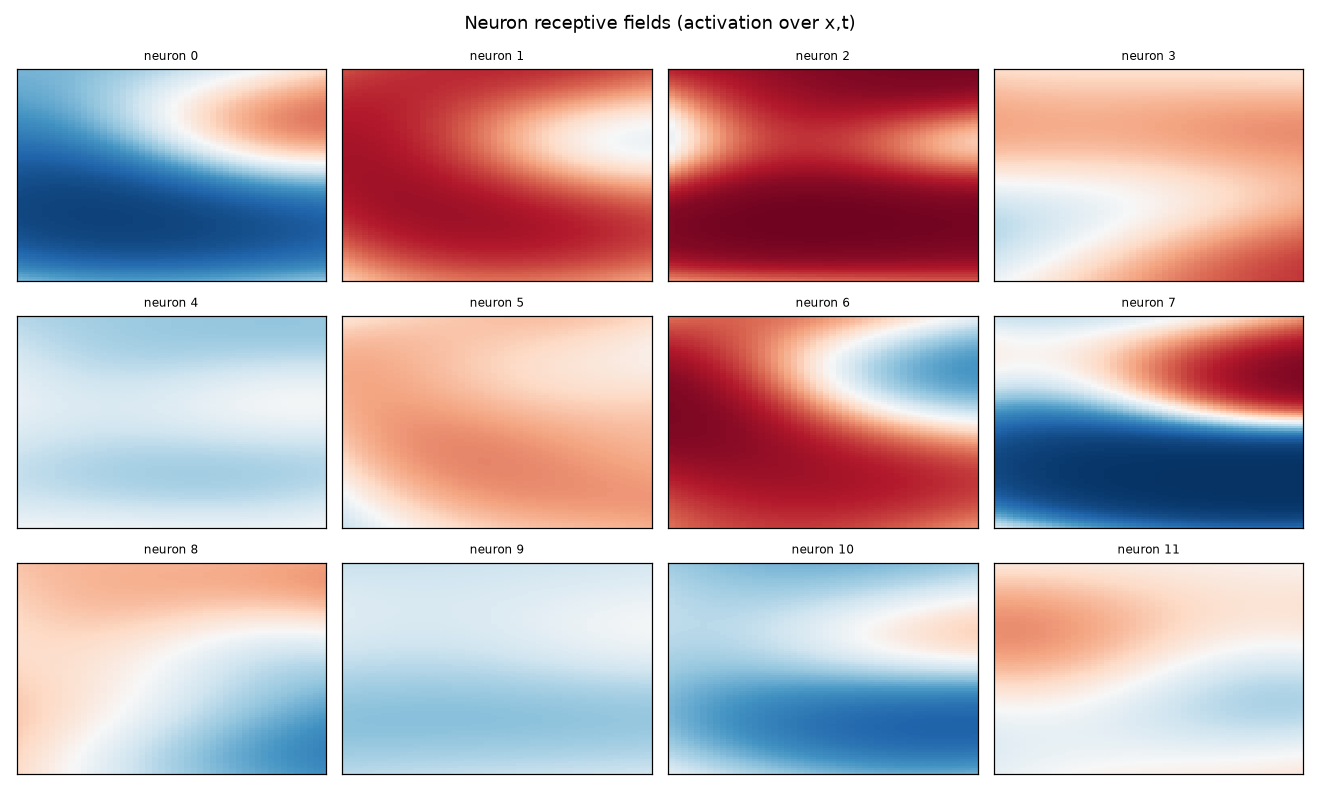
\includegraphics[width=\textwidth]{abl_meas_zz/figures/neurons.png}
\caption{\textbf{abl\_meas\_zz} --- Classical post-net neurons: receptive fields over $(x,t)$ and each neuron's dominant spatial frequency / effective rank.}
\end{figure}
\begin{figure}[H]\centering
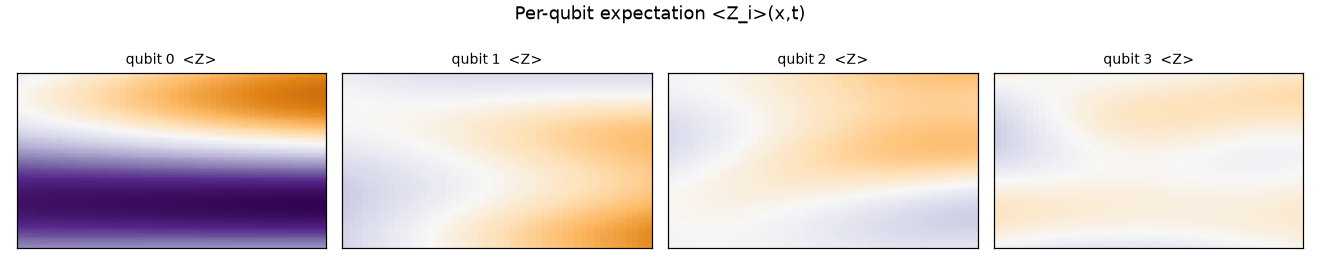
\includegraphics[width=\textwidth]{abl_meas_zz/figures/qubits.png}
\caption{\textbf{abl\_meas\_zz} --- Per-qubit $\langle Z\rangle$ receptive fields --- what feature each qubit computes over the domain (quantum models only).}
\end{figure}
\begin{figure}[H]\centering
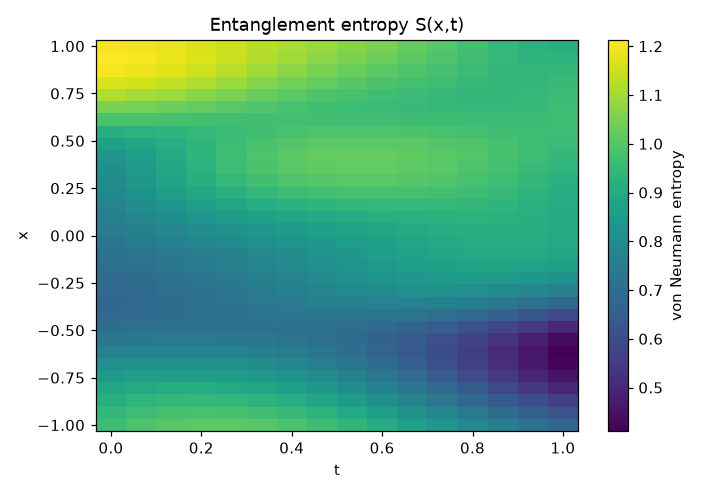
\includegraphics[width=\textwidth]{abl_meas_zz/figures/entanglement.png}
\caption{\textbf{abl\_meas\_zz} --- Von Neumann entanglement entropy $S(x,t)$ of a qubit bipartition across the domain (quantum models only).}
\end{figure}
\begin{figure}[H]\centering
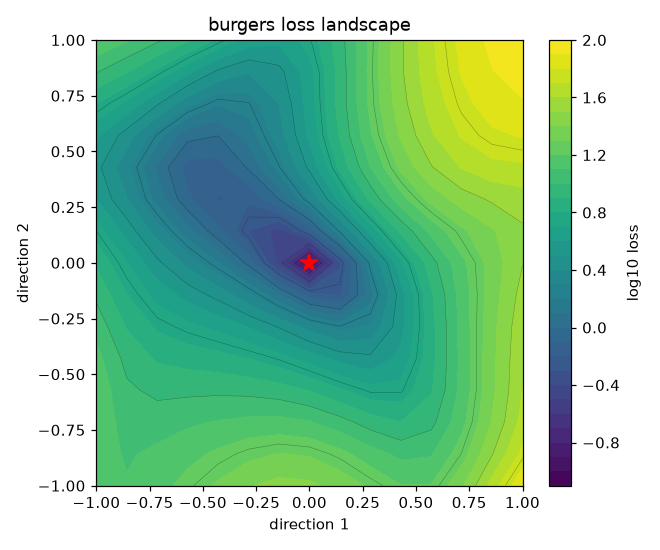
\includegraphics[width=\textwidth]{abl_meas_zz/figures/landscape.png}
\caption{\textbf{abl\_meas\_zz} --- Filter-normalized 2-D loss landscape around the trained minimum (Li et al.\ 2018). Flat/wide vs.\ sharp basin.}
\end{figure}
\begin{figure}[H]\centering
\includegraphics[width=\textwidth]{abl_meas_zz/figures/generalization.png}
\caption{\textbf{abl\_meas\_zz} --- Extrapolation: relative $L_2$ vs.\ $t$ beyond the $t\in[0,1]$ training window --- the off-domain penalty.}
\end{figure}
\begin{figure}[H]\centering
\includegraphics[width=\textwidth]{abl_meas_zz/figures/loss.png}
\caption{\textbf{abl\_meas\_zz} --- Training loss history (total, PDE-residual, and constraint terms).}
\end{figure}
\clearpage
\section{Tier-3 ablation --- encoding input scale (the $2\pi$ collapse)}
Scaling the encoding angle. Optimum near 1 (reference); at $2\pi$ the model collapses to the trivial solution --- the black-hole trainability pathology made concrete.

\subsection{abl\_scale\_05}
\noindent\small \textbf{rel-$L_2$}: 0.5134  \textbf{params}: 121  \textbf{PDE}: burgers  \textbf{Adam iters}: 2000  \textbf{seed}: 0  \textbf{model}: qapinn  \textbf{final PDE loss}: 4.81e-02  \textbf{wall time (s)}: 1892  \textbf{VQC}: 4q x3L ent=linear meas=multi scale=0.5\normalsize

\noindent\textbf{Observation.} With input\_scale=0.5 the encoding under-activates: prediction is only +/-0.5 and snapshot model peaks \textasciitilde{}0.50, the lowest-amplitude smooth fit of the scale sweep. The 4 qubit \textless{}Z\_i\textgreater{} maps are very smooth and low-contrast (mostly pale purple, little orange), and entanglement entropy is smooth and modest (\textasciitilde{}0.53 to 0.95), increasing left-to-right in t toward a bright band around x=0. The error fan at x=0 reaches \textasciitilde{}0.9 and the spectrum shows the model decaying faster than reference beyond k\textasciitilde{}4. Inference: a small encoding scale compresses the input into a near-linear region of the feature map, limiting accessible frequencies and yielding an under-fit, over-smooth solution.

\begin{figure}[H]\centering
\includegraphics[width=\textwidth]{abl_scale_05/figures/solution.png}
\caption{\textbf{abl\_scale\_05} --- Predicted field $u(x,t)$ vs.\ exact reference, with the pointwise error map. The shock ($x\!=\!0$) is where a smooth network struggles.}
\end{figure}
\begin{figure}[H]\centering
\includegraphics[width=\textwidth]{abl_scale_05/figures/spectrum.png}
\caption{\textbf{abl\_scale\_05} --- Realized spatial spectrum (per-harmonic magnitude) vs.\ reference. Tests whether the model captures the high-$k$ shock tail or only low frequencies.}
\end{figure}
\begin{figure}[H]\centering
\includegraphics[width=\textwidth]{abl_scale_05/figures/fprinciple.png}
\caption{\textbf{abl\_scale\_05} --- F-principle heat-map: iteration at which each harmonic's relative error halves. Low harmonics converging first is the F-principle signature.}
\end{figure}
\begin{figure}[H]\centering
\includegraphics[width=\textwidth]{abl_scale_05/figures/neurons.png}
\caption{\textbf{abl\_scale\_05} --- Classical post-net neurons: receptive fields over $(x,t)$ and each neuron's dominant spatial frequency / effective rank.}
\end{figure}
\begin{figure}[H]\centering
\includegraphics[width=\textwidth]{abl_scale_05/figures/qubits.png}
\caption{\textbf{abl\_scale\_05} --- Per-qubit $\langle Z\rangle$ receptive fields --- what feature each qubit computes over the domain (quantum models only).}
\end{figure}
\begin{figure}[H]\centering
\includegraphics[width=\textwidth]{abl_scale_05/figures/entanglement.png}
\caption{\textbf{abl\_scale\_05} --- Von Neumann entanglement entropy $S(x,t)$ of a qubit bipartition across the domain (quantum models only).}
\end{figure}
\begin{figure}[H]\centering
\includegraphics[width=\textwidth]{abl_scale_05/figures/landscape.png}
\caption{\textbf{abl\_scale\_05} --- Filter-normalized 2-D loss landscape around the trained minimum (Li et al.\ 2018). Flat/wide vs.\ sharp basin.}
\end{figure}
\begin{figure}[H]\centering
\includegraphics[width=\textwidth]{abl_scale_05/figures/generalization.png}
\caption{\textbf{abl\_scale\_05} --- Extrapolation: relative $L_2$ vs.\ $t$ beyond the $t\in[0,1]$ training window --- the off-domain penalty.}
\end{figure}
\begin{figure}[H]\centering
\includegraphics[width=\textwidth]{abl_scale_05/figures/loss.png}
\caption{\textbf{abl\_scale\_05} --- Training loss history (total, PDE-residual, and constraint terms).}
\end{figure}
\clearpage
\subsection{abl\_scale\_pi}
\noindent\small \textbf{rel-$L_2$}: 0.5164  \textbf{params}: 121  \textbf{PDE}: burgers  \textbf{Adam iters}: 2000  \textbf{seed}: 0  \textbf{model}: qapinn  \textbf{final PDE loss}: 7.46e-02  \textbf{wall time (s)}: 1995  \textbf{VQC}: 4q x3L ent=linear meas=multi scale=3.14159\normalsize

\noindent\textbf{Observation.} At input\_scale=pi the prediction (+/-0.5) becomes visibly noisy: the 2D map shows patchy blotches instead of the clean two-lobe structure, and snapshot model curves (\textasciitilde{}0.47 peak) carry small oscillatory wiggles rather than a smooth arc. The 4 qubit \textless{}Z\_i\textgreater{} maps display clear mid-frequency oscillations/banding, and entanglement entropy is patchy and disordered, ranging \textasciitilde{}0.2 to 1.1 with scattered dark and bright cells rather than smooth gradients. The error fan at x=0 reaches \textasciitilde{}0.85. Inference: pushing the encoding scale to pi begins to over-fold the input, injecting spurious high-frequency content and marking the onset of the instability that fully collapses at 2pi.

\begin{figure}[H]\centering
\includegraphics[width=\textwidth]{abl_scale_pi/figures/solution.png}
\caption{\textbf{abl\_scale\_pi} --- Predicted field $u(x,t)$ vs.\ exact reference, with the pointwise error map. The shock ($x\!=\!0$) is where a smooth network struggles.}
\end{figure}
\begin{figure}[H]\centering
\includegraphics[width=\textwidth]{abl_scale_pi/figures/spectrum.png}
\caption{\textbf{abl\_scale\_pi} --- Realized spatial spectrum (per-harmonic magnitude) vs.\ reference. Tests whether the model captures the high-$k$ shock tail or only low frequencies.}
\end{figure}
\begin{figure}[H]\centering
\includegraphics[width=\textwidth]{abl_scale_pi/figures/fprinciple.png}
\caption{\textbf{abl\_scale\_pi} --- F-principle heat-map: iteration at which each harmonic's relative error halves. Low harmonics converging first is the F-principle signature.}
\end{figure}
\begin{figure}[H]\centering
\includegraphics[width=\textwidth]{abl_scale_pi/figures/neurons.png}
\caption{\textbf{abl\_scale\_pi} --- Classical post-net neurons: receptive fields over $(x,t)$ and each neuron's dominant spatial frequency / effective rank.}
\end{figure}
\begin{figure}[H]\centering
\includegraphics[width=\textwidth]{abl_scale_pi/figures/qubits.png}
\caption{\textbf{abl\_scale\_pi} --- Per-qubit $\langle Z\rangle$ receptive fields --- what feature each qubit computes over the domain (quantum models only).}
\end{figure}
\begin{figure}[H]\centering
\includegraphics[width=\textwidth]{abl_scale_pi/figures/entanglement.png}
\caption{\textbf{abl\_scale\_pi} --- Von Neumann entanglement entropy $S(x,t)$ of a qubit bipartition across the domain (quantum models only).}
\end{figure}
\begin{figure}[H]\centering
\includegraphics[width=\textwidth]{abl_scale_pi/figures/landscape.png}
\caption{\textbf{abl\_scale\_pi} --- Filter-normalized 2-D loss landscape around the trained minimum (Li et al.\ 2018). Flat/wide vs.\ sharp basin.}
\end{figure}
\begin{figure}[H]\centering
\includegraphics[width=\textwidth]{abl_scale_pi/figures/generalization.png}
\caption{\textbf{abl\_scale\_pi} --- Extrapolation: relative $L_2$ vs.\ $t$ beyond the $t\in[0,1]$ training window --- the off-domain penalty.}
\end{figure}
\begin{figure}[H]\centering
\includegraphics[width=\textwidth]{abl_scale_pi/figures/loss.png}
\caption{\textbf{abl\_scale\_pi} --- Training loss history (total, PDE-residual, and constraint terms).}
\end{figure}
\clearpage
\subsection{abl\_scale\_2pi}
\noindent\small \textbf{rel-$L_2$}: 1.0003  \textbf{params}: 121  \textbf{PDE}: burgers  \textbf{Adam iters}: 2000  \textbf{seed}: 0  \textbf{model}: qapinn  \textbf{final PDE loss}: 3.13e-04  \textbf{wall time (s)}: 1968  \textbf{VQC}: 4q x3L ent=linear meas=multi scale=6.28318\normalsize

\noindent\textbf{Observation.} Collapse confirmed: the prediction colorbar spans only about -0.015 to -0.002 (|u| \textasciitilde{} 0.01, effectively zero) and shows fine speckled noise, while all three snapshot model lines are flat at u \textasciitilde{} 0 straight across, completely missing the reference sawtooth. Because the prediction is \textasciitilde{}0, the |error| map equals the reference amplitude with the colorbar saturating at 1.0, and the Fourier spectrum shows the model k\textgreater{}=1 harmonics collapsed to \textasciitilde{}1e-2 to 1e-1, far below the reference bars. The 4 qubit \textless{}Z\_i\textgreater{} maps are dominated by high-frequency horizontal striping (aliasing) and entanglement entropy is fully disordered noise (\textasciitilde{}0.3 to 1.1). Inference: input\_scale=2pi aliases the encoding so severely that the optimizer finds only the trivial u\textasciitilde{}0 solution, a total collapse consistent with the expected failure mode.

\begin{figure}[H]\centering
\includegraphics[width=\textwidth]{abl_scale_2pi/figures/solution.png}
\caption{\textbf{abl\_scale\_2pi} --- Predicted field $u(x,t)$ vs.\ exact reference, with the pointwise error map. The shock ($x\!=\!0$) is where a smooth network struggles.}
\end{figure}
\begin{figure}[H]\centering
\includegraphics[width=\textwidth]{abl_scale_2pi/figures/spectrum.png}
\caption{\textbf{abl\_scale\_2pi} --- Realized spatial spectrum (per-harmonic magnitude) vs.\ reference. Tests whether the model captures the high-$k$ shock tail or only low frequencies.}
\end{figure}
\begin{figure}[H]\centering
\includegraphics[width=\textwidth]{abl_scale_2pi/figures/fprinciple.png}
\caption{\textbf{abl\_scale\_2pi} --- F-principle heat-map: iteration at which each harmonic's relative error halves. Low harmonics converging first is the F-principle signature.}
\end{figure}
\begin{figure}[H]\centering
\includegraphics[width=\textwidth]{abl_scale_2pi/figures/neurons.png}
\caption{\textbf{abl\_scale\_2pi} --- Classical post-net neurons: receptive fields over $(x,t)$ and each neuron's dominant spatial frequency / effective rank.}
\end{figure}
\begin{figure}[H]\centering
\includegraphics[width=\textwidth]{abl_scale_2pi/figures/qubits.png}
\caption{\textbf{abl\_scale\_2pi} --- Per-qubit $\langle Z\rangle$ receptive fields --- what feature each qubit computes over the domain (quantum models only).}
\end{figure}
\begin{figure}[H]\centering
\includegraphics[width=\textwidth]{abl_scale_2pi/figures/entanglement.png}
\caption{\textbf{abl\_scale\_2pi} --- Von Neumann entanglement entropy $S(x,t)$ of a qubit bipartition across the domain (quantum models only).}
\end{figure}
\begin{figure}[H]\centering
\includegraphics[width=\textwidth]{abl_scale_2pi/figures/landscape.png}
\caption{\textbf{abl\_scale\_2pi} --- Filter-normalized 2-D loss landscape around the trained minimum (Li et al.\ 2018). Flat/wide vs.\ sharp basin.}
\end{figure}
\begin{figure}[H]\centering
\includegraphics[width=\textwidth]{abl_scale_2pi/figures/generalization.png}
\caption{\textbf{abl\_scale\_2pi} --- Extrapolation: relative $L_2$ vs.\ $t$ beyond the $t\in[0,1]$ training window --- the off-domain penalty.}
\end{figure}
\begin{figure}[H]\centering
\includegraphics[width=\textwidth]{abl_scale_2pi/figures/loss.png}
\caption{\textbf{abl\_scale\_2pi} --- Training loss history (total, PDE-residual, and constraint terms).}
\end{figure}
\clearpage
\section{Matched classical controls (cPINN)}
Param-matched tanh MLPs [2,a,b,1] --- the fair-capacity baseline each QAPINN is compared against.

\subsection{abl\_cls\_29}
\noindent\small \textbf{rel-$L_2$}: 0.5325  \textbf{params}: 29  \textbf{PDE}: burgers  \textbf{Adam iters}: 2000  \textbf{seed}: 0  \textbf{model}: classical  \textbf{final PDE loss}: 5.21e-02  \textbf{wall time (s)}: 15\normalsize

\noindent\textbf{Observation.} Smallest net: the shock is entirely erased into a smooth low-amplitude sine, with the model peak capped at about +-0.55 versus the reference +-1.0, and the t=0.50 near-vertical front replaced by a gentle slope. Error is a bright plume emanating from x=0 that grows with t and biases to the +x side, peaking near |error|\textasciitilde{}0.9. Spectrum: model matches only the k=1 fundamental (\textasciitilde{}60 vs reference \textasciitilde{}80) and every harmonic k\textgreater{}=2 sits well below reference, dropping \textasciitilde{}1-2 decades low by k\textgreater{}=4 (also a spurious nonzero k=0 mean \textasciitilde{}2). Inference: at this capacity the network only fits the smooth envelope and has zero shock resolution.

\begin{figure}[H]\centering
\includegraphics[width=\textwidth]{abl_cls_29/figures/solution.png}
\caption{\textbf{abl\_cls\_29} --- Predicted field $u(x,t)$ vs.\ exact reference, with the pointwise error map. The shock ($x\!=\!0$) is where a smooth network struggles.}
\end{figure}
\begin{figure}[H]\centering
\includegraphics[width=\textwidth]{abl_cls_29/figures/spectrum.png}
\caption{\textbf{abl\_cls\_29} --- Realized spatial spectrum (per-harmonic magnitude) vs.\ reference. Tests whether the model captures the high-$k$ shock tail or only low frequencies.}
\end{figure}
\begin{figure}[H]\centering
\includegraphics[width=\textwidth]{abl_cls_29/figures/fprinciple.png}
\caption{\textbf{abl\_cls\_29} --- F-principle heat-map: iteration at which each harmonic's relative error halves. Low harmonics converging first is the F-principle signature.}
\end{figure}
\begin{figure}[H]\centering
\includegraphics[width=\textwidth]{abl_cls_29/figures/neurons.png}
\caption{\textbf{abl\_cls\_29} --- Classical post-net neurons: receptive fields over $(x,t)$ and each neuron's dominant spatial frequency / effective rank.}
\end{figure}
\begin{figure}[H]\centering
\includegraphics[width=\textwidth]{abl_cls_29/figures/landscape.png}
\caption{\textbf{abl\_cls\_29} --- Filter-normalized 2-D loss landscape around the trained minimum (Li et al.\ 2018). Flat/wide vs.\ sharp basin.}
\end{figure}
\begin{figure}[H]\centering
\includegraphics[width=\textwidth]{abl_cls_29/figures/generalization.png}
\caption{\textbf{abl\_cls\_29} --- Extrapolation: relative $L_2$ vs.\ $t$ beyond the $t\in[0,1]$ training window --- the off-domain penalty.}
\end{figure}
\begin{figure}[H]\centering
\includegraphics[width=\textwidth]{abl_cls_29/figures/loss.png}
\caption{\textbf{abl\_cls\_29} --- Training loss history (total, PDE-residual, and constraint terms).}
\end{figure}
\clearpage
\subsection{abl\_cls\_73}
\noindent\small \textbf{rel-$L_2$}: 0.5334  \textbf{params}: 73  \textbf{PDE}: burgers  \textbf{Adam iters}: 2000  \textbf{seed}: 0  \textbf{model}: classical  \textbf{final PDE loss}: 4.81e-02  \textbf{wall time (s)}: 13\normalsize

\noindent\textbf{Observation.} Almost indistinguishable from the 29-param run: amplitude capped at \textasciitilde{}+-0.57, the shock at t=0.50 rounded to a smooth curve with no discontinuity, and error concentrated in the same x\textasciitilde{}0 plume peaking \textasciitilde{}0.9. Spectrum tracks k=1 (\textasciitilde{}60 vs 80) but falls monotonically below reference from k=2 onward, roughly 1 decade low across k=6-20. Inference: doubling params from 29 buys no visible shock sharpening.

\begin{figure}[H]\centering
\includegraphics[width=\textwidth]{abl_cls_73/figures/solution.png}
\caption{\textbf{abl\_cls\_73} --- Predicted field $u(x,t)$ vs.\ exact reference, with the pointwise error map. The shock ($x\!=\!0$) is where a smooth network struggles.}
\end{figure}
\begin{figure}[H]\centering
\includegraphics[width=\textwidth]{abl_cls_73/figures/spectrum.png}
\caption{\textbf{abl\_cls\_73} --- Realized spatial spectrum (per-harmonic magnitude) vs.\ reference. Tests whether the model captures the high-$k$ shock tail or only low frequencies.}
\end{figure}
\begin{figure}[H]\centering
\includegraphics[width=\textwidth]{abl_cls_73/figures/fprinciple.png}
\caption{\textbf{abl\_cls\_73} --- F-principle heat-map: iteration at which each harmonic's relative error halves. Low harmonics converging first is the F-principle signature.}
\end{figure}
\begin{figure}[H]\centering
\includegraphics[width=\textwidth]{abl_cls_73/figures/neurons.png}
\caption{\textbf{abl\_cls\_73} --- Classical post-net neurons: receptive fields over $(x,t)$ and each neuron's dominant spatial frequency / effective rank.}
\end{figure}
\begin{figure}[H]\centering
\includegraphics[width=\textwidth]{abl_cls_73/figures/landscape.png}
\caption{\textbf{abl\_cls\_73} --- Filter-normalized 2-D loss landscape around the trained minimum (Li et al.\ 2018). Flat/wide vs.\ sharp basin.}
\end{figure}
\begin{figure}[H]\centering
\includegraphics[width=\textwidth]{abl_cls_73/figures/generalization.png}
\caption{\textbf{abl\_cls\_73} --- Extrapolation: relative $L_2$ vs.\ $t$ beyond the $t\in[0,1]$ training window --- the off-domain penalty.}
\end{figure}
\begin{figure}[H]\centering
\includegraphics[width=\textwidth]{abl_cls_73/figures/loss.png}
\caption{\textbf{abl\_cls\_73} --- Training loss history (total, PDE-residual, and constraint terms).}
\end{figure}
\clearpage
\subsection{abl\_cls\_99}
\noindent\small \textbf{rel-$L_2$}: 0.4701  \textbf{params}: 99  \textbf{PDE}: burgers  \textbf{Adam iters}: 2000  \textbf{seed}: 0  \textbf{model}: classical  \textbf{final PDE loss}: 3.29e-02  \textbf{wall time (s)}: 21\normalsize

\noindent\textbf{Observation.} Noticeably better: amplitude reaches \textasciitilde{}+-0.73 and the front becomes asymmetric/tilted (steeper just left of x=0 with an inflection at x\textasciitilde{}0) rather than a symmetric sine, so it begins to hint at the shock. Error plume peak is a bit higher (\textasciitilde{}1.05) but the low-x region is cleaner, and the spectrum keeps model bars within \textasciitilde{}factor 3 of reference out to about k=6-7 before rolling off. Inference: this mid-count net is the first to partially resolve the shock geometry, not just the envelope.

\begin{figure}[H]\centering
\includegraphics[width=\textwidth]{abl_cls_99/figures/solution.png}
\caption{\textbf{abl\_cls\_99} --- Predicted field $u(x,t)$ vs.\ exact reference, with the pointwise error map. The shock ($x\!=\!0$) is where a smooth network struggles.}
\end{figure}
\begin{figure}[H]\centering
\includegraphics[width=\textwidth]{abl_cls_99/figures/spectrum.png}
\caption{\textbf{abl\_cls\_99} --- Realized spatial spectrum (per-harmonic magnitude) vs.\ reference. Tests whether the model captures the high-$k$ shock tail or only low frequencies.}
\end{figure}
\begin{figure}[H]\centering
\includegraphics[width=\textwidth]{abl_cls_99/figures/fprinciple.png}
\caption{\textbf{abl\_cls\_99} --- F-principle heat-map: iteration at which each harmonic's relative error halves. Low harmonics converging first is the F-principle signature.}
\end{figure}
\begin{figure}[H]\centering
\includegraphics[width=\textwidth]{abl_cls_99/figures/neurons.png}
\caption{\textbf{abl\_cls\_99} --- Classical post-net neurons: receptive fields over $(x,t)$ and each neuron's dominant spatial frequency / effective rank.}
\end{figure}
\begin{figure}[H]\centering
\includegraphics[width=\textwidth]{abl_cls_99/figures/landscape.png}
\caption{\textbf{abl\_cls\_99} --- Filter-normalized 2-D loss landscape around the trained minimum (Li et al.\ 2018). Flat/wide vs.\ sharp basin.}
\end{figure}
\begin{figure}[H]\centering
\includegraphics[width=\textwidth]{abl_cls_99/figures/generalization.png}
\caption{\textbf{abl\_cls\_99} --- Extrapolation: relative $L_2$ vs.\ $t$ beyond the $t\in[0,1]$ training window --- the off-domain penalty.}
\end{figure}
\begin{figure}[H]\centering
\includegraphics[width=\textwidth]{abl_cls_99/figures/loss.png}
\caption{\textbf{abl\_cls\_99} --- Training loss history (total, PDE-residual, and constraint terms).}
\end{figure}
\clearpage
\subsection{abl\_cls\_105}
\noindent\small \textbf{rel-$L_2$}: 0.5225  \textbf{params}: 105  \textbf{PDE}: burgers  \textbf{Adam iters}: 2000  \textbf{seed}: 0  \textbf{model}: classical  \textbf{final PDE loss}: 4.78e-02  \textbf{wall time (s)}: 12\normalsize

\noindent\textbf{Observation.} Regresses relative to 99: amplitude back down to \textasciitilde{}+-0.55 and the front smoothed into a symmetric sine with no tilt. Error plume from x=0 peaks \textasciitilde{}0.9 and spreads on the +x side; spectrum matches k=1 (\textasciitilde{}50 vs 80) then falls \textasciitilde{}1 decade below reference for k\textgreater{}=4. Inference: more parameters than 99 here yield a worse, purely smooth fit, so capacity alone does not help the shock.

\begin{figure}[H]\centering
\includegraphics[width=\textwidth]{abl_cls_105/figures/solution.png}
\caption{\textbf{abl\_cls\_105} --- Predicted field $u(x,t)$ vs.\ exact reference, with the pointwise error map. The shock ($x\!=\!0$) is where a smooth network struggles.}
\end{figure}
\begin{figure}[H]\centering
\includegraphics[width=\textwidth]{abl_cls_105/figures/spectrum.png}
\caption{\textbf{abl\_cls\_105} --- Realized spatial spectrum (per-harmonic magnitude) vs.\ reference. Tests whether the model captures the high-$k$ shock tail or only low frequencies.}
\end{figure}
\begin{figure}[H]\centering
\includegraphics[width=\textwidth]{abl_cls_105/figures/fprinciple.png}
\caption{\textbf{abl\_cls\_105} --- F-principle heat-map: iteration at which each harmonic's relative error halves. Low harmonics converging first is the F-principle signature.}
\end{figure}
\begin{figure}[H]\centering
\includegraphics[width=\textwidth]{abl_cls_105/figures/neurons.png}
\caption{\textbf{abl\_cls\_105} --- Classical post-net neurons: receptive fields over $(x,t)$ and each neuron's dominant spatial frequency / effective rank.}
\end{figure}
\begin{figure}[H]\centering
\includegraphics[width=\textwidth]{abl_cls_105/figures/landscape.png}
\caption{\textbf{abl\_cls\_105} --- Filter-normalized 2-D loss landscape around the trained minimum (Li et al.\ 2018). Flat/wide vs.\ sharp basin.}
\end{figure}
\begin{figure}[H]\centering
\includegraphics[width=\textwidth]{abl_cls_105/figures/generalization.png}
\caption{\textbf{abl\_cls\_105} --- Extrapolation: relative $L_2$ vs.\ $t$ beyond the $t\in[0,1]$ training window --- the off-domain penalty.}
\end{figure}
\begin{figure}[H]\centering
\includegraphics[width=\textwidth]{abl_cls_105/figures/loss.png}
\caption{\textbf{abl\_cls\_105} --- Training loss history (total, PDE-residual, and constraint terms).}
\end{figure}
\clearpage
\subsection{abl\_cls\_113}
\noindent\small \textbf{rel-$L_2$}: 0.5016  \textbf{params}: 113  \textbf{PDE}: burgers  \textbf{Adam iters}: 2000  \textbf{seed}: 0  \textbf{model}: classical  \textbf{final PDE loss}: 4.59e-02  \textbf{wall time (s)}: 12\normalsize

\noindent\textbf{Observation.} Amplitude capped at \textasciitilde{}+-0.62, slightly higher than 105 but still a rounded front with no true steepening at t=0.50. Error stays in the x\textasciitilde{}0 plume (peak \textasciitilde{}0.85) biased to +x; spectrum tracks k=1 (\textasciitilde{}55 vs 80) and sits \textasciitilde{}0.5-1 decade below reference from k\textgreater{}=3 out to k=20. Inference: modest amplitude gain, still no shock resolution.

\begin{figure}[H]\centering
\includegraphics[width=\textwidth]{abl_cls_113/figures/solution.png}
\caption{\textbf{abl\_cls\_113} --- Predicted field $u(x,t)$ vs.\ exact reference, with the pointwise error map. The shock ($x\!=\!0$) is where a smooth network struggles.}
\end{figure}
\begin{figure}[H]\centering
\includegraphics[width=\textwidth]{abl_cls_113/figures/spectrum.png}
\caption{\textbf{abl\_cls\_113} --- Realized spatial spectrum (per-harmonic magnitude) vs.\ reference. Tests whether the model captures the high-$k$ shock tail or only low frequencies.}
\end{figure}
\begin{figure}[H]\centering
\includegraphics[width=\textwidth]{abl_cls_113/figures/fprinciple.png}
\caption{\textbf{abl\_cls\_113} --- F-principle heat-map: iteration at which each harmonic's relative error halves. Low harmonics converging first is the F-principle signature.}
\end{figure}
\begin{figure}[H]\centering
\includegraphics[width=\textwidth]{abl_cls_113/figures/neurons.png}
\caption{\textbf{abl\_cls\_113} --- Classical post-net neurons: receptive fields over $(x,t)$ and each neuron's dominant spatial frequency / effective rank.}
\end{figure}
\begin{figure}[H]\centering
\includegraphics[width=\textwidth]{abl_cls_113/figures/landscape.png}
\caption{\textbf{abl\_cls\_113} --- Filter-normalized 2-D loss landscape around the trained minimum (Li et al.\ 2018). Flat/wide vs.\ sharp basin.}
\end{figure}
\begin{figure}[H]\centering
\includegraphics[width=\textwidth]{abl_cls_113/figures/generalization.png}
\caption{\textbf{abl\_cls\_113} --- Extrapolation: relative $L_2$ vs.\ $t$ beyond the $t\in[0,1]$ training window --- the off-domain penalty.}
\end{figure}
\begin{figure}[H]\centering
\includegraphics[width=\textwidth]{abl_cls_113/figures/loss.png}
\caption{\textbf{abl\_cls\_113} --- Training loss history (total, PDE-residual, and constraint terms).}
\end{figure}
\clearpage
\subsection{abl\_cls\_121}
\noindent\small \textbf{rel-$L_2$}: 0.5349  \textbf{params}: 121  \textbf{PDE}: burgers  \textbf{Adam iters}: 2000  \textbf{seed}: 0  \textbf{model}: classical  \textbf{final PDE loss}: 5.50e-02  \textbf{wall time (s)}: 12\normalsize

\noindent\textbf{Observation.} One of the weaker fits: amplitude capped low at \textasciitilde{}+-0.50 with a flat, symmetric-sine profile and no front steepening. Error plume peaks \textasciitilde{}0.85 near x=0; spectrum matches only k=1 (\textasciitilde{}55 vs 80) and drops below reference for all k\textgreater{}=2, \textasciitilde{}1 decade low by k=5. Inference: despite more params than 99, the shock is not captured at all.

\begin{figure}[H]\centering
\includegraphics[width=\textwidth]{abl_cls_121/figures/solution.png}
\caption{\textbf{abl\_cls\_121} --- Predicted field $u(x,t)$ vs.\ exact reference, with the pointwise error map. The shock ($x\!=\!0$) is where a smooth network struggles.}
\end{figure}
\begin{figure}[H]\centering
\includegraphics[width=\textwidth]{abl_cls_121/figures/spectrum.png}
\caption{\textbf{abl\_cls\_121} --- Realized spatial spectrum (per-harmonic magnitude) vs.\ reference. Tests whether the model captures the high-$k$ shock tail or only low frequencies.}
\end{figure}
\begin{figure}[H]\centering
\includegraphics[width=\textwidth]{abl_cls_121/figures/fprinciple.png}
\caption{\textbf{abl\_cls\_121} --- F-principle heat-map: iteration at which each harmonic's relative error halves. Low harmonics converging first is the F-principle signature.}
\end{figure}
\begin{figure}[H]\centering
\includegraphics[width=\textwidth]{abl_cls_121/figures/neurons.png}
\caption{\textbf{abl\_cls\_121} --- Classical post-net neurons: receptive fields over $(x,t)$ and each neuron's dominant spatial frequency / effective rank.}
\end{figure}
\begin{figure}[H]\centering
\includegraphics[width=\textwidth]{abl_cls_121/figures/landscape.png}
\caption{\textbf{abl\_cls\_121} --- Filter-normalized 2-D loss landscape around the trained minimum (Li et al.\ 2018). Flat/wide vs.\ sharp basin.}
\end{figure}
\begin{figure}[H]\centering
\includegraphics[width=\textwidth]{abl_cls_121/figures/generalization.png}
\caption{\textbf{abl\_cls\_121} --- Extrapolation: relative $L_2$ vs.\ $t$ beyond the $t\in[0,1]$ training window --- the off-domain penalty.}
\end{figure}
\begin{figure}[H]\centering
\includegraphics[width=\textwidth]{abl_cls_121/figures/loss.png}
\caption{\textbf{abl\_cls\_121} --- Training loss history (total, PDE-residual, and constraint terms).}
\end{figure}
\clearpage
\subsection{abl\_cls\_137}
\noindent\small \textbf{rel-$L_2$}: 0.5005  \textbf{params}: 137  \textbf{PDE}: burgers  \textbf{Adam iters}: 2000  \textbf{seed}: 0  \textbf{model}: classical  \textbf{final PDE loss}: 4.59e-02  \textbf{wall time (s)}: 12\normalsize

\noindent\textbf{Observation.} Amplitude \textasciitilde{}+-0.58 with the shock rounded into a smooth curve; the t=0.50 near-jump is missed entirely. Error is the familiar x\textasciitilde{}0 plume (peak \textasciitilde{}0.9) skewed to +x, and the spectrum tracks k=1 (\textasciitilde{}55 vs 80) then rolls off \textasciitilde{}1 decade below reference for k\textgreater{}=4. Inference: a plain smooth approximation, no capacity benefit over the small nets.

\begin{figure}[H]\centering
\includegraphics[width=\textwidth]{abl_cls_137/figures/solution.png}
\caption{\textbf{abl\_cls\_137} --- Predicted field $u(x,t)$ vs.\ exact reference, with the pointwise error map. The shock ($x\!=\!0$) is where a smooth network struggles.}
\end{figure}
\begin{figure}[H]\centering
\includegraphics[width=\textwidth]{abl_cls_137/figures/spectrum.png}
\caption{\textbf{abl\_cls\_137} --- Realized spatial spectrum (per-harmonic magnitude) vs.\ reference. Tests whether the model captures the high-$k$ shock tail or only low frequencies.}
\end{figure}
\begin{figure}[H]\centering
\includegraphics[width=\textwidth]{abl_cls_137/figures/fprinciple.png}
\caption{\textbf{abl\_cls\_137} --- F-principle heat-map: iteration at which each harmonic's relative error halves. Low harmonics converging first is the F-principle signature.}
\end{figure}
\begin{figure}[H]\centering
\includegraphics[width=\textwidth]{abl_cls_137/figures/neurons.png}
\caption{\textbf{abl\_cls\_137} --- Classical post-net neurons: receptive fields over $(x,t)$ and each neuron's dominant spatial frequency / effective rank.}
\end{figure}
\begin{figure}[H]\centering
\includegraphics[width=\textwidth]{abl_cls_137/figures/landscape.png}
\caption{\textbf{abl\_cls\_137} --- Filter-normalized 2-D loss landscape around the trained minimum (Li et al.\ 2018). Flat/wide vs.\ sharp basin.}
\end{figure}
\begin{figure}[H]\centering
\includegraphics[width=\textwidth]{abl_cls_137/figures/generalization.png}
\caption{\textbf{abl\_cls\_137} --- Extrapolation: relative $L_2$ vs.\ $t$ beyond the $t\in[0,1]$ training window --- the off-domain penalty.}
\end{figure}
\begin{figure}[H]\centering
\includegraphics[width=\textwidth]{abl_cls_137/figures/loss.png}
\caption{\textbf{abl\_cls\_137} --- Training loss history (total, PDE-residual, and constraint terms).}
\end{figure}
\clearpage
\subsection{abl\_cls\_143}
\noindent\small \textbf{rel-$L_2$}: 0.5412  \textbf{params}: 143  \textbf{PDE}: burgers  \textbf{Adam iters}: 2000  \textbf{seed}: 0  \textbf{model}: classical  \textbf{final PDE loss}: 5.49e-02  \textbf{wall time (s)}: 19\normalsize

\noindent\textbf{Observation.} Degenerate/worst run: the prediction collapses into near-static horizontal bands that barely evolve with t, amplitude capped lowest at \textasciitilde{}+-0.46, and no front steepening whatsoever. The |error| plume is broad and reaches to large |x| (peak \textasciitilde{}0.9), and the spectrum is ragged with several harmonics (k\textasciitilde{}2,8,10) 1-2 decades below reference. Inference: this larger net underfits badly, direct evidence that adding parameters can hurt rather than sharpen the shock.

\begin{figure}[H]\centering
\includegraphics[width=\textwidth]{abl_cls_143/figures/solution.png}
\caption{\textbf{abl\_cls\_143} --- Predicted field $u(x,t)$ vs.\ exact reference, with the pointwise error map. The shock ($x\!=\!0$) is where a smooth network struggles.}
\end{figure}
\begin{figure}[H]\centering
\includegraphics[width=\textwidth]{abl_cls_143/figures/spectrum.png}
\caption{\textbf{abl\_cls\_143} --- Realized spatial spectrum (per-harmonic magnitude) vs.\ reference. Tests whether the model captures the high-$k$ shock tail or only low frequencies.}
\end{figure}
\begin{figure}[H]\centering
\includegraphics[width=\textwidth]{abl_cls_143/figures/fprinciple.png}
\caption{\textbf{abl\_cls\_143} --- F-principle heat-map: iteration at which each harmonic's relative error halves. Low harmonics converging first is the F-principle signature.}
\end{figure}
\begin{figure}[H]\centering
\includegraphics[width=\textwidth]{abl_cls_143/figures/neurons.png}
\caption{\textbf{abl\_cls\_143} --- Classical post-net neurons: receptive fields over $(x,t)$ and each neuron's dominant spatial frequency / effective rank.}
\end{figure}
\begin{figure}[H]\centering
\includegraphics[width=\textwidth]{abl_cls_143/figures/landscape.png}
\caption{\textbf{abl\_cls\_143} --- Filter-normalized 2-D loss landscape around the trained minimum (Li et al.\ 2018). Flat/wide vs.\ sharp basin.}
\end{figure}
\begin{figure}[H]\centering
\includegraphics[width=\textwidth]{abl_cls_143/figures/generalization.png}
\caption{\textbf{abl\_cls\_143} --- Extrapolation: relative $L_2$ vs.\ $t$ beyond the $t\in[0,1]$ training window --- the off-domain penalty.}
\end{figure}
\begin{figure}[H]\centering
\includegraphics[width=\textwidth]{abl_cls_143/figures/loss.png}
\caption{\textbf{abl\_cls\_143} --- Training loss history (total, PDE-residual, and constraint terms).}
\end{figure}
\clearpage
\subsection{abl\_cls\_165}
\noindent\small \textbf{rel-$L_2$}: 0.4650  \textbf{params}: 165  \textbf{PDE}: burgers  \textbf{Adam iters}: 2000  \textbf{seed}: 0  \textbf{model}: classical  \textbf{final PDE loss}: 3.62e-02  \textbf{wall time (s)}: 18\normalsize

\noindent\textbf{Observation.} Best shock rendering of the set: amplitude reaches \textasciitilde{}+-0.68 and the front is clearly tilted and steepened with a visible overshoot/kink near x\textasciitilde{}0.3-0.5, closest to the reference discontinuity. Error plume is the dimmest here (peak \textasciitilde{}0.85) and confined tightly to x\textasciitilde{}0, while the spectrum keeps model bars within \textasciitilde{}factor 2-3 of reference out to about k=7-8 before rolling off. Inference: a mid-large count that actually improves shock geometry, showing the benefit is non-monotonic in parameter count.

\begin{figure}[H]\centering
\includegraphics[width=\textwidth]{abl_cls_165/figures/solution.png}
\caption{\textbf{abl\_cls\_165} --- Predicted field $u(x,t)$ vs.\ exact reference, with the pointwise error map. The shock ($x\!=\!0$) is where a smooth network struggles.}
\end{figure}
\begin{figure}[H]\centering
\includegraphics[width=\textwidth]{abl_cls_165/figures/spectrum.png}
\caption{\textbf{abl\_cls\_165} --- Realized spatial spectrum (per-harmonic magnitude) vs.\ reference. Tests whether the model captures the high-$k$ shock tail or only low frequencies.}
\end{figure}
\begin{figure}[H]\centering
\includegraphics[width=\textwidth]{abl_cls_165/figures/fprinciple.png}
\caption{\textbf{abl\_cls\_165} --- F-principle heat-map: iteration at which each harmonic's relative error halves. Low harmonics converging first is the F-principle signature.}
\end{figure}
\begin{figure}[H]\centering
\includegraphics[width=\textwidth]{abl_cls_165/figures/neurons.png}
\caption{\textbf{abl\_cls\_165} --- Classical post-net neurons: receptive fields over $(x,t)$ and each neuron's dominant spatial frequency / effective rank.}
\end{figure}
\begin{figure}[H]\centering
\includegraphics[width=\textwidth]{abl_cls_165/figures/landscape.png}
\caption{\textbf{abl\_cls\_165} --- Filter-normalized 2-D loss landscape around the trained minimum (Li et al.\ 2018). Flat/wide vs.\ sharp basin.}
\end{figure}
\begin{figure}[H]\centering
\includegraphics[width=\textwidth]{abl_cls_165/figures/generalization.png}
\caption{\textbf{abl\_cls\_165} --- Extrapolation: relative $L_2$ vs.\ $t$ beyond the $t\in[0,1]$ training window --- the off-domain penalty.}
\end{figure}
\begin{figure}[H]\centering
\includegraphics[width=\textwidth]{abl_cls_165/figures/loss.png}
\caption{\textbf{abl\_cls\_165} --- Training loss history (total, PDE-residual, and constraint terms).}
\end{figure}
\clearpage
\subsection{abl\_cls\_169}
\noindent\small \textbf{rel-$L_2$}: 0.5148  \textbf{params}: 169  \textbf{PDE}: burgers  \textbf{Adam iters}: 2000  \textbf{seed}: 0  \textbf{model}: classical  \textbf{final PDE loss}: 5.06e-02  \textbf{wall time (s)}: 18\normalsize

\noindent\textbf{Observation.} Back to a smooth, symmetric fit: amplitude capped at \textasciitilde{}+-0.55 with no front steepening at t=0.50. Error plume peaks \textasciitilde{}0.9 near x=0 and biases to +x; spectrum matches k=1 (\textasciitilde{}55 vs 80) and sits \textasciitilde{}1 decade below reference for k\textgreater{}=4 out to k=20. Inference: more params than 165 yet a clearly worse, envelope-only fit.

\begin{figure}[H]\centering
\includegraphics[width=\textwidth]{abl_cls_169/figures/solution.png}
\caption{\textbf{abl\_cls\_169} --- Predicted field $u(x,t)$ vs.\ exact reference, with the pointwise error map. The shock ($x\!=\!0$) is where a smooth network struggles.}
\end{figure}
\begin{figure}[H]\centering
\includegraphics[width=\textwidth]{abl_cls_169/figures/spectrum.png}
\caption{\textbf{abl\_cls\_169} --- Realized spatial spectrum (per-harmonic magnitude) vs.\ reference. Tests whether the model captures the high-$k$ shock tail or only low frequencies.}
\end{figure}
\begin{figure}[H]\centering
\includegraphics[width=\textwidth]{abl_cls_169/figures/fprinciple.png}
\caption{\textbf{abl\_cls\_169} --- F-principle heat-map: iteration at which each harmonic's relative error halves. Low harmonics converging first is the F-principle signature.}
\end{figure}
\begin{figure}[H]\centering
\includegraphics[width=\textwidth]{abl_cls_169/figures/neurons.png}
\caption{\textbf{abl\_cls\_169} --- Classical post-net neurons: receptive fields over $(x,t)$ and each neuron's dominant spatial frequency / effective rank.}
\end{figure}
\begin{figure}[H]\centering
\includegraphics[width=\textwidth]{abl_cls_169/figures/landscape.png}
\caption{\textbf{abl\_cls\_169} --- Filter-normalized 2-D loss landscape around the trained minimum (Li et al.\ 2018). Flat/wide vs.\ sharp basin.}
\end{figure}
\begin{figure}[H]\centering
\includegraphics[width=\textwidth]{abl_cls_169/figures/generalization.png}
\caption{\textbf{abl\_cls\_169} --- Extrapolation: relative $L_2$ vs.\ $t$ beyond the $t\in[0,1]$ training window --- the off-domain penalty.}
\end{figure}
\begin{figure}[H]\centering
\includegraphics[width=\textwidth]{abl_cls_169/figures/loss.png}
\caption{\textbf{abl\_cls\_169} --- Training loss history (total, PDE-residual, and constraint terms).}
\end{figure}
\clearpage
\subsection{abl\_cls\_217}
\noindent\small \textbf{rel-$L_2$}: 0.5048  \textbf{params}: 217  \textbf{PDE}: burgers  \textbf{Adam iters}: 2000  \textbf{seed}: 0  \textbf{model}: classical  \textbf{final PDE loss}: 4.78e-02  \textbf{wall time (s)}: 14\normalsize

\noindent\textbf{Observation.} Largest net but unremarkable: amplitude capped at \textasciitilde{}+-0.57 with the shock rounded into a smooth curve, no true steepening. Error stays in the x\textasciitilde{}0 plume (peak \textasciitilde{}0.9) skewed to +x, and the spectrum tracks k=1 (\textasciitilde{}40 vs 80) then falls \textasciitilde{}0.5-1 decade below reference across k\textgreater{}=4. Inference: the highest parameter count does not produce the sharpest shock (165 and 99 are better), so capacity is not the limiting factor here.

\begin{figure}[H]\centering
\includegraphics[width=\textwidth]{abl_cls_217/figures/solution.png}
\caption{\textbf{abl\_cls\_217} --- Predicted field $u(x,t)$ vs.\ exact reference, with the pointwise error map. The shock ($x\!=\!0$) is where a smooth network struggles.}
\end{figure}
\begin{figure}[H]\centering
\includegraphics[width=\textwidth]{abl_cls_217/figures/spectrum.png}
\caption{\textbf{abl\_cls\_217} --- Realized spatial spectrum (per-harmonic magnitude) vs.\ reference. Tests whether the model captures the high-$k$ shock tail or only low frequencies.}
\end{figure}
\begin{figure}[H]\centering
\includegraphics[width=\textwidth]{abl_cls_217/figures/fprinciple.png}
\caption{\textbf{abl\_cls\_217} --- F-principle heat-map: iteration at which each harmonic's relative error halves. Low harmonics converging first is the F-principle signature.}
\end{figure}
\begin{figure}[H]\centering
\includegraphics[width=\textwidth]{abl_cls_217/figures/neurons.png}
\caption{\textbf{abl\_cls\_217} --- Classical post-net neurons: receptive fields over $(x,t)$ and each neuron's dominant spatial frequency / effective rank.}
\end{figure}
\begin{figure}[H]\centering
\includegraphics[width=\textwidth]{abl_cls_217/figures/landscape.png}
\caption{\textbf{abl\_cls\_217} --- Filter-normalized 2-D loss landscape around the trained minimum (Li et al.\ 2018). Flat/wide vs.\ sharp basin.}
\end{figure}
\begin{figure}[H]\centering
\includegraphics[width=\textwidth]{abl_cls_217/figures/generalization.png}
\caption{\textbf{abl\_cls\_217} --- Extrapolation: relative $L_2$ vs.\ $t$ beyond the $t\in[0,1]$ training window --- the off-domain penalty.}
\end{figure}
\begin{figure}[H]\centering
\includegraphics[width=\textwidth]{abl_cls_217/figures/loss.png}
\caption{\textbf{abl\_cls\_217} --- Training loss history (total, PDE-residual, and constraint terms).}
\end{figure}
\clearpage
\section{Fair structural control --- classical front-end (CFE)}
The decisive control: the identical post-net fed by a classical $\mathrm{Linear}(2\!\to\!w)+\tanh$ instead of the VQC. This is what deflated the classical-side-diversity claim.

\subsection{cfe\_burgers}
\noindent\small \textbf{rel-$L_2$}: 0.4740  \textbf{params}: 109  \textbf{PDE}: burgers  \textbf{Adam iters}: 2000  \textbf{seed}: 0  \textbf{model}: cfe  \textbf{final PDE loss}: 4.08e-02  \textbf{wall time (s)}: 21\normalsize

\noindent\textbf{Observation.} Burgers shock at x=0: the classical-front-end model renders it as a smooth ramp, never a jump, so the peak amplitude saturates near |u|\textasciitilde{}0.7 versus the reference +/-1.0 at t=0.25. Absolute error is a bright lobe (\textasciitilde{}1.0) hugging the x=0 shock line and growing from t\textasciitilde{}0.2 outward; away from the shock the field is dark (\textless{}0.1). Spectrum matches k=1 (\textasciitilde{}70) but the model coefficients roll off steadily to \textasciitilde{}0.05 by k\textgreater{}=10 while the reference stays on a \textasciitilde{}1-5 plateau out to k=20. Inference: without real quantum layers the front-end acts as a low-pass filter that cannot synthesize the high harmonics needed for a sharp shock.

\begin{figure}[H]\centering
\includegraphics[width=\textwidth]{cfe_burgers/figures/solution.png}
\caption{\textbf{cfe\_burgers} --- Predicted field $u(x,t)$ vs.\ exact reference, with the pointwise error map. The shock ($x\!=\!0$) is where a smooth network struggles.}
\end{figure}
\begin{figure}[H]\centering
\includegraphics[width=\textwidth]{cfe_burgers/figures/spectrum.png}
\caption{\textbf{cfe\_burgers} --- Realized spatial spectrum (per-harmonic magnitude) vs.\ reference. Tests whether the model captures the high-$k$ shock tail or only low frequencies.}
\end{figure}
\begin{figure}[H]\centering
\includegraphics[width=\textwidth]{cfe_burgers/figures/fprinciple.png}
\caption{\textbf{cfe\_burgers} --- F-principle heat-map: iteration at which each harmonic's relative error halves. Low harmonics converging first is the F-principle signature.}
\end{figure}
\begin{figure}[H]\centering
\includegraphics[width=\textwidth]{cfe_burgers/figures/neurons.png}
\caption{\textbf{cfe\_burgers} --- Classical post-net neurons: receptive fields over $(x,t)$ and each neuron's dominant spatial frequency / effective rank.}
\end{figure}
\begin{figure}[H]\centering
\includegraphics[width=\textwidth]{cfe_burgers/figures/landscape.png}
\caption{\textbf{cfe\_burgers} --- Filter-normalized 2-D loss landscape around the trained minimum (Li et al.\ 2018). Flat/wide vs.\ sharp basin.}
\end{figure}
\begin{figure}[H]\centering
\includegraphics[width=\textwidth]{cfe_burgers/figures/generalization.png}
\caption{\textbf{cfe\_burgers} --- Extrapolation: relative $L_2$ vs.\ $t$ beyond the $t\in[0,1]$ training window --- the off-domain penalty.}
\end{figure}
\begin{figure}[H]\centering
\includegraphics[width=\textwidth]{cfe_burgers/figures/loss.png}
\caption{\textbf{cfe\_burgers} --- Training loss history (total, PDE-residual, and constraint terms).}
\end{figure}
\clearpage
\subsection{cfe\_heat}
\noindent\small \textbf{rel-$L_2$}: 0.0129  \textbf{params}: 109  \textbf{PDE}: heat  \textbf{Adam iters}: 2000  \textbf{seed}: 0  \textbf{model}: cfe  \textbf{final PDE loss}: 4.84e-04  \textbf{wall time (s)}: 21\normalsize

\noindent\textbf{Observation.} Heat diffusion of a sine: reference and prediction are visually identical smooth blue/red bands, and the t=0.25/0.50/0.75 slices overlay almost perfectly (peaks \textasciitilde{}0.79, 0.61, 0.48). |error| is tiny, \textasciitilde{}0.02 maximum, scattered at the domain corners/boundaries rather than the interior. The Fourier spectrum tracks the reference bar-for-bar across all k=0..20 with no visible roll-off. Inference: for this smooth, spectrally-decaying problem the classical front-end is fully adequate and the network essentially exactly reproduces the solution.

\begin{figure}[H]\centering
\includegraphics[width=\textwidth]{cfe_heat/figures/solution.png}
\caption{\textbf{cfe\_heat} --- Predicted field $u(x,t)$ vs.\ exact reference, with the pointwise error map. The shock ($x\!=\!0$) is where a smooth network struggles.}
\end{figure}
\begin{figure}[H]\centering
\includegraphics[width=\textwidth]{cfe_heat/figures/spectrum.png}
\caption{\textbf{cfe\_heat} --- Realized spatial spectrum (per-harmonic magnitude) vs.\ reference. Tests whether the model captures the high-$k$ shock tail or only low frequencies.}
\end{figure}
\begin{figure}[H]\centering
\includegraphics[width=\textwidth]{cfe_heat/figures/fprinciple.png}
\caption{\textbf{cfe\_heat} --- F-principle heat-map: iteration at which each harmonic's relative error halves. Low harmonics converging first is the F-principle signature.}
\end{figure}
\begin{figure}[H]\centering
\includegraphics[width=\textwidth]{cfe_heat/figures/neurons.png}
\caption{\textbf{cfe\_heat} --- Classical post-net neurons: receptive fields over $(x,t)$ and each neuron's dominant spatial frequency / effective rank.}
\end{figure}
\begin{figure}[H]\centering
\includegraphics[width=\textwidth]{cfe_heat/figures/landscape.png}
\caption{\textbf{cfe\_heat} --- Filter-normalized 2-D loss landscape around the trained minimum (Li et al.\ 2018). Flat/wide vs.\ sharp basin.}
\end{figure}
\begin{figure}[H]\centering
\includegraphics[width=\textwidth]{cfe_heat/figures/generalization.png}
\caption{\textbf{cfe\_heat} --- Extrapolation: relative $L_2$ vs.\ $t$ beyond the $t\in[0,1]$ training window --- the off-domain penalty.}
\end{figure}
\begin{figure}[H]\centering
\includegraphics[width=\textwidth]{cfe_heat/figures/loss.png}
\caption{\textbf{cfe\_heat} --- Training loss history (total, PDE-residual, and constraint terms).}
\end{figure}
\clearpage
\subsection{cfe\_q3}
\noindent\small \textbf{rel-$L_2$}: 0.4960  \textbf{params}: 90  \textbf{PDE}: burgers  \textbf{Adam iters}: 2000  \textbf{seed}: 0  \textbf{model}: cfe  \textbf{final PDE loss}: 4.79e-02  \textbf{wall time (s)}: 17\normalsize

\noindent\textbf{Observation.} Same Burgers shock, but this control is even more heavily damped: the model peak only reaches \textasciitilde{}0.55-0.60 at t=0.25 versus reference 1.0, with a broad smooth S rather than any jump. Error is a bright \textasciitilde{}0.9 band along x=0 spreading with t. Spectrum matches only k=1 (\textasciitilde{}70) then decays hard, the model sitting at \textasciitilde{}0.1 across k\textgreater{}=8 far below the reference \textasciitilde{}1-3 plateau. Inference: this configuration is the weakest at recovering shock harmonics, behaving like a stronger low-pass than cfe\_burgers.

\begin{figure}[H]\centering
\includegraphics[width=\textwidth]{cfe_q3/figures/solution.png}
\caption{\textbf{cfe\_q3} --- Predicted field $u(x,t)$ vs.\ exact reference, with the pointwise error map. The shock ($x\!=\!0$) is where a smooth network struggles.}
\end{figure}
\begin{figure}[H]\centering
\includegraphics[width=\textwidth]{cfe_q3/figures/spectrum.png}
\caption{\textbf{cfe\_q3} --- Realized spatial spectrum (per-harmonic magnitude) vs.\ reference. Tests whether the model captures the high-$k$ shock tail or only low frequencies.}
\end{figure}
\begin{figure}[H]\centering
\includegraphics[width=\textwidth]{cfe_q3/figures/fprinciple.png}
\caption{\textbf{cfe\_q3} --- F-principle heat-map: iteration at which each harmonic's relative error halves. Low harmonics converging first is the F-principle signature.}
\end{figure}
\begin{figure}[H]\centering
\includegraphics[width=\textwidth]{cfe_q3/figures/neurons.png}
\caption{\textbf{cfe\_q3} --- Classical post-net neurons: receptive fields over $(x,t)$ and each neuron's dominant spatial frequency / effective rank.}
\end{figure}
\begin{figure}[H]\centering
\includegraphics[width=\textwidth]{cfe_q3/figures/landscape.png}
\caption{\textbf{cfe\_q3} --- Filter-normalized 2-D loss landscape around the trained minimum (Li et al.\ 2018). Flat/wide vs.\ sharp basin.}
\end{figure}
\begin{figure}[H]\centering
\includegraphics[width=\textwidth]{cfe_q3/figures/generalization.png}
\caption{\textbf{cfe\_q3} --- Extrapolation: relative $L_2$ vs.\ $t$ beyond the $t\in[0,1]$ training window --- the off-domain penalty.}
\end{figure}
\begin{figure}[H]\centering
\includegraphics[width=\textwidth]{cfe_q3/figures/loss.png}
\caption{\textbf{cfe\_q3} --- Training loss history (total, PDE-residual, and constraint terms).}
\end{figure}
\clearpage
\subsection{cfe\_q5}
\noindent\small \textbf{rel-$L_2$}: 0.4641  \textbf{params}: 128  \textbf{PDE}: burgers  \textbf{Adam iters}: 2000  \textbf{seed}: 0  \textbf{model}: cfe  \textbf{final PDE loss}: 4.03e-02  \textbf{wall time (s)}: 18\normalsize

\noindent\textbf{Observation.} Burgers shock treated as a smooth ramp again; peak amplitude \textasciitilde{}0.68 versus reference 1.0, with the model missing both the +1 crest and -1 trough. Error concentrates as a \textasciitilde{}1.0 lobe on the x=0 shock line, dark elsewhere. Spectrum follows the reference to roughly k=6-7 then rolls off, model dropping to \textasciitilde{}0.02 by k=20 against a \textasciitilde{}1 reference floor. Inference: mid-range shock capture, comparable to cfe\_burgers and clearly better than cfe\_q3 but still fundamentally smoothing.

\begin{figure}[H]\centering
\includegraphics[width=\textwidth]{cfe_q5/figures/solution.png}
\caption{\textbf{cfe\_q5} --- Predicted field $u(x,t)$ vs.\ exact reference, with the pointwise error map. The shock ($x\!=\!0$) is where a smooth network struggles.}
\end{figure}
\begin{figure}[H]\centering
\includegraphics[width=\textwidth]{cfe_q5/figures/spectrum.png}
\caption{\textbf{cfe\_q5} --- Realized spatial spectrum (per-harmonic magnitude) vs.\ reference. Tests whether the model captures the high-$k$ shock tail or only low frequencies.}
\end{figure}
\begin{figure}[H]\centering
\includegraphics[width=\textwidth]{cfe_q5/figures/fprinciple.png}
\caption{\textbf{cfe\_q5} --- F-principle heat-map: iteration at which each harmonic's relative error halves. Low harmonics converging first is the F-principle signature.}
\end{figure}
\begin{figure}[H]\centering
\includegraphics[width=\textwidth]{cfe_q5/figures/neurons.png}
\caption{\textbf{cfe\_q5} --- Classical post-net neurons: receptive fields over $(x,t)$ and each neuron's dominant spatial frequency / effective rank.}
\end{figure}
\begin{figure}[H]\centering
\includegraphics[width=\textwidth]{cfe_q5/figures/landscape.png}
\caption{\textbf{cfe\_q5} --- Filter-normalized 2-D loss landscape around the trained minimum (Li et al.\ 2018). Flat/wide vs.\ sharp basin.}
\end{figure}
\begin{figure}[H]\centering
\includegraphics[width=\textwidth]{cfe_q5/figures/generalization.png}
\caption{\textbf{cfe\_q5} --- Extrapolation: relative $L_2$ vs.\ $t$ beyond the $t\in[0,1]$ training window --- the off-domain penalty.}
\end{figure}
\begin{figure}[H]\centering
\includegraphics[width=\textwidth]{cfe_q5/figures/loss.png}
\caption{\textbf{cfe\_q5} --- Training loss history (total, PDE-residual, and constraint terms).}
\end{figure}
\clearpage
\subsection{cfe\_q6}
\noindent\small \textbf{rel-$L_2$}: 0.4665  \textbf{params}: 147  \textbf{PDE}: burgers  \textbf{Adam iters}: 2000  \textbf{seed}: 0  \textbf{model}: cfe  \textbf{final PDE loss}: 3.96e-02  \textbf{wall time (s)}: 18\normalsize

\noindent\textbf{Observation.} Burgers shock rendered smooth, peak \textasciitilde{}0.65 versus reference 1.0. |error| is the familiar bright \textasciitilde{}0.9 band along x=0 fanning out with time. Spectrum matches k=1 then decays, high harmonics settling near \textasciitilde{}0.05 for k\textgreater{}=12 versus the reference \textasciitilde{}1 plateau. Inference: another low-pass control with damped shock amplitude, statistically indistinguishable from the other cfe Burgers runs and far from the reference's flat spectral tail.

\begin{figure}[H]\centering
\includegraphics[width=\textwidth]{cfe_q6/figures/solution.png}
\caption{\textbf{cfe\_q6} --- Predicted field $u(x,t)$ vs.\ exact reference, with the pointwise error map. The shock ($x\!=\!0$) is where a smooth network struggles.}
\end{figure}
\begin{figure}[H]\centering
\includegraphics[width=\textwidth]{cfe_q6/figures/spectrum.png}
\caption{\textbf{cfe\_q6} --- Realized spatial spectrum (per-harmonic magnitude) vs.\ reference. Tests whether the model captures the high-$k$ shock tail or only low frequencies.}
\end{figure}
\begin{figure}[H]\centering
\includegraphics[width=\textwidth]{cfe_q6/figures/fprinciple.png}
\caption{\textbf{cfe\_q6} --- F-principle heat-map: iteration at which each harmonic's relative error halves. Low harmonics converging first is the F-principle signature.}
\end{figure}
\begin{figure}[H]\centering
\includegraphics[width=\textwidth]{cfe_q6/figures/neurons.png}
\caption{\textbf{cfe\_q6} --- Classical post-net neurons: receptive fields over $(x,t)$ and each neuron's dominant spatial frequency / effective rank.}
\end{figure}
\begin{figure}[H]\centering
\includegraphics[width=\textwidth]{cfe_q6/figures/landscape.png}
\caption{\textbf{cfe\_q6} --- Filter-normalized 2-D loss landscape around the trained minimum (Li et al.\ 2018). Flat/wide vs.\ sharp basin.}
\end{figure}
\begin{figure}[H]\centering
\includegraphics[width=\textwidth]{cfe_q6/figures/generalization.png}
\caption{\textbf{cfe\_q6} --- Extrapolation: relative $L_2$ vs.\ $t$ beyond the $t\in[0,1]$ training window --- the off-domain penalty.}
\end{figure}
\begin{figure}[H]\centering
\includegraphics[width=\textwidth]{cfe_q6/figures/loss.png}
\caption{\textbf{cfe\_q6} --- Training loss history (total, PDE-residual, and constraint terms).}
\end{figure}
\clearpage
\section{Convergence study (8000 iters)}
4x longer training. The ordering shifts vs.\ 2000 iters --- convergence itself is a variable.

\subsection{conv\_qapinn\_base}
\noindent\small \textbf{rel-$L_2$}: 0.4372  \textbf{params}: 121  \textbf{PDE}: burgers  \textbf{Adam iters}: 8000  \textbf{seed}: 0  \textbf{model}: qapinn  \textbf{final PDE loss}: 3.26e-02  \textbf{wall time (s)}: 7918  \textbf{VQC}: 4q x3L ent=linear meas=multi scale=1.0\normalsize

\noindent\textbf{Observation.} Entangled QAPINN, 8000 iters, Burgers: despite 4x the baseline training the shock is NOT sharpened - the prediction stays a smooth ramp with peak only \textasciitilde{}0.65 (t=0.25) versus reference 1.0, and error remains a bright \textasciitilde{}0.9 lobe on the x=0 line. Spectrum still rolls off, high-k model coefficients \textasciitilde{}0.04 versus reference \textasciitilde{}1. Entanglement entropy is genuinely nonzero (von Neumann \textasciitilde{}0.5-1.1, brightest for x\textless{}-0.5, minimum \textasciitilde{}0.5 near x\textasciitilde{}0.25) and the per-qubit \textless{}Z\textgreater{} maps show real spatial structure (qubit 0 x-banded, qubits 1-3 distinct patterns). Inference: entanglement is physically present yet the long run buys no shock sharpening - the entangled ansatz stays spectrally band-limited.

\begin{figure}[H]\centering
\includegraphics[width=\textwidth]{conv_qapinn_base/figures/solution.png}
\caption{\textbf{conv\_qapinn\_base} --- Predicted field $u(x,t)$ vs.\ exact reference, with the pointwise error map. The shock ($x\!=\!0$) is where a smooth network struggles.}
\end{figure}
\begin{figure}[H]\centering
\includegraphics[width=\textwidth]{conv_qapinn_base/figures/spectrum.png}
\caption{\textbf{conv\_qapinn\_base} --- Realized spatial spectrum (per-harmonic magnitude) vs.\ reference. Tests whether the model captures the high-$k$ shock tail or only low frequencies.}
\end{figure}
\begin{figure}[H]\centering
\includegraphics[width=\textwidth]{conv_qapinn_base/figures/fprinciple.png}
\caption{\textbf{conv\_qapinn\_base} --- F-principle heat-map: iteration at which each harmonic's relative error halves. Low harmonics converging first is the F-principle signature.}
\end{figure}
\begin{figure}[H]\centering
\includegraphics[width=\textwidth]{conv_qapinn_base/figures/neurons.png}
\caption{\textbf{conv\_qapinn\_base} --- Classical post-net neurons: receptive fields over $(x,t)$ and each neuron's dominant spatial frequency / effective rank.}
\end{figure}
\begin{figure}[H]\centering
\includegraphics[width=\textwidth]{conv_qapinn_base/figures/qubits.png}
\caption{\textbf{conv\_qapinn\_base} --- Per-qubit $\langle Z\rangle$ receptive fields --- what feature each qubit computes over the domain (quantum models only).}
\end{figure}
\begin{figure}[H]\centering
\includegraphics[width=\textwidth]{conv_qapinn_base/figures/entanglement.png}
\caption{\textbf{conv\_qapinn\_base} --- Von Neumann entanglement entropy $S(x,t)$ of a qubit bipartition across the domain (quantum models only).}
\end{figure}
\begin{figure}[H]\centering
\includegraphics[width=\textwidth]{conv_qapinn_base/figures/landscape.png}
\caption{\textbf{conv\_qapinn\_base} --- Filter-normalized 2-D loss landscape around the trained minimum (Li et al.\ 2018). Flat/wide vs.\ sharp basin.}
\end{figure}
\begin{figure}[H]\centering
\includegraphics[width=\textwidth]{conv_qapinn_base/figures/generalization.png}
\caption{\textbf{conv\_qapinn\_base} --- Extrapolation: relative $L_2$ vs.\ $t$ beyond the $t\in[0,1]$ training window --- the off-domain penalty.}
\end{figure}
\begin{figure}[H]\centering
\includegraphics[width=\textwidth]{conv_qapinn_base/figures/loss.png}
\caption{\textbf{conv\_qapinn\_base} --- Training loss history (total, PDE-residual, and constraint terms).}
\end{figure}
\clearpage
\subsection{conv\_qapinn\_entnone}
\noindent\small \textbf{rel-$L_2$}: 0.2607  \textbf{params}: 121  \textbf{PDE}: burgers  \textbf{Adam iters}: 8000  \textbf{seed}: 0  \textbf{model}: qapinn  \textbf{final PDE loss}: 1.52e-02  \textbf{wall time (s)}: 7484  \textbf{VQC}: 4q x3L ent=none meas=multi scale=1.0\normalsize

\noindent\textbf{Observation.} No-entanglement QAPINN, 8000 iters: strikingly the shock is now crisp - the prediction shows a near-vertical transition at x=0 with peak \textasciitilde{}0.72, and the residual is a razor-thin bright line (localized max \textasciitilde{}1.4) exactly on x=0 with almost everything else dark. The Fourier spectrum matches the reference bar-for-bar across the full k=1..20 range (high-k model \textasciitilde{}2 vs base's \textasciitilde{}0.04). Entanglement entropy is numerically zero (\textasciitilde{}1e-7 scale noise), confirming no entanglement. Inference: removing entanglement dramatically improves shock capture and high-frequency content, so here the entangling layers are hurting rather than helping.

\begin{figure}[H]\centering
\includegraphics[width=\textwidth]{conv_qapinn_entnone/figures/solution.png}
\caption{\textbf{conv\_qapinn\_entnone} --- Predicted field $u(x,t)$ vs.\ exact reference, with the pointwise error map. The shock ($x\!=\!0$) is where a smooth network struggles.}
\end{figure}
\begin{figure}[H]\centering
\includegraphics[width=\textwidth]{conv_qapinn_entnone/figures/spectrum.png}
\caption{\textbf{conv\_qapinn\_entnone} --- Realized spatial spectrum (per-harmonic magnitude) vs.\ reference. Tests whether the model captures the high-$k$ shock tail or only low frequencies.}
\end{figure}
\begin{figure}[H]\centering
\includegraphics[width=\textwidth]{conv_qapinn_entnone/figures/fprinciple.png}
\caption{\textbf{conv\_qapinn\_entnone} --- F-principle heat-map: iteration at which each harmonic's relative error halves. Low harmonics converging first is the F-principle signature.}
\end{figure}
\begin{figure}[H]\centering
\includegraphics[width=\textwidth]{conv_qapinn_entnone/figures/neurons.png}
\caption{\textbf{conv\_qapinn\_entnone} --- Classical post-net neurons: receptive fields over $(x,t)$ and each neuron's dominant spatial frequency / effective rank.}
\end{figure}
\begin{figure}[H]\centering
\includegraphics[width=\textwidth]{conv_qapinn_entnone/figures/qubits.png}
\caption{\textbf{conv\_qapinn\_entnone} --- Per-qubit $\langle Z\rangle$ receptive fields --- what feature each qubit computes over the domain (quantum models only).}
\end{figure}
\begin{figure}[H]\centering
\includegraphics[width=\textwidth]{conv_qapinn_entnone/figures/entanglement.png}
\caption{\textbf{conv\_qapinn\_entnone} --- Von Neumann entanglement entropy $S(x,t)$ of a qubit bipartition across the domain (quantum models only).}
\end{figure}
\begin{figure}[H]\centering
\includegraphics[width=\textwidth]{conv_qapinn_entnone/figures/landscape.png}
\caption{\textbf{conv\_qapinn\_entnone} --- Filter-normalized 2-D loss landscape around the trained minimum (Li et al.\ 2018). Flat/wide vs.\ sharp basin.}
\end{figure}
\begin{figure}[H]\centering
\includegraphics[width=\textwidth]{conv_qapinn_entnone/figures/generalization.png}
\caption{\textbf{conv\_qapinn\_entnone} --- Extrapolation: relative $L_2$ vs.\ $t$ beyond the $t\in[0,1]$ training window --- the off-domain penalty.}
\end{figure}
\begin{figure}[H]\centering
\includegraphics[width=\textwidth]{conv_qapinn_entnone/figures/loss.png}
\caption{\textbf{conv\_qapinn\_entnone} --- Training loss history (total, PDE-residual, and constraint terms).}
\end{figure}
\clearpage
\subsection{conv\_cls\_121}
\noindent\small \textbf{rel-$L_2$}: 0.3759  \textbf{params}: 121  \textbf{PDE}: burgers  \textbf{Adam iters}: 8000  \textbf{seed}: 0  \textbf{model}: classical  \textbf{final PDE loss}: 1.76e-02  \textbf{wall time (s)}: 69\normalsize

\noindent\textbf{Observation.} Classical net, 8000 iters, Burgers: a fairly sharp shock is recovered - the prediction has a steep transition at x=0 with peak \textasciitilde{}0.78, but it carries visible Gibbs-like ringing (wiggles near x=0.25 at t=0.25 and faint diagonal fringes in the upper-left). Error is a bright \textasciitilde{}1.3 streak along x=0 plus faint ringing lobes. Spectrum matches the reference across all k=1..20, model coefficients \textasciitilde{}1-3 at high k, only slightly under. Inference: the long classical run sharpens the shock far better than the entangled QAPINN and comparably to the no-entanglement QAPINN, at the cost of some oscillatory overshoot.

\begin{figure}[H]\centering
\includegraphics[width=\textwidth]{conv_cls_121/figures/solution.png}
\caption{\textbf{conv\_cls\_121} --- Predicted field $u(x,t)$ vs.\ exact reference, with the pointwise error map. The shock ($x\!=\!0$) is where a smooth network struggles.}
\end{figure}
\begin{figure}[H]\centering
\includegraphics[width=\textwidth]{conv_cls_121/figures/spectrum.png}
\caption{\textbf{conv\_cls\_121} --- Realized spatial spectrum (per-harmonic magnitude) vs.\ reference. Tests whether the model captures the high-$k$ shock tail or only low frequencies.}
\end{figure}
\begin{figure}[H]\centering
\includegraphics[width=\textwidth]{conv_cls_121/figures/fprinciple.png}
\caption{\textbf{conv\_cls\_121} --- F-principle heat-map: iteration at which each harmonic's relative error halves. Low harmonics converging first is the F-principle signature.}
\end{figure}
\begin{figure}[H]\centering
\includegraphics[width=\textwidth]{conv_cls_121/figures/neurons.png}
\caption{\textbf{conv\_cls\_121} --- Classical post-net neurons: receptive fields over $(x,t)$ and each neuron's dominant spatial frequency / effective rank.}
\end{figure}
\begin{figure}[H]\centering
\includegraphics[width=\textwidth]{conv_cls_121/figures/landscape.png}
\caption{\textbf{conv\_cls\_121} --- Filter-normalized 2-D loss landscape around the trained minimum (Li et al.\ 2018). Flat/wide vs.\ sharp basin.}
\end{figure}
\begin{figure}[H]\centering
\includegraphics[width=\textwidth]{conv_cls_121/figures/generalization.png}
\caption{\textbf{conv\_cls\_121} --- Extrapolation: relative $L_2$ vs.\ $t$ beyond the $t\in[0,1]$ training window --- the off-domain penalty.}
\end{figure}
\begin{figure}[H]\centering
\includegraphics[width=\textwidth]{conv_cls_121/figures/loss.png}
\caption{\textbf{conv\_cls\_121} --- Training loss history (total, PDE-residual, and constraint terms).}
\end{figure}
\clearpage
\section{Seed expansion --- entanglement across seeds 1--6 (two machines)}
The statistics behind the 'entanglement not significant at 2000 iters' verdict: 7 seeds pooled, differences within seed noise.

\subsection{seed1\_cls\_121}
\noindent\small \textbf{rel-$L_2$}: 0.4222  \textbf{params}: 121  \textbf{PDE}: burgers  \textbf{Adam iters}: 2000  \textbf{seed}: 1  \textbf{model}: classical  \textbf{final PDE loss}: 4.30e-02  \textbf{wall time (s)}: 17\normalsize

\noindent\textbf{Observation.} Classical control looks indistinguishable from the QAPINN variants: shock smeared, amplitude capped \textasciitilde{}0.65, spectrum matches k=1-3 then rolls off. Consistent with the \textasciitilde{}0.45 rel-L2 pattern.

\begin{figure}[H]\centering
\includegraphics[width=\textwidth]{seed1_cls_121/figures/solution.png}
\caption{\textbf{seed1\_cls\_121} --- Predicted field $u(x,t)$ vs.\ exact reference, with the pointwise error map. The shock ($x\!=\!0$) is where a smooth network struggles.}
\end{figure}
\begin{figure}[H]\centering
\includegraphics[width=\textwidth]{seed1_cls_121/figures/spectrum.png}
\caption{\textbf{seed1\_cls\_121} --- Realized spatial spectrum (per-harmonic magnitude) vs.\ reference. Tests whether the model captures the high-$k$ shock tail or only low frequencies.}
\end{figure}
\begin{figure}[H]\centering
\includegraphics[width=\textwidth]{seed1_cls_121/figures/fprinciple.png}
\caption{\textbf{seed1\_cls\_121} --- F-principle heat-map: iteration at which each harmonic's relative error halves. Low harmonics converging first is the F-principle signature.}
\end{figure}
\begin{figure}[H]\centering
\includegraphics[width=\textwidth]{seed1_cls_121/figures/neurons.png}
\caption{\textbf{seed1\_cls\_121} --- Classical post-net neurons: receptive fields over $(x,t)$ and each neuron's dominant spatial frequency / effective rank.}
\end{figure}
\begin{figure}[H]\centering
\includegraphics[width=\textwidth]{seed1_cls_121/figures/landscape.png}
\caption{\textbf{seed1\_cls\_121} --- Filter-normalized 2-D loss landscape around the trained minimum (Li et al.\ 2018). Flat/wide vs.\ sharp basin.}
\end{figure}
\begin{figure}[H]\centering
\includegraphics[width=\textwidth]{seed1_cls_121/figures/generalization.png}
\caption{\textbf{seed1\_cls\_121} --- Extrapolation: relative $L_2$ vs.\ $t$ beyond the $t\in[0,1]$ training window --- the off-domain penalty.}
\end{figure}
\begin{figure}[H]\centering
\includegraphics[width=\textwidth]{seed1_cls_121/figures/loss.png}
\caption{\textbf{seed1\_cls\_121} --- Training loss history (total, PDE-residual, and constraint terms).}
\end{figure}
\clearpage
\subsection{seed1\_ent\_all\_to\_all}
\noindent\small \textbf{rel-$L_2$}: 0.4517  \textbf{params}: 121  \textbf{PDE}: burgers  \textbf{Adam iters}: 2000  \textbf{seed}: 1  \textbf{model}: qapinn  \textbf{final PDE loss}: 4.48e-02  \textbf{wall time (s)}: 1831  \textbf{VQC}: 4q x3L ent=all\_to\_all meas=multi scale=1.0\normalsize

\noindent\textbf{Observation.} Shock smeared, amplitude capped \textasciitilde{}0.65, spectral rolloff identical; entanglement peaks \textasciitilde{}1.15 in the lower-x region. Consistent with the pattern.

\begin{figure}[H]\centering
\includegraphics[width=\textwidth]{seed1_ent_all_to_all/figures/solution.png}
\caption{\textbf{seed1\_ent\_all\_to\_all} --- Predicted field $u(x,t)$ vs.\ exact reference, with the pointwise error map. The shock ($x\!=\!0$) is where a smooth network struggles.}
\end{figure}
\begin{figure}[H]\centering
\includegraphics[width=\textwidth]{seed1_ent_all_to_all/figures/spectrum.png}
\caption{\textbf{seed1\_ent\_all\_to\_all} --- Realized spatial spectrum (per-harmonic magnitude) vs.\ reference. Tests whether the model captures the high-$k$ shock tail or only low frequencies.}
\end{figure}
\begin{figure}[H]\centering
\includegraphics[width=\textwidth]{seed1_ent_all_to_all/figures/fprinciple.png}
\caption{\textbf{seed1\_ent\_all\_to\_all} --- F-principle heat-map: iteration at which each harmonic's relative error halves. Low harmonics converging first is the F-principle signature.}
\end{figure}
\begin{figure}[H]\centering
\includegraphics[width=\textwidth]{seed1_ent_all_to_all/figures/neurons.png}
\caption{\textbf{seed1\_ent\_all\_to\_all} --- Classical post-net neurons: receptive fields over $(x,t)$ and each neuron's dominant spatial frequency / effective rank.}
\end{figure}
\begin{figure}[H]\centering
\includegraphics[width=\textwidth]{seed1_ent_all_to_all/figures/qubits.png}
\caption{\textbf{seed1\_ent\_all\_to\_all} --- Per-qubit $\langle Z\rangle$ receptive fields --- what feature each qubit computes over the domain (quantum models only).}
\end{figure}
\begin{figure}[H]\centering
\includegraphics[width=\textwidth]{seed1_ent_all_to_all/figures/entanglement.png}
\caption{\textbf{seed1\_ent\_all\_to\_all} --- Von Neumann entanglement entropy $S(x,t)$ of a qubit bipartition across the domain (quantum models only).}
\end{figure}
\begin{figure}[H]\centering
\includegraphics[width=\textwidth]{seed1_ent_all_to_all/figures/landscape.png}
\caption{\textbf{seed1\_ent\_all\_to\_all} --- Filter-normalized 2-D loss landscape around the trained minimum (Li et al.\ 2018). Flat/wide vs.\ sharp basin.}
\end{figure}
\begin{figure}[H]\centering
\includegraphics[width=\textwidth]{seed1_ent_all_to_all/figures/generalization.png}
\caption{\textbf{seed1\_ent\_all\_to\_all} --- Extrapolation: relative $L_2$ vs.\ $t$ beyond the $t\in[0,1]$ training window --- the off-domain penalty.}
\end{figure}
\begin{figure}[H]\centering
\includegraphics[width=\textwidth]{seed1_ent_all_to_all/figures/loss.png}
\caption{\textbf{seed1\_ent\_all\_to\_all} --- Training loss history (total, PDE-residual, and constraint terms).}
\end{figure}
\clearpage
\subsection{seed1\_ent\_linear}
\noindent\small \textbf{rel-$L_2$}: 0.4394  \textbf{params}: 121  \textbf{PDE}: burgers  \textbf{Adam iters}: 2000  \textbf{seed}: 1  \textbf{model}: qapinn  \textbf{final PDE loss}: 4.25e-02  \textbf{wall time (s)}: 1718  \textbf{VQC}: 4q x3L ent=linear meas=multi scale=1.0\normalsize

\noindent\textbf{Observation.} Shock smeared, amplitude capped \textasciitilde{}0.6, spectrum tracks ref to k\textasciitilde{}3 then decays; entanglement entropy is now nonzero, peaking \textasciitilde{}1.1 in the upper-x region. Consistent with the pattern.

\begin{figure}[H]\centering
\includegraphics[width=\textwidth]{seed1_ent_linear/figures/solution.png}
\caption{\textbf{seed1\_ent\_linear} --- Predicted field $u(x,t)$ vs.\ exact reference, with the pointwise error map. The shock ($x\!=\!0$) is where a smooth network struggles.}
\end{figure}
\begin{figure}[H]\centering
\includegraphics[width=\textwidth]{seed1_ent_linear/figures/spectrum.png}
\caption{\textbf{seed1\_ent\_linear} --- Realized spatial spectrum (per-harmonic magnitude) vs.\ reference. Tests whether the model captures the high-$k$ shock tail or only low frequencies.}
\end{figure}
\begin{figure}[H]\centering
\includegraphics[width=\textwidth]{seed1_ent_linear/figures/fprinciple.png}
\caption{\textbf{seed1\_ent\_linear} --- F-principle heat-map: iteration at which each harmonic's relative error halves. Low harmonics converging first is the F-principle signature.}
\end{figure}
\begin{figure}[H]\centering
\includegraphics[width=\textwidth]{seed1_ent_linear/figures/neurons.png}
\caption{\textbf{seed1\_ent\_linear} --- Classical post-net neurons: receptive fields over $(x,t)$ and each neuron's dominant spatial frequency / effective rank.}
\end{figure}
\begin{figure}[H]\centering
\includegraphics[width=\textwidth]{seed1_ent_linear/figures/qubits.png}
\caption{\textbf{seed1\_ent\_linear} --- Per-qubit $\langle Z\rangle$ receptive fields --- what feature each qubit computes over the domain (quantum models only).}
\end{figure}
\begin{figure}[H]\centering
\includegraphics[width=\textwidth]{seed1_ent_linear/figures/entanglement.png}
\caption{\textbf{seed1\_ent\_linear} --- Von Neumann entanglement entropy $S(x,t)$ of a qubit bipartition across the domain (quantum models only).}
\end{figure}
\begin{figure}[H]\centering
\includegraphics[width=\textwidth]{seed1_ent_linear/figures/landscape.png}
\caption{\textbf{seed1\_ent\_linear} --- Filter-normalized 2-D loss landscape around the trained minimum (Li et al.\ 2018). Flat/wide vs.\ sharp basin.}
\end{figure}
\begin{figure}[H]\centering
\includegraphics[width=\textwidth]{seed1_ent_linear/figures/generalization.png}
\caption{\textbf{seed1\_ent\_linear} --- Extrapolation: relative $L_2$ vs.\ $t$ beyond the $t\in[0,1]$ training window --- the off-domain penalty.}
\end{figure}
\begin{figure}[H]\centering
\includegraphics[width=\textwidth]{seed1_ent_linear/figures/loss.png}
\caption{\textbf{seed1\_ent\_linear} --- Training loss history (total, PDE-residual, and constraint terms).}
\end{figure}
\clearpage
\subsection{seed1\_ent\_none}
\noindent\small \textbf{rel-$L_2$}: 0.4444  \textbf{params}: 121  \textbf{PDE}: burgers  \textbf{Adam iters}: 2000  \textbf{seed}: 1  \textbf{model}: qapinn  \textbf{final PDE loss}: 4.74e-02  \textbf{wall time (s)}: 1590  \textbf{VQC}: 4q x3L ent=none meas=multi scale=1.0\normalsize

\noindent\textbf{Observation.} Model smears the sawtooth shock at x=0 into a smooth ramp and caps amplitude at \textasciitilde{}0.6 (ref +/-1); spectrum matches ref for k=1-3 then rolls off monotonically below reference from k\textgreater{}=4. Entanglement map is flat at \textasciitilde{}1e-7 (effectively zero), as expected for no entangler. Consistent with the \textasciitilde{}0.45 rel-L2 pattern.

\begin{figure}[H]\centering
\includegraphics[width=\textwidth]{seed1_ent_none/figures/solution.png}
\caption{\textbf{seed1\_ent\_none} --- Predicted field $u(x,t)$ vs.\ exact reference, with the pointwise error map. The shock ($x\!=\!0$) is where a smooth network struggles.}
\end{figure}
\begin{figure}[H]\centering
\includegraphics[width=\textwidth]{seed1_ent_none/figures/spectrum.png}
\caption{\textbf{seed1\_ent\_none} --- Realized spatial spectrum (per-harmonic magnitude) vs.\ reference. Tests whether the model captures the high-$k$ shock tail or only low frequencies.}
\end{figure}
\begin{figure}[H]\centering
\includegraphics[width=\textwidth]{seed1_ent_none/figures/fprinciple.png}
\caption{\textbf{seed1\_ent\_none} --- F-principle heat-map: iteration at which each harmonic's relative error halves. Low harmonics converging first is the F-principle signature.}
\end{figure}
\begin{figure}[H]\centering
\includegraphics[width=\textwidth]{seed1_ent_none/figures/neurons.png}
\caption{\textbf{seed1\_ent\_none} --- Classical post-net neurons: receptive fields over $(x,t)$ and each neuron's dominant spatial frequency / effective rank.}
\end{figure}
\begin{figure}[H]\centering
\includegraphics[width=\textwidth]{seed1_ent_none/figures/qubits.png}
\caption{\textbf{seed1\_ent\_none} --- Per-qubit $\langle Z\rangle$ receptive fields --- what feature each qubit computes over the domain (quantum models only).}
\end{figure}
\begin{figure}[H]\centering
\includegraphics[width=\textwidth]{seed1_ent_none/figures/entanglement.png}
\caption{\textbf{seed1\_ent\_none} --- Von Neumann entanglement entropy $S(x,t)$ of a qubit bipartition across the domain (quantum models only).}
\end{figure}
\begin{figure}[H]\centering
\includegraphics[width=\textwidth]{seed1_ent_none/figures/landscape.png}
\caption{\textbf{seed1\_ent\_none} --- Filter-normalized 2-D loss landscape around the trained minimum (Li et al.\ 2018). Flat/wide vs.\ sharp basin.}
\end{figure}
\begin{figure}[H]\centering
\includegraphics[width=\textwidth]{seed1_ent_none/figures/generalization.png}
\caption{\textbf{seed1\_ent\_none} --- Extrapolation: relative $L_2$ vs.\ $t$ beyond the $t\in[0,1]$ training window --- the off-domain penalty.}
\end{figure}
\begin{figure}[H]\centering
\includegraphics[width=\textwidth]{seed1_ent_none/figures/loss.png}
\caption{\textbf{seed1\_ent\_none} --- Training loss history (total, PDE-residual, and constraint terms).}
\end{figure}
\clearpage
\subsection{seed1\_ent\_ring}
\noindent\small \textbf{rel-$L_2$}: 0.4677  \textbf{params}: 121  \textbf{PDE}: burgers  \textbf{Adam iters}: 2000  \textbf{seed}: 1  \textbf{model}: qapinn  \textbf{final PDE loss}: 5.07e-02  \textbf{wall time (s)}: 1747  \textbf{VQC}: 4q x3L ent=ring meas=multi scale=1.0\normalsize

\noindent\textbf{Observation.} Same smeared shock and \textasciitilde{}0.6 cap, same spectral rolloff; entanglement is the largest of the seed1 variants, peaking \textasciitilde{}1.3 near x\textasciitilde{}0.2. Otherwise consistent with the pattern.

\begin{figure}[H]\centering
\includegraphics[width=\textwidth]{seed1_ent_ring/figures/solution.png}
\caption{\textbf{seed1\_ent\_ring} --- Predicted field $u(x,t)$ vs.\ exact reference, with the pointwise error map. The shock ($x\!=\!0$) is where a smooth network struggles.}
\end{figure}
\begin{figure}[H]\centering
\includegraphics[width=\textwidth]{seed1_ent_ring/figures/spectrum.png}
\caption{\textbf{seed1\_ent\_ring} --- Realized spatial spectrum (per-harmonic magnitude) vs.\ reference. Tests whether the model captures the high-$k$ shock tail or only low frequencies.}
\end{figure}
\begin{figure}[H]\centering
\includegraphics[width=\textwidth]{seed1_ent_ring/figures/fprinciple.png}
\caption{\textbf{seed1\_ent\_ring} --- F-principle heat-map: iteration at which each harmonic's relative error halves. Low harmonics converging first is the F-principle signature.}
\end{figure}
\begin{figure}[H]\centering
\includegraphics[width=\textwidth]{seed1_ent_ring/figures/neurons.png}
\caption{\textbf{seed1\_ent\_ring} --- Classical post-net neurons: receptive fields over $(x,t)$ and each neuron's dominant spatial frequency / effective rank.}
\end{figure}
\begin{figure}[H]\centering
\includegraphics[width=\textwidth]{seed1_ent_ring/figures/qubits.png}
\caption{\textbf{seed1\_ent\_ring} --- Per-qubit $\langle Z\rangle$ receptive fields --- what feature each qubit computes over the domain (quantum models only).}
\end{figure}
\begin{figure}[H]\centering
\includegraphics[width=\textwidth]{seed1_ent_ring/figures/entanglement.png}
\caption{\textbf{seed1\_ent\_ring} --- Von Neumann entanglement entropy $S(x,t)$ of a qubit bipartition across the domain (quantum models only).}
\end{figure}
\begin{figure}[H]\centering
\includegraphics[width=\textwidth]{seed1_ent_ring/figures/landscape.png}
\caption{\textbf{seed1\_ent\_ring} --- Filter-normalized 2-D loss landscape around the trained minimum (Li et al.\ 2018). Flat/wide vs.\ sharp basin.}
\end{figure}
\begin{figure}[H]\centering
\includegraphics[width=\textwidth]{seed1_ent_ring/figures/generalization.png}
\caption{\textbf{seed1\_ent\_ring} --- Extrapolation: relative $L_2$ vs.\ $t$ beyond the $t\in[0,1]$ training window --- the off-domain penalty.}
\end{figure}
\begin{figure}[H]\centering
\includegraphics[width=\textwidth]{seed1_ent_ring/figures/loss.png}
\caption{\textbf{seed1\_ent\_ring} --- Training loss history (total, PDE-residual, and constraint terms).}
\end{figure}
\clearpage
\subsection{seed2\_cls\_121}
\noindent\small \textbf{rel-$L_2$}: 0.4394  \textbf{params}: 121  \textbf{PDE}: burgers  \textbf{Adam iters}: 2000  \textbf{seed}: 2  \textbf{model}: classical  \textbf{final PDE loss}: 3.67e-02  \textbf{wall time (s)}: 17\normalsize

\noindent\textbf{Observation.} Classical control matches the QAPINN variants: smeared shock, \textasciitilde{}0.65 cap, standard rolloff. Consistent with the pattern.

\begin{figure}[H]\centering
\includegraphics[width=\textwidth]{seed2_cls_121/figures/solution.png}
\caption{\textbf{seed2\_cls\_121} --- Predicted field $u(x,t)$ vs.\ exact reference, with the pointwise error map. The shock ($x\!=\!0$) is where a smooth network struggles.}
\end{figure}
\begin{figure}[H]\centering
\includegraphics[width=\textwidth]{seed2_cls_121/figures/spectrum.png}
\caption{\textbf{seed2\_cls\_121} --- Realized spatial spectrum (per-harmonic magnitude) vs.\ reference. Tests whether the model captures the high-$k$ shock tail or only low frequencies.}
\end{figure}
\begin{figure}[H]\centering
\includegraphics[width=\textwidth]{seed2_cls_121/figures/fprinciple.png}
\caption{\textbf{seed2\_cls\_121} --- F-principle heat-map: iteration at which each harmonic's relative error halves. Low harmonics converging first is the F-principle signature.}
\end{figure}
\begin{figure}[H]\centering
\includegraphics[width=\textwidth]{seed2_cls_121/figures/neurons.png}
\caption{\textbf{seed2\_cls\_121} --- Classical post-net neurons: receptive fields over $(x,t)$ and each neuron's dominant spatial frequency / effective rank.}
\end{figure}
\begin{figure}[H]\centering
\includegraphics[width=\textwidth]{seed2_cls_121/figures/landscape.png}
\caption{\textbf{seed2\_cls\_121} --- Filter-normalized 2-D loss landscape around the trained minimum (Li et al.\ 2018). Flat/wide vs.\ sharp basin.}
\end{figure}
\begin{figure}[H]\centering
\includegraphics[width=\textwidth]{seed2_cls_121/figures/generalization.png}
\caption{\textbf{seed2\_cls\_121} --- Extrapolation: relative $L_2$ vs.\ $t$ beyond the $t\in[0,1]$ training window --- the off-domain penalty.}
\end{figure}
\begin{figure}[H]\centering
\includegraphics[width=\textwidth]{seed2_cls_121/figures/loss.png}
\caption{\textbf{seed2\_cls\_121} --- Training loss history (total, PDE-residual, and constraint terms).}
\end{figure}
\clearpage
\subsection{seed2\_ent\_all\_to\_all}
\noindent\small \textbf{rel-$L_2$}: 0.4668  \textbf{params}: 121  \textbf{PDE}: burgers  \textbf{Adam iters}: 2000  \textbf{seed}: 2  \textbf{model}: qapinn  \textbf{final PDE loss}: 4.11e-02  \textbf{wall time (s)}: 1814  \textbf{VQC}: 4q x3L ent=all\_to\_all meas=multi scale=1.0\normalsize

\noindent\textbf{Observation.} Smeared shock, \textasciitilde{}0.6 cap, normal spectral rolloff. Consistent with the pattern.

\begin{figure}[H]\centering
\includegraphics[width=\textwidth]{seed2_ent_all_to_all/figures/solution.png}
\caption{\textbf{seed2\_ent\_all\_to\_all} --- Predicted field $u(x,t)$ vs.\ exact reference, with the pointwise error map. The shock ($x\!=\!0$) is where a smooth network struggles.}
\end{figure}
\begin{figure}[H]\centering
\includegraphics[width=\textwidth]{seed2_ent_all_to_all/figures/spectrum.png}
\caption{\textbf{seed2\_ent\_all\_to\_all} --- Realized spatial spectrum (per-harmonic magnitude) vs.\ reference. Tests whether the model captures the high-$k$ shock tail or only low frequencies.}
\end{figure}
\begin{figure}[H]\centering
\includegraphics[width=\textwidth]{seed2_ent_all_to_all/figures/fprinciple.png}
\caption{\textbf{seed2\_ent\_all\_to\_all} --- F-principle heat-map: iteration at which each harmonic's relative error halves. Low harmonics converging first is the F-principle signature.}
\end{figure}
\begin{figure}[H]\centering
\includegraphics[width=\textwidth]{seed2_ent_all_to_all/figures/neurons.png}
\caption{\textbf{seed2\_ent\_all\_to\_all} --- Classical post-net neurons: receptive fields over $(x,t)$ and each neuron's dominant spatial frequency / effective rank.}
\end{figure}
\begin{figure}[H]\centering
\includegraphics[width=\textwidth]{seed2_ent_all_to_all/figures/qubits.png}
\caption{\textbf{seed2\_ent\_all\_to\_all} --- Per-qubit $\langle Z\rangle$ receptive fields --- what feature each qubit computes over the domain (quantum models only).}
\end{figure}
\begin{figure}[H]\centering
\includegraphics[width=\textwidth]{seed2_ent_all_to_all/figures/entanglement.png}
\caption{\textbf{seed2\_ent\_all\_to\_all} --- Von Neumann entanglement entropy $S(x,t)$ of a qubit bipartition across the domain (quantum models only).}
\end{figure}
\begin{figure}[H]\centering
\includegraphics[width=\textwidth]{seed2_ent_all_to_all/figures/landscape.png}
\caption{\textbf{seed2\_ent\_all\_to\_all} --- Filter-normalized 2-D loss landscape around the trained minimum (Li et al.\ 2018). Flat/wide vs.\ sharp basin.}
\end{figure}
\begin{figure}[H]\centering
\includegraphics[width=\textwidth]{seed2_ent_all_to_all/figures/generalization.png}
\caption{\textbf{seed2\_ent\_all\_to\_all} --- Extrapolation: relative $L_2$ vs.\ $t$ beyond the $t\in[0,1]$ training window --- the off-domain penalty.}
\end{figure}
\begin{figure}[H]\centering
\includegraphics[width=\textwidth]{seed2_ent_all_to_all/figures/loss.png}
\caption{\textbf{seed2\_ent\_all\_to\_all} --- Training loss history (total, PDE-residual, and constraint terms).}
\end{figure}
\clearpage
\subsection{seed2\_ent\_linear}
\noindent\small \textbf{rel-$L_2$}: 0.4034  \textbf{params}: 121  \textbf{PDE}: burgers  \textbf{Adam iters}: 2000  \textbf{seed}: 2  \textbf{model}: qapinn  \textbf{final PDE loss}: 3.82e-02  \textbf{wall time (s)}: 1738  \textbf{VQC}: 4q x3L ent=linear meas=multi scale=1.0\normalsize

\noindent\textbf{Observation.} Smeared shock, \textasciitilde{}0.6 cap, spectrum tracks ref to k\textasciitilde{}3 then decays. Consistent with the pattern.

\begin{figure}[H]\centering
\includegraphics[width=\textwidth]{seed2_ent_linear/figures/solution.png}
\caption{\textbf{seed2\_ent\_linear} --- Predicted field $u(x,t)$ vs.\ exact reference, with the pointwise error map. The shock ($x\!=\!0$) is where a smooth network struggles.}
\end{figure}
\begin{figure}[H]\centering
\includegraphics[width=\textwidth]{seed2_ent_linear/figures/spectrum.png}
\caption{\textbf{seed2\_ent\_linear} --- Realized spatial spectrum (per-harmonic magnitude) vs.\ reference. Tests whether the model captures the high-$k$ shock tail or only low frequencies.}
\end{figure}
\begin{figure}[H]\centering
\includegraphics[width=\textwidth]{seed2_ent_linear/figures/fprinciple.png}
\caption{\textbf{seed2\_ent\_linear} --- F-principle heat-map: iteration at which each harmonic's relative error halves. Low harmonics converging first is the F-principle signature.}
\end{figure}
\begin{figure}[H]\centering
\includegraphics[width=\textwidth]{seed2_ent_linear/figures/neurons.png}
\caption{\textbf{seed2\_ent\_linear} --- Classical post-net neurons: receptive fields over $(x,t)$ and each neuron's dominant spatial frequency / effective rank.}
\end{figure}
\begin{figure}[H]\centering
\includegraphics[width=\textwidth]{seed2_ent_linear/figures/qubits.png}
\caption{\textbf{seed2\_ent\_linear} --- Per-qubit $\langle Z\rangle$ receptive fields --- what feature each qubit computes over the domain (quantum models only).}
\end{figure}
\begin{figure}[H]\centering
\includegraphics[width=\textwidth]{seed2_ent_linear/figures/entanglement.png}
\caption{\textbf{seed2\_ent\_linear} --- Von Neumann entanglement entropy $S(x,t)$ of a qubit bipartition across the domain (quantum models only).}
\end{figure}
\begin{figure}[H]\centering
\includegraphics[width=\textwidth]{seed2_ent_linear/figures/landscape.png}
\caption{\textbf{seed2\_ent\_linear} --- Filter-normalized 2-D loss landscape around the trained minimum (Li et al.\ 2018). Flat/wide vs.\ sharp basin.}
\end{figure}
\begin{figure}[H]\centering
\includegraphics[width=\textwidth]{seed2_ent_linear/figures/generalization.png}
\caption{\textbf{seed2\_ent\_linear} --- Extrapolation: relative $L_2$ vs.\ $t$ beyond the $t\in[0,1]$ training window --- the off-domain penalty.}
\end{figure}
\begin{figure}[H]\centering
\includegraphics[width=\textwidth]{seed2_ent_linear/figures/loss.png}
\caption{\textbf{seed2\_ent\_linear} --- Training loss history (total, PDE-residual, and constraint terms).}
\end{figure}
\clearpage
\subsection{seed2\_ent\_none}
\noindent\small \textbf{rel-$L_2$}: 0.4472  \textbf{params}: 121  \textbf{PDE}: burgers  \textbf{Adam iters}: 2000  \textbf{seed}: 2  \textbf{model}: qapinn  \textbf{final PDE loss}: 3.71e-02  \textbf{wall time (s)}: 1631  \textbf{VQC}: 4q x3L ent=none meas=multi scale=1.0\normalsize

\noindent\textbf{Observation.} Smeared shock, \textasciitilde{}0.6 amplitude cap, standard spectral rolloff beyond k\textasciitilde{}3. Consistent with the pattern.

\begin{figure}[H]\centering
\includegraphics[width=\textwidth]{seed2_ent_none/figures/solution.png}
\caption{\textbf{seed2\_ent\_none} --- Predicted field $u(x,t)$ vs.\ exact reference, with the pointwise error map. The shock ($x\!=\!0$) is where a smooth network struggles.}
\end{figure}
\begin{figure}[H]\centering
\includegraphics[width=\textwidth]{seed2_ent_none/figures/spectrum.png}
\caption{\textbf{seed2\_ent\_none} --- Realized spatial spectrum (per-harmonic magnitude) vs.\ reference. Tests whether the model captures the high-$k$ shock tail or only low frequencies.}
\end{figure}
\begin{figure}[H]\centering
\includegraphics[width=\textwidth]{seed2_ent_none/figures/fprinciple.png}
\caption{\textbf{seed2\_ent\_none} --- F-principle heat-map: iteration at which each harmonic's relative error halves. Low harmonics converging first is the F-principle signature.}
\end{figure}
\begin{figure}[H]\centering
\includegraphics[width=\textwidth]{seed2_ent_none/figures/neurons.png}
\caption{\textbf{seed2\_ent\_none} --- Classical post-net neurons: receptive fields over $(x,t)$ and each neuron's dominant spatial frequency / effective rank.}
\end{figure}
\begin{figure}[H]\centering
\includegraphics[width=\textwidth]{seed2_ent_none/figures/qubits.png}
\caption{\textbf{seed2\_ent\_none} --- Per-qubit $\langle Z\rangle$ receptive fields --- what feature each qubit computes over the domain (quantum models only).}
\end{figure}
\begin{figure}[H]\centering
\includegraphics[width=\textwidth]{seed2_ent_none/figures/entanglement.png}
\caption{\textbf{seed2\_ent\_none} --- Von Neumann entanglement entropy $S(x,t)$ of a qubit bipartition across the domain (quantum models only).}
\end{figure}
\begin{figure}[H]\centering
\includegraphics[width=\textwidth]{seed2_ent_none/figures/landscape.png}
\caption{\textbf{seed2\_ent\_none} --- Filter-normalized 2-D loss landscape around the trained minimum (Li et al.\ 2018). Flat/wide vs.\ sharp basin.}
\end{figure}
\begin{figure}[H]\centering
\includegraphics[width=\textwidth]{seed2_ent_none/figures/generalization.png}
\caption{\textbf{seed2\_ent\_none} --- Extrapolation: relative $L_2$ vs.\ $t$ beyond the $t\in[0,1]$ training window --- the off-domain penalty.}
\end{figure}
\begin{figure}[H]\centering
\includegraphics[width=\textwidth]{seed2_ent_none/figures/loss.png}
\caption{\textbf{seed2\_ent\_none} --- Training loss history (total, PDE-residual, and constraint terms).}
\end{figure}
\clearpage
\subsection{seed2\_ent\_ring}
\noindent\small \textbf{rel-$L_2$}: 0.5015  \textbf{params}: 121  \textbf{PDE}: burgers  \textbf{Adam iters}: 2000  \textbf{seed}: 2  \textbf{model}: qapinn  \textbf{final PDE loss}: 4.44e-02  \textbf{wall time (s)}: 1758  \textbf{VQC}: 4q x3L ent=ring meas=multi scale=1.0\normalsize

\noindent\textbf{Observation.} Visibly different spectrum: model bars stay within \textasciitilde{}1 order of magnitude of the reference across nearly all harmonics (k up to \textasciitilde{}20), with far less high-k rolloff than every other run; the solution itself is still shock-smeared and capped \textasciitilde{}0.6, so this is a spectral, not accuracy, deviation.

\begin{figure}[H]\centering
\includegraphics[width=\textwidth]{seed2_ent_ring/figures/solution.png}
\caption{\textbf{seed2\_ent\_ring} --- Predicted field $u(x,t)$ vs.\ exact reference, with the pointwise error map. The shock ($x\!=\!0$) is where a smooth network struggles.}
\end{figure}
\begin{figure}[H]\centering
\includegraphics[width=\textwidth]{seed2_ent_ring/figures/spectrum.png}
\caption{\textbf{seed2\_ent\_ring} --- Realized spatial spectrum (per-harmonic magnitude) vs.\ reference. Tests whether the model captures the high-$k$ shock tail or only low frequencies.}
\end{figure}
\begin{figure}[H]\centering
\includegraphics[width=\textwidth]{seed2_ent_ring/figures/fprinciple.png}
\caption{\textbf{seed2\_ent\_ring} --- F-principle heat-map: iteration at which each harmonic's relative error halves. Low harmonics converging first is the F-principle signature.}
\end{figure}
\begin{figure}[H]\centering
\includegraphics[width=\textwidth]{seed2_ent_ring/figures/neurons.png}
\caption{\textbf{seed2\_ent\_ring} --- Classical post-net neurons: receptive fields over $(x,t)$ and each neuron's dominant spatial frequency / effective rank.}
\end{figure}
\begin{figure}[H]\centering
\includegraphics[width=\textwidth]{seed2_ent_ring/figures/qubits.png}
\caption{\textbf{seed2\_ent\_ring} --- Per-qubit $\langle Z\rangle$ receptive fields --- what feature each qubit computes over the domain (quantum models only).}
\end{figure}
\begin{figure}[H]\centering
\includegraphics[width=\textwidth]{seed2_ent_ring/figures/entanglement.png}
\caption{\textbf{seed2\_ent\_ring} --- Von Neumann entanglement entropy $S(x,t)$ of a qubit bipartition across the domain (quantum models only).}
\end{figure}
\begin{figure}[H]\centering
\includegraphics[width=\textwidth]{seed2_ent_ring/figures/landscape.png}
\caption{\textbf{seed2\_ent\_ring} --- Filter-normalized 2-D loss landscape around the trained minimum (Li et al.\ 2018). Flat/wide vs.\ sharp basin.}
\end{figure}
\begin{figure}[H]\centering
\includegraphics[width=\textwidth]{seed2_ent_ring/figures/generalization.png}
\caption{\textbf{seed2\_ent\_ring} --- Extrapolation: relative $L_2$ vs.\ $t$ beyond the $t\in[0,1]$ training window --- the off-domain penalty.}
\end{figure}
\begin{figure}[H]\centering
\includegraphics[width=\textwidth]{seed2_ent_ring/figures/loss.png}
\caption{\textbf{seed2\_ent\_ring} --- Training loss history (total, PDE-residual, and constraint terms).}
\end{figure}
\clearpage
\subsection{seed3\_cls\_121}
\noindent\small \textbf{rel-$L_2$}: 0.4537  \textbf{params}: 121  \textbf{PDE}: burgers  \textbf{Adam iters}: 2000  \textbf{seed}: 3  \textbf{model}: classical  \textbf{final PDE loss}: 4.14e-02  \textbf{wall time (s)}: 29\normalsize

\noindent\textbf{Observation.} Classical control indistinguishable from the QAPINN variants: smeared shock, \textasciitilde{}0.65 cap, standard rolloff. Consistent with the pattern. Inference across the set: all 15 runs collapse to the same solution behavior (shock smeared, |u| capped \textasciitilde{}0.6, high-k content under-resolved) at \textasciitilde{}0.45 rel-L2 regardless of entangler topology or seed, and the classical control performs on par with the quantum variants; entanglement entropy grows with connectivity (none\textasciitilde{}0 \textless{} linear\textasciitilde{}1.1 \textless{} all\_to\_all\textasciitilde{}1.15 \textless{} ring\textasciitilde{}1.3) yet has no visible effect on accuracy, and the only real outlier is seed2\_ent\_ring's unusually flat, well-tracked Fourier spectrum.

\begin{figure}[H]\centering
\includegraphics[width=\textwidth]{seed3_cls_121/figures/solution.png}
\caption{\textbf{seed3\_cls\_121} --- Predicted field $u(x,t)$ vs.\ exact reference, with the pointwise error map. The shock ($x\!=\!0$) is where a smooth network struggles.}
\end{figure}
\begin{figure}[H]\centering
\includegraphics[width=\textwidth]{seed3_cls_121/figures/spectrum.png}
\caption{\textbf{seed3\_cls\_121} --- Realized spatial spectrum (per-harmonic magnitude) vs.\ reference. Tests whether the model captures the high-$k$ shock tail or only low frequencies.}
\end{figure}
\begin{figure}[H]\centering
\includegraphics[width=\textwidth]{seed3_cls_121/figures/fprinciple.png}
\caption{\textbf{seed3\_cls\_121} --- F-principle heat-map: iteration at which each harmonic's relative error halves. Low harmonics converging first is the F-principle signature.}
\end{figure}
\begin{figure}[H]\centering
\includegraphics[width=\textwidth]{seed3_cls_121/figures/neurons.png}
\caption{\textbf{seed3\_cls\_121} --- Classical post-net neurons: receptive fields over $(x,t)$ and each neuron's dominant spatial frequency / effective rank.}
\end{figure}
\begin{figure}[H]\centering
\includegraphics[width=\textwidth]{seed3_cls_121/figures/landscape.png}
\caption{\textbf{seed3\_cls\_121} --- Filter-normalized 2-D loss landscape around the trained minimum (Li et al.\ 2018). Flat/wide vs.\ sharp basin.}
\end{figure}
\begin{figure}[H]\centering
\includegraphics[width=\textwidth]{seed3_cls_121/figures/generalization.png}
\caption{\textbf{seed3\_cls\_121} --- Extrapolation: relative $L_2$ vs.\ $t$ beyond the $t\in[0,1]$ training window --- the off-domain penalty.}
\end{figure}
\begin{figure}[H]\centering
\includegraphics[width=\textwidth]{seed3_cls_121/figures/loss.png}
\caption{\textbf{seed3\_cls\_121} --- Training loss history (total, PDE-residual, and constraint terms).}
\end{figure}
\clearpage
\subsection{seed3\_ent\_all\_to\_all}
\noindent\small \textbf{rel-$L_2$}: 0.4462  \textbf{params}: 121  \textbf{PDE}: burgers  \textbf{Adam iters}: 2000  \textbf{seed}: 3  \textbf{model}: qapinn  \textbf{final PDE loss}: 4.45e-02  \textbf{wall time (s)}: 2319  \textbf{VQC}: 4q x3L ent=all\_to\_all meas=multi scale=1.0\normalsize

\noindent\textbf{Observation.} Smeared shock, \textasciitilde{}0.6 cap, standard rolloff. Consistent with the pattern.

\begin{figure}[H]\centering
\includegraphics[width=\textwidth]{seed3_ent_all_to_all/figures/solution.png}
\caption{\textbf{seed3\_ent\_all\_to\_all} --- Predicted field $u(x,t)$ vs.\ exact reference, with the pointwise error map. The shock ($x\!=\!0$) is where a smooth network struggles.}
\end{figure}
\begin{figure}[H]\centering
\includegraphics[width=\textwidth]{seed3_ent_all_to_all/figures/spectrum.png}
\caption{\textbf{seed3\_ent\_all\_to\_all} --- Realized spatial spectrum (per-harmonic magnitude) vs.\ reference. Tests whether the model captures the high-$k$ shock tail or only low frequencies.}
\end{figure}
\begin{figure}[H]\centering
\includegraphics[width=\textwidth]{seed3_ent_all_to_all/figures/fprinciple.png}
\caption{\textbf{seed3\_ent\_all\_to\_all} --- F-principle heat-map: iteration at which each harmonic's relative error halves. Low harmonics converging first is the F-principle signature.}
\end{figure}
\begin{figure}[H]\centering
\includegraphics[width=\textwidth]{seed3_ent_all_to_all/figures/neurons.png}
\caption{\textbf{seed3\_ent\_all\_to\_all} --- Classical post-net neurons: receptive fields over $(x,t)$ and each neuron's dominant spatial frequency / effective rank.}
\end{figure}
\begin{figure}[H]\centering
\includegraphics[width=\textwidth]{seed3_ent_all_to_all/figures/qubits.png}
\caption{\textbf{seed3\_ent\_all\_to\_all} --- Per-qubit $\langle Z\rangle$ receptive fields --- what feature each qubit computes over the domain (quantum models only).}
\end{figure}
\begin{figure}[H]\centering
\includegraphics[width=\textwidth]{seed3_ent_all_to_all/figures/entanglement.png}
\caption{\textbf{seed3\_ent\_all\_to\_all} --- Von Neumann entanglement entropy $S(x,t)$ of a qubit bipartition across the domain (quantum models only).}
\end{figure}
\begin{figure}[H]\centering
\includegraphics[width=\textwidth]{seed3_ent_all_to_all/figures/landscape.png}
\caption{\textbf{seed3\_ent\_all\_to\_all} --- Filter-normalized 2-D loss landscape around the trained minimum (Li et al.\ 2018). Flat/wide vs.\ sharp basin.}
\end{figure}
\begin{figure}[H]\centering
\includegraphics[width=\textwidth]{seed3_ent_all_to_all/figures/generalization.png}
\caption{\textbf{seed3\_ent\_all\_to\_all} --- Extrapolation: relative $L_2$ vs.\ $t$ beyond the $t\in[0,1]$ training window --- the off-domain penalty.}
\end{figure}
\begin{figure}[H]\centering
\includegraphics[width=\textwidth]{seed3_ent_all_to_all/figures/loss.png}
\caption{\textbf{seed3\_ent\_all\_to\_all} --- Training loss history (total, PDE-residual, and constraint terms).}
\end{figure}
\clearpage
\subsection{seed3\_ent\_linear}
\noindent\small \textbf{rel-$L_2$}: 0.4514  \textbf{params}: 121  \textbf{PDE}: burgers  \textbf{Adam iters}: 2000  \textbf{seed}: 3  \textbf{model}: qapinn  \textbf{final PDE loss}: 3.95e-02  \textbf{wall time (s)}: 3270  \textbf{VQC}: 4q x3L ent=linear meas=multi scale=1.0\normalsize

\noindent\textbf{Observation.} Smeared shock, \textasciitilde{}0.6 cap, spectrum tracks ref to k\textasciitilde{}3 then decays. Consistent with the pattern.

\begin{figure}[H]\centering
\includegraphics[width=\textwidth]{seed3_ent_linear/figures/solution.png}
\caption{\textbf{seed3\_ent\_linear} --- Predicted field $u(x,t)$ vs.\ exact reference, with the pointwise error map. The shock ($x\!=\!0$) is where a smooth network struggles.}
\end{figure}
\begin{figure}[H]\centering
\includegraphics[width=\textwidth]{seed3_ent_linear/figures/spectrum.png}
\caption{\textbf{seed3\_ent\_linear} --- Realized spatial spectrum (per-harmonic magnitude) vs.\ reference. Tests whether the model captures the high-$k$ shock tail or only low frequencies.}
\end{figure}
\begin{figure}[H]\centering
\includegraphics[width=\textwidth]{seed3_ent_linear/figures/fprinciple.png}
\caption{\textbf{seed3\_ent\_linear} --- F-principle heat-map: iteration at which each harmonic's relative error halves. Low harmonics converging first is the F-principle signature.}
\end{figure}
\begin{figure}[H]\centering
\includegraphics[width=\textwidth]{seed3_ent_linear/figures/neurons.png}
\caption{\textbf{seed3\_ent\_linear} --- Classical post-net neurons: receptive fields over $(x,t)$ and each neuron's dominant spatial frequency / effective rank.}
\end{figure}
\begin{figure}[H]\centering
\includegraphics[width=\textwidth]{seed3_ent_linear/figures/qubits.png}
\caption{\textbf{seed3\_ent\_linear} --- Per-qubit $\langle Z\rangle$ receptive fields --- what feature each qubit computes over the domain (quantum models only).}
\end{figure}
\begin{figure}[H]\centering
\includegraphics[width=\textwidth]{seed3_ent_linear/figures/entanglement.png}
\caption{\textbf{seed3\_ent\_linear} --- Von Neumann entanglement entropy $S(x,t)$ of a qubit bipartition across the domain (quantum models only).}
\end{figure}
\begin{figure}[H]\centering
\includegraphics[width=\textwidth]{seed3_ent_linear/figures/landscape.png}
\caption{\textbf{seed3\_ent\_linear} --- Filter-normalized 2-D loss landscape around the trained minimum (Li et al.\ 2018). Flat/wide vs.\ sharp basin.}
\end{figure}
\begin{figure}[H]\centering
\includegraphics[width=\textwidth]{seed3_ent_linear/figures/generalization.png}
\caption{\textbf{seed3\_ent\_linear} --- Extrapolation: relative $L_2$ vs.\ $t$ beyond the $t\in[0,1]$ training window --- the off-domain penalty.}
\end{figure}
\begin{figure}[H]\centering
\includegraphics[width=\textwidth]{seed3_ent_linear/figures/loss.png}
\caption{\textbf{seed3\_ent\_linear} --- Training loss history (total, PDE-residual, and constraint terms).}
\end{figure}
\clearpage
\subsection{seed3\_ent\_none}
\noindent\small \textbf{rel-$L_2$}: 0.4763  \textbf{params}: 121  \textbf{PDE}: burgers  \textbf{Adam iters}: 2000  \textbf{seed}: 3  \textbf{model}: qapinn  \textbf{final PDE loss}: 4.17e-02  \textbf{wall time (s)}: 2951  \textbf{VQC}: 4q x3L ent=none meas=multi scale=1.0\normalsize

\noindent\textbf{Observation.} Smeared shock, \textasciitilde{}0.6 amplitude cap, standard spectral rolloff beyond k\textasciitilde{}3. Consistent with the pattern.

\begin{figure}[H]\centering
\includegraphics[width=\textwidth]{seed3_ent_none/figures/solution.png}
\caption{\textbf{seed3\_ent\_none} --- Predicted field $u(x,t)$ vs.\ exact reference, with the pointwise error map. The shock ($x\!=\!0$) is where a smooth network struggles.}
\end{figure}
\begin{figure}[H]\centering
\includegraphics[width=\textwidth]{seed3_ent_none/figures/spectrum.png}
\caption{\textbf{seed3\_ent\_none} --- Realized spatial spectrum (per-harmonic magnitude) vs.\ reference. Tests whether the model captures the high-$k$ shock tail or only low frequencies.}
\end{figure}
\begin{figure}[H]\centering
\includegraphics[width=\textwidth]{seed3_ent_none/figures/fprinciple.png}
\caption{\textbf{seed3\_ent\_none} --- F-principle heat-map: iteration at which each harmonic's relative error halves. Low harmonics converging first is the F-principle signature.}
\end{figure}
\begin{figure}[H]\centering
\includegraphics[width=\textwidth]{seed3_ent_none/figures/neurons.png}
\caption{\textbf{seed3\_ent\_none} --- Classical post-net neurons: receptive fields over $(x,t)$ and each neuron's dominant spatial frequency / effective rank.}
\end{figure}
\begin{figure}[H]\centering
\includegraphics[width=\textwidth]{seed3_ent_none/figures/qubits.png}
\caption{\textbf{seed3\_ent\_none} --- Per-qubit $\langle Z\rangle$ receptive fields --- what feature each qubit computes over the domain (quantum models only).}
\end{figure}
\begin{figure}[H]\centering
\includegraphics[width=\textwidth]{seed3_ent_none/figures/entanglement.png}
\caption{\textbf{seed3\_ent\_none} --- Von Neumann entanglement entropy $S(x,t)$ of a qubit bipartition across the domain (quantum models only).}
\end{figure}
\begin{figure}[H]\centering
\includegraphics[width=\textwidth]{seed3_ent_none/figures/landscape.png}
\caption{\textbf{seed3\_ent\_none} --- Filter-normalized 2-D loss landscape around the trained minimum (Li et al.\ 2018). Flat/wide vs.\ sharp basin.}
\end{figure}
\begin{figure}[H]\centering
\includegraphics[width=\textwidth]{seed3_ent_none/figures/generalization.png}
\caption{\textbf{seed3\_ent\_none} --- Extrapolation: relative $L_2$ vs.\ $t$ beyond the $t\in[0,1]$ training window --- the off-domain penalty.}
\end{figure}
\begin{figure}[H]\centering
\includegraphics[width=\textwidth]{seed3_ent_none/figures/loss.png}
\caption{\textbf{seed3\_ent\_none} --- Training loss history (total, PDE-residual, and constraint terms).}
\end{figure}
\clearpage
\subsection{seed3\_ent\_ring}
\noindent\small \textbf{rel-$L_2$}: 0.4624  \textbf{params}: 121  \textbf{PDE}: burgers  \textbf{Adam iters}: 2000  \textbf{seed}: 3  \textbf{model}: qapinn  \textbf{final PDE loss}: 4.42e-02  \textbf{wall time (s)}: 2876  \textbf{VQC}: 4q x3L ent=ring meas=multi scale=1.0\normalsize

\noindent\textbf{Observation.} Smeared shock, \textasciitilde{}0.6 cap, normal spectral rolloff (no seed2-style spectral extension here). Consistent with the pattern.

\begin{figure}[H]\centering
\includegraphics[width=\textwidth]{seed3_ent_ring/figures/solution.png}
\caption{\textbf{seed3\_ent\_ring} --- Predicted field $u(x,t)$ vs.\ exact reference, with the pointwise error map. The shock ($x\!=\!0$) is where a smooth network struggles.}
\end{figure}
\begin{figure}[H]\centering
\includegraphics[width=\textwidth]{seed3_ent_ring/figures/spectrum.png}
\caption{\textbf{seed3\_ent\_ring} --- Realized spatial spectrum (per-harmonic magnitude) vs.\ reference. Tests whether the model captures the high-$k$ shock tail or only low frequencies.}
\end{figure}
\begin{figure}[H]\centering
\includegraphics[width=\textwidth]{seed3_ent_ring/figures/fprinciple.png}
\caption{\textbf{seed3\_ent\_ring} --- F-principle heat-map: iteration at which each harmonic's relative error halves. Low harmonics converging first is the F-principle signature.}
\end{figure}
\begin{figure}[H]\centering
\includegraphics[width=\textwidth]{seed3_ent_ring/figures/neurons.png}
\caption{\textbf{seed3\_ent\_ring} --- Classical post-net neurons: receptive fields over $(x,t)$ and each neuron's dominant spatial frequency / effective rank.}
\end{figure}
\begin{figure}[H]\centering
\includegraphics[width=\textwidth]{seed3_ent_ring/figures/qubits.png}
\caption{\textbf{seed3\_ent\_ring} --- Per-qubit $\langle Z\rangle$ receptive fields --- what feature each qubit computes over the domain (quantum models only).}
\end{figure}
\begin{figure}[H]\centering
\includegraphics[width=\textwidth]{seed3_ent_ring/figures/entanglement.png}
\caption{\textbf{seed3\_ent\_ring} --- Von Neumann entanglement entropy $S(x,t)$ of a qubit bipartition across the domain (quantum models only).}
\end{figure}
\begin{figure}[H]\centering
\includegraphics[width=\textwidth]{seed3_ent_ring/figures/landscape.png}
\caption{\textbf{seed3\_ent\_ring} --- Filter-normalized 2-D loss landscape around the trained minimum (Li et al.\ 2018). Flat/wide vs.\ sharp basin.}
\end{figure}
\begin{figure}[H]\centering
\includegraphics[width=\textwidth]{seed3_ent_ring/figures/generalization.png}
\caption{\textbf{seed3\_ent\_ring} --- Extrapolation: relative $L_2$ vs.\ $t$ beyond the $t\in[0,1]$ training window --- the off-domain penalty.}
\end{figure}
\begin{figure}[H]\centering
\includegraphics[width=\textwidth]{seed3_ent_ring/figures/loss.png}
\caption{\textbf{seed3\_ent\_ring} --- Training loss history (total, PDE-residual, and constraint terms).}
\end{figure}
\clearpage
\subsection{seed4\_cls\_121}
\noindent\small \textbf{rel-$L_2$}: 0.4510  \textbf{params}: 121  \textbf{PDE}: burgers  \textbf{Adam iters}: 2000  \textbf{seed}: 4  \textbf{model}: classical  \textbf{final PDE loss}: 3.01e-02  \textbf{wall time (s)}: 17\normalsize

\noindent\textbf{Observation.} Classical control: modestly better, amplitude reaches \textasciitilde{}+-0.7 and the spectrum tracks the reference roughly a decade closer through mid/high k (k\textasciitilde{}17) than the QAPINN variants, though the shock is still smoothed. Slightly outperforms the ent\_* runs.

\begin{figure}[H]\centering
\includegraphics[width=\textwidth]{seed4_cls_121/figures/solution.png}
\caption{\textbf{seed4\_cls\_121} --- Predicted field $u(x,t)$ vs.\ exact reference, with the pointwise error map. The shock ($x\!=\!0$) is where a smooth network struggles.}
\end{figure}
\begin{figure}[H]\centering
\includegraphics[width=\textwidth]{seed4_cls_121/figures/spectrum.png}
\caption{\textbf{seed4\_cls\_121} --- Realized spatial spectrum (per-harmonic magnitude) vs.\ reference. Tests whether the model captures the high-$k$ shock tail or only low frequencies.}
\end{figure}
\begin{figure}[H]\centering
\includegraphics[width=\textwidth]{seed4_cls_121/figures/fprinciple.png}
\caption{\textbf{seed4\_cls\_121} --- F-principle heat-map: iteration at which each harmonic's relative error halves. Low harmonics converging first is the F-principle signature.}
\end{figure}
\begin{figure}[H]\centering
\includegraphics[width=\textwidth]{seed4_cls_121/figures/neurons.png}
\caption{\textbf{seed4\_cls\_121} --- Classical post-net neurons: receptive fields over $(x,t)$ and each neuron's dominant spatial frequency / effective rank.}
\end{figure}
\begin{figure}[H]\centering
\includegraphics[width=\textwidth]{seed4_cls_121/figures/landscape.png}
\caption{\textbf{seed4\_cls\_121} --- Filter-normalized 2-D loss landscape around the trained minimum (Li et al.\ 2018). Flat/wide vs.\ sharp basin.}
\end{figure}
\begin{figure}[H]\centering
\includegraphics[width=\textwidth]{seed4_cls_121/figures/generalization.png}
\caption{\textbf{seed4\_cls\_121} --- Extrapolation: relative $L_2$ vs.\ $t$ beyond the $t\in[0,1]$ training window --- the off-domain penalty.}
\end{figure}
\begin{figure}[H]\centering
\includegraphics[width=\textwidth]{seed4_cls_121/figures/loss.png}
\caption{\textbf{seed4\_cls\_121} --- Training loss history (total, PDE-residual, and constraint terms).}
\end{figure}
\clearpage
\subsection{seed4\_ent\_all\_to\_all}
\noindent\small \textbf{rel-$L_2$}: 0.4692  \textbf{params}: 121  \textbf{PDE}: burgers  \textbf{Adam iters}: 2000  \textbf{seed}: 4  \textbf{model}: qapinn  \textbf{final PDE loss}: 3.94e-02  \textbf{wall time (s)}: 2261  \textbf{VQC}: 4q x3L ent=all\_to\_all meas=multi scale=1.0\normalsize

\noindent\textbf{Observation.} Same behavior; slightly asymmetric error lobe but shock smearing and \textasciitilde{}+-0.6 cap unchanged. Consistent with the \textasciitilde{}0.45 rel-L2 pattern.

\begin{figure}[H]\centering
\includegraphics[width=\textwidth]{seed4_ent_all_to_all/figures/solution.png}
\caption{\textbf{seed4\_ent\_all\_to\_all} --- Predicted field $u(x,t)$ vs.\ exact reference, with the pointwise error map. The shock ($x\!=\!0$) is where a smooth network struggles.}
\end{figure}
\begin{figure}[H]\centering
\includegraphics[width=\textwidth]{seed4_ent_all_to_all/figures/spectrum.png}
\caption{\textbf{seed4\_ent\_all\_to\_all} --- Realized spatial spectrum (per-harmonic magnitude) vs.\ reference. Tests whether the model captures the high-$k$ shock tail or only low frequencies.}
\end{figure}
\begin{figure}[H]\centering
\includegraphics[width=\textwidth]{seed4_ent_all_to_all/figures/fprinciple.png}
\caption{\textbf{seed4\_ent\_all\_to\_all} --- F-principle heat-map: iteration at which each harmonic's relative error halves. Low harmonics converging first is the F-principle signature.}
\end{figure}
\begin{figure}[H]\centering
\includegraphics[width=\textwidth]{seed4_ent_all_to_all/figures/neurons.png}
\caption{\textbf{seed4\_ent\_all\_to\_all} --- Classical post-net neurons: receptive fields over $(x,t)$ and each neuron's dominant spatial frequency / effective rank.}
\end{figure}
\begin{figure}[H]\centering
\includegraphics[width=\textwidth]{seed4_ent_all_to_all/figures/qubits.png}
\caption{\textbf{seed4\_ent\_all\_to\_all} --- Per-qubit $\langle Z\rangle$ receptive fields --- what feature each qubit computes over the domain (quantum models only).}
\end{figure}
\begin{figure}[H]\centering
\includegraphics[width=\textwidth]{seed4_ent_all_to_all/figures/entanglement.png}
\caption{\textbf{seed4\_ent\_all\_to\_all} --- Von Neumann entanglement entropy $S(x,t)$ of a qubit bipartition across the domain (quantum models only).}
\end{figure}
\begin{figure}[H]\centering
\includegraphics[width=\textwidth]{seed4_ent_all_to_all/figures/landscape.png}
\caption{\textbf{seed4\_ent\_all\_to\_all} --- Filter-normalized 2-D loss landscape around the trained minimum (Li et al.\ 2018). Flat/wide vs.\ sharp basin.}
\end{figure}
\begin{figure}[H]\centering
\includegraphics[width=\textwidth]{seed4_ent_all_to_all/figures/generalization.png}
\caption{\textbf{seed4\_ent\_all\_to\_all} --- Extrapolation: relative $L_2$ vs.\ $t$ beyond the $t\in[0,1]$ training window --- the off-domain penalty.}
\end{figure}
\begin{figure}[H]\centering
\includegraphics[width=\textwidth]{seed4_ent_all_to_all/figures/loss.png}
\caption{\textbf{seed4\_ent\_all\_to\_all} --- Training loss history (total, PDE-residual, and constraint terms).}
\end{figure}
\clearpage
\subsection{seed4\_ent\_linear}
\noindent\small \textbf{rel-$L_2$}: 0.4586  \textbf{params}: 121  \textbf{PDE}: burgers  \textbf{Adam iters}: 2000  \textbf{seed}: 4  \textbf{model}: qapinn  \textbf{final PDE loss}: 3.85e-02  \textbf{wall time (s)}: 2162  \textbf{VQC}: 4q x3L ent=linear meas=multi scale=1.0\normalsize

\noindent\textbf{Observation.} Same shock-smearing and \textasciitilde{}+-0.6 amplitude cap, near-identical error lobe. Spectrum tracks low k and rolls off past mid-range; consistent with the \textasciitilde{}0.45 rel-L2 pattern.

\begin{figure}[H]\centering
\includegraphics[width=\textwidth]{seed4_ent_linear/figures/solution.png}
\caption{\textbf{seed4\_ent\_linear} --- Predicted field $u(x,t)$ vs.\ exact reference, with the pointwise error map. The shock ($x\!=\!0$) is where a smooth network struggles.}
\end{figure}
\begin{figure}[H]\centering
\includegraphics[width=\textwidth]{seed4_ent_linear/figures/spectrum.png}
\caption{\textbf{seed4\_ent\_linear} --- Realized spatial spectrum (per-harmonic magnitude) vs.\ reference. Tests whether the model captures the high-$k$ shock tail or only low frequencies.}
\end{figure}
\begin{figure}[H]\centering
\includegraphics[width=\textwidth]{seed4_ent_linear/figures/fprinciple.png}
\caption{\textbf{seed4\_ent\_linear} --- F-principle heat-map: iteration at which each harmonic's relative error halves. Low harmonics converging first is the F-principle signature.}
\end{figure}
\begin{figure}[H]\centering
\includegraphics[width=\textwidth]{seed4_ent_linear/figures/neurons.png}
\caption{\textbf{seed4\_ent\_linear} --- Classical post-net neurons: receptive fields over $(x,t)$ and each neuron's dominant spatial frequency / effective rank.}
\end{figure}
\begin{figure}[H]\centering
\includegraphics[width=\textwidth]{seed4_ent_linear/figures/qubits.png}
\caption{\textbf{seed4\_ent\_linear} --- Per-qubit $\langle Z\rangle$ receptive fields --- what feature each qubit computes over the domain (quantum models only).}
\end{figure}
\begin{figure}[H]\centering
\includegraphics[width=\textwidth]{seed4_ent_linear/figures/entanglement.png}
\caption{\textbf{seed4\_ent\_linear} --- Von Neumann entanglement entropy $S(x,t)$ of a qubit bipartition across the domain (quantum models only).}
\end{figure}
\begin{figure}[H]\centering
\includegraphics[width=\textwidth]{seed4_ent_linear/figures/landscape.png}
\caption{\textbf{seed4\_ent\_linear} --- Filter-normalized 2-D loss landscape around the trained minimum (Li et al.\ 2018). Flat/wide vs.\ sharp basin.}
\end{figure}
\begin{figure}[H]\centering
\includegraphics[width=\textwidth]{seed4_ent_linear/figures/generalization.png}
\caption{\textbf{seed4\_ent\_linear} --- Extrapolation: relative $L_2$ vs.\ $t$ beyond the $t\in[0,1]$ training window --- the off-domain penalty.}
\end{figure}
\begin{figure}[H]\centering
\includegraphics[width=\textwidth]{seed4_ent_linear/figures/loss.png}
\caption{\textbf{seed4\_ent\_linear} --- Training loss history (total, PDE-residual, and constraint terms).}
\end{figure}
\clearpage
\subsection{seed4\_ent\_none}
\noindent\small \textbf{rel-$L_2$}: 0.4598  \textbf{params}: 121  \textbf{PDE}: burgers  \textbf{Adam iters}: 2000  \textbf{seed}: 4  \textbf{model}: qapinn  \textbf{final PDE loss}: 3.58e-02  \textbf{wall time (s)}: 2077  \textbf{VQC}: 4q x3L ent=none meas=multi scale=1.0\normalsize

\noindent\textbf{Observation.} Smooth sawtooth prediction that misses the sharp shock at x=0 and caps amplitude near +-0.6 (ref +-1.0); error concentrates in a bright lobe straddling the shock. Spectrum matches k=1-3 then model undershoots and rolls off from \textasciitilde{}k\textgreater{}=8; consistent with the \textasciitilde{}0.45 rel-L2 pattern.

\begin{figure}[H]\centering
\includegraphics[width=\textwidth]{seed4_ent_none/figures/solution.png}
\caption{\textbf{seed4\_ent\_none} --- Predicted field $u(x,t)$ vs.\ exact reference, with the pointwise error map. The shock ($x\!=\!0$) is where a smooth network struggles.}
\end{figure}
\begin{figure}[H]\centering
\includegraphics[width=\textwidth]{seed4_ent_none/figures/spectrum.png}
\caption{\textbf{seed4\_ent\_none} --- Realized spatial spectrum (per-harmonic magnitude) vs.\ reference. Tests whether the model captures the high-$k$ shock tail or only low frequencies.}
\end{figure}
\begin{figure}[H]\centering
\includegraphics[width=\textwidth]{seed4_ent_none/figures/fprinciple.png}
\caption{\textbf{seed4\_ent\_none} --- F-principle heat-map: iteration at which each harmonic's relative error halves. Low harmonics converging first is the F-principle signature.}
\end{figure}
\begin{figure}[H]\centering
\includegraphics[width=\textwidth]{seed4_ent_none/figures/neurons.png}
\caption{\textbf{seed4\_ent\_none} --- Classical post-net neurons: receptive fields over $(x,t)$ and each neuron's dominant spatial frequency / effective rank.}
\end{figure}
\begin{figure}[H]\centering
\includegraphics[width=\textwidth]{seed4_ent_none/figures/qubits.png}
\caption{\textbf{seed4\_ent\_none} --- Per-qubit $\langle Z\rangle$ receptive fields --- what feature each qubit computes over the domain (quantum models only).}
\end{figure}
\begin{figure}[H]\centering
\includegraphics[width=\textwidth]{seed4_ent_none/figures/entanglement.png}
\caption{\textbf{seed4\_ent\_none} --- Von Neumann entanglement entropy $S(x,t)$ of a qubit bipartition across the domain (quantum models only).}
\end{figure}
\begin{figure}[H]\centering
\includegraphics[width=\textwidth]{seed4_ent_none/figures/landscape.png}
\caption{\textbf{seed4\_ent\_none} --- Filter-normalized 2-D loss landscape around the trained minimum (Li et al.\ 2018). Flat/wide vs.\ sharp basin.}
\end{figure}
\begin{figure}[H]\centering
\includegraphics[width=\textwidth]{seed4_ent_none/figures/generalization.png}
\caption{\textbf{seed4\_ent\_none} --- Extrapolation: relative $L_2$ vs.\ $t$ beyond the $t\in[0,1]$ training window --- the off-domain penalty.}
\end{figure}
\begin{figure}[H]\centering
\includegraphics[width=\textwidth]{seed4_ent_none/figures/loss.png}
\caption{\textbf{seed4\_ent\_none} --- Training loss history (total, PDE-residual, and constraint terms).}
\end{figure}
\clearpage
\subsection{seed4\_ent\_ring}
\noindent\small \textbf{rel-$L_2$}: 0.4741  \textbf{params}: 121  \textbf{PDE}: burgers  \textbf{Adam iters}: 2000  \textbf{seed}: 4  \textbf{model}: qapinn  \textbf{final PDE loss}: 3.80e-02  \textbf{wall time (s)}: 2222  \textbf{VQC}: 4q x3L ent=ring meas=multi scale=1.0\normalsize

\noindent\textbf{Observation.} Indistinguishable from the other seed4 variants: rounded shock, amplitude capped \textasciitilde{}+-0.6, mid/high harmonics undershot. Consistent with the \textasciitilde{}0.45 rel-L2 pattern.

\begin{figure}[H]\centering
\includegraphics[width=\textwidth]{seed4_ent_ring/figures/solution.png}
\caption{\textbf{seed4\_ent\_ring} --- Predicted field $u(x,t)$ vs.\ exact reference, with the pointwise error map. The shock ($x\!=\!0$) is where a smooth network struggles.}
\end{figure}
\begin{figure}[H]\centering
\includegraphics[width=\textwidth]{seed4_ent_ring/figures/spectrum.png}
\caption{\textbf{seed4\_ent\_ring} --- Realized spatial spectrum (per-harmonic magnitude) vs.\ reference. Tests whether the model captures the high-$k$ shock tail or only low frequencies.}
\end{figure}
\begin{figure}[H]\centering
\includegraphics[width=\textwidth]{seed4_ent_ring/figures/fprinciple.png}
\caption{\textbf{seed4\_ent\_ring} --- F-principle heat-map: iteration at which each harmonic's relative error halves. Low harmonics converging first is the F-principle signature.}
\end{figure}
\begin{figure}[H]\centering
\includegraphics[width=\textwidth]{seed4_ent_ring/figures/neurons.png}
\caption{\textbf{seed4\_ent\_ring} --- Classical post-net neurons: receptive fields over $(x,t)$ and each neuron's dominant spatial frequency / effective rank.}
\end{figure}
\begin{figure}[H]\centering
\includegraphics[width=\textwidth]{seed4_ent_ring/figures/qubits.png}
\caption{\textbf{seed4\_ent\_ring} --- Per-qubit $\langle Z\rangle$ receptive fields --- what feature each qubit computes over the domain (quantum models only).}
\end{figure}
\begin{figure}[H]\centering
\includegraphics[width=\textwidth]{seed4_ent_ring/figures/entanglement.png}
\caption{\textbf{seed4\_ent\_ring} --- Von Neumann entanglement entropy $S(x,t)$ of a qubit bipartition across the domain (quantum models only).}
\end{figure}
\begin{figure}[H]\centering
\includegraphics[width=\textwidth]{seed4_ent_ring/figures/landscape.png}
\caption{\textbf{seed4\_ent\_ring} --- Filter-normalized 2-D loss landscape around the trained minimum (Li et al.\ 2018). Flat/wide vs.\ sharp basin.}
\end{figure}
\begin{figure}[H]\centering
\includegraphics[width=\textwidth]{seed4_ent_ring/figures/generalization.png}
\caption{\textbf{seed4\_ent\_ring} --- Extrapolation: relative $L_2$ vs.\ $t$ beyond the $t\in[0,1]$ training window --- the off-domain penalty.}
\end{figure}
\begin{figure}[H]\centering
\includegraphics[width=\textwidth]{seed4_ent_ring/figures/loss.png}
\caption{\textbf{seed4\_ent\_ring} --- Training loss history (total, PDE-residual, and constraint terms).}
\end{figure}
\clearpage
\subsection{seed5\_cls\_121}
\noindent\small \textbf{rel-$L_2$}: 0.4007  \textbf{params}: 121  \textbf{PDE}: burgers  \textbf{Adam iters}: 2000  \textbf{seed}: 5  \textbf{model}: classical  \textbf{final PDE loss}: 2.91e-02  \textbf{wall time (s)}: 18\normalsize

\noindent\textbf{Observation.} Classical control: amplitude \textasciitilde{}+-0.7 and spectrum stays close to reference deep into high k (k\textasciitilde{}17-18), the best high-frequency fidelity of the seed5 set; shock still smoothed. Slightly outperforms the ent\_* runs.

\begin{figure}[H]\centering
\includegraphics[width=\textwidth]{seed5_cls_121/figures/solution.png}
\caption{\textbf{seed5\_cls\_121} --- Predicted field $u(x,t)$ vs.\ exact reference, with the pointwise error map. The shock ($x\!=\!0$) is where a smooth network struggles.}
\end{figure}
\begin{figure}[H]\centering
\includegraphics[width=\textwidth]{seed5_cls_121/figures/spectrum.png}
\caption{\textbf{seed5\_cls\_121} --- Realized spatial spectrum (per-harmonic magnitude) vs.\ reference. Tests whether the model captures the high-$k$ shock tail or only low frequencies.}
\end{figure}
\begin{figure}[H]\centering
\includegraphics[width=\textwidth]{seed5_cls_121/figures/fprinciple.png}
\caption{\textbf{seed5\_cls\_121} --- F-principle heat-map: iteration at which each harmonic's relative error halves. Low harmonics converging first is the F-principle signature.}
\end{figure}
\begin{figure}[H]\centering
\includegraphics[width=\textwidth]{seed5_cls_121/figures/neurons.png}
\caption{\textbf{seed5\_cls\_121} --- Classical post-net neurons: receptive fields over $(x,t)$ and each neuron's dominant spatial frequency / effective rank.}
\end{figure}
\begin{figure}[H]\centering
\includegraphics[width=\textwidth]{seed5_cls_121/figures/landscape.png}
\caption{\textbf{seed5\_cls\_121} --- Filter-normalized 2-D loss landscape around the trained minimum (Li et al.\ 2018). Flat/wide vs.\ sharp basin.}
\end{figure}
\begin{figure}[H]\centering
\includegraphics[width=\textwidth]{seed5_cls_121/figures/generalization.png}
\caption{\textbf{seed5\_cls\_121} --- Extrapolation: relative $L_2$ vs.\ $t$ beyond the $t\in[0,1]$ training window --- the off-domain penalty.}
\end{figure}
\begin{figure}[H]\centering
\includegraphics[width=\textwidth]{seed5_cls_121/figures/loss.png}
\caption{\textbf{seed5\_cls\_121} --- Training loss history (total, PDE-residual, and constraint terms).}
\end{figure}
\clearpage
\subsection{seed5\_ent\_all\_to\_all}
\noindent\small \textbf{rel-$L_2$}: 0.4636  \textbf{params}: 121  \textbf{PDE}: burgers  \textbf{Adam iters}: 2000  \textbf{seed}: 5  \textbf{model}: qapinn  \textbf{final PDE loss}: 3.81e-02  \textbf{wall time (s)}: 2245  \textbf{VQC}: 4q x3L ent=all\_to\_all meas=multi scale=1.0\normalsize

\noindent\textbf{Observation.} Indistinguishable: rounded shock, \textasciitilde{}+-0.6 amplitude, undershot high harmonics. Consistent with the \textasciitilde{}0.45 rel-L2 pattern.

\begin{figure}[H]\centering
\includegraphics[width=\textwidth]{seed5_ent_all_to_all/figures/solution.png}
\caption{\textbf{seed5\_ent\_all\_to\_all} --- Predicted field $u(x,t)$ vs.\ exact reference, with the pointwise error map. The shock ($x\!=\!0$) is where a smooth network struggles.}
\end{figure}
\begin{figure}[H]\centering
\includegraphics[width=\textwidth]{seed5_ent_all_to_all/figures/spectrum.png}
\caption{\textbf{seed5\_ent\_all\_to\_all} --- Realized spatial spectrum (per-harmonic magnitude) vs.\ reference. Tests whether the model captures the high-$k$ shock tail or only low frequencies.}
\end{figure}
\begin{figure}[H]\centering
\includegraphics[width=\textwidth]{seed5_ent_all_to_all/figures/fprinciple.png}
\caption{\textbf{seed5\_ent\_all\_to\_all} --- F-principle heat-map: iteration at which each harmonic's relative error halves. Low harmonics converging first is the F-principle signature.}
\end{figure}
\begin{figure}[H]\centering
\includegraphics[width=\textwidth]{seed5_ent_all_to_all/figures/neurons.png}
\caption{\textbf{seed5\_ent\_all\_to\_all} --- Classical post-net neurons: receptive fields over $(x,t)$ and each neuron's dominant spatial frequency / effective rank.}
\end{figure}
\begin{figure}[H]\centering
\includegraphics[width=\textwidth]{seed5_ent_all_to_all/figures/qubits.png}
\caption{\textbf{seed5\_ent\_all\_to\_all} --- Per-qubit $\langle Z\rangle$ receptive fields --- what feature each qubit computes over the domain (quantum models only).}
\end{figure}
\begin{figure}[H]\centering
\includegraphics[width=\textwidth]{seed5_ent_all_to_all/figures/entanglement.png}
\caption{\textbf{seed5\_ent\_all\_to\_all} --- Von Neumann entanglement entropy $S(x,t)$ of a qubit bipartition across the domain (quantum models only).}
\end{figure}
\begin{figure}[H]\centering
\includegraphics[width=\textwidth]{seed5_ent_all_to_all/figures/landscape.png}
\caption{\textbf{seed5\_ent\_all\_to\_all} --- Filter-normalized 2-D loss landscape around the trained minimum (Li et al.\ 2018). Flat/wide vs.\ sharp basin.}
\end{figure}
\begin{figure}[H]\centering
\includegraphics[width=\textwidth]{seed5_ent_all_to_all/figures/generalization.png}
\caption{\textbf{seed5\_ent\_all\_to\_all} --- Extrapolation: relative $L_2$ vs.\ $t$ beyond the $t\in[0,1]$ training window --- the off-domain penalty.}
\end{figure}
\begin{figure}[H]\centering
\includegraphics[width=\textwidth]{seed5_ent_all_to_all/figures/loss.png}
\caption{\textbf{seed5\_ent\_all\_to\_all} --- Training loss history (total, PDE-residual, and constraint terms).}
\end{figure}
\clearpage
\subsection{seed5\_ent\_linear}
\noindent\small \textbf{rel-$L_2$}: 0.4396  \textbf{params}: 121  \textbf{PDE}: burgers  \textbf{Adam iters}: 2000  \textbf{seed}: 5  \textbf{model}: qapinn  \textbf{final PDE loss}: 3.52e-02  \textbf{wall time (s)}: 2168  \textbf{VQC}: 4q x3L ent=linear meas=multi scale=1.0\normalsize

\noindent\textbf{Observation.} Near-replicate of the other variants: smoothed shock, \textasciitilde{}+-0.6 cap, mid/high harmonics rolled off. Consistent with the \textasciitilde{}0.45 rel-L2 pattern.

\begin{figure}[H]\centering
\includegraphics[width=\textwidth]{seed5_ent_linear/figures/solution.png}
\caption{\textbf{seed5\_ent\_linear} --- Predicted field $u(x,t)$ vs.\ exact reference, with the pointwise error map. The shock ($x\!=\!0$) is where a smooth network struggles.}
\end{figure}
\begin{figure}[H]\centering
\includegraphics[width=\textwidth]{seed5_ent_linear/figures/spectrum.png}
\caption{\textbf{seed5\_ent\_linear} --- Realized spatial spectrum (per-harmonic magnitude) vs.\ reference. Tests whether the model captures the high-$k$ shock tail or only low frequencies.}
\end{figure}
\begin{figure}[H]\centering
\includegraphics[width=\textwidth]{seed5_ent_linear/figures/fprinciple.png}
\caption{\textbf{seed5\_ent\_linear} --- F-principle heat-map: iteration at which each harmonic's relative error halves. Low harmonics converging first is the F-principle signature.}
\end{figure}
\begin{figure}[H]\centering
\includegraphics[width=\textwidth]{seed5_ent_linear/figures/neurons.png}
\caption{\textbf{seed5\_ent\_linear} --- Classical post-net neurons: receptive fields over $(x,t)$ and each neuron's dominant spatial frequency / effective rank.}
\end{figure}
\begin{figure}[H]\centering
\includegraphics[width=\textwidth]{seed5_ent_linear/figures/qubits.png}
\caption{\textbf{seed5\_ent\_linear} --- Per-qubit $\langle Z\rangle$ receptive fields --- what feature each qubit computes over the domain (quantum models only).}
\end{figure}
\begin{figure}[H]\centering
\includegraphics[width=\textwidth]{seed5_ent_linear/figures/entanglement.png}
\caption{\textbf{seed5\_ent\_linear} --- Von Neumann entanglement entropy $S(x,t)$ of a qubit bipartition across the domain (quantum models only).}
\end{figure}
\begin{figure}[H]\centering
\includegraphics[width=\textwidth]{seed5_ent_linear/figures/landscape.png}
\caption{\textbf{seed5\_ent\_linear} --- Filter-normalized 2-D loss landscape around the trained minimum (Li et al.\ 2018). Flat/wide vs.\ sharp basin.}
\end{figure}
\begin{figure}[H]\centering
\includegraphics[width=\textwidth]{seed5_ent_linear/figures/generalization.png}
\caption{\textbf{seed5\_ent\_linear} --- Extrapolation: relative $L_2$ vs.\ $t$ beyond the $t\in[0,1]$ training window --- the off-domain penalty.}
\end{figure}
\begin{figure}[H]\centering
\includegraphics[width=\textwidth]{seed5_ent_linear/figures/loss.png}
\caption{\textbf{seed5\_ent\_linear} --- Training loss history (total, PDE-residual, and constraint terms).}
\end{figure}
\clearpage
\subsection{seed5\_ent\_none}
\noindent\small \textbf{rel-$L_2$}: 0.4709  \textbf{params}: 121  \textbf{PDE}: burgers  \textbf{Adam iters}: 2000  \textbf{seed}: 5  \textbf{model}: qapinn  \textbf{final PDE loss}: 3.67e-02  \textbf{wall time (s)}: 2044  \textbf{VQC}: 4q x3L ent=none meas=multi scale=1.0\normalsize

\noindent\textbf{Observation.} Rounded shock, amplitude capped \textasciitilde{}+-0.6, high-k undershoot; error lobe about the shock as usual. Consistent with the \textasciitilde{}0.45 rel-L2 pattern.

\begin{figure}[H]\centering
\includegraphics[width=\textwidth]{seed5_ent_none/figures/solution.png}
\caption{\textbf{seed5\_ent\_none} --- Predicted field $u(x,t)$ vs.\ exact reference, with the pointwise error map. The shock ($x\!=\!0$) is where a smooth network struggles.}
\end{figure}
\begin{figure}[H]\centering
\includegraphics[width=\textwidth]{seed5_ent_none/figures/spectrum.png}
\caption{\textbf{seed5\_ent\_none} --- Realized spatial spectrum (per-harmonic magnitude) vs.\ reference. Tests whether the model captures the high-$k$ shock tail or only low frequencies.}
\end{figure}
\begin{figure}[H]\centering
\includegraphics[width=\textwidth]{seed5_ent_none/figures/fprinciple.png}
\caption{\textbf{seed5\_ent\_none} --- F-principle heat-map: iteration at which each harmonic's relative error halves. Low harmonics converging first is the F-principle signature.}
\end{figure}
\begin{figure}[H]\centering
\includegraphics[width=\textwidth]{seed5_ent_none/figures/neurons.png}
\caption{\textbf{seed5\_ent\_none} --- Classical post-net neurons: receptive fields over $(x,t)$ and each neuron's dominant spatial frequency / effective rank.}
\end{figure}
\begin{figure}[H]\centering
\includegraphics[width=\textwidth]{seed5_ent_none/figures/qubits.png}
\caption{\textbf{seed5\_ent\_none} --- Per-qubit $\langle Z\rangle$ receptive fields --- what feature each qubit computes over the domain (quantum models only).}
\end{figure}
\begin{figure}[H]\centering
\includegraphics[width=\textwidth]{seed5_ent_none/figures/entanglement.png}
\caption{\textbf{seed5\_ent\_none} --- Von Neumann entanglement entropy $S(x,t)$ of a qubit bipartition across the domain (quantum models only).}
\end{figure}
\begin{figure}[H]\centering
\includegraphics[width=\textwidth]{seed5_ent_none/figures/landscape.png}
\caption{\textbf{seed5\_ent\_none} --- Filter-normalized 2-D loss landscape around the trained minimum (Li et al.\ 2018). Flat/wide vs.\ sharp basin.}
\end{figure}
\begin{figure}[H]\centering
\includegraphics[width=\textwidth]{seed5_ent_none/figures/generalization.png}
\caption{\textbf{seed5\_ent\_none} --- Extrapolation: relative $L_2$ vs.\ $t$ beyond the $t\in[0,1]$ training window --- the off-domain penalty.}
\end{figure}
\begin{figure}[H]\centering
\includegraphics[width=\textwidth]{seed5_ent_none/figures/loss.png}
\caption{\textbf{seed5\_ent\_none} --- Training loss history (total, PDE-residual, and constraint terms).}
\end{figure}
\clearpage
\subsection{seed5\_ent\_ring}
\noindent\small \textbf{rel-$L_2$}: 0.4536  \textbf{params}: 121  \textbf{PDE}: burgers  \textbf{Adam iters}: 2000  \textbf{seed}: 5  \textbf{model}: qapinn  \textbf{final PDE loss}: 3.75e-02  \textbf{wall time (s)}: 2203  \textbf{VQC}: 4q x3L ent=ring meas=multi scale=1.0\normalsize

\noindent\textbf{Observation.} Same shock treatment and amplitude cap, spectrum cutoff past mid-range. Consistent with the \textasciitilde{}0.45 rel-L2 pattern.

\begin{figure}[H]\centering
\includegraphics[width=\textwidth]{seed5_ent_ring/figures/solution.png}
\caption{\textbf{seed5\_ent\_ring} --- Predicted field $u(x,t)$ vs.\ exact reference, with the pointwise error map. The shock ($x\!=\!0$) is where a smooth network struggles.}
\end{figure}
\begin{figure}[H]\centering
\includegraphics[width=\textwidth]{seed5_ent_ring/figures/spectrum.png}
\caption{\textbf{seed5\_ent\_ring} --- Realized spatial spectrum (per-harmonic magnitude) vs.\ reference. Tests whether the model captures the high-$k$ shock tail or only low frequencies.}
\end{figure}
\begin{figure}[H]\centering
\includegraphics[width=\textwidth]{seed5_ent_ring/figures/fprinciple.png}
\caption{\textbf{seed5\_ent\_ring} --- F-principle heat-map: iteration at which each harmonic's relative error halves. Low harmonics converging first is the F-principle signature.}
\end{figure}
\begin{figure}[H]\centering
\includegraphics[width=\textwidth]{seed5_ent_ring/figures/neurons.png}
\caption{\textbf{seed5\_ent\_ring} --- Classical post-net neurons: receptive fields over $(x,t)$ and each neuron's dominant spatial frequency / effective rank.}
\end{figure}
\begin{figure}[H]\centering
\includegraphics[width=\textwidth]{seed5_ent_ring/figures/qubits.png}
\caption{\textbf{seed5\_ent\_ring} --- Per-qubit $\langle Z\rangle$ receptive fields --- what feature each qubit computes over the domain (quantum models only).}
\end{figure}
\begin{figure}[H]\centering
\includegraphics[width=\textwidth]{seed5_ent_ring/figures/entanglement.png}
\caption{\textbf{seed5\_ent\_ring} --- Von Neumann entanglement entropy $S(x,t)$ of a qubit bipartition across the domain (quantum models only).}
\end{figure}
\begin{figure}[H]\centering
\includegraphics[width=\textwidth]{seed5_ent_ring/figures/landscape.png}
\caption{\textbf{seed5\_ent\_ring} --- Filter-normalized 2-D loss landscape around the trained minimum (Li et al.\ 2018). Flat/wide vs.\ sharp basin.}
\end{figure}
\begin{figure}[H]\centering
\includegraphics[width=\textwidth]{seed5_ent_ring/figures/generalization.png}
\caption{\textbf{seed5\_ent\_ring} --- Extrapolation: relative $L_2$ vs.\ $t$ beyond the $t\in[0,1]$ training window --- the off-domain penalty.}
\end{figure}
\begin{figure}[H]\centering
\includegraphics[width=\textwidth]{seed5_ent_ring/figures/loss.png}
\caption{\textbf{seed5\_ent\_ring} --- Training loss history (total, PDE-residual, and constraint terms).}
\end{figure}
\clearpage
\subsection{seed6\_cls\_121}
\noindent\small \textbf{rel-$L_2$}: 0.4101  \textbf{params}: 121  \textbf{PDE}: burgers  \textbf{Adam iters}: 2000  \textbf{seed}: 6  \textbf{model}: classical  \textbf{final PDE loss}: 3.99e-02  \textbf{wall time (s)}: 19\normalsize

\noindent\textbf{Observation.} Classical control: amplitude \textasciitilde{}+-0.7 and spectrum tracks reference further into high k than the QAPINN variants; shock still smoothed. Slightly outperforms the ent\_* runs. Overall inference: across all three seeds the four QAPINN entanglement topologies (none/linear/ring/all\_to\_all) are visually indistinguishable, all smearing the shock and capping amplitude near +-0.6 with high-k undershoot, so entanglement pattern has no discernible effect; the classical cls\_121 control is consistently, if modestly, better (higher amplitude \textasciitilde{}+-0.7 and closer high-frequency spectral tracking), indicating this Burgers shock regime is the limiting factor rather than the ansatz choice.

\begin{figure}[H]\centering
\includegraphics[width=\textwidth]{seed6_cls_121/figures/solution.png}
\caption{\textbf{seed6\_cls\_121} --- Predicted field $u(x,t)$ vs.\ exact reference, with the pointwise error map. The shock ($x\!=\!0$) is where a smooth network struggles.}
\end{figure}
\begin{figure}[H]\centering
\includegraphics[width=\textwidth]{seed6_cls_121/figures/spectrum.png}
\caption{\textbf{seed6\_cls\_121} --- Realized spatial spectrum (per-harmonic magnitude) vs.\ reference. Tests whether the model captures the high-$k$ shock tail or only low frequencies.}
\end{figure}
\begin{figure}[H]\centering
\includegraphics[width=\textwidth]{seed6_cls_121/figures/fprinciple.png}
\caption{\textbf{seed6\_cls\_121} --- F-principle heat-map: iteration at which each harmonic's relative error halves. Low harmonics converging first is the F-principle signature.}
\end{figure}
\begin{figure}[H]\centering
\includegraphics[width=\textwidth]{seed6_cls_121/figures/neurons.png}
\caption{\textbf{seed6\_cls\_121} --- Classical post-net neurons: receptive fields over $(x,t)$ and each neuron's dominant spatial frequency / effective rank.}
\end{figure}
\begin{figure}[H]\centering
\includegraphics[width=\textwidth]{seed6_cls_121/figures/landscape.png}
\caption{\textbf{seed6\_cls\_121} --- Filter-normalized 2-D loss landscape around the trained minimum (Li et al.\ 2018). Flat/wide vs.\ sharp basin.}
\end{figure}
\begin{figure}[H]\centering
\includegraphics[width=\textwidth]{seed6_cls_121/figures/generalization.png}
\caption{\textbf{seed6\_cls\_121} --- Extrapolation: relative $L_2$ vs.\ $t$ beyond the $t\in[0,1]$ training window --- the off-domain penalty.}
\end{figure}
\begin{figure}[H]\centering
\includegraphics[width=\textwidth]{seed6_cls_121/figures/loss.png}
\caption{\textbf{seed6\_cls\_121} --- Training loss history (total, PDE-residual, and constraint terms).}
\end{figure}
\clearpage
\subsection{seed6\_ent\_all\_to\_all}
\noindent\small \textbf{rel-$L_2$}: 0.4459  \textbf{params}: 121  \textbf{PDE}: burgers  \textbf{Adam iters}: 2000  \textbf{seed}: 6  \textbf{model}: qapinn  \textbf{final PDE loss}: 4.67e-02  \textbf{wall time (s)}: 2273  \textbf{VQC}: 4q x3L ent=all\_to\_all meas=multi scale=1.0\normalsize

\noindent\textbf{Observation.} Same rounded shock and \textasciitilde{}+-0.6 cap; slightly wider low-k match but still rolls off at high k. Consistent with the \textasciitilde{}0.45 rel-L2 pattern.

\begin{figure}[H]\centering
\includegraphics[width=\textwidth]{seed6_ent_all_to_all/figures/solution.png}
\caption{\textbf{seed6\_ent\_all\_to\_all} --- Predicted field $u(x,t)$ vs.\ exact reference, with the pointwise error map. The shock ($x\!=\!0$) is where a smooth network struggles.}
\end{figure}
\begin{figure}[H]\centering
\includegraphics[width=\textwidth]{seed6_ent_all_to_all/figures/spectrum.png}
\caption{\textbf{seed6\_ent\_all\_to\_all} --- Realized spatial spectrum (per-harmonic magnitude) vs.\ reference. Tests whether the model captures the high-$k$ shock tail or only low frequencies.}
\end{figure}
\begin{figure}[H]\centering
\includegraphics[width=\textwidth]{seed6_ent_all_to_all/figures/fprinciple.png}
\caption{\textbf{seed6\_ent\_all\_to\_all} --- F-principle heat-map: iteration at which each harmonic's relative error halves. Low harmonics converging first is the F-principle signature.}
\end{figure}
\begin{figure}[H]\centering
\includegraphics[width=\textwidth]{seed6_ent_all_to_all/figures/neurons.png}
\caption{\textbf{seed6\_ent\_all\_to\_all} --- Classical post-net neurons: receptive fields over $(x,t)$ and each neuron's dominant spatial frequency / effective rank.}
\end{figure}
\begin{figure}[H]\centering
\includegraphics[width=\textwidth]{seed6_ent_all_to_all/figures/qubits.png}
\caption{\textbf{seed6\_ent\_all\_to\_all} --- Per-qubit $\langle Z\rangle$ receptive fields --- what feature each qubit computes over the domain (quantum models only).}
\end{figure}
\begin{figure}[H]\centering
\includegraphics[width=\textwidth]{seed6_ent_all_to_all/figures/entanglement.png}
\caption{\textbf{seed6\_ent\_all\_to\_all} --- Von Neumann entanglement entropy $S(x,t)$ of a qubit bipartition across the domain (quantum models only).}
\end{figure}
\begin{figure}[H]\centering
\includegraphics[width=\textwidth]{seed6_ent_all_to_all/figures/landscape.png}
\caption{\textbf{seed6\_ent\_all\_to\_all} --- Filter-normalized 2-D loss landscape around the trained minimum (Li et al.\ 2018). Flat/wide vs.\ sharp basin.}
\end{figure}
\begin{figure}[H]\centering
\includegraphics[width=\textwidth]{seed6_ent_all_to_all/figures/generalization.png}
\caption{\textbf{seed6\_ent\_all\_to\_all} --- Extrapolation: relative $L_2$ vs.\ $t$ beyond the $t\in[0,1]$ training window --- the off-domain penalty.}
\end{figure}
\begin{figure}[H]\centering
\includegraphics[width=\textwidth]{seed6_ent_all_to_all/figures/loss.png}
\caption{\textbf{seed6\_ent\_all\_to\_all} --- Training loss history (total, PDE-residual, and constraint terms).}
\end{figure}
\clearpage
\subsection{seed6\_ent\_linear}
\noindent\small \textbf{rel-$L_2$}: 0.4726  \textbf{params}: 121  \textbf{PDE}: burgers  \textbf{Adam iters}: 2000  \textbf{seed}: 6  \textbf{model}: qapinn  \textbf{final PDE loss}: 4.17e-02  \textbf{wall time (s)}: 2151  \textbf{VQC}: 4q x3L ent=linear meas=multi scale=1.0\normalsize

\noindent\textbf{Observation.} Same as siblings: rounded shock, \textasciitilde{}+-0.6 cap, high-k roll-off. Consistent with the \textasciitilde{}0.45 rel-L2 pattern.

\begin{figure}[H]\centering
\includegraphics[width=\textwidth]{seed6_ent_linear/figures/solution.png}
\caption{\textbf{seed6\_ent\_linear} --- Predicted field $u(x,t)$ vs.\ exact reference, with the pointwise error map. The shock ($x\!=\!0$) is where a smooth network struggles.}
\end{figure}
\begin{figure}[H]\centering
\includegraphics[width=\textwidth]{seed6_ent_linear/figures/spectrum.png}
\caption{\textbf{seed6\_ent\_linear} --- Realized spatial spectrum (per-harmonic magnitude) vs.\ reference. Tests whether the model captures the high-$k$ shock tail or only low frequencies.}
\end{figure}
\begin{figure}[H]\centering
\includegraphics[width=\textwidth]{seed6_ent_linear/figures/fprinciple.png}
\caption{\textbf{seed6\_ent\_linear} --- F-principle heat-map: iteration at which each harmonic's relative error halves. Low harmonics converging first is the F-principle signature.}
\end{figure}
\begin{figure}[H]\centering
\includegraphics[width=\textwidth]{seed6_ent_linear/figures/neurons.png}
\caption{\textbf{seed6\_ent\_linear} --- Classical post-net neurons: receptive fields over $(x,t)$ and each neuron's dominant spatial frequency / effective rank.}
\end{figure}
\begin{figure}[H]\centering
\includegraphics[width=\textwidth]{seed6_ent_linear/figures/qubits.png}
\caption{\textbf{seed6\_ent\_linear} --- Per-qubit $\langle Z\rangle$ receptive fields --- what feature each qubit computes over the domain (quantum models only).}
\end{figure}
\begin{figure}[H]\centering
\includegraphics[width=\textwidth]{seed6_ent_linear/figures/entanglement.png}
\caption{\textbf{seed6\_ent\_linear} --- Von Neumann entanglement entropy $S(x,t)$ of a qubit bipartition across the domain (quantum models only).}
\end{figure}
\begin{figure}[H]\centering
\includegraphics[width=\textwidth]{seed6_ent_linear/figures/landscape.png}
\caption{\textbf{seed6\_ent\_linear} --- Filter-normalized 2-D loss landscape around the trained minimum (Li et al.\ 2018). Flat/wide vs.\ sharp basin.}
\end{figure}
\begin{figure}[H]\centering
\includegraphics[width=\textwidth]{seed6_ent_linear/figures/generalization.png}
\caption{\textbf{seed6\_ent\_linear} --- Extrapolation: relative $L_2$ vs.\ $t$ beyond the $t\in[0,1]$ training window --- the off-domain penalty.}
\end{figure}
\begin{figure}[H]\centering
\includegraphics[width=\textwidth]{seed6_ent_linear/figures/loss.png}
\caption{\textbf{seed6\_ent\_linear} --- Training loss history (total, PDE-residual, and constraint terms).}
\end{figure}
\clearpage
\subsection{seed6\_ent\_none}
\noindent\small \textbf{rel-$L_2$}: 0.4562  \textbf{params}: 121  \textbf{PDE}: burgers  \textbf{Adam iters}: 2000  \textbf{seed}: 6  \textbf{model}: qapinn  \textbf{final PDE loss}: 4.00e-02  \textbf{wall time (s)}: 2054  \textbf{VQC}: 4q x3L ent=none meas=multi scale=1.0\normalsize

\noindent\textbf{Observation.} Smoothed shock, \textasciitilde{}+-0.6 amplitude cap, central error lobe; spectrum undershoots from mid-range. Consistent with the \textasciitilde{}0.45 rel-L2 pattern.

\begin{figure}[H]\centering
\includegraphics[width=\textwidth]{seed6_ent_none/figures/solution.png}
\caption{\textbf{seed6\_ent\_none} --- Predicted field $u(x,t)$ vs.\ exact reference, with the pointwise error map. The shock ($x\!=\!0$) is where a smooth network struggles.}
\end{figure}
\begin{figure}[H]\centering
\includegraphics[width=\textwidth]{seed6_ent_none/figures/spectrum.png}
\caption{\textbf{seed6\_ent\_none} --- Realized spatial spectrum (per-harmonic magnitude) vs.\ reference. Tests whether the model captures the high-$k$ shock tail or only low frequencies.}
\end{figure}
\begin{figure}[H]\centering
\includegraphics[width=\textwidth]{seed6_ent_none/figures/fprinciple.png}
\caption{\textbf{seed6\_ent\_none} --- F-principle heat-map: iteration at which each harmonic's relative error halves. Low harmonics converging first is the F-principle signature.}
\end{figure}
\begin{figure}[H]\centering
\includegraphics[width=\textwidth]{seed6_ent_none/figures/neurons.png}
\caption{\textbf{seed6\_ent\_none} --- Classical post-net neurons: receptive fields over $(x,t)$ and each neuron's dominant spatial frequency / effective rank.}
\end{figure}
\begin{figure}[H]\centering
\includegraphics[width=\textwidth]{seed6_ent_none/figures/qubits.png}
\caption{\textbf{seed6\_ent\_none} --- Per-qubit $\langle Z\rangle$ receptive fields --- what feature each qubit computes over the domain (quantum models only).}
\end{figure}
\begin{figure}[H]\centering
\includegraphics[width=\textwidth]{seed6_ent_none/figures/entanglement.png}
\caption{\textbf{seed6\_ent\_none} --- Von Neumann entanglement entropy $S(x,t)$ of a qubit bipartition across the domain (quantum models only).}
\end{figure}
\begin{figure}[H]\centering
\includegraphics[width=\textwidth]{seed6_ent_none/figures/landscape.png}
\caption{\textbf{seed6\_ent\_none} --- Filter-normalized 2-D loss landscape around the trained minimum (Li et al.\ 2018). Flat/wide vs.\ sharp basin.}
\end{figure}
\begin{figure}[H]\centering
\includegraphics[width=\textwidth]{seed6_ent_none/figures/generalization.png}
\caption{\textbf{seed6\_ent\_none} --- Extrapolation: relative $L_2$ vs.\ $t$ beyond the $t\in[0,1]$ training window --- the off-domain penalty.}
\end{figure}
\begin{figure}[H]\centering
\includegraphics[width=\textwidth]{seed6_ent_none/figures/loss.png}
\caption{\textbf{seed6\_ent\_none} --- Training loss history (total, PDE-residual, and constraint terms).}
\end{figure}
\clearpage
\subsection{seed6\_ent\_ring}
\noindent\small \textbf{rel-$L_2$}: 0.4736  \textbf{params}: 121  \textbf{PDE}: burgers  \textbf{Adam iters}: 2000  \textbf{seed}: 6  \textbf{model}: qapinn  \textbf{final PDE loss}: 4.25e-02  \textbf{wall time (s)}: 2221  \textbf{VQC}: 4q x3L ent=ring meas=multi scale=1.0\normalsize

\noindent\textbf{Observation.} Near-identical behavior, amplitude cap and shock smearing unchanged. Consistent with the \textasciitilde{}0.45 rel-L2 pattern.

\begin{figure}[H]\centering
\includegraphics[width=\textwidth]{seed6_ent_ring/figures/solution.png}
\caption{\textbf{seed6\_ent\_ring} --- Predicted field $u(x,t)$ vs.\ exact reference, with the pointwise error map. The shock ($x\!=\!0$) is where a smooth network struggles.}
\end{figure}
\begin{figure}[H]\centering
\includegraphics[width=\textwidth]{seed6_ent_ring/figures/spectrum.png}
\caption{\textbf{seed6\_ent\_ring} --- Realized spatial spectrum (per-harmonic magnitude) vs.\ reference. Tests whether the model captures the high-$k$ shock tail or only low frequencies.}
\end{figure}
\begin{figure}[H]\centering
\includegraphics[width=\textwidth]{seed6_ent_ring/figures/fprinciple.png}
\caption{\textbf{seed6\_ent\_ring} --- F-principle heat-map: iteration at which each harmonic's relative error halves. Low harmonics converging first is the F-principle signature.}
\end{figure}
\begin{figure}[H]\centering
\includegraphics[width=\textwidth]{seed6_ent_ring/figures/neurons.png}
\caption{\textbf{seed6\_ent\_ring} --- Classical post-net neurons: receptive fields over $(x,t)$ and each neuron's dominant spatial frequency / effective rank.}
\end{figure}
\begin{figure}[H]\centering
\includegraphics[width=\textwidth]{seed6_ent_ring/figures/qubits.png}
\caption{\textbf{seed6\_ent\_ring} --- Per-qubit $\langle Z\rangle$ receptive fields --- what feature each qubit computes over the domain (quantum models only).}
\end{figure}
\begin{figure}[H]\centering
\includegraphics[width=\textwidth]{seed6_ent_ring/figures/entanglement.png}
\caption{\textbf{seed6\_ent\_ring} --- Von Neumann entanglement entropy $S(x,t)$ of a qubit bipartition across the domain (quantum models only).}
\end{figure}
\begin{figure}[H]\centering
\includegraphics[width=\textwidth]{seed6_ent_ring/figures/landscape.png}
\caption{\textbf{seed6\_ent\_ring} --- Filter-normalized 2-D loss landscape around the trained minimum (Li et al.\ 2018). Flat/wide vs.\ sharp basin.}
\end{figure}
\begin{figure}[H]\centering
\includegraphics[width=\textwidth]{seed6_ent_ring/figures/generalization.png}
\caption{\textbf{seed6\_ent\_ring} --- Extrapolation: relative $L_2$ vs.\ $t$ beyond the $t\in[0,1]$ training window --- the off-domain penalty.}
\end{figure}
\begin{figure}[H]\centering
\includegraphics[width=\textwidth]{seed6_ent_ring/figures/loss.png}
\caption{\textbf{seed6\_ent\_ring} --- Training loss history (total, PDE-residual, and constraint terms).}
\end{figure}
\clearpage
\section{$\nu$-sweep --- the bandwidth continuum (sufficiency test)}
Vary Burgers viscosity $\nu$ to sweep solution bandwidth continuously; test whether advantage collapses onto one bandwidth curve.

\subsection{nu\_cls\_001}
\noindent\small \textbf{rel-$L_2$}: 0.1405  \textbf{params}: 121  \textbf{PDE}: burgers  \textbf{Adam iters}: 2000  \textbf{seed}: 0  \textbf{model}: classical  \textbf{final PDE loss}: 1.07e-02  \textbf{wall time (s)}: 16\normalsize

\noindent\textbf{Observation.} nu=0.01, the SHARPEST classical point (rel-L2 0.140). The reference has a near-discontinuous shock; the model rounds it and the residual is a bright line on x=0. Inference: this is the hard end of the continuum -- lowest viscosity, highest bandwidth, largest error, exactly as the bandwidth thesis predicts.

\begin{figure}[H]\centering
\includegraphics[width=\textwidth]{nu_cls_001/figures/solution.png}
\caption{\textbf{nu\_cls\_001} --- Predicted field $u(x,t)$ vs.\ exact reference, with the pointwise error map. The shock ($x\!=\!0$) is where a smooth network struggles.}
\end{figure}
\begin{figure}[H]\centering
\includegraphics[width=\textwidth]{nu_cls_001/figures/spectrum.png}
\caption{\textbf{nu\_cls\_001} --- Realized spatial spectrum (per-harmonic magnitude) vs.\ reference. Tests whether the model captures the high-$k$ shock tail or only low frequencies.}
\end{figure}
\begin{figure}[H]\centering
\includegraphics[width=\textwidth]{nu_cls_001/figures/fprinciple.png}
\caption{\textbf{nu\_cls\_001} --- F-principle heat-map: iteration at which each harmonic's relative error halves. Low harmonics converging first is the F-principle signature.}
\end{figure}
\begin{figure}[H]\centering
\includegraphics[width=\textwidth]{nu_cls_001/figures/neurons.png}
\caption{\textbf{nu\_cls\_001} --- Classical post-net neurons: receptive fields over $(x,t)$ and each neuron's dominant spatial frequency / effective rank.}
\end{figure}
\begin{figure}[H]\centering
\includegraphics[width=\textwidth]{nu_cls_001/figures/landscape.png}
\caption{\textbf{nu\_cls\_001} --- Filter-normalized 2-D loss landscape around the trained minimum (Li et al.\ 2018). Flat/wide vs.\ sharp basin.}
\end{figure}
\begin{figure}[H]\centering
\includegraphics[width=\textwidth]{nu_cls_001/figures/generalization.png}
\caption{\textbf{nu\_cls\_001} --- Extrapolation: relative $L_2$ vs.\ $t$ beyond the $t\in[0,1]$ training window --- the off-domain penalty.}
\end{figure}
\begin{figure}[H]\centering
\includegraphics[width=\textwidth]{nu_cls_001/figures/loss.png}
\caption{\textbf{nu\_cls\_001} --- Training loss history (total, PDE-residual, and constraint terms).}
\end{figure}
\clearpage
\subsection{nu\_cls\_002}
\noindent\small \textbf{rel-$L_2$}: 0.0691  \textbf{params}: 121  \textbf{PDE}: burgers  \textbf{Adam iters}: 2000  \textbf{seed}: 0  \textbf{model}: classical  \textbf{final PDE loss}: 4.71e-03  \textbf{wall time (s)}: 17\normalsize

\noindent\textbf{Observation.} nu=0.02: a distinctly sharper front; the model begins to round it and rel-L2 climbs to 0.069. Inference: the solution now demands harmonics near the edge of what a moderate net holds.

\begin{figure}[H]\centering
\includegraphics[width=\textwidth]{nu_cls_002/figures/solution.png}
\caption{\textbf{nu\_cls\_002} --- Predicted field $u(x,t)$ vs.\ exact reference, with the pointwise error map. The shock ($x\!=\!0$) is where a smooth network struggles.}
\end{figure}
\begin{figure}[H]\centering
\includegraphics[width=\textwidth]{nu_cls_002/figures/spectrum.png}
\caption{\textbf{nu\_cls\_002} --- Realized spatial spectrum (per-harmonic magnitude) vs.\ reference. Tests whether the model captures the high-$k$ shock tail or only low frequencies.}
\end{figure}
\begin{figure}[H]\centering
\includegraphics[width=\textwidth]{nu_cls_002/figures/fprinciple.png}
\caption{\textbf{nu\_cls\_002} --- F-principle heat-map: iteration at which each harmonic's relative error halves. Low harmonics converging first is the F-principle signature.}
\end{figure}
\begin{figure}[H]\centering
\includegraphics[width=\textwidth]{nu_cls_002/figures/neurons.png}
\caption{\textbf{nu\_cls\_002} --- Classical post-net neurons: receptive fields over $(x,t)$ and each neuron's dominant spatial frequency / effective rank.}
\end{figure}
\begin{figure}[H]\centering
\includegraphics[width=\textwidth]{nu_cls_002/figures/landscape.png}
\caption{\textbf{nu\_cls\_002} --- Filter-normalized 2-D loss landscape around the trained minimum (Li et al.\ 2018). Flat/wide vs.\ sharp basin.}
\end{figure}
\begin{figure}[H]\centering
\includegraphics[width=\textwidth]{nu_cls_002/figures/generalization.png}
\caption{\textbf{nu\_cls\_002} --- Extrapolation: relative $L_2$ vs.\ $t$ beyond the $t\in[0,1]$ training window --- the off-domain penalty.}
\end{figure}
\begin{figure}[H]\centering
\includegraphics[width=\textwidth]{nu_cls_002/figures/loss.png}
\caption{\textbf{nu\_cls\_002} --- Training loss history (total, PDE-residual, and constraint terms).}
\end{figure}
\clearpage
\subsection{nu\_cls\_005}
\noindent\small \textbf{rel-$L_2$}: 0.0317  \textbf{params}: 121  \textbf{PDE}: burgers  \textbf{Adam iters}: 2000  \textbf{seed}: 0  \textbf{model}: classical  \textbf{final PDE loss}: 2.57e-03  \textbf{wall time (s)}: 16\normalsize

\noindent\textbf{Observation.} nu=0.05: the reference front is steeper than nu=0.1 but still resolved; rel-L2 rises to 0.032 as the solution's bandwidth grows. Inference: halving the viscosity roughly doubles the error -- the band is starting to bind.

\begin{figure}[H]\centering
\includegraphics[width=\textwidth]{nu_cls_005/figures/solution.png}
\caption{\textbf{nu\_cls\_005} --- Predicted field $u(x,t)$ vs.\ exact reference, with the pointwise error map. The shock ($x\!=\!0$) is where a smooth network struggles.}
\end{figure}
\begin{figure}[H]\centering
\includegraphics[width=\textwidth]{nu_cls_005/figures/spectrum.png}
\caption{\textbf{nu\_cls\_005} --- Realized spatial spectrum (per-harmonic magnitude) vs.\ reference. Tests whether the model captures the high-$k$ shock tail or only low frequencies.}
\end{figure}
\begin{figure}[H]\centering
\includegraphics[width=\textwidth]{nu_cls_005/figures/fprinciple.png}
\caption{\textbf{nu\_cls\_005} --- F-principle heat-map: iteration at which each harmonic's relative error halves. Low harmonics converging first is the F-principle signature.}
\end{figure}
\begin{figure}[H]\centering
\includegraphics[width=\textwidth]{nu_cls_005/figures/neurons.png}
\caption{\textbf{nu\_cls\_005} --- Classical post-net neurons: receptive fields over $(x,t)$ and each neuron's dominant spatial frequency / effective rank.}
\end{figure}
\begin{figure}[H]\centering
\includegraphics[width=\textwidth]{nu_cls_005/figures/landscape.png}
\caption{\textbf{nu\_cls\_005} --- Filter-normalized 2-D loss landscape around the trained minimum (Li et al.\ 2018). Flat/wide vs.\ sharp basin.}
\end{figure}
\begin{figure}[H]\centering
\includegraphics[width=\textwidth]{nu_cls_005/figures/generalization.png}
\caption{\textbf{nu\_cls\_005} --- Extrapolation: relative $L_2$ vs.\ $t$ beyond the $t\in[0,1]$ training window --- the off-domain penalty.}
\end{figure}
\begin{figure}[H]\centering
\includegraphics[width=\textwidth]{nu_cls_005/figures/loss.png}
\caption{\textbf{nu\_cls\_005} --- Training loss history (total, PDE-residual, and constraint terms).}
\end{figure}
\clearpage
\subsection{nu\_cls\_01}
\noindent\small \textbf{rel-$L_2$}: 0.0178  \textbf{params}: 121  \textbf{PDE}: burgers  \textbf{Adam iters}: 2000  \textbf{seed}: 0  \textbf{model}: classical  \textbf{final PDE loss}: 1.16e-03  \textbf{wall time (s)}: 21\normalsize

\noindent\textbf{Observation.} nu=0.1, the SMOOTHEST point (solution bandwidth \textasciitilde{}3). With the figure now drawn against the correct per-nu reference, the model overlays the reference almost exactly (rel-L2 0.018); the reference itself is a gently steepening sinusoid with no sharp shock, and |error| never exceeds \textasciitilde{}0.03. Inference: at low bandwidth the depth-3 model has ample band, so the fit is near-exact -- the easy end of the continuum.

\begin{figure}[H]\centering
\includegraphics[width=\textwidth]{nu_cls_01/figures/solution.png}
\caption{\textbf{nu\_cls\_01} --- Predicted field $u(x,t)$ vs.\ exact reference, with the pointwise error map. The shock ($x\!=\!0$) is where a smooth network struggles.}
\end{figure}
\begin{figure}[H]\centering
\includegraphics[width=\textwidth]{nu_cls_01/figures/spectrum.png}
\caption{\textbf{nu\_cls\_01} --- Realized spatial spectrum (per-harmonic magnitude) vs.\ reference. Tests whether the model captures the high-$k$ shock tail or only low frequencies.}
\end{figure}
\begin{figure}[H]\centering
\includegraphics[width=\textwidth]{nu_cls_01/figures/fprinciple.png}
\caption{\textbf{nu\_cls\_01} --- F-principle heat-map: iteration at which each harmonic's relative error halves. Low harmonics converging first is the F-principle signature.}
\end{figure}
\begin{figure}[H]\centering
\includegraphics[width=\textwidth]{nu_cls_01/figures/neurons.png}
\caption{\textbf{nu\_cls\_01} --- Classical post-net neurons: receptive fields over $(x,t)$ and each neuron's dominant spatial frequency / effective rank.}
\end{figure}
\begin{figure}[H]\centering
\includegraphics[width=\textwidth]{nu_cls_01/figures/landscape.png}
\caption{\textbf{nu\_cls\_01} --- Filter-normalized 2-D loss landscape around the trained minimum (Li et al.\ 2018). Flat/wide vs.\ sharp basin.}
\end{figure}
\begin{figure}[H]\centering
\includegraphics[width=\textwidth]{nu_cls_01/figures/generalization.png}
\caption{\textbf{nu\_cls\_01} --- Extrapolation: relative $L_2$ vs.\ $t$ beyond the $t\in[0,1]$ training window --- the off-domain penalty.}
\end{figure}
\begin{figure}[H]\centering
\includegraphics[width=\textwidth]{nu_cls_01/figures/loss.png}
\caption{\textbf{nu\_cls\_01} --- Training loss history (total, PDE-residual, and constraint terms).}
\end{figure}
\clearpage
\subsection{nu\_qapinn\_001}
\noindent\small \textbf{rel-$L_2$}: 0.3543  \textbf{params}: 121  \textbf{PDE}: burgers  \textbf{Adam iters}: 2000  \textbf{seed}: 0  \textbf{model}: qapinn  \textbf{final PDE loss}: 3.24e-02  \textbf{wall time (s)}: 2064  \textbf{VQC}: 4q x3L ent=linear meas=multi scale=1.0\normalsize

\begin{figure}[H]\centering
\includegraphics[width=\textwidth]{nu_qapinn_001/figures/solution.png}
\caption{\textbf{nu\_qapinn\_001} --- Predicted field $u(x,t)$ vs.\ exact reference, with the pointwise error map. The shock ($x\!=\!0$) is where a smooth network struggles.}
\end{figure}
\begin{figure}[H]\centering
\includegraphics[width=\textwidth]{nu_qapinn_001/figures/spectrum.png}
\caption{\textbf{nu\_qapinn\_001} --- Realized spatial spectrum (per-harmonic magnitude) vs.\ reference. Tests whether the model captures the high-$k$ shock tail or only low frequencies.}
\end{figure}
\begin{figure}[H]\centering
\includegraphics[width=\textwidth]{nu_qapinn_001/figures/fprinciple.png}
\caption{\textbf{nu\_qapinn\_001} --- F-principle heat-map: iteration at which each harmonic's relative error halves. Low harmonics converging first is the F-principle signature.}
\end{figure}
\begin{figure}[H]\centering
\includegraphics[width=\textwidth]{nu_qapinn_001/figures/neurons.png}
\caption{\textbf{nu\_qapinn\_001} --- Classical post-net neurons: receptive fields over $(x,t)$ and each neuron's dominant spatial frequency / effective rank.}
\end{figure}
\begin{figure}[H]\centering
\includegraphics[width=\textwidth]{nu_qapinn_001/figures/qubits.png}
\caption{\textbf{nu\_qapinn\_001} --- Per-qubit $\langle Z\rangle$ receptive fields --- what feature each qubit computes over the domain (quantum models only).}
\end{figure}
\begin{figure}[H]\centering
\includegraphics[width=\textwidth]{nu_qapinn_001/figures/entanglement.png}
\caption{\textbf{nu\_qapinn\_001} --- Von Neumann entanglement entropy $S(x,t)$ of a qubit bipartition across the domain (quantum models only).}
\end{figure}
\begin{figure}[H]\centering
\includegraphics[width=\textwidth]{nu_qapinn_001/figures/landscape.png}
\caption{\textbf{nu\_qapinn\_001} --- Filter-normalized 2-D loss landscape around the trained minimum (Li et al.\ 2018). Flat/wide vs.\ sharp basin.}
\end{figure}
\begin{figure}[H]\centering
\includegraphics[width=\textwidth]{nu_qapinn_001/figures/generalization.png}
\caption{\textbf{nu\_qapinn\_001} --- Extrapolation: relative $L_2$ vs.\ $t$ beyond the $t\in[0,1]$ training window --- the off-domain penalty.}
\end{figure}
\begin{figure}[H]\centering
\includegraphics[width=\textwidth]{nu_qapinn_001/figures/loss.png}
\caption{\textbf{nu\_qapinn\_001} --- Training loss history (total, PDE-residual, and constraint terms).}
\end{figure}
\clearpage
\subsection{nu\_qapinn\_002}
\noindent\small \textbf{rel-$L_2$}: 0.1645  \textbf{params}: 121  \textbf{PDE}: burgers  \textbf{Adam iters}: 2000  \textbf{seed}: 0  \textbf{model}: qapinn  \textbf{final PDE loss}: 1.13e-02  \textbf{wall time (s)}: 1824  \textbf{VQC}: 4q x3L ent=linear meas=multi scale=1.0\normalsize

\noindent\textbf{Observation.} nu=0.02, QAPINN: the sharpest completed QAPINN point (rel-L2 0.165), slightly worse than its matched classical (0.069). Inference: the fixed depth-3 band is out-run by the growing solution bandwidth, and the quantum layer does not rescue it -- consistent with advantage appearing only at HIGHER band (depth 5 / 6 qubits), not here.

\begin{figure}[H]\centering
\includegraphics[width=\textwidth]{nu_qapinn_002/figures/solution.png}
\caption{\textbf{nu\_qapinn\_002} --- Predicted field $u(x,t)$ vs.\ exact reference, with the pointwise error map. The shock ($x\!=\!0$) is where a smooth network struggles.}
\end{figure}
\begin{figure}[H]\centering
\includegraphics[width=\textwidth]{nu_qapinn_002/figures/spectrum.png}
\caption{\textbf{nu\_qapinn\_002} --- Realized spatial spectrum (per-harmonic magnitude) vs.\ reference. Tests whether the model captures the high-$k$ shock tail or only low frequencies.}
\end{figure}
\begin{figure}[H]\centering
\includegraphics[width=\textwidth]{nu_qapinn_002/figures/fprinciple.png}
\caption{\textbf{nu\_qapinn\_002} --- F-principle heat-map: iteration at which each harmonic's relative error halves. Low harmonics converging first is the F-principle signature.}
\end{figure}
\begin{figure}[H]\centering
\includegraphics[width=\textwidth]{nu_qapinn_002/figures/neurons.png}
\caption{\textbf{nu\_qapinn\_002} --- Classical post-net neurons: receptive fields over $(x,t)$ and each neuron's dominant spatial frequency / effective rank.}
\end{figure}
\begin{figure}[H]\centering
\includegraphics[width=\textwidth]{nu_qapinn_002/figures/qubits.png}
\caption{\textbf{nu\_qapinn\_002} --- Per-qubit $\langle Z\rangle$ receptive fields --- what feature each qubit computes over the domain (quantum models only).}
\end{figure}
\begin{figure}[H]\centering
\includegraphics[width=\textwidth]{nu_qapinn_002/figures/entanglement.png}
\caption{\textbf{nu\_qapinn\_002} --- Von Neumann entanglement entropy $S(x,t)$ of a qubit bipartition across the domain (quantum models only).}
\end{figure}
\begin{figure}[H]\centering
\includegraphics[width=\textwidth]{nu_qapinn_002/figures/landscape.png}
\caption{\textbf{nu\_qapinn\_002} --- Filter-normalized 2-D loss landscape around the trained minimum (Li et al.\ 2018). Flat/wide vs.\ sharp basin.}
\end{figure}
\begin{figure}[H]\centering
\includegraphics[width=\textwidth]{nu_qapinn_002/figures/generalization.png}
\caption{\textbf{nu\_qapinn\_002} --- Extrapolation: relative $L_2$ vs.\ $t$ beyond the $t\in[0,1]$ training window --- the off-domain penalty.}
\end{figure}
\begin{figure}[H]\centering
\includegraphics[width=\textwidth]{nu_qapinn_002/figures/loss.png}
\caption{\textbf{nu\_qapinn\_002} --- Training loss history (total, PDE-residual, and constraint terms).}
\end{figure}
\clearpage
\subsection{nu\_qapinn\_005}
\noindent\small \textbf{rel-$L_2$}: 0.0769  \textbf{params}: 121  \textbf{PDE}: burgers  \textbf{Adam iters}: 2000  \textbf{seed}: 0  \textbf{model}: qapinn  \textbf{final PDE loss}: 5.57e-03  \textbf{wall time (s)}: 1808  \textbf{VQC}: 4q x3L ent=linear meas=multi scale=1.0\normalsize

\noindent\textbf{Observation.} nu=0.05, QAPINN: rel-L2 0.077, tracking the classical control (0.032) at a modest gap as the front sharpens. Inference: still no quantum advantage on the smooth-to-moderate part of the sweep.

\begin{figure}[H]\centering
\includegraphics[width=\textwidth]{nu_qapinn_005/figures/solution.png}
\caption{\textbf{nu\_qapinn\_005} --- Predicted field $u(x,t)$ vs.\ exact reference, with the pointwise error map. The shock ($x\!=\!0$) is where a smooth network struggles.}
\end{figure}
\begin{figure}[H]\centering
\includegraphics[width=\textwidth]{nu_qapinn_005/figures/spectrum.png}
\caption{\textbf{nu\_qapinn\_005} --- Realized spatial spectrum (per-harmonic magnitude) vs.\ reference. Tests whether the model captures the high-$k$ shock tail or only low frequencies.}
\end{figure}
\begin{figure}[H]\centering
\includegraphics[width=\textwidth]{nu_qapinn_005/figures/fprinciple.png}
\caption{\textbf{nu\_qapinn\_005} --- F-principle heat-map: iteration at which each harmonic's relative error halves. Low harmonics converging first is the F-principle signature.}
\end{figure}
\begin{figure}[H]\centering
\includegraphics[width=\textwidth]{nu_qapinn_005/figures/neurons.png}
\caption{\textbf{nu\_qapinn\_005} --- Classical post-net neurons: receptive fields over $(x,t)$ and each neuron's dominant spatial frequency / effective rank.}
\end{figure}
\begin{figure}[H]\centering
\includegraphics[width=\textwidth]{nu_qapinn_005/figures/qubits.png}
\caption{\textbf{nu\_qapinn\_005} --- Per-qubit $\langle Z\rangle$ receptive fields --- what feature each qubit computes over the domain (quantum models only).}
\end{figure}
\begin{figure}[H]\centering
\includegraphics[width=\textwidth]{nu_qapinn_005/figures/entanglement.png}
\caption{\textbf{nu\_qapinn\_005} --- Von Neumann entanglement entropy $S(x,t)$ of a qubit bipartition across the domain (quantum models only).}
\end{figure}
\begin{figure}[H]\centering
\includegraphics[width=\textwidth]{nu_qapinn_005/figures/landscape.png}
\caption{\textbf{nu\_qapinn\_005} --- Filter-normalized 2-D loss landscape around the trained minimum (Li et al.\ 2018). Flat/wide vs.\ sharp basin.}
\end{figure}
\begin{figure}[H]\centering
\includegraphics[width=\textwidth]{nu_qapinn_005/figures/generalization.png}
\caption{\textbf{nu\_qapinn\_005} --- Extrapolation: relative $L_2$ vs.\ $t$ beyond the $t\in[0,1]$ training window --- the off-domain penalty.}
\end{figure}
\begin{figure}[H]\centering
\includegraphics[width=\textwidth]{nu_qapinn_005/figures/loss.png}
\caption{\textbf{nu\_qapinn\_005} --- Training loss history (total, PDE-residual, and constraint terms).}
\end{figure}
\clearpage
\subsection{nu\_qapinn\_01}
\noindent\small \textbf{rel-$L_2$}: 0.0492  \textbf{params}: 121  \textbf{PDE}: burgers  \textbf{Adam iters}: 2000  \textbf{seed}: 0  \textbf{model}: qapinn  \textbf{final PDE loss}: 4.37e-03  \textbf{wall time (s)}: 1826  \textbf{VQC}: 4q x3L ent=linear meas=multi scale=1.0\normalsize

\noindent\textbf{Observation.} nu=0.1, depth-3 QAPINN: smooth reference well captured (rel-L2 0.049), though slightly worse than the matched classical control at the same nu (0.018). Inference: at low bandwidth the quantum layer offers no advantage -- both models have more than enough band.

\begin{figure}[H]\centering
\includegraphics[width=\textwidth]{nu_qapinn_01/figures/solution.png}
\caption{\textbf{nu\_qapinn\_01} --- Predicted field $u(x,t)$ vs.\ exact reference, with the pointwise error map. The shock ($x\!=\!0$) is where a smooth network struggles.}
\end{figure}
\begin{figure}[H]\centering
\includegraphics[width=\textwidth]{nu_qapinn_01/figures/spectrum.png}
\caption{\textbf{nu\_qapinn\_01} --- Realized spatial spectrum (per-harmonic magnitude) vs.\ reference. Tests whether the model captures the high-$k$ shock tail or only low frequencies.}
\end{figure}
\begin{figure}[H]\centering
\includegraphics[width=\textwidth]{nu_qapinn_01/figures/fprinciple.png}
\caption{\textbf{nu\_qapinn\_01} --- F-principle heat-map: iteration at which each harmonic's relative error halves. Low harmonics converging first is the F-principle signature.}
\end{figure}
\begin{figure}[H]\centering
\includegraphics[width=\textwidth]{nu_qapinn_01/figures/neurons.png}
\caption{\textbf{nu\_qapinn\_01} --- Classical post-net neurons: receptive fields over $(x,t)$ and each neuron's dominant spatial frequency / effective rank.}
\end{figure}
\begin{figure}[H]\centering
\includegraphics[width=\textwidth]{nu_qapinn_01/figures/qubits.png}
\caption{\textbf{nu\_qapinn\_01} --- Per-qubit $\langle Z\rangle$ receptive fields --- what feature each qubit computes over the domain (quantum models only).}
\end{figure}
\begin{figure}[H]\centering
\includegraphics[width=\textwidth]{nu_qapinn_01/figures/entanglement.png}
\caption{\textbf{nu\_qapinn\_01} --- Von Neumann entanglement entropy $S(x,t)$ of a qubit bipartition across the domain (quantum models only).}
\end{figure}
\begin{figure}[H]\centering
\includegraphics[width=\textwidth]{nu_qapinn_01/figures/landscape.png}
\caption{\textbf{nu\_qapinn\_01} --- Filter-normalized 2-D loss landscape around the trained minimum (Li et al.\ 2018). Flat/wide vs.\ sharp basin.}
\end{figure}
\begin{figure}[H]\centering
\includegraphics[width=\textwidth]{nu_qapinn_01/figures/generalization.png}
\caption{\textbf{nu\_qapinn\_01} --- Extrapolation: relative $L_2$ vs.\ $t$ beyond the $t\in[0,1]$ training window --- the off-domain penalty.}
\end{figure}
\begin{figure}[H]\centering
\includegraphics[width=\textwidth]{nu_qapinn_01/figures/loss.png}
\caption{\textbf{nu\_qapinn\_01} --- Training loss history (total, PDE-residual, and constraint terms).}
\end{figure}
\clearpage
\end{document}
